\documentclass[12pt]{upenndiss}

%bibliography
\usepackage{natbib}
\bibpunct[:]{(}{)}{,}{a}{}{,}

% phonological examples


% fonts
%\usepackage{mathspec}
%\setmainfont[Mapping=tex-text]{Linux Libertine}
%\setmathfont(Digits,Greek,Latin){Linux Libertine}
%\usepackage{microtype}
%\usepackage{coptic}

\usepackage{setspace}

% tables and figures
\usepackage{booktabs}
\usepackage{graphicx}
\usepackage{floatrow}
\usepackage{multirow}
\usepackage{enumitem}
\setlist{noitemsep}
\usepackage{multirow,sectsty}
\usepackage{subfigure,graphicx}
\graphicspath{{../images/}}

% Add packages and definitions you want to use here:

\usepackage[papersize={8.5 in, 11 in}, nohead, includeheadfoot, left=1.5 in, right = 1 in, vmargin= 1 in]{geometry}

\usepackage{times}

\usepackage{amsmath,amsthm,amsfonts, amssymb}
\theoremstyle{definition} \newtheorem{definition}{Definition} 

\usepackage{linguex}
\usepackage[english,greek]{betababel}

\usepackage{tikz-qtree}
\usepackage{tikz}
\usetikzlibrary{arrows,automata,chains,matrix,positioning,scopes}
\newcommand*\circled[1]{\tikz[baseline=(char.base)]{
            \node[shape=circle,draw,inner sep=2pt] (char) {#1};}}

\usepackage{tipa}
\usepackage[normalem]{ulem}


\usepackage{epigraph}
\usepackage{hyperref}



% titles
\title{Parameterising Germanic ditransitive variation:\newline A historical-comparative study}
\author{Hezekiah Akiva Bacovcin}
\supervisor{Anthony Kroch}

\copyrighttrue
\department{Linguistics}

% Abstract
\abstractfile{Abstract} 
% Acknowledgement
\acknowledgementsfile{Acknowledgements}

% Dedication
%\dedication{
%}



\begin{document}

\thispagestyle{empty}\enlargethispage{\the\footskip}%
\null\vskip.1in%
\begin{center}
        {\setstretch{2.5} \MakeUppercase{Parameterising Germanic ditransitive variation}\par }%
        \vskip.3in
        Hezekiah Akiva Bacovcin
        \vskip .3in
        A DISSERTATION \\[.1in]
        in \\[.1in]
        Linguistics
        \vfill
Presented to the Faculties of the University of Pennsylvania in Partial \\
Fulfillment of the Requirements for the Degree of Doctor of Philosophy
\\[0.3in]
        2016
  \end{center}
  
  \parbox[t]{12cm}{\parindent=0pt Supervisor of Dissertation \vskip 0.5in
  \par \hrule width 7cm \vskip .1in Anthony Kroch, Professor of  Linguistics}
  
  \vskip 0.3in
  
  \parbox[t]{12cm}{\parindent=0pt Graduate Group Chairperson \vskip 0.5in
  \par \hrule width 7cm \vskip .1in Rolf Noyer, Associate Professor of Linguistics}

  \vskip 0.3in
  
  \parbox[t]{12cm}{\parindent=0pt Dissertation committee 
  \vskip -.1in
  David Embick, Professor of Linguistics
  \vskip -.1in
  William Haddican, Associate Professor of Linguistics, CUNY
  \vskip -.1in  
  Julie Legate, Professor of Linguistics
  \vskip -.1in
  Don Ringe, Professor of Linguistics
  }



\newpage 


\FrontMatter

% {\addcontentsline{toc}{chapter}{\listtablename}\listoftables}

%%%%%%%%%
\part{Introduction}
%\chapter{Introduction}
%\label{introduction}
%
%
%
%%bibliography
%\usepackage{natbib}
%\bibpunct[:]{(}{)}{,}{a}{}{,}
%
%% phonological examples
%%\usepackage{simplex}
%\usepackage{amsmath}
%
%% fonts
%%\usepackage{mathspec}
%%\setmainfont[Mapping=tex-text]{Linux Libertine}
%%\setmathfont(Digits,Greek,Latin){Linux Libertine}
%%\usepackage{microtype}
%%\usepackage{coptic}
%
%
%% tables and figures
%\usepackage{booktabs}
%\usepackage{graphicx}
%\usepackage{floatrow}
%\usepackage{multirow}
%\usepackage{enumitem}
%\newfloatcommand{capbtabbox}{table}[][\FBwidth]
%\setlist{noitemsep}
%
%% Add packages and definitions you want to use here:
%\usepackage{times}
%\usepackage{multirow,sectsty}
%\usepackage{setspace}
%\usepackage{subfigure,graphicx}
%\usepackage{amsmath,amsthm,amsfonts, amssymb}
%\theoremstyle{definition} \newtheorem{definition}{Definition} 
%\usepackage{linguex}
%% \usepackage{betababel}
%\usepackage[english,greek]{betababel}
%\usepackage{tikz-qtree}
%\usepackage{tikz}
%\usetikzlibrary{arrows,automata,chains,matrix,positioning,scopes}
%
%\usepackage[normalem]{ulem}
%
%\usepackage{pdfpages}
%
%\usepackage{natbib}
%
%\usepackage{epigraph}
%\usepackage{hyperref}
%
% \usepackage[only, llbracket,rrbracket]{stmaryrd}
% \newcommand{\sem}[1]{\ensuremath{\{ #1 \} }}
% \newcommand{\pair}[1]{\ensuremath{\langle #1 \rangle}}
% \newcommand{\la}{\ensuremath{\lambda}}
% \newcommand{\inter}[1]{\ensuremath{\llbracket#1\rrbracket}}
%
%\newcommand*\circled[1]{\tikz[baseline=(char.base)]{
%            \node[shape=circle,draw,inner sep=2pt] (char) {#1};}}
%
%
%\newcommand{\comm}[1]{}
%\long\def\symbolfootnote[#1]#2{\begingroup%
%\def\thefootnote{\fnsymbol{footnote}}\footnote[#1]{#2}\endgroup}
%
%\begin{document}

%\setcounter{chapter}{0}
\chapter{Introduction}
\label{ch:introduction}

This dissertation argues for two main conclusions. First, we provide evidence suggesting that prepositional object constructions with recipient ditransitives (e.g. "John gave the book to Mary") should be analysed in the same way as scrambled accusative--dative structures in languages with overt case marking. This conclusion provides support for the syntactic unification of prepositions and case markers. Secondly, we argue that symmetric passivization with ditransitives (INSERT CITATIONS HERE) are derived by parameterising the relationship between nominative case assignment and movement to subject position. This parameter interacts with the availability of dative--to--nominative conversion to create the surface patterns of passivisation found in the Germanic languages.

The dissertation focuses on recipient ditransitives (e.g. those introduced by GIVE, PROMISE, SEND) from Germanic languages, although benefactive ditransitives and data from non-Germanic languages will be discussed. Recipient ditransitives form the most canonical of the ditransitive constructions (INSERT CITATION HERE) and exist in all of the Germanic languages, which make them an ideal case study for comparison.

The structure of the dissertation is as follows. I will finish the introduction section with a description of the Germanic languguages (i.e. where they are spoken, data sources, general properties of the languages). In Part II, we will discuss active ditransitive clauses focusing on word order possibilities between the two objects and morphosyntactic marking of the recipient theta role. In Part III, we discuss passive ditransitives and argue for the interaction of locality and case marking in producing the attested surface patterns. Finally, in Part IV, we present a formalisation of Part II and III in the Minimalist--Distributed Morphology framework, discuss implications of the results for the study of historical syntax, and conclude with a summary of the argument and implications for other domains (esp. the syntax of ergativity).

\chapter{Germanic Languages}

\label{ch:germanic-languages}
\section{Introduction to Northwest Germanic}
Northwest Germanic consists of the modern Germanic languages and their ancestors, to the exclusion of East Germanic (of which Gothic is the only daughter language for which any substantial evidence remains). The major divide in the family is between North Germanic (Scandinavian) and West Germanic. Among the North Germanic languages, historically there was a split between Norse in the west, which was the ancestor of Icelandic, Faroese and Norwegian, and East Scandinavian, which was the ancestor of Danish and Swedish. By the Middle Ages, however, the division between the Insular Scandinavian languages on the one hand (Icelandic and Faroese) and the Mainland Scandinavian languages on the other (Norwegian, Swedish and Danish) became much more relevant. Among the West Germanic group, the first major historical division is between the West Germanic group proper (the ancestor of Dutch, Afrikaans, High German and Yiddish), and the Ingvaeonic languages (the ancestors of Frisian, Low German, and Old English). Again, more recently the difference between Insular West Germanic (i.e. English) and the mainland languages has become more pronounced. Also Dutch (and its daughter Afrikaans) have begun to pattern more with the continental Ingvaeonic languages (i.e. Frisian and Low German). Both Frisian and Low German, on the other hand, have undergone strong sociolinguistic pressure from both Dutch, High German (and to a smaller extent Danish).

For each of the language family below, the structure of the description is the same. I start with older forms of the languages, and then move towards the modern period, when significantly different stages can be identified. Within each stage of the language, I start with an introduction to that stage, describing its location in both time and space, and describing the extant data, either in the form of written corpora, or current speakers. I then discuss the case marking system of the language, as well as the possibility of using prepositional marking with recipients. Then I go through the possible Active configurations and discuss what word order and case/prepositional marking patterns are permitted in that configuration, or demonstrate that the configuration itself is unattested/ungrammatical. Finally, I discuss the passive, starting with a discussion of subject properties (or lack thereof) in the language, and followed by a description of the parameter settings for all of the possible passive configurations (which will include both `'be/become'' and `'get'' passives in all the languages, but -s- passives only in Scandinavian).
\section{Scandinavian}
\subsection{Old Scandinavian}\label{sec:OldScand}
Old Scandinavian is the set of dialects spoken in the Scandinavian nations before 1500. There are four distinct dialects, although they are often described as being fairly homogenous with respect to syntax. The most studied dialect is Old Norse, which consists of documents written in Iceland. Closely related to Old Norse is Old Norwegian. More divergent are the Eastern languages Old Swedish and Old Danish.

\subsection{Modern Icelandic}\label{sec:Icelandic}
Spoken in Iceland from 1500.

\subsection{Faroese}\label{sec:Faroese}

\subsection{Norwegian}\label{sec:Norwegian}
There are two different standardised Norwegian languages, bokmål and nynorsk, both of which were standardised as part of the rise of Norwegian nationalism during the 19th century. Part of this nationalism was defined by anti-Danish sentiment, since the Danes had controlled Norway for centuries. Bokmål retains mainly of the Danish features that entered the language during Danish control, while nynorsk was created by looking at the most conservative Norwegian dialects, as well as attempting to predict what Old Norwegian would have looked like without Danish influence.


\subsection{Swedish}\label{sec:Swedish}
The language of Sweden from 1500 onwards.

\subsection{Danish}\label{sec:Danish}
The language of Denmark after 1500.

\section{High German}
\subsection{High German}\label{sec:HGerman}
High German consists of both Modern Standard German, and the dialects of the southern half of Germany, Austria and Switzerland.

\subsection{Yiddish}\label{sec:Yiddish}
Starting off as a dialect of Middle Bavarian, Yiddish was the dialect of German spoken by the Jewish communities of Central Europe. After being expelled from much of Central Europe, they moved to Eastern Europe, where Yiddish underwent a great deal of influence from Slavic languages. The standardised language was created based on a number of Eastern dialects during the early part of the 20th century.



\section{Low German}
\subsection{Dutch}\label{sec:Dutch}

\subsection{Afrikaans}\label{sec:Afrikaans}
Afrikaans is a descendant of a number of Early Modern Dutch dialects, which coalesced in Dutch South Africa. There are a number of other substrate influences, including native South African languages, colonial Portugese, and colonial English.

\subsection{Frisian}\label{sec:Frisian}

\subsection{Low German}\label{sec:LGerman}
Low German was the language of the Hanseatic league, a coalition of city states in northern Germany, which controlled much of the Baltic and North Sea trade. After the protestant reformation, Low German lost its prestige status to High German, which was the language of Luther. Low German has been under linguistic pressure from High German, Dutch and Danish for approximately the last 500 years. It is currently spoken natively by people in the far north of Germany, the eastern part of the Netherlands, and southern Denmark.

\subsection{English}


%%%%%%%%%
\part{Case and Scrambling}
%\chapter{Introduction}
%\label{introduction}
%
%
%
%%bibliography
%\usepackage{natbib}
%\bibpunct[:]{(}{)}{,}{a}{}{,}
%
%% phonological examples
%%\usepackage{simplex}
%\usepackage{amsmath}
%
%% fonts
%%\usepackage{mathspec}
%%\setmainfont[Mapping=tex-text]{Linux Libertine}
%%\setmathfont(Digits,Greek,Latin){Linux Libertine}
%%\usepackage{microtype}
%%\usepackage{coptic}
%
%
%% tables and figures
%\usepackage{booktabs}
%\usepackage{graphicx}
%\usepackage{floatrow}
%\usepackage{multirow}
%\usepackage{enumitem}
%\newfloatcommand{capbtabbox}{table}[][\FBwidth]
%\setlist{noitemsep}
%
%% Add packages and definitions you want to use here:
%\usepackage{times}
%\usepackage{multirow,sectsty}
%\usepackage{setspace}
%\usepackage{subfigure,graphicx}
%\usepackage{amsmath,amsthm,amsfonts, amssymb}
%\theoremstyle{definition} \newtheorem{definition}{Definition} 
%\usepackage{linguex}
%% \usepackage{betababel}
%\usepackage[english,greek]{betababel}
%\usepackage{tikz-qtree}
%\usepackage{tikz}
%\usetikzlibrary{arrows,automata,chains,matrix,positioning,scopes}
%
%\usepackage[normalem]{ulem}
%
%\usepackage{pdfpages}
%
%\usepackage{natbib}
%
%\usepackage{epigraph}
%\usepackage{hyperref}
%
% \usepackage[only, llbracket,rrbracket]{stmaryrd}
% \newcommand{\sem}[1]{\ensuremath{\{ #1 \} }}
% \newcommand{\pair}[1]{\ensuremath{\langle #1 \rangle}}
% \newcommand{\la}{\ensuremath{\lambda}}
% \newcommand{\inter}[1]{\ensuremath{\llbracket#1\rrbracket}}
%
%\newcommand*\circled[1]{\tikz[baseline=(char.base)]{
%            \node[shape=circle,draw,inner sep=2pt] (char) {#1};}}
%
%
%\newcommand{\comm}[1]{}
%\long\def\symbolfootnote[#1]#2{\begingroup%
%\def\thefootnote{\fnsymbol{footnote}}\footnote[#1]{#2}\endgroup}
%
%\begin{document}

%\setcounter{chapter}{0}

\section{A-scrambling}\label{sec:Ascrambling}
\subsection{Existence of A-scrambling}
In this dissertation I follow a tradition of ditransitive analysis which assumes that the recipient is always base generated higher than the theme (see \cite{Barss.1986,Anagnostopoulou.2003,Georgala.2011,Georgala.2011b} and others). All other things being equal, the recipient will always be to the left of the theme. In this section, I show that for some of the Germanic languages A-scrambling is necessary to account for the word order data. I argue that the absence of the theme--recipient order in some languages can be best explained by the lack of a movement operation, rather than lacking a base generation site. Finally, analyzing Dative Shift in languages like English as an instance of A-scrambling in combination with independently necessary morphological processes creates a more economical theory, since it does not require positing a unique process for deriving Dative Shift.

A-scrambling is a process that allows the theme to scramble to an A-position above the recipient \citep{Czepluch.1990,Choi.1996,McGinnis.1998}. The appropriateness of this approach can be most clearly seen by the focus properties assigned to the two word orders in German. The two objects can be in either order if the recipient is focused (e.g. as part of the answer to a question with the recipient as the wh-element).
\begin{exe}
\ex IO Focus \citep{Choi.1996}:
\begin{xlist}
\ex \gll Wem hast du das Geld gegeben?\\
whom.DAT have you.NOM the money.ACC given\\
\trans `Who did you give the money to?'
\ex \gll Ich habe dem KASSIERER das Geld gegeben.\\
I.NOM have the cashier.DAT the gold.ACC given.\\
\trans `I have given the cashier the gold.'
\ex \gll Ich habe das Geld dem KASSIERER gegeben.\\
I.NOM have the gold.ACC the cashier.DAT given.\\
\trans `I have given the gold to the cashier.'
\end{xlist}
\end{exe}
However, if the theme is focused,\footnote{This restriction on scrambling only holds when the focus on the theme is not explicitly contrastive. When the focus is explicitly contrastive, either when introduced by a contrastive particle like \emph{NUR} `only' or by mentioning an alternative, the theme is able to scramble.
\begin{exe}
\ex Contrastive Focus:
\begin{xlist}
\ex \gll weil Hans NUR ein BUCH dem Mann gegeben hat\\
because Hans only a book.ACC the man.DAT given has\\
\trans `because Hans only gave a book to the man.
\ex \gll weil Hans ein BUCH dem Mann gegeben hat (nicht eine ZEITUNG)\\
because Hans a book.ACC the man.DAT given has (not a newspaper)\\
\trans `because Hans gave a book to the man, (not a newspaper).
\end{xlist}
\end{exe}} then it must remain in situ (i.e. the theme cannot scramble if it is focused). 
\begin{exe}
\ex DO Focus:
\begin{xlist}
\ex \gll Was hast du dem Kassierer gegeben?\\
what.ACC have you.NOM the cashier.DAT given\\
\trans `What did you give to the cashier?'
\ex \gll Ich habe dem Kassierer das GELD gegeben.\\
I.NOM have the cashier.DAT the gold.ACC given.\\
\trans `I have given the cashier the gold.'
\ex[?*]{\gll Ich habe das GELD dem Kassierer gegeben.\\
I.NOM have the gold.ACC the cashier.DAT given.\\
\trans `I have given the gold to the cashier.'}
\end{xlist}
\end{exe}

The focus facts suggest that the theme is the object undergoing movement, which movement is prevented when the theme receives a particular type of focus. The fact that the focus status of the recipient is irrelevant to the derivation of the theme--recipient word order suggest that the recipient is immobile, and that the theme is moving across it.

\subsection{Languages without A-scrambling}
Not all Germanic languages have A-scrambling. All of the Germanic languages allow for a recipient--theme word order, but the theme--recipient order is ungrammatical or marginal in Icelandic\footnote{Icelandic allows the theme--recipient word order with the recipient marked with \emph{til} `to'. This option seems to reflect a restricted construction in Modern Icelandic, which I will not discuss further.
\begin{exe}
\ex \label{ex:icetil} \cite{Ottosson.1993} 
\begin{xlist} 
\ex[*] {\gll Jón gaf bókina til Maríu\\
John gave book.DEF to Mary\\
\trans `John gave the book to Mary.'}
\ex[ ]{\gll Jón gaf bókasafn sitt til háskólans\\
John gave library {his own} to university.DEF\\
\trans `John donated his own library to the university.'}
\end{xlist}
\end{exe}
} (\cite{Dehe.2004}, contra \cite{Falk.1990}, \cite{Ottosson.1993}, and others), Faroese\footnote{\cite{Lundquist.2013b} notes that prepositional marking with \emph{til} `to' is becoming more common in Faroese. In this section, however, I focus on the stage of the language before this change occurred, when recipients could only be marked with dative case.} \citep{Lundquist.2013b}, and Yiddish \citep{Birnbaum.1979}.

\begin{exe}
\ex Icelandic
\begin{xlist}
\ex[ ]{\gll Hann gaf konunginum ambáttina.\\
He.NOM gave king.DEF.DAT maid-servant.DEF.ACC\\
\trans `He gave the king the maid-servant \citep[ex 14a]{Dehe.2004}.'}
\ex[?*] {\gll Hann gaf ambáttina konunginum.\\
He.NOM gave maid-servant.DEF.ACC king.DEF.DAT \\
\trans `He gave the king the maid-servant \citep[ex 14b]{Dehe.2004}.'}
\end{xlist}
\ex Faroese
\begin{xlist}
\ex[ ]{\gll Hon gav Mariu troyggiuna.\\
She gave Maria.DAT sweater.THE.ACC.\\
\trans `She gave Maria the sweater \citep{Lundquist.2013b}.'}
\ex[*]{\gll Hon gav troyggiuna Mariu.\\
She gave sweater.THE.ACC Maria.DAT.\\
\trans `She gave the sweater to Maria \citep{Lundquist.2013b}.'}
\end{xlist}
\ex Yiddish
\begin{xlist}
\ex[ ]{\gll Zi git der snjjer dus pékl. \\
she.NOM gives the.DAT daughter-in-law the.ACC parcel\\
\trans 'She gives her daughter-in-law the parcel \citep[ex 190a]{Birnbaum.1979}.'} 
\ex[*]{\gll Zi git dus pékl der snjjer. \\
she.NOM gives the.ACC parcel the.DAT daughter-in-law\\
\trans 'She gives her daughter-in-law the parcel \citep[ex 190a]{Birnbaum.1979}.'}
\end{xlist}
\end{exe}

The absence of theme--recipient orders in these languages supports the notion that this order is derived. All languages have the base generated recipient--theme order, but children need to learn whether or not their language has the A-scrambling operation, which would derive the theme--recipient order. Other operations can create a surface theme--recipient order (weak pronoun movement and heavy NP-shift), however, these operations occur independently from ditransitives, and are thus not related to A-scrambling.

As an example, some speakers of Icelandic marginally allowed the theme-recipient order, when the recipient was heavy, suggesting that the theme--recipient word order could be generated by Heavy DP shift, an $\bar{\text{A}}$ operation:
\begin{exe}
\ex
\begin{xlist}
\ex[ ]{\gll Stefán gaf Hildi sem býr á Akureyri sítrónuna. \\
Stefan gave H.DAT Rel-part(who) is from Akureyri lemon.DEF.ACC\\
\trans `Stefan gave Hildi who is from Akureyri the lemon \citep[ex 16b]{Dehe.2004}.'}
\ex[?] {\gll Stefán gaf sítrónuna Hildi sem býr á Akureyri \\
Stefan gave lemon.DEF.ACC H.-DAT Rel-part(who) is from Akureyri \\
\trans `Stefan gave the lemon to Hildi who is from Akureyri \citep[ex 16a]{Dehe.2004}.'}
\end{xlist}
\end{exe}


The North Germanic languages (Icelandic and Faroese) and West Germanic languages (Yiddish) behave differently with respect to pronominal objects. In both Icelandic and Faroese, the pronominal object must undergo object shift to the left of a VP-level adverb, but the recipient must still precede the theme. 

\begin{exe}
\ex Icelandic \citep[ex 50]{Vikner.1989}
\begin{xlist}
\ex[*]{\gll Pétur sýndi oft henní hana\\
Pétur showed often her.DAT it.ACC\\
\trans `Pétur often showed her it.'}
\ex[*]{\gll Pétur sýndi henní oft hana\\
Pétur showed her.DAT often it.ACC\\
\trans `Pétur often showed her it.'}
\ex[]{\gll Pétur sýndi henní hana oft\\
Pétur showed her.DAT it.ACC often\\
\trans `Pétur often showed her it.'}
\ex[*]{\gll Pétur sýndi oft hana henní\\
Pétur showed often it.ACC her.DAT\\
\trans `Pétur often showed it to her.'}
\ex[*]{\gll Pétur sýndi hana oft henní\\
Pétur showed it.ACC often her.DAT\\
\trans `Pétur often showed it to her.'}
\ex[*]{\gll Pétur sýndi hana henní oft\\
Pétur showed it.ACC her.DAT often\\
\trans `Pétur often showed it to her.'}
\end{xlist}
\ex Faroese
\begin{xlist}
\ex \gll Turið gav honum t\ae r\\
Turið gave him.DAT them.ACC\\
\trans `Turið gave him them.'
\ex[*]{\gll Turið gav t\ae r honum\\
Turið gave them.ACC him.DAT\\
\trans `Turið gave them to him.'}
\end{xlist}
\end{exe}

In Yiddish, a pronominal object always precedes the non-finite verb and occurs before any full noun phrase objects. However, when both the recipient and theme are pronouns, they occur in the theme--recipient order. The change in required word order to theme--recipient is a property of West Germanic weak pronoun movement, which distinguishes it from North Germanic object shift.

\begin{exe}
\ex
\begin{xlist}
\ex \gll Zi darf ys géibn der snjjer \\
she.NOM must it.ACC give the.DAT daughter-in-law\\
\trans `She has to give it to her daughter-in-law \citep[ex 190b]{Birnbaum.1979}.'
\ex \gll Zi darf ir géibn dus pékl \\
she.NOM must her.DAT give the.ACC parcel\\
\trans `She must give her the parcel \citep[ex 190b]{Birnbaum.1979}.'
\ex \gll Er darf ys ir géibn \\
he.NOM must it.ACC her.DAT give\\
\trans `He must give it her \citep[ex 190c]{Birnbaum.1979}.'
\end{xlist}
\end{exe}

This pronoun movement is independent from A-scrambling and is an independent operation from ditransitives, since monotransitive object pronouns also have to move to the same post-auxiliary position:

\begin{exe}
\ex[]{\gll gekumen der yeshuvnik in shtot hot im der yid gefirt in shul.\\
came the villager in.DEF city had him the Jew led in.DEF synagogue.\\
\trans `When the villager came to the city, the Jew took him to the synagogue \citep[ex 21]{Diesing.1997}.'}
\end{exe}

\subsection{A-scrambling and Dative Shift}\label{sec:A-scramDativShift}
Transformational accounts of dative shift phenomenon go back to the beginnings of generative grammar (see \cite{Larson.1988} and citations therein). Dative shift phenomenon are seen in most of the Germanic languages (English, Dutch, Frisian, Afrikaans, Norwegian, Swedish and Danish). They involve an alternation between a recipient--theme order with an unmarked recipient (Double Object Construction, DOC) and a theme--recipient order with prepositional marking on the recipient (Prepositional Object Construction, POC). Traditional transformational analyses of dative shift derive the DOC from the POC (e.g. Larson's pseudo-passivization with VP-shells).

\begin{exe}
\ex English
\begin{xlist}
\ex[DOC: ]{John gave Mary the book.}
\ex[POC: ]{John gave the book to Mary.}
\end{xlist}
\ex Danish
\begin{xlist}
\ex[DOC: ]{\gll Jeg gav Anna bogen.\\
I gave Anna book.the\\
\trans `I gave Anna the book \cite{Holmberg.1998}.'}
\ex[POC: ]{\gll Jeg gav bogen til Anna.\\
I gave book.the to Anna\\
\trans `I gave the book to Anna \cite{Holmberg.1998}.'}
\end{xlist}
\end{exe}

The primary arguments against a transformational analysis of dative shift have been: that the alternation is not fully productive, and that the two alternates do not always share the same semantics.\footnote{These criticisms go back to at least \cite{Oehrle.1976}, and has received support from modern researchers (e.g. \cite{Harley.2002,Bruening.2010,Bruening.2010b,Bruening.2012})} Concerning the productivity of the alternation, a large range of corpus and experimental work has identified a number of pragmatic/prosodic factors that influence the felicity of the alternation, and that the alternation is quite productive, assuming that these pragmatic/prosodic conditions are met \citep{Collins.1995,Bresnan.2007,Bresnan.2009}. 

Another complication that contributes to the productivity of dative shift can be attributed to a difference in the semantic valencies of the two constructions on the surface\citep{Hovav.2008}. The DOC only encodes recipients, and cannot represent the goal of a verb of motion. The POC, however, is able to also introduce goals. Building off \cite{Levinson.2005}, I propose that the POC with verbs of motion is ambiguous between two different constructions: (1) A-scrambling of a recipient over a theme, and (2) a prepositional phrase, which introduces a goal.

\cite{Hovav.2008} also demonstrate that the other claims of semantic difference between the DOC and POC (e.g. differences in inferences about success of transfer) can be reduced to either the difference between goals and recipients mentioned above, or construction independent properties of individual verbs' semantics. Taken together, recent work on the semantics and pragmatics of the dative alternation has reopened the possibility of a transformational account.

Following \cite{Takano.1998}, I propose that dative shift is an instance of A-scrambling. Since A-scrambling moves the theme over the recipient, an A-scrambling analysis derives the POC from the DOC. Since A-scrambling is typologically necessary independent of any cases of dative shift, the analysis followed here proposes a simpler version of UG than previous transformational accounts, which require a new transformation that only serves to derive the DOC from the POC.

Takano, following earlier work, notes that there are asymmetries in the scopal properties between the two constructions. He unifies these asymmetries, by drawing parallels to asymmetries in Japanese between the base word order (recipient--theme) and the word order derived via A-scrambling (theme--recipient). For each test, the theme--recipient order (and the POC) allows for the surface theme--recipient scope as well as (marginally) a reconstructed recipient over theme scope. This reconstructed scope is only marginal, however, it is significantly better than the corresponding reconstructed scope for the recipient--theme order (and the DOC), namely theme over recipient.

The first example is with anaphor binding:
\begin{exe}
\ex 
\begin{xlist}
\ex[*]{I gave/showed each other's mothers the babies \citep[ex 10]{Takano.1998}.}
\ex[?]{I gave/showed each other's babies to the mothers \citep[ex 11]{Takano.1998}.}
\end{xlist}
\end{exe} 
He cites similar contrasts with pronominal variable binding:
\begin{exe}
\ex
\begin{xlist}
\ex[*]{I gave/showed his$_{\text{i}}$ mothers every baby$_{\text{i}}$ \citep[ex 12]{Takano.1998}.}
\ex[?]{I gave/showed her$_{\text{i}}$ baby to every mother$_{\text{i}}$ \citep[ex 13]{Takano.1998}.}
\end{xlist}
\end{exe} 

\cite{Takano.1998} suggests that these can be reduced to cases of A-scrambling, with the difference in acceptability coming from the ability of a theme in theme--recipient constructions to reconstruct to its base position. Note that this also allows for a much simpler analysis of the syntax of languages with dative shift, namely reducing it to the already typologically necessary operation of A-scrambling. The distribution of prepositional recipient marking still needs to be explained.

I propose that prepositional recipient marking is a morphological reflex of dative case, and that in languages with dative shift, there is allomorphy between a null and a prepositional exponent of dative case. In \autoref{sec:Case}, I will expand on this proposal, discussing the distribution of the two allomorphs, and show that they follow locality constraints expected of morphological processes, but unexpected for syntactic processes. Before dealing with the morphology, however, I first deal with the syntactic operations relevant for passivisation of ditransitives.

\section{Syntactic Case and Case Realisation}\label{sec:Case}
\subsection{Case Theory}
Two pieces of data with respect to case need to be explained when dealing with Germanic ditransitives. First, the pattern of surface recipient marking in the Germanic languages, both with synthetic and prepositional markers, needs to be accounted for. Secondly, languages generally avoid dative-to-nominative passive transformations, while accusative-to-nominative passive transformations are ubiquitous. This generalization holds both typologically as well as at the level of individual languages (see \autoref{sec:History} for details on the evidence for this tendency and a proposed explanation). Assuming that the role of dative case in this generalization has been correctly characterized, this requires a theory in which case features are part of the syntactic derivation (contra theories of dependent case, see \cite{McFadden.2004} and citations therein).

Data from the passive of the German double accusative verb \emph{lehren} ``teach'' supports the idea that dative case is crucial to this generalization. In the active both the recipient and theme obligatorily receive accusative case. In the passive, either the recipient becomes nominative and the theme remains accusative, or the the theme becomes nominative, and the recipient must be marked dative \citep{Alexiadou.2013b}.

\begin{exe}
\ex Active:\\
\gll Ich habe die Schüler das Lied gelehrt\\
I.NOM have the students.ACC the song.ACC taught\\
\trans `I taught the students a song.'
\ex Passive:
\begin{xlist}
\ex \gll Die Schüler wurden das Lied gelehrt\\
The students.NOM were the song.ACC taught\\
\trans `The students were taught the song.'
\ex \gll Das Lied wurde den Schülern/$^{*}$die Schüler gelehrt\\
The song.NOM was the students.DAT/$^{*}$the students.ACC taught\\
\trans `The song was taught to the students \citep[ex. 20]{Alexiadou.2013b}.'
\end{xlist}
\end{exe}

In order to successfully address the two previous generalizations, an analysis will need to distinguish between accusative/themes and dative/recipients. As mentioned above, the analysis will also need to involve abstract syntactic case features that are independent of the morphological realizations of case, which are visible during the syntactic derivation \citep{Vergnaud.1977,Legate.2008}. These case features, however, are do not need to be used for the licensing of DPs \citep{Marantz.2000,McFadden.2004}, contra the Case Filter hypotheses introduced by \cite{Vergnaud.1977}.

Syntactic case features are properties of DPs, as opposed to being properties of the head noun (or any other terminal node in the DP), since case is associated with grammatical function (e.g. subject) and argument positions (e.g. recipient), which can only be occupied by referring phrases (i.e DPs) as opposed to properties (i.e. nouns). For morphological realization, these DP features can either trickle down onto the dominated terminal nodes, which would result in case concord throughout the DP, or they can be realized on the edge of the DP. This second option can be seen as a case of a dissociated morpheme \citep{Embick.1997}. Dissociated morphemes are terminal nodes that are not present in the syntax, but are inserted post-syntactically. In my analysis, the features of the dissociated morpheme are present in the syntax, but are not associated with any terminal node (i.e. it is a property of the entire DP). Post-syntactically, these features are transferred onto a new terminal, inserted at the edge of the DP. The placement of the case morpheme on the edge of the DP explains both the prepositional realization of case in Dative Shift languages (as the direct realization of this morpheme), and the edge-based case marking of German (where the morpheme triggers allomorphy on the linearly adjacent leftmost element in the DP).

Syntactic cases are assigned by functional heads. The syntactic cases come in two varieties: structural and inherent (non-structural) \citep{Chomsky.1981}. For my analysis, structural cases reflect defective case features, while inherent cases reflect full case features. Structural cases are defective in that they can be overwritten by a newly assigned case. Non-structural cases can only stack with a new case, which creates a situation of multiple case assignment \citep{Merchant.2006}. In cases of multiple case assignment, the morphology needs to decide which of the two cases to realize. With structural cases, the initial case is deleted and the new case is added, which gives an unambiguous signal to the morphology. This returns to the original notion of the distinction between structural and inherent case. Structural cases are associated with grammatical roles (object/subject), which can change based on the nature of the derivation. Thus, these case forms can be overwritten as the grammatical role associated with the argument changes. Inherent case reflects the argument structure role of the DP, which is determined in its base position and does not change during the derivation. Thus, inherent case cannot be change based on later developments. In the dissertation, I will provide a more fleshed out implementation of the defective/full distinction.

Dative case is a non-structural case assigned to the recipient by the head that introduces its theta position. The theme receives structural accusative case from either the verb or the head that introduces the external argument.  When there is an agent, it is introduced without any case at all. Nominative case is assigned by T and triggers agreement on the finite verb. For Germanic, this means that the theme and the agent always receive structural case.

The existence of ergative case marking in other languages suggests that agents can receive non-structural case from the functional head that introduces them. The alternation between the presence and absence of ergative case derives from a general parameter for argument introducing heads as to whether or not they assign syntactic case features to the argument they introduce. Given this parameter, some languages may introduce recipients without assigning dative case to them. None of the Germanic languages which have a clear morphological distinction between dative and accusative case show morphological accusative case on recipients, which suggests that at least in Germanic recipients always receive syntactic dative case, which is assumed throughout the rest of the case discussion.

The notion that passive objects still receive accusative case, but that it is overwritten, is contrary to the original formulation of Burzio's Generalization \citep{Burzio.1986}. Instead, my analysis is part of a new school of thought that has reinterpreted Burzio's Generalization to be about the distribution of nominative case instead of about the presence of accusative case (see \citep{Woolford.2003b} for a summary of this line of research). Objects in the passive get nominative case because the agent is no longer available as an intervener between T and the objects, rather than because they no longer received accusative case. Locality (properly relativized) is able to explain the passivization facts.

\subsection{Icelandic and (Non)-structural Case}
Icelandic provides a good case study in the difference between structural and non-structural case. Icelandic infinitives are able to assign nominative case (\ref{ex:ICEinfnom}), even when embedded under ECM verbs. Dative case, as a non-structural case, is preserved in an ECM context.

\begin{exe}
\ex\label{ex:ICEinfnom} \gll Ég tel konunginum hafa verið gefnar ambáttir\\
I.NOM.SG believe king.DEF.DAT.SG have been given.NOM.PL maidservant.NOM.PL\\
\trans `I believe the king has been given maidservants \citep[ex 45a]{Zaenen.1985}.'
\end{exe}

Nominative case, as a structural case, can be overwritten when the nominative element is the subject of an infinitive embedded under an ECM verb. Since the only difference between these examples is the order of the arguments, the infinitive ought to still assign nominative case. I propose that nominative case is assigned, but then overwritten with accusative case.

\begin{exe}
\ex\label{ex:ICEECM} \gll Ég tel ambáttina hafa verið gefna koninginum\\
I.NOM.SG believe female-slaves.ACC.SG have been given.ACC.SG king.DEF.DAT.SG\\
\trans `I believe maidservant has been given the king \citep[ex 45b]{Zaenen.1985}.'
\end{exe}

Copula constructions give another piece of evidence that the behavior in ECM contexts involves overwriting. In copula constructions, the predicate agrees with the subject in its surface case. 

\begin{exe}
\ex \gll Hún er rík.\\
she.NOM.SG is rich.NOM.SG\\
\trans `She is rich \citep[ex 8.110a]{Thrainsson.2007}.'
\end{exe}

When the copula is embedded under an ECM verb, both of the arguments take accusative case.

\begin{exe}
\ex \gll Fólk telur hana hafa verið ríka.\\
people believe her.ACC.SG to.have been rich.ACC.SG\\
\trans `People believe her to have been rich \citep[ex 8.110b]{Thrainsson.2007}.'
\end{exe}

This accusative can be overwritten again if the ECM verb is passivized, with the accusative subject of the copula raising to matrix subject position and taking nominative case and triggering nominative agreement on the embedded predicate.

\begin{exe}
\ex \gll Hún er talin hafa verið rík.\\
she.NOM.SG is believed to.have been rich.NOM.SG\\
\trans `She is believed.NOM.SG to have been rich \citep[ex 8.110b]{Thrainsson.2007}.'
\end{exe}

Unfortunately, the structural/non-structural distinction cannot always be made on the basis of surface morphological forms. In Icelandic, there is a split between a structural accusative case and a separate non-structural accusative case, as can be seen by the existence of accusative subjects. Most objects that show accusative morphology in the active show nominative morphology in the passive. These objects receive structural case in the active, which is overwritten with nominative case from T in the passive.

\begin{exe}
\ex
\begin{xlist}
\ex \gll Hann lamdi hana\\
he.NOM hit her.ACC\\
\trans `He hit her \citep[Fig. 11a]{Yip.1987}.'
\ex \gll Hún var lamin (af bróður sinum)\\
she.NOM was hit (by brother.DAT her.DAT)\\
\trans `She was hit (by her brother) \citep[Fig. 11a]{Yip.1987}.'
\end{xlist}
\end{exe}

However, with some verbs, accusative subjects are possible. Since T assigns nominative morphology, these accusative subjects must have gotten non-structural accusative case before they were raised to subject position. Under the assumption that non-structural case is assigned by functional heads in a SPEC-HEAD relationship, the accusative subject was introduced by some functional head other than the verb. In Icelandic, the morphological realization of this case happens to be syncretic with the realization of structural accusative case.

\begin{exe}
\ex 
\begin{xlist}
\ex \gll Hana vantar peninga\\
her.ACC lacks money.ACC\\
\trans `She lacks money.' \citep[ex 4.30.c]{Thrainsson.2007}
\ex $\xymatrix@R=1.5pc@C=1.5pc@M=0pc{&\text{IP}\ar@{-}[dl]\ar@{-}[dr]\\
    	  					         \text{hana}&&\text{I'}\ar@{-}[dl]\ar@{-}[dr]\\
 	        			 			 &\text{vantar}&&\text{vP}\ar@{-}[dl]\ar@{-}[dr]\\
							   		 &&\text{t}_{\text{SBJ}}&&\text{v'}\ar@{-}[dl]\ar@{-}[dr]\\
							   		 &&&\text{v}_{\text{ACC}}&&\text{VP}\ar@{-}[dl]\ar@{-}[dr]\\
							   		 &&&&\text{V}&&\text{peninga}\\}$
\end{xlist}
\end{exe}

Icelandic language change supports viewing accusative subjects as having a syntactically distinct case from structural accusative case. Many Modern Icelandic speakers are loosing the ability to have accusative subjects. These subjects are not being replaced by nominative subjects, however, but instead are being replaced by dative subjects \citep[pg. 224]{Thrainsson.2007}. I propose that the change from accusative to dative reflects the syncretism of two previously distinct inherent cases together. It is an unfortunately common property of morphology to not perfectly reflect the syntactic features it is realizing, which was one of the motivations underlying the development of Distributed Morphology \citep{Halle.1993}.

\subsection{Low German and Abstract Case}
Low German\footnote{Low German was the language of the Hanseatic league, a coalition of city states in northern Germany, which controlled much of the Baltic and North Sea trade. After the Protestant Reformation, Low German lost its prestige status to High German, which was the language of Luther. Low German has been under linguistic pressure from High German, Dutch and Danish for approximately the last 500 years. It is currently spoken natively by people in the far north of Germany, the eastern part of the Netherlands, and southern Denmark.} best demonstrates that the case properties discussed here cannot be reduced to morphological case. Low German is unique among the Germanic languages in having no way of morphologically distinguishing recipients from themes. Almost all Low German dialects have a two case system, with case distinctions only marked in pronouns (nominative vs. non-nominative) \citep{Shrier.1965,Lindow.1998}. \cite{Fleischer.2006} states: ``In Low German, this construction [prepositional dative marking] could eventually be viewed as compensatory to the loss of a distinct dative case; however, from the fact that I could not find any decisive examples of this construction in Low German, I conclude that it is very rare.'' \cite{Lindow.1998} makes no mention of prepositional dative marking (including in a section discussing the uses of various prepositions). This suggests that Low German lacks prepositional dative marking, which means that \textbf{there is no morphological means of distinguishing between accusative and dative case}. Yet, the language seems to display the same syntactic properties as High German with its overt dative case, including allowing only theme passivisation \citep{Lindow.1998}. 
\begin{exe}
\ex Active
\begin{xlist}
\ex \gll ick gaw den Mann dat Brod\\
I gave the man the bread\\
\trans `I gave the man the bread \citep{Mussaus.1829}.'
\ex \gll ick gaw dat Brod den Mann, wobei dat Brod zeigend ist.\\
I gave the bread the man who the bread shown is\\
\trans `I gave the bread to the man who was shown the bread \citep{Mussaus.1829}.'
\end{xlist}
\ex Passive
\begin{xlist}
\ex \gll En Gulden w\"o\"or den Bedelmann vun `n Herzog geven.\\
A gilder was the begger by the gentleman given.\\
\trans `A gilder was given to the begger by the gentleman.'
\end{xlist}
\end{exe}

The fact that the morphological paucity of Low German has no effect on its syntactic possibilities is expected, if case properties are abstract syntactic features that can, but need not, have overt morphological realizations. Any theory that relies on differentiating between morphologically rich and poor languages in order to account for syntactic differences will have difficulty explaining Low German.

In the dissertation, I will use the Distributed Morphology (DM) framework \citep{Halle.1993} to formalize the relationship between syntactic case and morphological case. The aspect of DM that is crucial for my argument is the realizational nature of its morphology. The syntax operates on abstract features, and the morphological component realizes those features with phonological exponents. Having abstract syntactic features with language specific phonological implementations makes two strong predictions. First, mismatches are possible between the syntactic features and their morphological realization (e.g. syncretism, contextual allomorphy). Second, syntactic operations should not be sensitive to the morphological realization of features, i.e. morphological richness cannot directly influence syntactic operations (contra \citep{Holmberg.1995,Weerman.1997,Platzack.2005} and others). There could, however, be a diachronic relationship, mediated by language acquisition, between morphological richness and syntactic operations.


\subsection{Dative-to-Nominative Raising and Double Case Marking}\label{sec:dattonom}
Dative-to-nominative raising is a generally available possibility in Universal Grammar. Under my analysis, dative-to-nominative raising is modeled by double syntactic case marking on the recipient \citep{Merchant.2006}. The recipient first receives inherent dative case in its argument position. Structural nominative case is then \textbf{also} assigned to the recipient by T. The morphological component determines which of the two syntactic cases is realized morphologically. 

Outside of Germanic, the phenomenon of dative-to-nominative raising is robustly seen in Ancient Greek. In both monotransitive and ditransitive passives, arguments that are obligatorily marked with dative case in the active surface with nominative case in the passive \citep{Smyth.1956,Alexiadou.2013,Alexiadou.2013b,Kiparsky.2013}.

\begin{exe}
\ex Monotransitives:
\begin{xlist}
\ex \gll Athe:naioi epibouleuousin he:min\\
Athenians.NOM betray-3.sg-pres-act us.DAT\\
\trans `The Athenians betrayed us \citep[ex 1a]{Alexiadou.2013b}.'
\ex \gll He:meis hup' Athe:naio:n epibouleuometha\\
we.NOM by Athenians.GEN betray-1.pl-pres-pass\\
\trans `We are betrayed by Athenians (Thucydides, \emph{Historia I}:82.1) \citep[ex 1b]{Alexiadou.2013b}.'
\end{xlist}
\ex Ditransitives:
\begin{xlist}
\ex \gll Alloti meizon humin epitaksousin\\
something-else.ACC bigger.ACC you.DAT order-3.pl-pres-act\\
\trans `They will order you to do something else bigger/greater \citep[ex 2a]{Alexiadou.2013b}.'
\ex \gll Alloti meizon humeis epitachthe:sesthe\\
something-else.ACC bigger.ACC you.NOM order-2.pl-pres-pass\\
\trans `You will be ordered to do something else bigger/greater (Thucydides, \emph{Historia I}: 140,5) \citep[ex 2b]{Alexiadou.2013b}.'
\end{xlist}
\end{exe}

Within Germanic, Faroese and the dialect of Norwegian spoken in Halsa show an alternation between active dative objects and passive nominative subjects. The first piece of evidence comes from some changes in progress in Faroese. Modern Faroese, regularly shows dative-to-nominative raising in monotransitive passives with verbs that take dative objects. Indeed, it is now strongly marked (or even ungrammatical) in Faroese to preserve dative case in monotransitive passives.

\begin{exe}
\ex
\begin{xlist}
\ex \gll Einhver hjálpaði stráknum.\\
somebody.NOM helped someone.DAT\\
\trans `Somebody helped someone.'
\ex \gll Strákurinn var hjálpað\\
boy.DEF.NOM was.3sg helped\\
\trans `The boy was helped.'
\ex[??]{\gll Stráknum var hjálpað\\
boy.DEF.DAT was.3sg helped\\
\trans `The boy was helped.'}
\end{xlist}
\end{exe}

The Norwegian dialect of Halsa retains distinct dative case forms in the third person singular and plural pronouns. The forms of the accusative and dative 3rd person singular masculine pronoun are usually cliticized. A distinction between accusative and dative also exists in the nominal inflection system between dative nouns on the one hand, and non-dative nouns on the other (used both in nominative and accusative contexts), when the noun is definite \citep{Afarli.2012}.
\begin{exe}
\ex
\begin{xlist}
\ex \gll Ho erta'n\\
she teased.him.ACC\\
\trans `She teased him.'
\ex \gll Ho erta hainn\\
she teased him.ACC\\
\trans `She teased him.'
\end{xlist}
\ex
\begin{xlist}
\ex \gll Ho ga'nå svaret.\\
she gave.him.DAT answer.DEF\\
\trans `She gave him the answer.'
\ex \gll Ho ga hånnå svaret.\\
she gave him.DAT answer.DEF\\
\trans `She gave him the answer.'
\end{xlist}
\ex Definite
\begin{xlist}
\ex \gll Ho erta kattå.\\
she teased cat.DEF.ACC\\
\trans `She teased the cat.'
\ex \gll Ho ga kattåinn mat.\\
she gave cat.DEF.DAT food\\
\trans `She gave the cat food.'
\end{xlist}
\ex Indefinite
\begin{xlist}
\ex \gll Ho erta ei katt.\\
she teased a cat\\
\trans `She teased a cat.'
\ex \gll Ho ga ei katt mat.\\
she gave a cat food\\
\trans `She gave a cat food.'
\end{xlist}
\end{exe}

In Halsa, even though the dialect exhibits overt dative case in the active, when the recipient becomes the subject, it obligatorily receives nominative case marking.

\begin{exe}
\ex
\begin{xlist}
\ex[]{\gll Hainn vart gjevinn ei skei.\\
He.NOM was given a spoon\\
\trans `He was given a spoon \citep[ex 50c]{Eyorsson.2012}.'} 
\ex[*]{\gll Hånnå vart gjevinn ei skei.\\
He.DAT was given a spoon\\
\trans `He was given a spoon \citep[ex 50c]{Eyorsson.2012}.'}
\end{xlist}
\end{exe}

My analysis predicts that at there should first be a stage of the language, where dative subjects co-occur with accusative objects, once the dative subjects actually bear both nominative and dative syntactic case. In at least Faroese and Modern Icelandic, this change seems to be happening with some speakers \citep{Arnadottir.2013}. Since the dative subject bears nominative syntactic case, it should trigger verbal agreement. The current data on the agreement facts are messy, and for the dissertation I hope to provide clarity on what combinations of surface case marking and agreement are possible. It is important to note that cases of dative subjects and accusative objects seem to occur only in cases of morphosyntactic change. It will be important to disentangle what properties can be attributed to stable aspects of the grammar, and what properties come from the mixing of archaic and innovative features in the grammar during change.

\subsection{Prepositional Dative Case}
\subsubsection{Evidence for Prepositions as Case Markers}


Under my analysis, the prepositions in Prepositional Object Constructions (e.g. English 'to' and Dutch 'aan') are realizations of dative case. These are independent case markers, which are indistinguishable \textbf{at the phonological interface} from their cognate preposition, e.g. ability to be stranded. In the dissertation, I will present a full analysis of stranding using the copy theory of movement. Syntactically, however, I suggest that prepositionally marked recipients behave like dative DPs in languages with inherited dative case (e.g. German/Icelandic). As mentioned before, a surface theme--recipient word order (e.g. I gave the balls to John) is derived by A-scrambling of the theme across the recipient. I now give arguments from a few of the languages with prepositional marking that these elements represent case markers, instead of the heads of prepositional phrases.

In some non-Germanic languages, prepositionally marked full nominal phrases alternate with preposition-less clitics that distinguish between accusative and dative forms. Indeed, in some of these languages, the dative clitics can co-occur with the prepositionally marked recipients, which can be explained as concord on the assumption that the prepositions in prepositionally marked phrases are actually the reflex of dative case.

\begin{exe}
\ex Spanish, with clitic doubling
\begin{xlist}
\ex \gll Le/$^{*}$la ofrecí ayuda a la niña.\\
her.DAT/$^{*}$her.ACC offered.3sg help to the.FEM girl.FEM\\
\trans `I offered help to the girl \citep[ex. 5a]{Suner.1988}.'
\end{xlist}
\ex Akkadian
\begin{xlist}
\ex Accusative Clitic:
\gll \v{s}umma aw\={\i}lam e'iltum i--\d{s}bas--su,\\
if man.ACC.SG obligation.NOM.SG 3.SG.SUBJ--SEIZE.PAST--3.SG.ACC\\
\trans `if an obligation seized a man \citep[pg. 171]{Huehnergard.1997},'
\ex Dative Clitic:
\gll \v{s}umma aw\={\i}lum ana a\v{s}\v{s}at\={\i}--\v{s}u eqlam kiriam b\={\i}tam \={u} b\={\i}\v{s}am i--\v{s}ruk--\v{s}im,\\
if man.NOM.SG to wife.GEN.SG--his field.ACC.SG orchard.ACC.SG or chattel.ACC.SG 3.SG.SUBJ--GAVE.PAST--3.SG.DAT\\
\trans `if a man gave a field, orchard, or chattel to his wife \citep[pg. 171]{Huehnergard.1997},'
\end{xlist}
\end{exe}

The dialects of High German spoken in Alsace, Baden-Württemberg, Bavaria and Switzerland show similar alternation between prepositionally marked full DPs and prepositionless clitics, although without clitic doubling \citep{Seiler.2003}. In these dialects, the noun phrase/pronoun still receives a distinct dative form, which can be viewed as contextual allomorphy when adjacent to the overt realization of dative case.

\begin{exe}
\ex Dialect of Luzern, North-central Switzerland
\begin{xlist}
\ex \gll hed=mer=em=s gsëid?\\
had=anyone=him.DAT=it.ACC said?\\
\trans `Had anyone said it to him \citep[pg. 161]{Seiler.2003}?'
\ex \gll hed=mer=s i imm gsëid?\\
had=anyone=it.ACC to him.DAT said?\\
\trans `Had anyone said it to him \citep[pg. 161]{Seiler.2003}?'
\end{xlist}
\end{exe}

\cite{Seiler.2003} states, that with the exception of cliticization, there are no syntactic effects on the use of prepositional marking in these dialects. The prepositionally marked phrases occur in the same syntactic positions as dative phrases do in Standard High German. Under this analysis, Standard German is identical to these dialects with a null exponent for the dissociated case morpheme. Standard High German has a complicated case marking/concord system. In pronouns, there is a distinction between nominative, dative and accusative. For full noun phrases, there are three different positions in the noun phrase. The singular head noun bears some markings that are associated with gender and number, but do not seem to be sufficient on their own to establish case. Plural nouns on the other hand have distinct dative forms. If the noun is modified by an adjective, and does not have an article, then the adjective receives a set of case suffixes that distinguishes nominative, accusative and dative. If there is an article, then the article bears the case information, and the adjective only expresses gender and number agreement. This suggests that the case information is realized only on the edge of the DP, i.e. as the local effect of contextual allomorphy triggered by the null dissociated dative case morpheme.

\begin{exe}
\ex
\begin{xlist}
\ex Bare Noun:
\gll $\emptyset$ Tisch\\
DAT table\\
`table'
\ex Adjective:
\gll $\emptyset$ neu-em Tisch\\
DAT new-DAT.SG table\\
`new table'
\ex Determiner:
$\emptyset$ de-m neu-en Tisch\\
DAT the-DAT.SG new-OBL table\\
`the new table'
\end{xlist}
\end{exe}

Afrikaans provides additional Germanic evidence that prepositionally marked recipients behave as DPs rather than as PPs. According to \cite{Stadler.1996}, Afrikaans has the standard V2 subject position. Only subjects are allowed to immediately follow the finite verb in cases where either the sentence is V1 (e.g. yes/no questions) or where there is a topicalized element, unlike in Dutch and German, where the subject position need not be filled. In the passive, the recipient patterns as a subject occurring after the finite verb in both V1 constructions and with a topicalized element, even when it is prepositionally marked:
\begin{exe}
\ex
\begin{xlist}
\ex \gll Is aan hom ooit 'n geskenk gegee?\\
Was to him ever a present given.\\
\trans `Was he ever given a present?'
\ex \gll Gister is aan hom `n klomp geld gegee.\\
Yesterday was to him a {lot of} money given.\\
\trans `Yesterday he was given a lot of money.'
\end{xlist}
\end{exe}

When the recipient raises, leaving it unmarked (if a full noun phrase) or with nominative case (if a pronoun) is marginal. The preferred construction is for the recipient to be marked with \emph{aan} `to'.

\begin{exe}
\ex 
\begin{xlist}
\ex[?]{\gll hy is `n present gegee.\\
he was a present given\\
\trans `He was given a present .'}
\ex[ ]{\gll Aan hom is `n present gegee.\\
to him was a present given\\
\trans `He was given a present.'}
\end{xlist}
\end{exe}

Given the analysis that these prepositional elements reflect dative case, this data is unsurprising. It means that Afrikaans is an oblique subject language like Icelandic, Faroese and Old English (see \autoref{sec:ObliqueSubj}). The dative DP raises to subject position, and dative case is spelled out with \emph{aan}. On the other hand, if \emph{aan} introduced a prepositional phrase, it would be quite surprising for it to able to occupy subject position.

Finally, the initial spread of \emph{to} through recipient constructions in Early Middle English suggests that it served as a reflex of dative case, instead of a prepositional object construction. \cite{McFadden.2002} and \cite{Polo.2002} show that the use of 'to' with recipients enters the grammar during the period of weakest attestation for English (between the middle of the 11th century and the beginning of the 14th). Both authors also show that in the earliest periods `to' occurs exclusively in texts that have lost the inherited morphological expression of the dative/accusative distinction. \autoref{fig:midenggraph} shows that in all constructions for which there is sufficient data, \emph{to} use increased throughout the 13th and 14th centuries (data taken from \cite{Kroch.2000} and \cite{Taylor.2006}). This includes active sentences where the recipient occurs before the theme. The consistency in the increase in the use of `to' across all conditions suggests that `to' served as a new expression of dative case after the loss of the inherited dative case forms.

\begin{knitrout}
\definecolor{shadecolor}{rgb}{0.969, 0.969, 0.969}\color{fgcolor}\begin{figure}[p!]


{\centering \includegraphics[width=\linewidth]{figure/lang--mideng-graph} 

}

\caption[LOESS lines for Early Middle English]{LOESS lines for Early Middle English.\label{fig:midenggraph}\label{fig:mideng-graph}}
\end{figure}


\end{knitrout}





\cite{McFadden.2002} suggested that the rise in \emph{to} in the recipient--theme context could be attributable to heavy DP shift. The table below explicitly compares a model which includes the weight of the theme (via both word count and presence of a subordinate clause). According to the Log-likelihood Ratio Test (Pr(>Chi)), the AIC, and the BIC, the model with only year is the more reasonable fit, i.e. adding theme weight does not significantly improve the models ability to predict \emph{to} use in the recipient--theme context when both objects are full noun phrases.

% latex table generated in R 3.1.0 by xtable 1.7-3 package
% Fri Feb 06 21:50:21 2015
\begin{table}[ht]
\centering
\begin{tabular}{rrrrrrrr}
  \hline
 & Resid. Df & Resid. Dev & Df & Deviance & Pr($>$Chi) & AIC & BIC \\ 
  \hline
1 & 137.00 & 187.11 &  &  &  & 189.11 & 192.04 \\ 
  2 & 136.00 & 169.18 & 1.00 & 17.93 & 0.00 & 173.18 & 179.04 \\ 
  3 & 134.00 & 165.75 & 2.00 & 3.43 & 0.18 & 173.75 & 185.46 \\ 
   \hline
\end{tabular}
\caption{Model Comparison Between: Model 1 (Null Model), Model 2 (Only Slope), Model 3 (Slope and Intercepts for Number of Words in Theme and If Theme Has A CP)} 
\end{table}



A final piece of evidence from the Early Middle English period comes from the works of John Purvey. As a member of the Lollards, a heterodox Christian group during the late 14th century, Purvey was responsible for editing the Lollard bible translation, as well as composing an introduction to the translation. When data from Purvey is examined, he almost exclusively uses \emph{to}. As seen in \autoref{tab:lollard}, the only environment where he ever uses a bare DP is with a recipient pronoun in the recipient--theme active order, which as seen in the \autoref{fig:midenggraph} consistently had the lowest rates of any of the constructions. I propose that John Purvey was an leader in this change, where all recipients would be marked with dative \emph{to}, and nearly took it to completion. In the next section, I discuss a change that started in the late 14th century that prevented the remaining English speakers from adopting a grammar like Purvey's.




% latex table generated in R 3.1.0 by xtable 1.7-3 package
% Fri Feb 06 21:50:21 2015
\begin{table}[ht]
\centering
\begin{tabular}{rll}
  \hline
 & Recipient Noun & Recipient Pronoun \\ 
  \hline
I gave (to) recipient theme & 100\% (7) & 82.05\% (39) \\ 
  (To) recipient, I gave theme & 100\% (1) & NaN\% (0) \\ 
  Theme, I gave (to) recipient & NaN\% (0) & 100\% (1) \\ 
  I gave theme (to) recipient & 100\% (63) & 100\% (20) \\ 
  Theme was given (to) recipient & 100\% (5) & 100\% (3) \\ 
   \hline
\end{tabular}
\caption{To Rates from John Purvey by Construction and Recipient Type (Token Numbers in Parentheses)} 
\label{tab:lollard}
\end{table}


\subsubsection{Dative Shift as Case Allomorphy}\label{sec:CaseAllo}
The phenomenon of Dative Shift reflects a slightly more complicated morphological system, which could in principle combine with any type of syntactic system. Dative Shift arises when syntactic dative case has multiple realizations: a default prepositional realization and a restricted null realization.

\begin{exe}
\ex Prepositional Dative Case: I gave the books to John.
\ex Null Dative Case: I gave John the books.
\end{exe}

In Modern English (1500--), the null allomorph is only licensed when the dative DP is linearly adjacent to the verb. This linear locality condition is what is expected of morphological processes \citep{Embick.2007,Embick.2010}, but would be quite surprising if dative shift was a syntactic operation (historical data is drawn from \cite{Kroch.2000,Kroch.2004,Taylor.2006,Kroch.2010}). Also, this analysis allows recipients to undergo $\bar{\text{A}}$-movement like any other object, which needs to be prohibited by any theory that relies on distinct base generated orders. The fact that only verb adjacency licenses the null allomorphy explains the inability of bare recipients to undergo Heavy NP Shift. The recipient itself is able to undergo Heavy NP Shift, however, once the recipient has moved, it is no longer adjacent to the verb, and thus its dative case morpheme needs to be realized with `to'.

\begin{exe}
\ex
\begin{xlist}
\ex I gave the books $^{\text{*}}$(to) the men who were trying to pass the exam.
\ex I gave the men who were trying to pass the exam the books.
\end{xlist}
\end{exe}




The following table shows the rates of prepositional marking by environment in the active in Early Modern English (1500--1800). It can be seen that only three of the environments have substantial rates of bare forms (i.e. lower than 95\% use of \emph{to}). These are the two surface adjacent categories and the pronoun intervention category with a pronoun recipient. The model proposed here predicts that the pronoun intervention category with a nominal recipient should be significantly different from 100\%.  In the dissertation, I will test this prediction by compiling more data from the Early English Books Online, which has a much larger data set than the Parsed Corpora of Historical English.

% latex table generated in R 3.1.0 by xtable 1.7-3 package
% Fri Feb 06 21:50:21 2015
\begin{table}[ht]
\centering
\begin{tabular}{rll}
  \hline
 & Recipient Noun & Recipient Pronoun \\ 
  \hline
Surface Adjacent & 32.42\% (1166) & 4.17\% (4816) \\ 
  Misc. Intervener & 98.86\% (438) & 97.53\% (81) \\ 
  Pronoun Intervener & 95.5\% (400) & 51.2\% (250) \\ 
  Full DP Intervener & 99.92\% (1251) & 100\% (236) \\ 
   \hline
\end{tabular}
\caption{To Rates from Early Modern English in the Active By Surface Adjacency to the Verb (Token Numbers in Parentheses)} 
\end{table}



The surface adjacency condition is explained by the fact that the null allomorph of dative case is only licensed when linearly adjacent to the verb. The use of \emph{to} in environments adjacent to the verb can be attributed to cases of A-scrambling followed by A-bar movement of the theme (e.g heavy NP shift of the theme to right adjoin to the verb phrase, wh-movement of the theme, or theme topicalization). This leaves two traces of the theme. One in its base generated position after the recipient. The other is between the recipient and the verb, which is the landing site of A-scrambling. These traces are capable of intervening between the verb and the recipient, which prevents the verb from licensing the null realization of dative case.

\begin{exe}
\ex Theme Heavy NP Shift: [$_{\text{IP}}$ John [$_{\text{vP}}$ [$_{\text{vP}}$ [$_{\text{v}}$ gave] t$_{\text{i}}$ [$_{\text{DP}}$ to the man] t$_{\text{i}}$][$_{\text{DP}}$ the book that I read last summer]$_{\text{i}}$]].
\end{exe}

In Early Modern English, the null exponent is licensed, when a theme pronoun intervenes between the verb and the recipient. The variable rates in the use of `to' in this environment is attributed to variation in the rate of pronoun cliticization. When the theme pronoun cliticizes to the verb, it becomes transparent for the purposes of calculating adjacency. If the theme pronoun does not cliticize, it intervenes between the verb and the recipient, which necessitates the use of the \emph{to} allomorph. 

\begin{exe}
\ex 
\begin{xlist}
\ex Cliticised: [$_{\text{IP}}$ John [$_{\text{vP}}$ [$_{\text{v}}$ gave [$_{\text{D}}$ them]] [$_{\text{DP}}$ him]].
\ex Non-cliticised: [$_{\text{IP}}$ John [$_{\text{vP}}$ [$_{\text{v}}$ gave] [$_{\text{DP}}$ them] [$_{\text{DP}}$ to him]].
\end{xlist}
\end{exe}

The fact that the null exponent is much more common with recipient pronouns than recipient nouns in the post theme-pronoun environment, requires that the presence of the recipient pronoun increases the chances of the theme pronoun to cliticize. This would put the recipient pronoun adjacent to the verb more often. This tendency for higher theme ciliticization rates with recipient pronouns could be driven by prosodic factors, which want the recipient pronoun to also cliticize. Recipient pronoun cliticization can only occur if the theme pronoun cliticizes. This resembles other languages' prepositional case marking, which alternates with dative clitics that lack the prepositional case marker.

\subsubsection{Dative Shift and Relativised Locality}\label{sec:shiftloc}
Theme passivisation in Early Modern English passive provides another example of relativised locality on T. While English A-scrambling could feed theme passivisation, since the traces of A-scrambled themes block the licensing of bare DPs (as seen with heavy NP-shift above), theme passives should always occur with overt case marking.

\begin{exe}
\ex It was given t$_{\text{it}}$ *(to) him t$_{\text{it}}$.
\end{exe}

When the recipient is surface adjacent to the verb, however, dative case is frequently null, especially when the recipient is a pronoun. The ability of the bare form to surface in the theme passive suggests that a trace of the theme is not actually intervening in many cases. Instead T is looking across the recipient and raising the theme directly from its base position.

\begin{exe}
\ex It was given (*to) him) t$_{\text{it}}$.
\end{exe}

The variation in `to' use in theme passives reflects variation in whether the theme has A-scrambled or not. 




% latex table generated in R 3.1.0 by xtable 1.7-3 package
% Fri Feb 06 21:50:21 2015
\begin{table}[ht]
\centering
\begin{tabular}{rll}
  \hline
 & Recipient Noun & Recipient Pronoun \\ 
  \hline
Surface Adjacent & 97.41\% (347) & 45.1\% (153) \\ 
  Misc. Intervener & 100\% (231) & 100\% (12) \\ 
  Full DP Intervener & 100\% (1) & NaN\% (0) \\ 
   \hline
\end{tabular}
\caption{To Rates from Early Modern English in the Theme Passive By Surface Adjacency to the Verb (Token Numbers in Parentheses)} 
\end{table}



This analysis predicts no correlation between theme passivization without \emph{to} and theme--recipient active cases with bare recipients (e.g. "John gave it me"). Experimental findings from \cite{Haddican.2010} and \cite{Haddican.2011,Haddican.2012} and the corpus findings from \cite{Gerwin.2013} show no correlation between active and passive behavior across speakers or dialects. The active cases are derived via cliticization of theme pronouns. Bare recipients in theme passivization are derived by directly moving the theme from its base generated position to subject position. Since these two derivations are independent, we should not expect any correlation between them.



\section{Introduction}
This paper argues that dative shift (\ref{ex:dative-shift}) in English is the interaction of two distinct phenomena, each of which already has an analysis that is necessary to account for data in other languages. One phenomenon is the difference in word order between the recipient (e.g. ``John'') and the theme (e.g. ``the books''), which can be accounted for with A-scrambling \citep{McGinnis.1998,Takano.1998}. The other is the use of \textit{to} to mark the the recipient, which can be accounted for with dative case allomorphy. While these two phenomena are strongly correlated in American English, with the recipient--theme order always occurring with a bare recipient and the theme--recipient order always \textit{to}-marked, earlier stages of English and other dialects of English show that this correlation is a historical accident. 

\begin{exe}
\ex \label{ex:dative-shift}
\begin{xlist}
\ex Recipient--theme, bare recipient: I gave John the books.
\ex Theme--recipient, \textit{to}-marked recipient: I gave the books to John.
\end{xlist}
\end{exe}

There have been two main approaches to this alternation. \cite{Larson.1988} treats dative shift as a transformation, with the theme--recipient order as underlying and the recipient--theme order being derived. Based on observations from \cite{Oehrle.1976}, many modern analyses treat both orders as base generated \citep[and others]{Kayne.1984,Gropen.1989,Pinker.1989,Jackendoff.1990,Bowers.1993,Hale.1993,DenDikken.1995,Harley.2002,Bruening.2010,Bruening.2010b,Bruening.2014}. In these analyses, the recipient in the recipient--theme order is variously interpreted as being in the specifier of a transitive PP, specifier of a small clause, and specifier of an applicative head. The recipient in the theme--recipient order is analysed as being identical to other prepositional objects.

There are two main arguments for the base-generation approach: the inability of some verbs to undergo the transformation and proposed meaning differences between the theme--recipient and recipient--theme orders. \cite{Levinson.2005} and \cite{Hovav.2008} both argue that at least some of the non-alternations in English and many of the meaning differences can be reduced to English having two types of \textit{to} (for other meaning differences they provide an account based on verbal aspect). One \textit{to} marks recipients in the theme--recipient order and alternates with bare recipients in the recipient--theme order. The other \textit{to} marks goals and can only occur in the theme--goal word order. \cite{Hovav.2008} show that some ditransitive verbs are compatible with only the recipient reading (e.g. \textit{give}--type verbs), while others are compatible with both types of \textit{to} (e.g. \textit{throw}--type verbs). Many of the counterexamples from \cite{Oehrle.1976} and later works can be attributed to the conflation of the goal and recipient interpretations with verbs that have both. \cite{Hallman.2015} argues that recipient \textit{to} of dative shift and the locative \textit{to} are ambiguous in cases where the same verb licenses both types. For Japanese, a similar ambiguity has been proposed between dative case marker \textit{-ni} and locative preposition \textit{-ni} \citep{Sadakane.1995,Kishimoto.2008}.
\begin{exe}
\ex \begin{tabular}{lll}
\hline
&\textit{To-variant} & \textit{Bare-variant}\\
\hline
\textit{Give}--type verbs &caused possession & caused possession\\
\textit{Throw}--type verbs &caused motion & caused possession\\
& caused possession & \\
\hline
\end{tabular}
\end{exe}%2 - Verb sensitivity
% In other words, there are two distinct constructions (as described in the base generation approaches), a recipient construction and a locative construction, but dative shift as a transformation occurs within the recipient construction. He provides new evidence from purpose clauses for distinguishing between recipient and goal \textit{to}-phrases. Recipients are able to bind into purpose clauses, but goals are not. Based on this data, he argues that recipients are base-generated with the recipient in the specifier of a lower little-v, and the theme--recipient order is derived via internal passivisation of the recipient. Goals, on the other hand, are introduced as the complement of the V head. 
%\begin{exe}
%\ex Mary sent a picture to John
%\ex Caused possession: \\
%\xymatrix@=2pt{&vP_{1}\ar@{-}[dl]\ar@{-}[dr]\\
%DP\ar@{-}[d] && \bar{v_{1}}\ar@{-}[dl]\ar@{-}[dr]\\
%\text{Mary}&v_{1}\ar@{-}[d]&&vP_{2}\ar@{-}[dl]\ar@{-}[dr]\\
%&CAUSE&\Delta&&\bar{v_{2}}\ar@{-}[dl]\ar@{-}[dr]\\
%&&&\bar{v_{2}}\ar@{-}[dl]\ar@{-}[dr]&&PP\ar@{-}[d]\\
%&&v_{2}&&VP\ar@{-}[dl]\ar@{-}[dr]&\text{to John}\\
%&&&DP\ar@{-}[d]&&\bar{V}\ar@{-}[d]\\
%&&&\text{a picture}&&V\ar@{-}[d]\\
%&&&&&\text{HAVE}\\}
%\ex Caused motion\\
%\xymatrix@=2pt{&vP\ar@{-}[dl]\ar@{-}[dr]\\
%DP\ar@{-}[d] && \bar{v}\ar@{-}[dl]\ar@{-}[dr]\\
%\text{Mary}&vP\ar@{-}[d]&&VP\ar@{-}[dl]\ar@{-}[dr]\\
%&CAUSE&DP&&\bar{V}\ar@{-}[dl]\ar@{-}[dr]\\
%&&\text{a picture}&V&&PP\ar@{-}[d]\\
%&&&\text{GO}&&\text{to John}\\}
%\end{exe}
The focus of this paper will be in providing a transformational analysis of the recipient construction. Following \cite{Hallman.2015}, I propose that the recipient--theme word order is base generated and the theme--recipient order is derived. However, instead of positing an English specific process of internal passivisation \citep{Hallman.2015}, my analysis separates the word order and recipient marking aspects of dative shift. In line with the Minimalist Program \citep{Chomsky.1995}, this analysis allows us to provide a more parsimonious description of the faculty of language, by reducing dative shift to the interaction of independently necessary phenomena. The word order differences are attributed to the application of A-scrambling, which has been proposed to capture facts about word order in other languages such as German and Japanese. The differences in recipient marking are argued to be a purely morphological phenomenon and rely on case allomorphy machinery that is necessary to account for similar case alternations in Romance languages (e.g. French and Italian). In addition to being globally parsimonious, this analysis is also able to account for  British and historical dialects of English with respect to the development of recipient \textit{to} and ditransitive passivisation.

In section \ref{sec:Ascram}, I show how A-scrambling is able to account for word order, scoping facts and information structural constraints on the application of dative shift. I leave discussion of recipient marking and its distribution to section \ref{sec:case-morph}. In that section, I also introduce some of the historical and dialect data which provides further empirical support for my analysis. Finally, in section \ref{sec:pass}, I show how English (and especially non-American dialects) provide evidence for the interaction of locality and case assignment in ditransitive passivisation and how my analysis is able to account for the facts.

\section{A-scrambling}\label{sec:Ascram}

%A-scrambling and scope (4,7)
What \cite{McGinnis.1998} calls A-scrambling is an operation that has been used to account for ditransitive word order in many languages with analytic case marking (see \cite{Mahajan.1990} for Hindi, \cite{Webelhuth.1984,Webelhuth.1989,Grewendorf.1990b} for German, \cite{Takano.1998} for Japanese). In these languages, the theme is always marked with accusative case, and the recipient is marked with dative case. Both recipient--theme and theme--recipient word orders are possible (\ref{ex:jap-A-scram}). These analyses have the recipient--theme word order base generated, and then derive the theme--recipient order by moving the theme over the recipient (see \cite{Georgala.2011} for a recent defence of the recipient--theme base order). 
\begin{exe}
\ex\label{ex:jap-A-scram} \cite[ex. 6]{Takano.1998}
\begin{xlist}
\ex \gll John-ga Mary-ni hon-o ageta\\
John-NOM Mary-DAT book-ACC gave\\
\trans `John gave Mary a book.'
\ex \gll John-ga hon-o Mary-ni ageta\\
John-NOM book-ACC Mary-DAT gave\\
\trans `John gave a book to Mary.'
\end{xlist}
\end{exe}%5 - German/Japanese scrambling examples

Data from sentences with object focus in German provide the best evidence for which order is base generated \citep{Lenerz.1977,Abraham.1986,Webelhuth.1992,Choi.1996}. \cite{Lenerz.1977} already identified a general property of scrambling in German, which \cite{Webelhuth.1992}	 characterised as "the scrambled element must necessarily be unfocused." When the recipient is focused, both word orders are grammatical, which indicates that the recipient is not scrambled in either word order.
\begin{exe}
\ex Recipient Focus \citep[ex 12]{Choi.1996}
\begin{xlist}
\ex \gll Wem hast du das Geld gegeben?\\
who.DAT have.2S you.NOM the.ACC money given\\
\trans `Who did you give the money to?'
\ex \gll Ich habe dem KASSIERER das Geld gegeben.\\
I.NOM have the.DAT cashier the.ACC money given.\\
\trans `I gave the CASHIER the money.'
\ex \gll Ich habe das Geld dem KASSIERER gegeben.\\
I.NOM have the.ACC money the.DAT cashier given.\\
\trans `I gave the money to the CASHIER.'
\end{xlist}
\end{exe}

However, when the theme receives focus, only the recipient--theme order is grammatical. The impossibility of the theme--recipient order in these cases can be derived via the general prohibition on scrambling focused phrases \citep{Choi.1996}. The focus facts show that the recipient does not move (since its focus status is irrelevant to scrambling), while the theme moves around the recipient. Since the recipient--theme order is grammatical even with theme focus, it must be base generated, with the theme--recipient order derived via scrambling.

\begin{exe}
\ex\label{ex:gerfocus} Theme Focus \citep[ex 13]{Choi.1996}
\begin{xlist}
\ex[ ]{\gll Was hast du dem Kassierer gegeben?\\
what.ACC have.2S you.NOM the.DAT cashier given\\
\trans `What did you give to the cashier?'}
\ex[ ]{\gll Ich habe dem Kassierer das GELD gegeben.\\
I.NOM have the.DAT cashier the.ACC money given.\\
\trans `I gave the cashier the MONEY.'}
\ex[*]{\gll Ich habe das GELD dem Kassierer gegeben.\\
I.NOM have the.ACC money the.DAT cashier given.\\
\trans `I gave the MONEY to the cashier.'}
\end{xlist}
\end{exe}

Binding asymmetries provide some of the clearest evidence for the internal structure of English ditransitive clauses. \cite{Barss.1986} showed that in the recipient--theme order the recipient systematically asymmetrically c-commands the theme. \cite{Aoun.1989} showed that in the theme--recipient order the theme systematically asymmetrically c-commands the recipient.  Anaphor Binding, Superiority and Negative Polarity all show the surface c-command possibilities, in which the leftmost element asymmetrically c-commands the rightmost element (examples adapted from \cite{Aoun.1989}).
\newpage
\begin{exe}
\ex Anaphor Binding
\begin{xlist}
\ex Recipient--theme: I showed Mary herself (in the mirror).
\ex Recipient--theme: *I showed herself Mary (in the mirror).
\ex Theme--recipient: I showed Mary to herself (in the mirror).
\ex Theme--recipient: *I showed herself to Mary (in the mirror).
\end{xlist}
\ex Superiority
\begin{xlist}
\ex Recipient--theme: Who did you give which check?
\ex Recipient--theme: *Which paycheck did you give who?
\ex Theme--recipient: Which check did you give to who?
\ex Theme--recipient: *Who did you give which check to?
\end{xlist}
\ex Negative Polarity
\begin{xlist}
\ex Recipient--theme: I showed no one anything.
\ex Recipient--theme: *I showed anyone nothing.
\ex Theme--recipient: I showed nothing to any one.
\ex Theme--recipient: *I showed anything to no one.
\end{xlist}
\end{exe}

However, when looking at binding tests that allow for reconstruction (quantifier binding and each...the other), the recipient binding the theme is (marginally) possible in the theme--recipient order. In the recipient--theme order, the binding relationship is completely fixed. 

\begin{exe}
\ex Quantifier Binding
\begin{xlist}
\ex Recipient--theme: I gave every worker$_i$'s mother his$_i$ paycheck.
\ex Recipient--theme: * I gave his$_i$ mother every worker$_i$'s paycheck.
\ex Theme--recipient: I gave every worker$_i$'s paycheck to his$_i$ mother.
\ex Theme--recipient: ? I gave his paycheck to every worker$_i$'s mother.
\end{xlist}

\ex Each...the other
\begin{xlist}
\ex Recipient--theme: I showed each man the other's friend.
\ex Recipient--theme: * I showed the other's friend each man.
\ex Theme--recipient: I showed each man to the other's friend.
\ex Theme--recipient: ? I showed the other's friend to each man.
\end{xlist}
\end{exe}

Locative ditransitives have quite different binding possibilities in English. Verbs like \textit{put} obligatorily introduce locative constructions (DP+PP), which do not alternate with a DP+DP structure.
\begin{exe}\ex \cite[ex. 8]{Hallman.2015}
\begin{xlist}
\ex[ ]{Mary put the child on the horse.}
\ex[*]{Mary put the horse the child.}
\end{xlist}
\end{exe}%9 - Put doesn't alternate
However, unlike theme--recipient ditransitives, it is not even marginally possible for the recipient to bind the theme.
\begin{exe}
\ex Quantifier Binding
\begin{xlist}
\ex[ ]{I put every child$_i$ on his$_i$ bed.}
\ex[*]{I put his$_i$ outfit on every child$_i$.}
\end{xlist}
\ex Each...the other
\begin{xlist}
\ex[ ]{I put each child in the other's outfit.}
\ex[*]{I put the other's child in each outfit.}
\ex[ ]{I put each outfit on the other's child.}
\ex[*]{I put the other's outfit on each child.}
\end{xlist}
\end{exe}%10 - Put scope

Returning to recipient ditransitives, \cite{Takano.1998} showed that the Japanese binding facts are identical to the English facts. When the dative recipient precedes the accusative theme, the recipient can bind the theme, but the theme cannot bind the recipient.
\begin{exe}\ex \cite[ex 7]{Takano.1998}
\begin{xlist}
\ex[ ]{\gll Mary-ga [subete-no gakusei]$_{i}$-ni [soitu$_{i}$-no sensei]-o syookaisita\\
Mary-NOM all-GEN student-DAT he-GEN teacher-ACC introduced\\
\trans `Mary introduced every student to his teacher.'}
\ex[*]{\gll Mary-ga [soitu$_{i}$-no sensei]$_{i}$-ni [subete-no gakusei]-o syookaisita\\
Mary-NOM he-GEN teacher-DAT all-GEN student-ACC introduced\\
\trans `Mary introduced his teacher to every student.'} 
\end{xlist}
\end{exe}%8 - Japanese scope theme--recipient
When the accusative theme precedes the dative recipient, however, both binding relationships are possible, with the recipient's binding of the theme degraded, but grammatical. This marginal response parallels the marginal acceptability of the recipient's binding of the theme in English theme--recipient clauses.
\begin{exe}\ex \cite[ex 7]{Takano.1998}
\begin{xlist}
\ex[ ]{\gll Mary-ga [subete-no gakusei]$_{i}$-o [soitu$_{i}$-no sensei]-ni syookaisita\\
Mary-NOM all-GEN student-ACC he-GEN teacher-DAT introduced\\
\trans `Mary introduced every student to his teacher.'}
\ex[?]{\gll Mary-ga [soitu$_{i}$-no sensei]$_{i}$-o [subete-no gakusei]-ni syookaisita\\
Mary-NOM he-GEN teacher-ACC all-GEN student-DAT introduced\\
\trans `Mary introduced his teacher to every student.'} 
\end{xlist}
\end{exe}

Scope freezing \citep{Aoun.1989,Bruening.2001,Bresnan.2007} is another asymmetry between the recipient--theme and theme--recipient word orders. In the recipient--theme order, the theme is apparently unable to QR over the recipient in order to bind into it. 

\begin{exe}
\ex \cite[ex 2]{Bruening.2001}
\begin{xlist}
\ex I gave a child each doll. \hfill \textit{a} \textgreater \  \textit{each}, *\textit{each} \textgreater \ \textit{a}
\ex I gave each doll to a child. \hfill \textit{a} \textgreater \  \textit{each}, \textit{each} \textgreater \ \textit{a}
\end{xlist}
\end{exe}
The same unavailability of QR has been noticed in general for German \citep{Frey.1993}. 
\begin{exe}
\ex \cite[exx 22 \& 21]{Frey.1993}
\begin{xlist}
\ex \gll DASS er mindestens einem Gast fast jedes Geschenk überreichte\\
that he.NOM {at least} one.DAT guest almost every.ACC gift hand.PAST\\
\trans `that he handed at least one guest almost every gift (\textit{one} \textgreater \ \textit{every}, *\textit{every} \textgreater \ \textit{one})'
\ex \gll DASS er mindestens ein Geschenk fast jedem Gast überreichte\\
that he.NOM {at least} one.ACC gift almost every.DAT guest hand.PAST\\
\trans `that he handed at least one gift to almost every guest (\textit{one} \textgreater \ \textit{every}, \textit{every} \textgreater \ \textit{one})'
\end{xlist}
\end{exe}

Concerning German, \cite[44]{Beck.1996} proposes "that because scope order can be made clear at S-Structure [via scrambling], it has to be, so S-Structural c-command mostly reflects semantic scope." This proposal can be captured by treating A-scrambling as an overt version of QR \citep{Tonoike.1997,Abe.2005,Miyagawa.2006}.

%Syntax of Dative Shift (6,5)
On the basis of the similarities in binding possibilities, \cite{Takano.1998} suggested that the theme--recipient order be derived via A-scrambling. In his analysis, the base form was not the recipient--theme order, but an unattested order with \textit{to}-marking and the recipient--theme order (he suggested that this form surfaces in cases of heavy themes). I argue instead (following \cite{Hallman.2015}) that the theme--recipient order is derived directly from recipient--theme order. Unlike Hallman, I argue that the operation underlying this transformation is A-scrambling instead of ``internal passivisation''. 

In the following discussion, I follow \cite{McGinnis.1998} in assuming that recipients are introduced in an applicative phrase between the VP and vP. A-scrambling creates an outer specifier of the applicative phrase, which the theme moves into. The A-scrambling analysis could also be used with the two little-vs used in Hallman's analysis on the assumption that A-scrambling moves the theme into a higher specifier of little-v$_{\text{2}}$.
\begin{exe}
\ex \hfill \break
\xymatrix@=2pt{
 & vP\ar@{-}[dl]\ar@{-}[dr]\\
DP\ar@{-}[d] & & \bar{v}\ar@{-}[dl]\ar@{-}[dr]\\
\text{Mary} & \text{v} & & ApplP\ar@{-}[dl]\ar@{-}[dr]\\
 & & DP\ar@{-}[d] & & \bar{Appl}\ar@{-}[dl]\ar@{-}[dr]\\
 & & \text{the book$_{i}$}\ar@{<-}@(dl,dl)[ddrrr] & DP\ar@{-}[d] & & \bar{Appl}\ar@{-}[dl]\ar@{-}[dr]\\
 & & & \text{to John} & Appl & & VP\ar@{-}[dl]\ar@{-}[dr]\\
 & & & & & DP_{i} & & \bar{V}\ar@{-}[d]\\
 & & & & & & & V\ar@{-}[d]\\
 & & & & & & & \text{give}}
\end{exe}%9 - Tree with scrambling
For locative ditransitives, the locative PP is introduced as an object of the main verb, and no applicative phrase is introduced. Without an applicative phrase, there is no site for A-scrambling to occur. This explains why verbs like \textit{put} do not participate in dative shift.
\begin{exe}
\ex \hfill \break
\xymatrix@=2pt{
 & vP\ar@{-}[dl]\ar@{-}[dr]\\
DP\ar@{-}[d] & & \bar{v}\ar@{-}[dl]\ar@{-}[dr]\\
\text{Mary} & \text{v} & & VP\ar@{-}[dl]\ar@{-}[dr]\\
 & & DP\ar@{-}[d] & & \bar{V}\ar@{-}[dl]\ar@{-}[dr]\\
 & & \text{the child} & V\ar@{-}[d] & & PP\ar@{-}[d]\\
 & & & \text{put} & & \text{on the horse}}
 \end{exe}%11 - Locative tree
 

In order to demonstrate that this analysis has at least as strong of an empirical coverage as Hallman's, I briefly discuss the purpose clause facts that motivated his analysis. Hallman showed that in both the recipient--theme and theme--recipient orders, the recipient is able to bind PRO in the purpose clause and the theme is able to bind the empty category object. Crucially, this means that the recipient needs to be higher than $\bar{V}$, which is the site of purpose clause attachment.
\begin{exe}
\ex \cite[exx 6 \& 7]{Hallman.2015}
\begin{xlist}
\ex Mary gave John$_{i}$ a puppy$_{k}$ [PRO$_{i}$ to play with e$_{k}$].
\ex Mary gave a puppy$_{k}$ to John$_{i}$ [PRO$_{i}$ to play with e$_{k}$].
\end{xlist}
\end{exe}%12 - Recipient--theme and theme--recipient purpose clauses
In (\ref{ex:comparison-trees}), I show trees of both the A-scrambling analysis and Hallman's analysis. In both cases, the recipient scopes over the purpose clause (unlike with locative phrases, where the locative PP scopes under the purpose clause). However, Hallman points out that his analysis requires further operations to correctly predict the word order of the clause (\textit{to}-marked recipient and then purpose clause), since the purpose clause is right attached inside of the right attached recipient phrase adjunct (which is right attached in parallel with ``by'' phrases in main clause passives). Under the A-scrambling analysis, the word order falls out without any alterations, since the recipient is still in the left attached specifier of the applicative phrase.

\begin{exe}
\ex \label{ex:comparison-trees}
\begin{xlist}
\ex A-scrambling Analysis \\
\xymatrix@=2pt{
 & vP\ar@{-}[dl]\ar@{-}[dr]\\
DP\ar@{-}[d] & & \bar{v}\ar@{-}[dl]\ar@{-}[dr]\\
\text{Mary} & \text{v} & & ApplP\ar@{-}[dl]\ar@{-}[dr]\\
 & & DP\ar@{-}[d] & & \bar{Appl}\ar@{-}[dl]\ar@{-}[dr]\\
 & & \text{the book$_{i}$}\ar@{<-}@(dl,dl)[ddrrr] & DP\ar@{-}[d] & & \bar{Appl}\ar@{-}[dl]\ar@{-}[dr]\\
 & & & \text{to John} & Appl & & VP\ar@{-}[dl]\ar@{-}[dr]\\
 & & & & & DP_{i} & & \bar{V}\ar@{-}[dl]\ar@{-}[dr]\\
 & & & & & & V\ar@{-}[d] & & CP\\
 & & & & & & \text{give}& & \text{Op$_{k}$ PRO$_{i}$ to play with t$_{k}$}}
\ex Hallman's Analysis \\
 \xymatrix@=2pt{&vP_{1}\ar@{-}[dl]\ar@{-}[dr]\\
DP\ar@{-}[d] && \bar{v_{1}}\ar@{-}[dl]\ar@{-}[dr]\\
\text{Mary}&v_{1}\ar@{-}[d]&&vP_{2}\ar@{-}[dl]\ar@{-}[dr]\\
&CAUSE&\Delta&&\bar{v_{2}}\ar@{-}[dl]\ar@{-}[dr]\\
&&&\bar{v_{2}}\ar@{-}[dl]\ar@{-}[dr]&&PP\ar@{-}[d]\\
&&v_{2}&&VP\ar@{-}[dl]\ar@{-}[dr]&\text{to John}\\
&&&DP\ar@{-}[d]&&\bar{V}\ar@{-}[dl]\ar@{-}[dr]\\
&&&\text{a picture}&V\ar@{-}[d]&&CP\ar@{-}[d]\\
&&&&\text{HAVE}&&\text{Op$_{k}$ PRO$_{i}$ to play with t$_{k}$}\\}
\\
\end{xlist}
\end{exe}%13 - Tree with V' attached purpose clause

%Information structure connection (6,4)
Another advantage of the A-scrambling approach is that it is capable of explaining many of the meaning differences between the recipient--theme and theme--recipient structure by reducing them to independently known information structural effects of scrambling. I already showed in (\ref{ex:gerfocus}) that scrambling is sensitive to focus, with focused elements unable to scramble. In addition to focus sensitivity, A-scrambling shows specificity effects in German, where definite and specific indefinites can scramble (\ref{ex:gerdefscram}), but non-specific indefinites (\ref{ex:gernonspecscram}) are unable to scramble \citep{Mahajan.1990,Diesing.1992,Diesing.1996,dehoop.1996}.

\begin{exe}
\ex\label{ex:gerdefscram} Definite Theme \citep[ex 3]{Choi.1996}
\begin{xlist}
\ex \gll Ich habe meinem Bruder \textbf{den Brief} geshickt.\\
I.NOM have my.DAT brother.DAT the.ACC letter sent.\\
\trans `I sent my brother the letter.'
\ex \gll Ich habe \textbf{den Brief} meinem Bruder geshickt.\\
I.NOM have my.DAT the.ACC letter brother.DAT sent.\\
\trans `I sent the letter to my brother.'
\end{xlist}
\ex\label{ex:gernonspecscram} Indefinite Theme \citep[ex 3]{Choi.1996}
\begin{xlist}
\ex[ ]{\gll Ich habe meinem Bruder \textbf{einen Brief} geshickt.\\
I.NOM have my.DAT brother.DAT a.ACC letter sent.\\
\trans `I sent my brother a letter.'}
\ex[ ]{\gll Ich habe \textbf{einen Brief} meinem Bruder geshickt.\\
I.NOM have my.DAT a.ACC letter brother.DAT sent.\\
\trans `Specific Interpretation: I sent \textbf{this} letter to my brother.'}
\ex[*]{\gll Ich habe \textbf{einen Brief} meinem Bruder geshickt.\\
I.NOM have my.DAT a.ACC letter brother.DAT sent.\\
\trans `Non-specific Interpretation: I sent \textbf{a} letter to my brother.'}
\end{xlist}
\end{exe}%16 - German data

Corpus and theoretical work on the distribution of English ditransitives have identified the same sorts of information structural effects in the distribution of the English constructions \citep{Collins.1995,Bresnan.2007,Hovav.2008,Bresnan.2009}. The information structural properties provides a simple explanation for the unavailability of the theme--recipient order for \textit{give a headache}. Since \textit{a headache} is a non-specific indefinite, A-scrambling is not available, so the theme--recipient order cannot be derived. However, if the theme is made specific, by using indefinite \textit{this} instead of \textit{a}, the theme--recipient order becomes grammatical.
\begin{exe}
\ex 
\begin{xlist}
\ex[ ]{I gave John a headache.}
\ex[*]{I gave a headache to John.}
\ex[ ]{I gave this headache to John.}
\end{xlist}
\end{exe}%15 - Give as verb of creation
In general, non-specific indefinite themes cannot scramble (although the theme--recipient order could still be derived via Heavy NP Shift of the recipient to the right of the theme).
\begin{exe}
\ex 
\begin{xlist}
\ex[*?]{The teacher gave some book or other to the student.}
\ex[ ]{The teacher gave some book or other to the worst student he had seen in his ten years of teaching.}
\end{xlist}
\end{exe}
The same principle also explains the general unacceptability of idiomatic themes in the theme--recipient word order. Idiomatic themes are by definition non-specific (in spite of sometimes being introduced by a definite article), since as idioms they are not referring expressions. As noted in \cite{Bruening.2010,Bruening.2010b}, these idioms only occur in the theme--recipient order when the recipient is heavy (or has otherwise undergone $\bar{\text{A}}$-movement. A-scrambling, however, is unavailable for these elements.
\begin{exe}
\ex 
\begin{xlist}
\ex[ ]{John gave his friends the creeps.}
\ex[*]{John gave the creeps to his friends.}
\end{xlist}
\end{exe}

In Japanese, theme idioms are also unable to undergo A-scrambling without losing their idiomatic interpretation \citep{Kishimoto.2008}.

\begin{exe}
\ex[ ]{\gll Taroo-wa genkoo-ni te-o ire-ta\\
Taro-Top draft-DAT hand-ACC put.in-PAST\\
\trans `Taro revised the draft \citep[ex 6c]{Kishimoto.2008}.'}
\ex[*]{\gll Taroo-wa te-o genkoo-ni ire-ta\\
Taro-Top  hand-ACC draft-DAT put.in-PAST\\
\trans `Taro revised the draft \citep[ex 7c]{Kishimoto.2008}.'}
\end{exe}

Finally, A-scrambling can also provide some insight into Person Case Constraint effects in English \citep{Haspelmath.2004}. The PCC seems to only hold in the recipient--theme order in English, although the judgements are quite variable.

\begin{exe}
\ex \cite[ex 29]{Haspelmath.2004}
\begin{xlist}
\ex[ ]{They showed me it.}
\ex[?]{They showed her it.}
\ex[??]{They showed her him.}
\ex[*]{They showed her me.}
\end{xlist}
\ex 
\begin{xlist}
\ex[?]{They showed it to me.}
\ex[ ]{They showed it to her.}
\ex[ ]{They showed him to her.}
\ex[ ]{They showed me to her.}
\end{xlist}
\end{exe}

Many dialects of English (including most historical dialects) essentially require unstressed theme pronouns to A-scramble, which means that the main cause for the unavailability of the theme pronoun in the recipient--theme order is the obligation to scramble. The exception to this rule are cases where the recipient is more salient than the theme (i.e. 1st/2nd recipient; 3rd theme). In these cases, the preference for having salient entities before non-salient entities seems to override the preference for theme pronouns to scramble.

In this section, I have shown that A-scrambling is able to get the word order and scope facts of English dative shift correct. English uses the same operation as other languages to manipulate its ditransitive word order. However, this analysis has not accounted for the difference in recipient marking in the two constructions. In the next section, I motivate a morphological analysis for the distribution of \textit{to}.

\section{Dative case morphology}\label{sec:case-morph}
%French analytic datives (3,3)
In many of the Romance languages, preposition-like elements form part of a paradigm with synthetic dative case forms \citep{Kayne.1984}. For example, Italian has both tonic and clitic pronominal forms. In addition to syntactic position, clitics differ from tonic pronouns in dative case marking. Tonic pronouns pattern with full noun phrases in requiring the independent word case marker \textit{a}. This alternates with a dative specific clitic form, which cannot co-occur with \textit{a} (e.g. \textit{gli} as 3rd singular masculine dative clitic vs. \textit{lo} 3rd singular masculine accusative clitic). In Italian, the \textit{a} is in complementary distribution with synthetic dative case. This complementary distribution can be derived by analysing \textit{a} as an analytic realisation of case features, which blocks the realisation of the synthetic case marker. 
\begin{exe}
\ex \cite[sec. 4.3.1]{Proudfoot.2013}
\begin{xlist}
\ex \gll Ho dato il libro *(a) Paolo.\\
I.NOM gave the book to Paolo.\\
\trans `I gave the book to Paolo.'
\ex \gll Ho dato il libro *(a) LUI.\\
I.NOM gave the book to him.\\
\trans `I gave the book to HIM.'
\ex \gll (*A) gli ho dato il libro.\\
to him.DAT I.NOM gave the book.\\
\trans `I gave him the book.'
\end{xlist}
\end{exe}%22 - French examples
In the Romance languages, the theme--recipient order is the dominant word order with full noun phrases. However, the recipient--theme order is possible and is obligatory when the theme is focused. This sensitivity to the focus status of the theme is identical to the information structural constraints found in German (\ref{ex:gerfocus}), which suggests that the Romance theme--recipient order is also derived via A-scrambling \citep{Takano.1998}. 
\begin{exe}
\ex \cite[ex 26]{Belletti.1995}
\begin{xlist}
\ex[ ]{\gll Che cosa hai restituto a Maria?\\
what did you.NOM {give back} to Maria?\\
\trans `What did you give back to Maria'}
\ex[ ]{\gll Ho restituto a Maria le chiavi.\\
I.NOM {give back} to Maria the keys\\
\trans `I gave back the keys to Maria'}
\ex[*]{\gll Ho restituto le chiavi a Maria.\\
I.NOM {give back} the keys to Maria\\
\trans `I gave back the keys to Maria'}
\end{xlist} 
\end{exe}%23 - Italian A-scrambling
However, in the Romance languages, A-scrambling is much more common than in the Germanic languages. Scrambling is concerned with optimising both information structural (e.g. given before new) and prosodic (e.g. avoidance of stress class) goals in surface organisation \citep{Hovav.2008}; the same constraints on word order are found across European languages (e.g. given material left, focused material right, see \cite{Siewierska.1998} for a discussion of these patterns across European languages). 

These goals can be modelled with different scales, whose endpoints are identical across languages. For example, both Romance and Germanic languages exclusively have the recipient--theme order when the theme receives new information focus, and all of the languages that allow the theme--recipient order have that order when the theme is maximally given (e.g. a pronoun) and the recipient receives new information focus. Different languages, however, show different cut--off points in between these two endpoints for triggering scrambling. In Romance, A-scrambling is triggered the moment that the theme looses new information focus (all other things being equal), while in Germanic languages the theme needs to be given (and not just non-focused) in order to trigger scrambling.

\begin{exe}
\ex Scrambling Cutoff Points:\\
\xymatrix@=2pt{
\text{Scrambled}\ar@{-}[rrrrr]&&&&&\text{Not Scrambled}\\
\text{Given Theme}&&\text{Germanic}\ar@{->}[u]&&\text{Romance}\ar@{->}[u]&\text{Focused Theme}\\
\text{Focused Recipient}&&&&&\text{Given Recipient}\\}
\end{exe} 

This difference in scrambling sensitivity can provide a partial explanation to the tendency in English for Romance loan words to obligatorily undergo A-scrambling. Most of these words were borrowed into English by French--English bilinguals, who could have borrowed the Romance scrambling constraints along with the words. Just like in the Romance languages, English verbs like \textit{donate} automatically trigger scrambling. However, even in situations where scrambling is prohibited, these verbs differ from English words of Germanic origin in still requiring \textit{to}-marking on the recipient, suggesting that \textit{to}-marking is always obligatory with these verbs.
\begin{exe}
\ex 
\begin{xlist}
\ex[ ]{I donated the art to the museum.}
\ex[*]{I donated the museum the art}
\ex[ ]{I donated ??(to) each museum it's type of art.}
\end{xlist}
\end{exe}%24 - French borrowing data
For non-Romance recipient verbs in English, bare recipients can only occur linearly adjacent to the recipient verb. In all other syntactic positions \textit{to}-marking is required. This leads to the $\bar{A}$-movement asymmetries between \textit{to}-marked and bare forms, where bare forms (\ref{ex:bareforms}) cannot undergo $\bar{A}$-movement and \textit{to}-marked forms (\ref{ex:tomarkedforms}) can \citep[and others]{Fillmore.1965,Hornstein.1981,DenDikken.1995,Hallman.2015}.%\cite[:12-13]{Fillmore.1965},\cite[:74]{Hornstein.1981},\cite[:183ff]{DenDikken.1995},\cite[:416--417]{Hallman.2015} and others).
\newpage
\begin{exe}
\ex\label{ex:bareforms} Bare forms
\begin{xlist}
\ex[ ]{John gave Mary the books.}
\ex[*]{John gave the books Mary.}
\ex[*]{Who did John give the books?}
\ex[*]{Mary, John gave the books. (John, he gave the magazines.)}
\end{xlist}
\ex\label{ex:tomarkedforms} \textit{to}-marked forms
\begin{xlist}
\ex[*]{John gave to Mary the books.\footnote{This becomes better if \textit{the books} is a heavier noun phrase, as will be discussed later in this  section.}}
\ex[ ]{John gave the books to Mary.}
\ex[ ]{To whom did John give the books?}
\ex[ ]{To Mary, John gave the books. (To John, he gave the magazines.)}
\end{xlist}
\end{exe}%20 - Distribution of $\emptyset$ allomorph
The alternation between \textit{to}-marked and bare recipients in English is parallel to the alternation between \textit{a} and \textit{gli} in Italian. This parallelism suggests that they are derived via the same mechanism, namely suppletive allomorphy in dative case. The morphological realisation of dative case in English is dependent on what is linearly adjacent to the case marker. When the verb is linearly adjacent, a null allomorph ($\emptyset$) is licensed. Everywhere else, the default realisation of dative case, \textit{to}, is used. Some potential exceptions to this generalisation (e.g. recipient passives) will be dealt with below.\footnote{One exception will not be dealt with futher in this work. \cite{Myler.2011} and \cite{Biggs.2015} have shown that some northwestern dialects of British English do allow bare recipients even when full noun phrase themes intervene between the recipient and the verb. As will be discussed below, these dialects are extremely divergent from standard English, since sentences like \textit{John gave the books Mary} have been unattested in standard English since about 1400. Also, in these dialects locative \textit{to} (e.g. \textit{Today I'm going the library.}) is also able to be dropped, which suggests that an entirely different mechanism of to-dropping is involved. While a full treatment of these dialects falls outside the scope of this paper, the dropping of locative \textit{to} suggests that \textit{to} may have been lost entirely in these dialects, and that use of \textit{to} is code-switching into Standard British English.} The restriction of the bare form to being linearly adjacent to the verb is characteristic of morphological alternations \citep{Embick.2010}, but would be unexpected for truly syntactic operations.

Since the allomorphy in dative case is triggered by the verb, it is possible for the triggering to be lexically specific. This type of lexical specificity in allomorphy can be seen in other aspects of English morphology (e.g. past tense realisation: \textit{play}--\textit{played} vs. \textit{write}--\textit{wrote}). This lexical specificity captures the status of verbs borrowed from Romance. If the verbs are not on the list of verbs that license the null allomorph, then \textit{to} surfaces even in the recipient--theme order.

\begin{exe}
\ex Distributive Morphology \citep{Halle.1993} Vocabulary Items:
\begin{xlist}
\ex $\emptyset$ $\leftrightarrow$ [DAT] / [GIVE,THROW,OFFER,PROMISE...]$^{\smallfrown}$\_
\ex \textit{to} $\leftrightarrow$ [DAT] / elsewhere
\end{xlist}
\end{exe}

Another piece of evidence in favour of treating recipient \textit{to} as a case marker instead of a preposition is its inability to be modified with prepositional modifiers like \textit{right}/\textit{straight} \citep{Rooryck.1996b}. This contrasts with goal \textit{to}, which is generally fine being modified

\begin{exe}
\ex Karl slowly gave the book (?*right) to Fred \citep[ex 1a]{Rooryck.1996b}.
\ex Karl sent the book right to China.
\end{exe}

The case based approach is also able to explain the behaviour of recipients in nominalisations. Unlike most English objects, recipients in nominalisations of ditransitive verbs are never marked with \textit{of} \citep{Kayne.1984}. Also, the the theme--recipient order is strongly preferred to the recipient--theme order.

\begin{exe}
\ex Theme--recipient
\begin{xlist}
\ex[ ]{the giving of candy *(to) children}
\ex[*]{the giving of candy of children}
\end{xlist}
\newpage
\ex Recipient--theme
\begin{xlist}
\ex[??]{the giving *(to) us of candy}
\ex[*]{the giving of children of candy}
\end{xlist}
\end{exe}

The use of \textit{of}/genitive case for objects in nominalisations is restricted to originally accusative objects. Since the recipient always receives dative case, it is unable to occur in the genitive in nominalisations. This same property holds in German and Icelandic \citep{Maling.2001}. The strong preference for the theme--recipient order can be attributed to a cross-linguistic difficulty in introducing dative arguments in nominalizations. German and Icelandic do not allow dative arguments in nominalizations \citep{Maling.2001,McFadden.2006}. Japanese dative case marked arguments become PPs in nominalizations \citep{Kishimoto.2008}. The theme is the primary verbal argument and thus occurs directly after the verbal noun. It is possible that the recipient is here introduced as a PP in parallel to the Japanese case.

The existence of \textit{to}-marked recipients that are linearly adjacent to the verb on the surface seems to argue against the adjacency based account of the dative case allomorphy. Themes that have undergone Heavy NP Shift provide one case of adjacent \textit{to}-marked recipients. The Heavy NP Shift facts suggest that the trace of the theme is sufficient to block the adjacency condition on allomorphy. The idea that traces are able to influence phonological adjacency has been previously proposed in order to account for contraction facts (see \cite{Barss.1995} for a discussion of the issues relating to empty categories and auxiliary contraction).
\begin{exe}
\ex John gave [t$_{i}$] [to Mary] yesterday [the book that he read last summer]$_{i}$.
\end{exe}
The copy theory of movement \citep{Chomsky.1993,Chomsky.1995,Corver.2007,Franks} provides an elegant explanation of this effect using derivational ordering. If we adopt the notion of Spell-Out from Distributed Morphology \citep{Halle.1993}, the choice of dative allomorph is decided at some point during the derivation of PF. If the choice of dative case occurs before the deletion of earlier movement copies, the earlier copy of the theme still intervenes between the verb and the recipient.
\begin{exe}
\ex John gave [\sout{the book that he read last summer}] [to Mary] yesterday [the book that he read last summer].
\end{exe}

The copy theory of movement can also be used to explain the availability of ``preposition'' stranding with dative \textit{to}. When the recipient moves (e.g. undergoing wh-movement), a copy of the recipient is left behind. Both recipient are syntactically marked with dative case. As discussed above, the realisation of dative case must occur before the deletion of copies, so both copies receive their respective dative case allomorphs. If we analyse stranding as the pronunciation of the lower copy of an element and if dative \textit{to} inherited from the preposition \textit{to} the ability for its lower copy to be spelled out, then dative \textit{to} should also be able to be stranded (\ref{ex:stranding}).

\begin{exe}
\ex\label{ex:stranding} \sout{To} who did John give the books to \sout{who}.
\end{exe}

This account of stranding is also able to explain variation in wh-movement judgements. I gave above the standard American judgement that \textit{Who did John give the books?} is ungrammatical.  This judgement is subject to dialectal/idiolectal variation \citep{Langendoen.1973,Hornstein.1981}. 

\begin{exe}
\ex \label{ex:whovar}
\begin{xlist}
\ex[ ]{Who did John give the books to?}
\ex[\%]{Who did John give the books?}
\end{xlist}
\end{exe}%26 - Wh-movement asymmetries
According to the analysis presented above, \textit{who did John give the books?} must be derived from the recipient--theme order, since there is no other way to get dative case adjacent to the verb in order to license the null realisation of dative case. Both the higher and the lower copy of \textit{who} are marked with dative case. As before, both copies get realised, although in this case the higher copy is realised as \textit{to}, while the lower copy is realised as \textit{$\emptyset$}. The variation in judgements can be derived from the status of the null allomorph. Since the null allomorph is not historically derived from a preposition, it is unable to license the deletion of a higher copy (i.e. is not licensed for preposition stranding). Some language learners fail to learn the null allomorph's exceptional status, which derives the variation in judgements.
\begin{exe}
\ex
\begin{xlist}
%\ex \hfill \break
%\xymatrix@=1pt{
%&CP\ar@{-}[dl]\ar@{-}[dr]\\
%DP\ar@{-}[d]&&\bar{C}\ar@{-}[dl]\ar@{-}[dr]\\
%\text{to who}\ar@(dl,dl)@{-}[ddddddrrrrrr]&C\ar@{-}[d]&&TP\ar@{-}[dl]\ar@{-}[dr]\\
%&\text{did}&DP\ar@{-}[d]&& \bar{T}\ar@{-}[dl]\ar@{-}[dr]\\
%&&\text{John}\ar@(dl,ul)@{<-}[ddrr]&T & & vP\ar@{-}[dl]\ar@{-}[dr]\\
%&&&&DP\ar@{-}[d] & & \bar{v}\ar@{-}[dl]\ar@{-}[dr]\\
%&&&&\text{John} & \text{v} & & ApplP\ar@{-}[dl]\ar@{-}[dr]\\
%&&&& & & DP\ar@{-}[d] & & \bar{Appl}\ar@{-}[dl]\ar@{-}[dr]\\
%&&&& & & \emptyset\text{ who}& Appl & & VP\ar@{-}[dl]\ar@{-}[dr]\\
%&&&& & & & & DP\ar@{-}[d] & & \bar{V}\ar@{-}[d]\\
%&&&& & & & & \text{the books}& & V\ar@{-}[d]\\
%&&&& & & & & & & \text{give}}
\ex[ ]{to who(m)$_{i}$ did John [give]$_{V}$ \sout{$\emptyset$ who(m)}$_{i}$ the books?}
\ex[\%]{\sout{to} who(m)$_{i}$ did John [give]$_{V}$ $\emptyset$ \sout{who(m)}$_{i}$ the books?}
\end{xlist}
\end{exe}%25 - Tree with copies 

Another piece of evidence for a case-based analysis of English \textit{to} comes from the history of English. Using the Penn Parse Corpus of Middle English \citep{Kroch.2000}, \cite{McFadden.2002} showed that recipient \textit{to} entered the English language during the Early Middle English period (c. 1200). At this point, the old synthetic case marking forms still existed on some pronouns in some dialects, but were in the process of being completely lost. McFadden showed that texts that still had the synthetic pronominal forms were significantly less likely to use recipient \textit{to} than texts that had completely lost synthetic dative marking. This suggests that \textit{to} and the synthetic case marker were in competition for the same grammatical position.

McFadden rejects the A-scrambling analysis of German (and Old English), and used an analysis where the two word orders in those languages are both base generated with the theme--recipient order generated with a PP recipient. In some languages (e.g. German and Old English), a null preposition could head the recipient PP. The facts from Hallman discussed above argue against any such proposal that unifies prepositional objects and theme--recipient word orders.

Also, McFadden was only able to look at the data from Middle English (because parsed corpora of later stages of the language were not yet available). When we include data from Modern English \citep{Kroch.2004,Kroch.2010,Taylor.2006}, a different pattern emerges. When both the recipient and theme are full noun phrases, recipient \textit{to}  rises in use in all contexts in the Middle English period, and then in the recipient--theme context begins to decline in use around 1400. The table below shows the rates of \textit{to}-marking in various syntactic contexts.


% latex table generated in R 3.2.1 by xtable 1.7-4 package
% Wed Aug 26 12:57:18 2015
\begin{table}[ht]
\centering
\begin{tabular}{rllll}
  \hline
 & 1200--1300 & 1300--1400 & 1400--1500 & 1500--1600 \\ 
  \hline
I gave theme (to) recipient & 76\% (80) & 99\% (233) & 100\% (280) & 100\% (614) \\ 
  (To) recipient, I gave theme & 55\% (20) & 92\% (12) & 97\% (34) & 100\% (50) \\ 
  I gave (to) recipient theme & 21\% (56) & 53\% (95) & 45\% (261) & 36\% (430) \\ 
  Theme, I gave (to) recipient & 66\% (38) & 100\% (13) & 83\% (12) & 68\% (22) \\ 
   \hline
\end{tabular}
\caption{\% of Middle and Early Modern English \textit{give} and \textit{promise} type ditransitives with \textit{to}-marking (number of tokens in parentheses)} 
\label{tab:britto}
\end{table}



McFadden noticed the rise at the end of the Middle English period, i.e. that \textit{to}-marking was common even in the recipient--theme order. He suggested that this was caused by a larger number of heavy themes in later texts. However, when further statistics are run on the data, that hypothesis becomes untenable. The table below explicitly compares models for predicting the rate of \textit{to}-marking before 1400 in recipient--theme ditransitive sentences with full noun phrase recipients and full noun phrase themes (e.g. ``John gave Mary the books.'' vs ``John gave to Mary the books''). One model included the year of composition as well as variables related to the heaviness of the theme (number of words and whether the theme included an embedded clause). The next model used only the year of composition as a predictor. The final model assumed a constant rate across all theme weights and year of composition. According to the Log-likelihood Ratio Test (Pr(>Chi)), the AIC, and the BIC, the model with only year is the more reasonable fit, i.e. adding theme weight does not significantly improve the model's ability to predict \textit{to}-marking in the recipient--theme context when both objects are full noun phrases during the period from 1200 to 1400.



Up until about 1400, \textit{to} was being used to mark recipients in all environments. \cite{Bacovcin.2016} showed that the rate at which \textit{to}-marked recipients replaced bare recipients was constant across the theme--recipient and recipient--theme context. \cite{Kroch.1989} hypothesised that a constant rate of change across different contexts could be the reflex of a single grammatical change moving through the grammar. In this case, the single change was the replacement of a null morphological realisation of dative case with a realisation of dative case as \textit{to}. 

Around 1400, this change went to completion in the theme--recipient context (i.e. there are no more bare recipient tokens in this context). Around the same time, \textit{to}-marking began to be used less frequently in the recipient--theme context. Up until this point, I propose that both the \textit{to} and null allomorphs of dative case were available in both the theme--recipient and recipient--theme context. Because of the historical origin of \textit{to} in locative PPs, \textit{to}-marking was always more common in the theme--recipient context, but before 1400 this predisposition was a constraint of the deployment of two variant options. After 1400, one of the variants was no longer available in the theme--recipient context. Children reanalysed the variation in the recipient--theme context as a case of contextual allomorphy. A new grammar was introduced wherein \textit{to} was the default realisation of dative case and the null realisation was restricted to verb adjacent contexts. Throughout the 15th and 16th centuries, this new grammar spread through the language leading to the situation in modern British English.

Unlike in modern American English, some dialects of modern British English (mostly in the northwest and west of England) allows non-adjacent bare recipients \citep{Sprouse.1995,Haddican.2010,Haddican.2011}. The bare forms are restricted to theme--recipient contexts where the theme is a pronoun (especially \textit{it}).
\begin{exe}
\ex
\begin{xlist}
\ex American English: I gave it *(to) him.
\ex British English: I gave it (to) him.
\end{xlist}
\end{exe}

The ability of recipients (especially pronouns) to occur bare when the only intervener between the recipient and the verb is a theme pronoun has been stable in British English since about 1400 as can be seen in the table below. The stability is supported by the fact that there is no significant effect of Year of Composition (p=0.552) in the use of \textit{to} in these contexts after 1450. 1450 was chosen as the cutoff date, since the use of \textit{to} went to completion in full noun phrase theme--recipient contexts some time between 1400 and 1450.

% latex table generated in R 3.2.1 by xtable 1.7-4 package
% Wed Aug 26 12:57:18 2015
\begin{table}[ht]
\centering
\begin{tabular}{rlllll}
  \hline
 & 1400s & 1500s & 1600s & 1700s & 1800s \\ 
  \hline
I gave it (to) NP & 95\% (118) & 98\% (182) & 96\% (238) & 97\% (39) & 100\% (31) \\ 
  I gave it (to) pronoun & 36\% (107) & 65\% (105) & 49\% (152) & 69\% (13) & 50\% (22) \\ 
   \hline
\end{tabular}
\caption{\% of Modern English \textit{give} and \textit{promise} type ditransitives with \textit{to}-marking with theme pronouns (number of tokens in parentheses)} 
\end{table}

A process of phonological pronoun cliticisation of the theme can resolve the apparent violation of the adjacency condition. It is well established in the literature that Germanic languages have weak pronouns that are unable to receive stress (see \cite{Cardinaletti.1999} for a survey). I propose that these weak pronominal elements are parasitic on the verb. This cliticisation process makes them part of the same word as the verb and thus they no longer intervene between the verb and the dative case morpheme. In order for this analysis to work, case realisation must occur after the cliticisation process.
\begin{exe}
\ex 
\begin{xlist}
\ex I [gave them]$_{V}$ (*to) him
\ex I [gave]$_{V}$ them *(to) him
\end{xlist}
\end{exe}%31 - cliticised "it" part of verb
The fact that bare recipients are much more common with recipient pronouns than recipient nouns in these cases suggests that theme cliticisation is subject to prosodic pressures from the rest of the clause. When the recipient is also a pronoun, there is greater pressure for the theme to cliticise so that the recipient is also able to cliticise leading to higher rates of the null allomorph with recipient pronouns.


One final morphological issue remains. The standard assumption about English pronouns is that they already reflect case morphology (e.g. \textit{she} vs. \textit{her}). In other words, why can the dative case marker \textit{to} co-occur with the accusative form of the pronoun (e.g. \textit{to her})? This problem can be solved if the different pronominal forms in English do not directly reflect the realisation of case morphology, but instead reflect suppletion of the pronominal root triggered by adjacent (often null) case morpheme. This suppletion analysis is supported by the fact that almost all of the case alternations in modern English pronouns are phonologically opaque (e.g. the relationship between \textit{she} and \textit{her}). The nominative forms of the pronouns are forms that they take when adjacent to a nominative case marker, while the oblique form is the default form of the pronoun.
\begin{exe}
\ex Distributive Morphology \citep{Halle.1993} Vocabulary Items:
\begin{xlist}
\ex /\textipa{she}/ $\leftrightarrow$ [3,singular,fem.] / \_[NOM]
\ex /\textipa{her}/ $\leftrightarrow$ [3,singular,fem.]
\end{xlist}
\end{exe}%21 - Demonstrate English pronouns
This case-based analysis of English recipient marking is also able to account for the application of dative shift to benefactives in English (\ref{ex:bene}). Modern English has morphologically separated benefactive and recipient case. While the fusion of recipient and benefactive case forms is common crosslinguistically, it is not unheard of for recipient and benefactives to receive distinct case marking \citep{Zuniga.2010c}.
\begin{exe}
\ex \label{ex:bene}
\begin{xlist}
\ex John baked Mary a cake.
\ex John baked a cake for Mary.
\end{xlist}
\end{exe}
%Passivisation (3,3)
\section{Passivisation}\label{sec:pass}
\cite{Allen.1999} identifies two types of ditransitive passivisations: theme passivisation and recipient passivisation, which are distinguished by the element that raises to subject position. In theme passivisation, the theme raises; in recipient passivisation, the recipient raises. I begin this section with the issues relating the theme passivisation and then discuss recipient passivisation.
\begin{exe}
\ex Ditransitive Passivisation (in American English):
\begin{xlist}
\ex Theme passivisation: The books were given *(to) John (by Mary).
\ex Recipient passivisation: (*To) John was given the books (by Mary).
\end{xlist}
\end{exe}%27 - Theme passivisation and recipient passivisation (locality bound)
The examples above suggest that American English is a symmetric passivisation language, in so far as both the theme and the recipient are able to become subjects (see \cite{Woolford.1993} and \cite{Anagnostopoulou.2003} for a discussion of the difference between symmetric and asymmetric passives). However, there is an asymmetry in that \textit{to}-marking is obligatory in theme passives and prohibited in recipient passives. Two main types of theories have been proposed to account for ditransitive passivisation possibilities: case-based approaches \citep{Larson.1988,Baker.1988,Pesetsky.1996,Holmberg.2001} and locality-based approaches \citep{Falk.1990,Holmberg.1995,McGinnis.1998,Anagnostopoulou.2003}. My analysis provides a unification of these two approaches, a property it shares with the analysis in \cite{Platzack.2005}. 

Case based theories assume that only non-inherently case marked elements (or direct objects instead of indirect objects) are able to become subjects of passives. The strongest version of case-based theories is no longer tenable given the possibility of oblique subjects \citep{Zaenen.1985}. Since Icelandic allows dative elements to become subjects and they retain their dative case, passivisation cannot only be mediated by a need for case. The failure of case based theories with Icelandic has led to increasing support for locality-based theories. 

Locality-based theories state that only the highest DP can become the subject of a passive. Given the assumption that the recipient is the highest argument \citep{Georgala.2011}, two ways that the theme could become a subject have been proposed in the literature (see especially \cite{McGinnis.2001} and \cite{Anagnostopoulou.2003}). First, the theme could move across the recipient before the subject of the passive is chosen (A-scrambling). Second, the recipient could move out of the way of the theme via $\bar{\text{A}}$ movement (see \cite{Anagnostopoulou.2003} on clitic doubling and $\bar{\text{A}}$ scrambling), assuming that DPs that have undergone $\bar{\text{A}}$ movement are unable to become subjects. 

In American English, the recipient must be \textit{to}-marked in theme passives. Again, this seems to contradict the adjacency condition on bare recipients. If we follow the locality based theories in assuming that the theme must A-scramble above the recipient in order to become the subject, then the copy theory of movement solves the apparent contradiction. When adjacency is being evaluated, the lower A-scrambled copy of the theme still intervenes between the verb and the recipient blocking the use of the bare form.
\begin{exe}
\ex The books$_{i}$ were [given]$_{V}$ \sout{the books}$_{i}$ *(to) John \sout{the books}$_{i}$
\end{exe}%28 - Show the copy between verb and recipient
%Prevalence of theme passivisation (evidence for dative case)
%\begin{exe}\ex Example\end{exe}%32 - Table with passivisation rates per time unit
In some dialects of British English, however, theme passives can occur with bare recipients. 
\begin{exe}
\ex 
\begin{xlist}
\ex It was given him.
\ex The book was given the man.
\end{xlist}
\end{exe}%33 - British direct passive
I propose that these forms are derived by directly moving the theme from its base position to subject position. This would seem to be a violation of the locality constraint discussed above. I argue that the locality condition can be restricted to find the highest DP with structural case. Assuming that dative case is an inherent case assigned by its applicative head \citep{Woolford.2006}, the dative-case marked recipient does not intervene for determining the highest structurally case-marked DP (see \cite{Rizzi.1990} for the idea of relativized locality, and \cite{Chomsky.2001} for an implementation using a Probe/Goal mechanism). The nature of subject locality is parameterised with British English caring about the case properties of the potential subject and American English caring only that the subject be a DP. \begin{exe}
\ex \hfill \break
\xymatrix@=1pt{
&TP\ar@{-}[dl]\ar@{-}[dr]\\
DP\ar@{-}[d]&& \bar{T}\ar@{-}[dl]\ar@{-}[dr]\\
\text{The book}\ar@(dl,dl)@{<-}[dddddrrrrr]&T\ar@{-}[d] & & vP\ar@{-}[dl]\ar@{-}[dr]\\
&\text{was}&\text{v}_{\text{PASS}} & & ApplP\ar@{-}[dl]\ar@{-}[dr]\\
& & & DP\ar@{-}[d] & & \bar{Appl}\ar@{-}[dl]\ar@{-}[dr]\\
& & & \emptyset\text{ him}& Appl & & VP\ar@{-}[dl]\ar@{-}[dr]\\
&&& & & DP\ar@{-}[d] & & \bar{V}\ar@{-}[d]\\
& & & & & \text{\sout{the books}}& & V\ar@{-}[d]\\
&&& & & & & \text{give}}
\end{exe}
Within some British English dialects both \textit{to}-marked and bare recipients are possible with theme passives. This can be captured by the fact that theme passives have two potential origins. In both cases, the highest structurally case-marked DP is raised to subject position. In one case, the theme is risen directly from its base position (bare-recipient). In the other case, the theme undergoes A-scrambling and is then raised from its new position above the recipient (\textit{to}-marked recipient). 

\cite[pg. 39]{Anagnostopoulou.2003} suggests that the bare recipient theme passive examples in British English were derived by having the recipient pronoun cliticise to the verb, in a similar way to the explanation given here for bare recipients in theme--recipient contexts (e.g. \textit{I gave it him.}). Since full noun phrase recipients can occur in bare recipient theme passive as seen in the corpus results below, this explanation fails. There may still be a role for pronoun cliticisation in explaining the fact that bare theme passives are far more common with recipient pronouns than recipient noun phrases.

A pure locality approach would predict that theme passivisation could only be fed by the theme--recipient active word order and that for English bare recipient theme passives would occur only in grammars that had corresponding bare recipients in theme--recipient actives. \cite{Haddican.2010} and \cite{Haddican.2011,Haddican.2012} used experimental acceptability ratings to show that this correlation does not hold in the grammar of individual speakers of British English. They found three of the four logically possible grammars attested. 

\begin{exe}
\ex \cite[Table 2]{Haddican.2012}\\
 \begin{tabular}{|c|c|c|}
 \hline
 Grammar & Theme--Goal orders in active sentences & Theme passives\\
 \hline
 1 & * & * \\
 \hline
 2 & Ok & Ok \\
 \hline
 3 & Ok & * \\
 \hline
 4 (unattested) & * & Ok \\
 \hline
 \end{tabular}
\end{exe}% Haddican typology

They concluded that the unattested grammar was grammatically illicit and formulated an analysis of British English to account for the ungrammaticality. They only investigated cases with pronominal themes and found that \textit{it} licensed bare recipients better than \textit{they} as theme subjects. From this they concluded that there was a connection between the pronominal active cases and the passive cases. Since full noun phrase theme subjects occur with bare recipients in reported judgements (and in corpora), it seems difficult to maintain this claim. Also, the fourth grammar that was unattested in their investigation of Modern British dialects surfaces in the recent history of American English.

Using the Corpus of Historical American \citep{Davies.2010}, I investigated the loss of both bare theme--recipient actives and bare theme passives in the history of American English. I extracted all tokens of the lemma GIVE + \textit{it} in order to examine the rate of bare theme--recipient actives. I also extracted all cases of the lemma BE + the passive participle of GIVE in order to study the loss of bare theme passives. All of the tokens were coded by hand for the following features: whether the recipient was a pronoun or full noun phrase, whether the recipient was \textit{to}-marked or bare, and (for passive clauses) whether it was a theme or recipient passive.



Figure \ref{fig:amdata} shows the results from this study with respect to \textit{to}-marking. Bare marked recipients in theme--recipient actives were gone by 1940, while bare theme passives survived. After 1940, there are 22 examples of bare theme--recipient actives (out of 3098 tokens of theme--recipient actives with \textit{it} as the theme), all of which occur either in intentionally archaising contexts (e.g. translations of Norse sagas) or in direct quotations in plays or fiction. The restriction to archaising and quotational environments suggest that there was still an awareness of this use of bare recipients, but that it was no longer a productive part of the grammar of Standard American English. At the same time, among all 2448 theme passive tokens after 1940, 7\% of all tokens for full noun phrase recipients and 39\% of all tokens with pronominal themes are bare. Theme passives with bare recipients were prominent across all genres, but most prevalent in fiction. The prominence of bare recipients in fiction may suggest that theme passives with bare recipients were considered colloquial.

\begin{knitrout}
\definecolor{shadecolor}{rgb}{0.969, 0.969, 0.969}\color{fgcolor}\begin{figure}[ht!]

{\centering \includegraphics[width=\linewidth]{figure/lang--amtoset-graph-1} 

}

\caption{LOESS lines for \textit{to} use in Modern American theme--recipient actives (with pronominal themes) and theme passives.\label{fig:amdata}}\label{fig:amtoset-graph}
\end{figure}


\end{knitrout}


In combination with the results from Haddican's studies, this suggests that there is a complete dissociation between bare theme--recipients in the active and bare theme passives. All possible combinations of bare vs \textit{to}-marked theme--recipient actives and bare vs \textit{to}-marked theme passives are attested in different dialects/time periods. The analysis presented here predicts this dissociation, since the presence of case-based restrictions on locality are neither connected to nor dependent on pronoun cliticisation.




In order to investigate whether theme passives with bare recipients were restricted to theme pronouns, I extracted all tokens of theme passives with bare recipients after 1940 for a total of 337 tokens (with both full noun phrase and pronominal recipients. I coded all of the extracted tokens for the status of the theme: theme pronoun, theme noun, or theme empty (for empty categories, mostly subject relative clauses, or where information about the theme was unavailable). I found that theme nouns made up the largest number of tokens 63\%, with theme empty following at 24\%, and finally theme pronouns (almost exclusively \textit{it}) at 13\%. So, \textit{it} predominated among pronouns, probably because it is the most common theme pronoun. However, theme pronouns in general were the least likely to occur with bare recipients, probably because pronouns are rarer than full noun phrases in general in written text. The ample evidence for full noun phrase theme subjects with bare recipients reinforces the fact that bare recipients in active and passive clauses are unrelated.

Icelandic data shows that the nature of subject locality can vary within the same language. \cite{Dehe.2004} showed that Modern Icelandic speakers no longer find theme--recipient orders acceptable in active contexts (which agrees with judgements elicited from native Icelandic speakers). In the passive, however, both theme and recipient passivisation are still robustly attested. Since A-scrambling is no longer operative in Modern Icelandic, it cannot feed the production of theme passives. According to the case-restricted locality analysis, Icelandic allows both locality parameter values. When locality for movement to subject position is evaluated without respect to case, recipient passivisation results. In Icelandic, locality for nominative case assignment is always restricted to find structurally case marked DPs. This is why Icelandic recipient passives have dative subjects and nominative objects. When locality for movement to subject position is evaluated with respect to case, theme passivisation results with a nominative subject and dative object. 

\begin{exe}
\ex Icelandic Active Word Orders
\begin{xlist}
\ex[ ]{\gll Hann gaf konunginum ambáttina.\\
He.NOM gave king.DEF.DAT maid-servant.DEF.ACC\\
\trans `He gave the king the maid-servant \citep[ex 14a]{Dehe.2004}.'}
\ex[?*] {\gll Hann gaf ambáttina konunginum.\\
He.NOM gave maid-servant.DEF.ACC king.DEF.DAT \\
\trans `He gave the king the maid-servant \citep[ex 14b]{Dehe.2004}.'}
\end{xlist}
\ex Icelandic Passive Word Orders
\begin{xlist}
\ex \gll J\'{o}ni var gefin b\'{o}kin.\\
John.DAT was given book.the.NOM\\
\trans `John was given the book \citep{Holmberg.1995,Bardal.2001}.'
\ex \gll B\'{o}kin var gefin J\'{o}ni.\\
book.the.NOM was given John.DAT\\
\trans `The book was given to John \citep{Holmberg.1995,Bardal.2001}.'
\end{xlist}
\end{exe}

In English, recipient passives obligatorily have a bare form.\footnote{Locative inversion (e.g. \textit{To John was given the book.}) may be a possible exception to this, but a treatment of locative inversion is outside the scope of this paper.} This provides another example where a bare recipient occurs non-adjacent to the verb.

\begin{exe}
\ex (*To) John was given the books.
\end{exe}

In this case, I propose that \textit{to} is prohibited, since the recipient receives nominative case in subject position. Raising from dative to nominative is obligatory in monotransitives in Faroese \citep{Barnes.1986,Hoskuldurrainsson.2004}, and both monotransitives and ditransitives in Halsa Norwegian \citep{Eyorsson.2012}. \cite{Alexiadou.2013,Alexiadou.2013b} show that Ancient Greek shows dative-to-nominative raising in ditransitive passives (\ref{ex:ancgreek}).
\begin{exe}
\ex\label{ex:ancgreek} Ancient Greek \citep[ex. 2]{Alexiadou.2013b}
\begin{xlist}
\ex Active: \gll all--o ti meiz--on hum--in epitaks--ousin\\
{Something else}--ACC bigger--ACC you--\textbf{DAT} order--ACT--PRES--3PL\\
\trans `They will order you to so something else bigger/greater.'
\ex Passive: \gll all--o ti meiz-on hum--eis epitachthe:s--esthe\\
{Something else}--ACC bigger--ACC you--\textbf{NOM} order--PASS--PRES--2PL\\
\trans `You will be ordered to so something else bigger/greater.' 
\end{xlist}
\end{exe}%29 - Ancient Greek Data
Given that languages with undisputed dative case marking allow dative-to-nominative raising, it seems plausible that English should also allow it. Assuming dative-to-nominative raising, the nominative recipient is unable to be marked with dative \textit{to}. Instead the subject receives the usual English nominative case morphology (namely $\emptyset$).



Theme passives with bare recipients and nominative case recipient subject can co-occur in the same language. This occurs throughout Early Modern English, since recipient passivisation enters the language in the late 14th century \citep{Allen.1999}. The parsed corpora show a small number of recipient passives from the 15th century onwards. Essentially all recipient passives are cases where the recipient is a pronoun and the theme is a full noun phrase. Among these clauses, there is a significant effect of the number of words in the theme. Based on a logistic regression model, clauses in which the themes has more than 10 words are predicted to be 1.35 times more likely to have recipient passives than clauses with smaller themes. This heaviness effect suggests that recipient passivisation may be a last resort strategy. If the theme has undergone Heavy NP Shift ($\bar{\text{A}}$-movement), the theme is no longer available to become the subject of the clause. In these cases, the subject locality parameter that is insensitive to case is used.

In order for the bare recipient theme passive analysis to work, dative case needs to be inherent (or at least not structural) so that it is invisible during a search for structurally case marked DPs. The English data is consistent with two possible analyses of dative-to-nominative raising, which maintain the notion of syntactic case assignment (see \cite{McFadden.2004,McFadden.2006}, \cite{Alexiadou.2013b}, and others for a morphological approach to case). Under one analysis, English would have both structural and inherent dative case (see \cite{Alexiadou.2013b} for evidence of cross-linguistic variation in the status of dative case). The structural dative would only surface when subject movement locality is unrestricted (generally leading to nominative case marked recipient subjects); the inherent dative would surface when subject movement locality is restricted (leading to theme passives). Assuming that these are properties of functional heads (namely T, v, and Appl), this would amount to a C-selection analysis, where certain types of T can only co-occur with certain types of v, which can only co-occur with certain types of Appl. The other option is to use the notion of multiple case assignment/case stacking \cite{Babby.1980,Babby.1984,Young.1988,Bejar.1999,Yoon.2004,Merchant.2006,Nevins.2011,Pesetsky.2013}. The recipient first receives dative case, and then receives nominative case on top of that. The morphology would need to be structured so that only the outermost case is realised.

\section{Conclusions}
The analysis presented here reduces English dative shift to the joint application of A-scrambling and dative case allomorphy. By relying on operations that are independently necessary (due to their existence in other languages), my analysis provides a more parsimonious description of the faculty of language than any analysis that requires dative shift specific operations. Historical and dialectal data provided key insights into the proper analysis of English recipient ditransitives. The convergence of word order and recipient marking in American English is a historical accident and should not be directly encoded in an analysis of dative shift. This provides an example of a situation where PF oriented morphological alternations mask underlying syntactic regularity. Finally, English, with its historical and dialectal data, provides new insight into the problem of ditransitive passive asymmetries.

\section{Introduction}

This paper focuses on using data from historical corpora to study the development of English ditransitives. The relationship between different surface construction is a major open question about English ditransitives. The standard judgements for American English present two main constructions (\ref{Ex:beginningex}). In one construction, the recipient (John) precedes the theme (the book) and is unmarked. In the other construction, the theme (the book) precedes the recipient (John), which is marked with `to'.

\begin{exe}
\ex \label{Ex:beginningex}
\begin{xlist}
\ex I gave John the book.
\ex I gate the book to John.
\end{xlist}
\end{exe}

In this paper, we distinguish two different aspects of these constructions. The first aspect is the order between the two objects. Throughout the paper, we will distinguish between the \textit{recipient}, who receives the transferred good, and the \textit{theme}, which is the transferred good. The two word orders are recipient--theme (John the book) and theme--recipient (the book to John). The other aspect is the marking of the recipient. The recipient can either be \textit{bare} or \textit{`to'-marked}. 

These two constructions are replicated in the passive. Following \cite{Allen.1999}, we will distinguish between \textit{recipient passives}, where the recipient is the subject of the passive, and \textit{theme passives}, where the theme is the subject of the passive.

\begin{exe}
\ex
\begin{xlist}
\ex Recipient Passive: John was given the book.
\ex Theme Passive: The book was given to John.
\end{xlist}
\end{exe}

\section{Background}
There have been two main approaches to the analysis of these two construction. \cite{Larson.1988} presents a transformational analysis, with the theme--recipient order as underlying and the recipient--theme order being derived. Based on observations from \cite{Oehrle.1976}, many modern analyses treat both orders as base generated \citep[and others]{Kayne.1984,Gropen.1989,Pinker.1989,Jackendoff.1990,Bowers.1993,Hale.1993,DenDikken.1995,Harley.2002,Bruening.2010,Bruening.2010b,Bruening.2014,Harley.2015}. In these analyses, the recipient in the recipient--theme order is variously interpreted as being in the specifier of a transitive PP, specifier of a small clause, and specifier of an applicative head. The recipient in the theme--recipient order is analysed as being identical to other prepositional objects.

There are a number of distinct aspects of the analysis that are open for dispute. First, there is the question of whether or not the two constructions are transformationally related. Second, if they are related, which is the base generated structure and which is the post-transformational structure. If they are not related, are either of the two base structures identical to other constructions (e.g. small clauses, prepositional object constructions, or particle verbs). Finally, in any case what is the nature of `to', and how can its distribution be captured.

The main empirical contribution of this paper is that American English diverged from British English primarily in the distribution of word orders, with secondary changes in the distribution of `to'. The study of the history of American English sheds light on two commonly cited differences between Standard American English and (at least some) dialects of British English \citep{Sprouse.1995,Haddican.2010,Haddican.2011}. In both cases, recipients can be bare in environments that are ungrammatical in Standard American English (although see \citet{Postal.2004}). The bare recipients can occur only in theme--recipient actives when the theme is a pronoun and in theme passives (Table \ref{tab:britam}).

\begin{table}
\begin{center}
\begin{tabular}{|l|c|c|l|c|c|}
\hline
                 & \multicolumn{2}{c|}{Active}                                  &                     & \multicolumn{2}{c|}{Passive}                                 \\ \hline
                 & \multicolumn{1}{l|}{American} & \multicolumn{1}{l|}{British} &                     & \multicolumn{1}{l|}{American} & \multicolumn{1}{l|}{British} \\ \hline
I gave it to him & \cmark                        & \cmark                       & It was given to him & \cmark                        & \cmark                       \\ \hline
I gave it him    & *                             & \cmark                       & It was given him    & *                             & \cmark                       \\ \hline
\end{tabular}
\end{center}
\label{tab:britam}
\caption{Distribution of reported judgements contrasting `to'-marked and bare recipients.}
\end{table}

\section{Analysis and Predictions}
Building on \cite{Hallman.2015}, we propose that the recipient--theme order is base generated and the theme--recipient order is derived. In particular, following \cite{Takano.1998}, we suggest that the theme--recipient order is derived via VP-internal scrambling of the theme over the recipient. Under this analysis, properties of the theme should generally be more relevant for determining word order than the properties of the recipient, since the theme is the target of the movement operation.

One example of the higher sensitivity of VP-internal scrambling to the status of the theme is discussed in the literature on German ditransitives. In German, data from sentences with non-contrastive object focus (e.g. in full sentence answers to wh-questions) show an asymmetry between themes and recipients, which has been used to argue for a base generated recipient--theme order \citep{Lenerz.1977,Abraham.1986,Webelhuth.1992,Choi.1996}. \cite{Lenerz.1977} identified a general property of scrambling in German (both VP-internal and VP-external), which \cite{Webelhuth.1992}	 characterised as "the scrambled element must necessarily be unfocused."\footnote{As noted above, the relevant type of focus here is non-contrastive. Contrastively focused elements are available for scrambling.} When the recipient is focused, both word orders are grammatical, which indicates that the recipient is not scrambled in either word order.
\begin{exe}
\ex Recipient Focus \citep[ex 12]{Choi.1996}
\begin{xlist}
\ex \gll Wem hast du das Geld gegeben?\\
who.DAT have.2S you.NOM the.ACC money given\\
\trans `Who did you give the money to?'
\ex \gll Ich habe dem KASSIERER das Geld gegeben.\\
I.NOM have the.DAT cashier the.ACC money given.\\
\trans `I gave the CASHIER the money.'
\ex \gll Ich habe das Geld dem KASSIERER gegeben.\\
I.NOM have the.ACC money the.DAT cashier given.\\
\trans `I gave the money to the CASHIER.'
\end{xlist}
\end{exe}

However, when the theme receives focus, only the recipient--theme order is grammatical. The impossibility of the theme--recipient order in these cases can be derived via the general prohibition on scrambling focused phrases \citep{Choi.1996}. The focus facts show that the recipient does not move (since its focus status is irrelevant to scrambling), while the theme moves around the recipient. Since the recipient--theme order is grammatical even with theme focus, it must be base generated, with the theme--recipient order derived via scrambling.

\begin{exe}
\ex\label{ex:gerfocus} Theme Focus \citep[ex 13]{Choi.1996}
\begin{xlist}
\ex[ ]{\gll Was hast du dem Kassierer gegeben?\\
what.ACC have.2S you.NOM the.DAT cashier given\\
\trans `What did you give to the cashier?'}
\ex[ ]{\gll Ich habe dem Kassierer das GELD gegeben.\\
I.NOM have the.DAT cashier the.ACC money given.\\
\trans `I gave the cashier the MONEY.'}
\ex[*]{\gll Ich habe das GELD dem Kassierer gegeben.\\
I.NOM have the.ACC money the.DAT cashier given.\\
\trans `I gave the MONEY to the cashier.'}
\end{xlist}
\end{exe}

Under the analysis presented here, English ditransitive orders are derived in precisely the same way as German orders, namely through VP-internal scrambling. In order to account for the distribution of `to', we appeal to morphological suppletion. In particular, we claim that `to' is the default (or elsewhere) realisation of recipient marking in English. However, when the recipient is linearly adjacent to a ditransitive verb (e.g. in "I gave John the book"), the recipient marking has a null realisation. Traces are able to prevent this suppletion by intervening between the recipient and the verb, as can be seen in Standard American theme passives and in cases of rightward Heavy NP shift of a theme.

\begin{exe}
\ex Theme passive: The book$_i$ was given t$_i$ *(to) John.
\ex Heavy NP shift: I gave t$_i$ (to) John the book$_i$ I read last summer.
\end{exe}

Under our analysis, the two types of British bare recipients are unrelated to one another, except that they are both derived by alternative processes to interfere in the adjacency requirement discussed above. Bare theme passives are derived by directly moving the theme across the recipient, thus preventing a trace from intervening. Bare actives are derived by cliticising the theme pronoun to the verb, in which case the pronoun is treated as part of the verbal root and no longer intervenes.

As for moving the theme across the recipient, Modern Icelandic provides evidence that this is available in passive contexts. \cite{Dehe.2004} shows that Modern Icleandic speakers only allow recipient--theme orders in the active (i.e. there is no VP-internal scrambling in Icelandic). However, theme passivisation is still available, which should be impossible if theme passivisation was obligatorily fed by VP-internal scrambling. Thus, a possible passivisation strategy is to raise the theme directly to subject position across the recipient.

\begin{exe}
\ex Icelandic Active Word Orders
\begin{xlist}
\ex[ ]{\gll Hann gaf konunginum ambáttina.\\
He.NOM gave king.DEF.DAT maid-servant.DEF.ACC\\
\trans `He gave the king the maid-servant \citep[ex 14a]{Dehe.2004}.'}
\ex[?*] {\gll Hann gaf ambáttina konunginum.\\
He.NOM gave maid-servant.DEF.ACC king.DEF.DAT \\
\trans `He gave the king the maid-servant \citep[ex 14b]{Dehe.2004}.'}
\end{xlist}
\ex Icelandic Passive Word Orders
\begin{xlist}
\ex \gll J\'{o}ni var gefin b\'{o}kin.\\
John.DAT was given book.the.NOM\\
\trans `John was given the book \citep{Holmberg.1995,Bardal.2001}.'
\ex \gll B\'{o}kin var gefin J\'{o}ni.\\
book.the.NOM was given John.DAT\\
\trans `The book was given to John \citep{Holmberg.1995,Bardal.2001}.'
\end{xlist}
\end{exe}

To summarise, our analysis states that recipient--theme word orders are base generated and theme--recipient word orders are derived via VP-internal scrambling. The scrambling analysis predicts that properties of the theme should (in general) be more relevant than properties of the recipient in determining word order. Bare recipients are generated by having morphologically null realisation of recipient marking under linear adjacency to the verb. Bare recipients in theme--recipient actives and in theme passives are derived through completely unrelated systems, which predicts that they need not co-occur.

\section{Data}
Two corpora were used to collect data for this paper. British data was extracted from the Parsed Corpora of Historical English \citep{Kroch.2000,Kroch.2004,Kroch.2010,Taylor.2006} using the CorpusSearch software. American data was extracted from the Corpus of Historical American English, 1810--2009 \citep{Davies.2010}.

For British English the results of the following ditransitive verbs were recorded from Middle English to 1910: ALLOT, APPOINT, ASSIGN, AYEVEN, BEHIEGHT, BEQUEATH, BETAKE, FEED, GIVE, GRANT, LEND, OFFER, OWE, PAY, PROFFER, PROMISE, RESTORE, SELL, SERVE, SHOW, VOUCHSAFE, and YIELD. We selected verbs that (1) occurred in a ditransitive construction at least once in the corpus, (2) only introduced recipient as opposed to locative goal arguments as discussed in \cite{Hovav.2008}.

\begin{table}[h!]
\begin{center}
\begin{tabular}{|c|c|c|c|}
\hline
 & 1300--1500 & 1500--1700 & 1700--1910 \\
\hline
Active & 1872 & 5376 & 1054 \\
\hline
Passive & 136 & 423 & 112 \\
\hline
\end{tabular}
\end{center}
\caption{Number of active and passive tokens per period of English}
\end{table}

For American English, all sentences with the verbs: OFFER and GIVE were extracted. Since the COHA corpus is not parsed, a combination of hand coding and automatic coding was used to produce the data set. For OFFER, a sample of up to 50 passive and 50 active sentences per year were included.\footnote{If there were fewer than 50 tokens fitting the criteria in a given year, all relevant tokens were included in the sample.} For active sentences, half of the tokens each year had a pronoun after the verb, half had either an article, a noun or an adjective. For the passives, half of the tokens had a pronoun before BE and half did not. All tokens in the sample were hand coded for status of the theme and recipient (full noun phrase vs personal pronoun), word order (theme--recipient vs recipient theme), and presence or absence of `to'.

All passive tokens with GIVE (i.e. BE + given) were hand coded for status of recipient (full noun vs. pronoun), `to' marking, and passive subject (theme vs. recipient). Status of the theme (full noun vs. pronoun) was then machine coded. The script looked at the predicted location of the theme (pre-verbal for theme passives, post-verbal for recipient passives), and checked if that word was a personal pronoun. If so, it marked the theme as a pronoun, if not, it marked the theme as a full noun phrase. This system had a tendency to over predict the presence of theme pronouns (especially with `her', since `her' is ambiguous between an accusative and genitive pronoun). Since the OFFER cases were hand coded to avoid this issue, the data for OFFER is more reliable, but also involves less tokens, since hand coding is labour intensive.

For active sentences, a sample of all active sentences with GIVE was taken: up to 50 tokens per year with a pronoun after GIVE and up to 50 to tokens per year without a pronoun after GIVE. This split was designed to guarantee a subset of the data with pronominal objects, since pronominal objects are much rarer than full noun phrase objects in written English. All examples in the sample were hand coded for status of the theme (full noun vs pronoun), status of the recipient (full noun vs pronoun), order of the objects (recipient--theme vs theme--recipient), and presence of `to' marking on the recipient.

\begin{table}[h!]
\begin{center}
\begin{tabular}{|c|c|c|}
\hline
 & GIVE & OFFER \\
\hline
Active & 11922  & 4122 \\
\hline
Passive & 20443 &  1568 \\
\hline
\end{tabular}
\end{center}
\caption{Number of active and passive tokens from COHA with GIVE and OFFER}
\end{table}

Data was analysed by using logistic regression. Year of composition, voice (active vs passive) and/or verb (GIVE vs OFFER vs British) were included as independent variables. Models of different complexity were compared using the log-likelihood ratio test and the Akaike Information Criterion. In all cases the AIC and log-likelihood ratio test agreed as to the best model. The p-values from the log-likeliohood ratio tests are reported. In examining the data, the Constant Rate Hypothesis \citep{Kroch.1989} is often used as a heuristic to examine if two changes are plausibly related. The hypothesis states that different environments of the same change show the same rate of change (i.e. coefficient for the year variable), but may show a constant bias between conditions. The constant rate is assumed to reflect the spread of a single grammatical change across a number of different surface constructions.

\section{Word Order}

\begin{figure}[p]
\subfloat[a.]{\includegraphics[width=\linewidth]{bothnouns_wordorder}}\\
\subfloat[b.]{\includegraphics[width=\linewidth]{bothnouns_wordorder_am}}\\
\label{Fig:wordordnouns}
\caption{Data binned in 20 year chunks and loess fits for word order data from sentences with both full noun phrase theme and recipient. (a) figures compare British and binned American data, while (b) figures compare GIVE and OFFER in American English.}
\end{figure}

The status of the recipient and theme (full noun phrase vs personal pronoun) has a large impact on word order. We will start by discussing the word order distributions in clauses with full noun phrase theme and recipients, since they show the greatest degree of variation. Afterwords, we will discuss clauses with recipient pronouns and full noun phrase themes, followed by clauses with pronominal theme, and then finish by summarising the word order facts.

\subsection{Full Noun Phrase Recipient and Themes}
When both objects are full noun phrases, there is no significant change in word order patterns across the history of British English (up to 1913). There is no significant interaction between year and voice (p=.61) nor a main effect of year (p=.98). However, there is a significant effect of voice (p\textless 2e-16), with recipient passivisation much less likely than theme passivisation. These results can be seen graphically in Figure \ref{Fig:wordordnouns}(a).

American English shows change in both the active and the passive (as seen in \ref{Fig:wordordnouns}(b)). Both GIVE and OFFER active clauses show significantly more recipient--theme orders as time goes on (p\textless 2e-16). There is no significant difference in the rate of change between OFFER and GIVE (p=.31). There is a significant difference between OFFER and GIVE (p\textless 2e-16), with OFFER showing fewer recipient--theme orders in all time periods.

For the passive, results are more complicated. As can be seen in \ref{Fig:wordordnouns}(b), OFFER has more recipient passives than give in the early period, and then shows a slump in recipient passivisation between about 1950 and 2000. When fitting all of the data, there is a significant interaction between year and verb (p\textless .01). However, if the data between 1880 and 1950 is used, the interaction ceases to be significant (p = .42) as does the main effect of verb (p = .26). This suggests that during the bulk of the change, OFFER and GIVE behave identically, but that OFFER shows idiosyncratic behaviour at the beginning and end of the change.

There is also a significant interaction between year and voice in the American data (p\textless 2e-16), with recipient--theme orders increasing slower in active clauses than in passive clauses. This can be seen in \ref{Fig:wordordnouns}, where the the passive line crosses over the active line. This effect is especially strong for OFFER, where the rate of recipient passivisation for OFFER is $\sim$40\% higher than recipient--theme orders in active OFFER clauses. 

In order to ensure that the change in word order in American English reflected a real change in the underlying system (as opposed to a surface change driven by incidental changes in pragmatic/prosodic conditions), 200 active tokens of GIVE with full noun phrase recipient and themes were coded with more indepth information (100 tokens from 1810--1830 and 100 tokens from 2000-2009). Following \cite{Bresnan.2009}, we coded the tokens for: animacy of the theme and recipient, definiteness of theme and recipient, number of theme and recipient, and difference in number of orthographic words between theme and recipient. As described in \cite{Bresnan.2009}, the final length measure was put through a sign preserving log transform of its absolute values. These variables are known to influence the choice between recipient--theme and theme--recipient orders.

There was only one example of an animate theme, so animacy of the theme was not included in the model. All of the other variables were included, as well as a period variable (early vs late) and an interaction between the pragmatic/prosodic variables and period. The optimal model (selected by AIC) included the marginal effect of animacy of the recipient (p=.07), the period (p=0.01), the definiteness of theme and recipient (p\textless 0.01) and the prosodic weight factor (p\textless 0.01). There was no significant interaction between period and the pragmatic/prosodic variables (p=.43). This indicates that the pragmatic/prosodic effects were essentially the same between the two periods. In addition, since there was a main effect of period, the change cannot be attributed merely to changes in the occurrence of different pragmatic/prosodic conditions in the different periods. Instead, the baseline probability of recipient--theme orders changed across the intervening two centuries.

\subsection{Full Noun Phrase Theme and Pronominal Recipient}


\begin{figure}[p]
\subfloat[]{\includegraphics[width=\linewidth]{recpro_wordorder}}\\
\subfloat[]{\includegraphics[width=\linewidth]{recpro_wordorder_am}}\\
\label{Fig:wordordpro}
\caption{Data binned in 20 year chunks and loess fits for word order data from sentences with (2) full noun phrase theme and pronominal recipient. (a) figures compare British and binned American data, while (b) figures compare GIVE and OFFER in American English.}
\end{figure}

When the recipient is a pronoun, the recipient--theme order is strongly preferred in active clauses. This preference becomes significantly stronger throughout Modern English (p\textless .01). However, there is no significant change in the rate of recipient passivisation (p=.31), although that may be due to the general lack of passive data of this type. If there is any change, however, it is a tendency towards the loss of recipient passivisation.

American active clauses continue the change from British English towards a universal recipient--theme order, as seen by the significant effect of year (p\textless .01). By the end of the 19th century more than 99\% of all active clauses with a recipient pronoun and a full noun phrase theme had the recipient--theme word order.

For passives, there is again a substantial difference between British and American English. Both OFFER and GIVE show a significant increase in recipient passivisation across the 19th and 20th centuries. As can be seen in Fig. \ref{Fig:wordordpro}(b), OFFER had an initially higher rate of recipient passivisation, but GIVE passes it around 1900. If we focus on the data after this crossover, there is no significant interaction between verb and year (p=.44). There is a significant main effect of year (p\textless .01), however, indicating that recipient passivisation is increasing in GIVE and OFFER in tandem. There is also a significant main effect of verb (p\textless .01), indicating that during the 20th century, OFFER was significantly less likely to have a recipient passive. 

\subsection{Pronominal Theme and Summary}

When the theme is a pronoun, theme--recipient word orders are essentially categorical in both active and passive clauses. Logistic regression models show that there is no significant effect of year on the probability of a recipient--theme word order. The exception is with passive tokens of American GIVE, but this effect is driven by the errors in automatic coding discussed above (i.e. these examples do not actually have theme pronouns). The average rate of recipient--theme orders with theme pronouns in the cases with more reliable coding is 1.5\% (n=1637). 

To summarise, British English is generally characterised by stability in ditransitive word order. The only exception is in the case of recipient pronouns with full noun phrase themes, where the strong tendency for recipient--theme word orders that already existed in Middle English becomes more pronounced over time.

One of the major points of divergence between American and British English is in the overall rate of recipient--theme orders in the active and recipient passivisation in the passive. Throughout the 19th and 20th century, there was a tendency in American English to determine word order by the pronominal status of the theme. When the theme is a pronoun, the theme--recipient order is essentially categorical. When the theme is a full noun phrase, the recipient--theme order has been steadily becoming more prominent. One consequence of this is that recipient passivisation, which had always been a minority construction in earlier stages of English, becomes the predominant construction in modern American English.

\section{Distribution of `to'}
\begin{figure}[p]
\subfloat[]{\includegraphics[width=\linewidth]{bothnouns_to}}\\
\subfloat[]{\includegraphics[width=\linewidth]{bothnouns_to_am}}\\
\label{Fig:tonouns}
\caption{Data binned in 20 year chunks and loess fits for `to'-marking data from sentences with full noun phrase recipients. (a) figures compare British and binned American data, while (b) figures compare GIVE and OFFER in American English.}
\end{figure}
As discussed in the introduction, there are two main places where American English is predicted to diverge from (at least some dialects of) British English with respect to `to'-marking. The first is in active clauses with a theme--recipient word order and a pronominal theme (e.g. ``I gave it (to) him''). The second is in theme passives (e.g. The books were given (to) him). In both cases, the commonly accepted description is that both the bare and `to'-marked form are acceptable in British English, but only the `to'-marked form is acceptable in American English. The status of the recipient (full noun phrase vs pronominal) has a large effect on the availability of both of these constructions, so each case will be discussed in turn. For British English, we focus on data after 1400, since that is when `to'-marking became categorical in canonical environments (e.g. `I gave the book *(to) John').

With full noun phrase recipients in British English, there is no significant interaction between year and voice (p=.63), nor is there a main effect of year (p=.23) or voice (p=.18). Bare full noun phrase recipients are rare ($\sim$5\%) in both the relevant active and passive contexts. The rate of bare recipients is stable across the 500 year period from 1400--1910.

Throughout American English, bare noun phrase recipients in the active are extremely rare (less than 1\% of tokens). However, in the passive, there is an interesting fall--rise pattern in the rate of `to'-marking. Up until about 1925, `to'-marking becomes \textbf{less} frequent in theme passives for both OFFER and GIVE (although OFFER seems to peak earlier than GIVE, see Fig. \ref{Fig:tonouns}(b)). By the end of the 20th century, the situation discussed in the theoretical literature is reached (i.e. essentially no bare recipients in theme passives).

\begin{figure}[p]
\subfloat[]{\includegraphics[width=\linewidth]{recpro_to}}\\
\subfloat[]{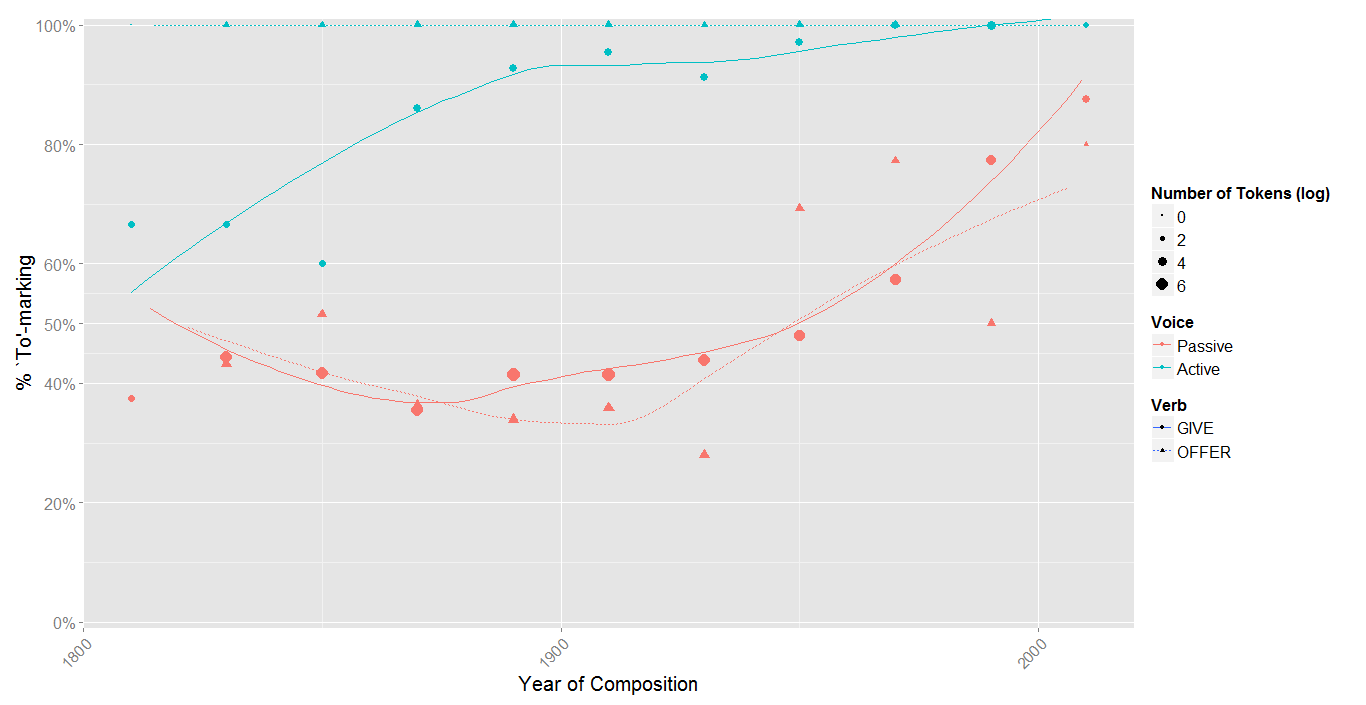
\includegraphics[width=\linewidth]{recpro_to_am}}\\
\label{Fig:topros}
\caption{Data binned in 20 year chunks and loess fits for `to'-marking data from sentences with pronominal recipients. (a) figures compare British and binned American data, while (b) figures compare GIVE and OFFER in American English.}
\end{figure}


When the recipient is a pronoun, bare recipients are much more frequent in British English. There is no significant interaction between year and voice (p=.16), nor a main effect of year (.36) or voice (p=.74). Just as with full noun phrases, recipient pronouns seem to be fairly stable in British English. In this case, the lack of significance may be due to a lack of power, since there are only 155 active tokens and 125 passive tokens across the entire 500 year period.

In American English, active and passive contexts quickly and clearly diverge. In order to better examine the active cases, all active GIVE tokens with `it' after the verb were hand coded. Even with this exhaustive dataset, bare recipients in theme--recipient actives were gone by 1940. After 1940, there are 22 examples of bare theme--recipient actives (out of 3098 tokens of theme--recipient actives with \textit{it} as the theme), all of which occur either in intentionally archaising contexts (e.g. translations of Norse sagas) or in direct quotations in plays or fiction. The restriction to archaising and quotational environments suggest that there was still an awareness of this use of bare recipients in active theme--recipient contexts, but that it was no longer a productive part of the grammar of Standard American English. This can also be seen by the fact that OFFER has no examples of active bare recipients.

In the passive, however, bare recipient pronouns remained common until about 1930, when they start going away. Up until 1930 there is no significant interaction between verb and year (p=.26), nor a main effect of verb (p=.56) or year (p=.67). However, after 1930, there is a significant effect of year (p\textless .01), with no significant interaction with verb (p=.94) or main effect of verb (p=.65). This means that it is only during the 20th century that bare pronominal recipients in theme passives were lost. Indeed, they still occur in 21st century American texts, as can be seen in the following examples: 

\begin{exe}
\ex 
\begin{xlist}
\ex he would fall a long, long way before it would be given him to understand whether any new life was left in him. (COHA, Southern Reverend)
\ex  ... accepting whatever work was given me (COHA, Science Fiction and Fantasy Magazine)
\ex ... and a frayed quilt, which had been given her when she was born. (COHA, Wrong Man)
\ex ... even if it were offered me. (COHA, Thomas, the Rhymer : A romance)
\end{xlist}
\end{exe}

As far as can be seen from the Parsed Corpora of Historical English, written British English has shown complete stability with respect to the use of bare recipients (after 1400). In American English, bare recipients in active contexts was always extremely rare with full noun phrase recipients, and was lost for pronominal recipients by 1940. With theme passives, bare recipients only began to be lost around 1930/1940. During the 19th and early 20th century the use of bare recipients either increased (with full noun phrase recipients) or stayed constant (with bare pronominal recipients).

\section{Conclusion}
As discussed above, a scrambling analysis of the theme--recipient order predicts that the status of the theme should be more relevant for determining word order (since it is the element being targeted for movement). The word order changes in American English are consistent with this idea. While American English appears to still be in the middle of change, for the past 200 years, it has been developing into a system where ditransitive word order is determined primarily by the status of the theme (full noun phrase vs. pronominal). If the change went to completion, pronominal themes would continue to obligatorily precede recipients, and full noun phrase themes would obligatorily follow them. 

With respect to `to' marking, our analysis predicted the observed dissociation of active and passive bare recipients. Bare recipient in active constructions were already marginal in early American English, and were completely eliminated by the early 20th century. Bare theme passives, however, persist throughout the 20th century (and still occur in 21st century American texts). These facts strongly argue against analyses of bare theme passives that rely on deriving them from bare active constructions (see for example \citet{Haddican.2010,Haddican.2011,Haddican.2012}).

Indeed, bare theme passives became more prevalent during the 19th century. We suggest that this may be derived from a surface interpretation of the locality constraint discussed in our analysis. Namely, since the only element intervening between the recipient and the verb is never phonologically realised (the trace), language learners began to more frequently move the theme directly to subject position. We further suggest that bare theme passives were replaced primarily by recipient passives rather than `to'-marked theme passives. Raising the theme across the recipient in the passive is a marked construction cross-linguistically (in so far as it is a surface violation of locality) and thus presumably requires sufficient evidence in the Primary Linguistic Data to be acquired. As recipient passivisation became more common, opportunities for bare theme passives (the only evidence of raising the theme across the recipient) become rarer. Eventually, language learners fail to receive enough evidence to learn the marked construction and bare theme passivisation is lost.

In conclusion, the main change in American English is in the distribution of word orders, with recipient--theme orders becoming more prevalent in cases with full noun phrase themes. The difference in `to' marking between British and American English is dissociated for active and passive cases. Bare recipients with theme pronouns in active clauses was already rare at the start of the American English period, and is lost by the early 20th century. Bare theme passives are only lost in the late 20th century, when they are replaced primarily with recipient passives as part of the aforementioned shift towards recipient--theme word orders.


\part{Introduction}
\chapter{Introduction}

The goal of this work is to provide a summary of the possible grammars in the Northwest Germanic languages (not Gothic) vis-a-vis recipient arguments. There are three major points of variation amongst the languages: (1) type and distribution of recipient marking, (2) linearisation of the recipient with the theme in active sentences, and (3) passivisation. The goal is to provide both a syncronic discription of the range of possible grammars, of both the modern standard Germanic languages (as well as some relevant dialect variation) as well as relevant distinct historical stages. When earlier stages of the languages differ from the modern forms, I will show what different pathways of change have occured. 

Previous work has compared different sub-groups of the modern Germanic languages and between Germanic languages and languages from other families \citep[and others]{Falk.1990, Holmberg.1995, Sprouse.1995, Weerman.1997, Holmberg.1998, Primus.1998, Anagnostopoulou.2003, McFadden.2004, Platzack.2005, Bardal.2006, Heine.2010, Alexiadou.2013, Johannessen.2013, Haddican.2014}; studied the history of a particular Germanic language or language sub-family \citep[and others]{Burridge.1993, Kristoffersen.1994, Kiparsky.1997, Allen.1999, Bardal.2001b, McFadden.2002, Hoskuldurrainsson.2004, Sigursson.2012}; studied the ditransitive construction within a particular language or comparison between dialects (see citations in the individual language sections below). 

This work, as far as I know, is the first to bring all of these pieces of research together, in order to see what generalisations hold over the language family as a whole. By focusing on a particular language family, it is possible to rely on their large set of common features to see how small changes in one area of the grammar effect change in another aspect. This seems to me to be the closest that we can come to the experimental paradigm within historical-comparative linguistics. In order to facilitate comparison, and to avoid prejudicing the study one way or the other, I have focused on a semantic object as the domain of interest, namely recipients. This is under the assumption that while the syntactic and morphological realisation of this role may vary from language to language, the concept is one that all of the languages studied need to have some means to express.  This also gives a construction and morphology independent way to refer to the different arguments that will be used throughout the text: \textbf{agent}, \textbf{recipient} and \textbf{theme}.

For my purposes, I will be focusing on recipients narrowly defined, i.e. recipient arguments of verbs for which the argument is unambiguously a recipient, i.e. the new possessor at the end of a transfer action excluding verbs of motion. This means that out of the list of seven types of recipient introducing verbs discussed in \cite{Hovav.2008}, only (\ref{give}) and (\ref{promise}) will be focused on here. These verbs have an agent, who was the previous possessor of the theme, the theme, which is the object to be transferred, and the recipient, who is the new possessor after the event (e.g. ``The agent gave the recipient the theme''). However, with less studied languages/dialects, where the only data about recipients occurs with some other verbs, data from other categories will be included. 

\begin{exe}
\ex
\begin{xlist}
\ex\label{give} Verbs that inherently signify acts of giving: give, hand, lend, loan, pass, rent sell, ...
\ex \label{promise} Verbs of future having: allocate, allow bequeath, grant, offer, owe, promise, ...
\ex \label{tell} Verbs of communication: tell, show, ask, teach, read, write, quote, cite, ...
\ex \label{send} Verbs of sending (\emph{send}-type verbs): forward, mail, send, ship, ...
\ex \label{throw} Verbs of instantaneous causation of ballistic motion (\emph{throw}-type verbs): fling, flip, kick, lob, slap, shoot, throw, toss, ...
\ex \label{bring} Verbs of causation of accompanied motion in a deictically specified direction: bring, take
\ex \label{fax} Verbs of instrument of communication: e-mail, fax, radio, wire, telegraph, telephone, ...
\end{xlist}
\end{exe}

I give a summary of the types of parameters that I have found to vary among the Germanic languages, starting with types of recipient marking (\autoref{sec:marking}), followed by active word order (\autoref{sec:actwo}), and finally a discussion of passivisation (\autoref{sec:paswo}). This is followed by an introduction to Northwest Germanic languages,  and an in-depth discussion of the data from each language. When there has been a major change in the use of recipients in the recorded history of the language, each distinct historical stage gets its own treatment. Dialect variation on the other hand is treated along side the description of the standard languages (\autoref{part:langg}). The goal is for each language section to stand independently, so that someone interested in a particular language can find all the relevant information in that language's section. This will necessitate repeating information for closely related languages. In \autoref{Conc}, I conclude by drawing together generalisation about the range of possible grammars (\autoref{chap:synchgen}), followed by a discussion of diachronic connections between the different grammar types (\autoref{chap:diagen}). Next, I discuss the theoretical implications of these generalisations. Finally, I collate the remaining questions, whose answers are needed to fill in holes in various language/dialect parameter settings and open theoretical questions (\autoref{chap:furtherquest}). 

\chapter{Parameters}

\section{Recipient Marking}\label{sec:marking}
All of the Germanic languages have at least a subjective (nominative) vs. objective (accusative and dative) system among pronouns. Among some of the languages, there is a distinct dative case that recipients can be marked with. Other of the languages have a prepositional marking system (e.g. English ``to''), which can be used to differentiate between the two objects. Most of the languages, thus, have three different possible markings that a recipient can take in any construction: subjective marking (e.g. nominative case), objective marking (e.g. accusative case), and recipient marking (e.g. dative case or prepositional marking). For each language, I lay out a brief description of the case system for that language, and whether or not it has prepositional marking. In the next two sections, I provide a number of different configurations (which consist of combinations of particular properties, such as the pronominal vs nominal status of the arguments). For each of these configurations, it is possible for recipient marking to vary, which will be discussed in the data sections for each particular language.

\section{Active Word Order}\label{sec:actwo}
The main parameter here is the relative order of the theme and recipient. The standard word order for all the Germanic languages is recipient--theme (e.g. ``I gave John the book.'') The parameter is whether or not the language allows the theme--recipient word order (e.g. ``I gave the book to John.'') This parameter intersects with two other properties: (1) the nominal vs. pronominal status of the recipient and theme and (2) whether or not scrambling or object shift has taken place (i.e. whether or not the objects are still within the verb phrase). This leads to 16 possible post-subject configurations (\ref{tab:activeorders}, in which this parameter could potentially vary.

\begin{table}[h!]
\begin{tabular}{ccccccc}
&&& \multicolumn{4}{c}{Recipient}\\
&&& \multicolumn{2}{c}{Noun} & \multicolumn{2}{c}{Pronoun}\\
&&& Scrambled & Not Scrambled & Scrambled & Not Scrambled\\
{\multirow{4}{*}{Theme}}&{\multirow{2}{*}{Noun}}&Scrambled&RT or TR&RT or TR&RT or TR&RT or TR\\
&&Not Scrambled&RT or TR&RT or TR&RT or TR&RT or TR\\
&{\multirow{2}{*}{Pronoun}}&Scrambled&RT or TR&RT or TR&RT or TR&RT or TR\\
&&Not Scrambled&RT or TR&RT or TR&RT or TR&RT or TR\\
\end{tabular}
\caption{Possible active configurations (RT = `Recipient--Theme, TR = `Theme--Recipient'}
\label{tab:activeorders}
\end{table}

 I am ignoring pre-subject configurations (e.g. topicalisation, ``Books, I gave John'' and wh-movement ``Who did I give the books to?''), as well as rightward dislocation, which is an A' process that moves objects to the right of VP material (e.g. heavy NP shift ``I gave the books yesterday to the man that I met last summer''), because all of these constructions involve further movement of the objects whose pre-movement order is difficult to reconstruct.

\section{Passivisation and Recipient Subjects}\label{sec:paswo}
For the purposes of this work, I will be adopting an inclusive definition of passivisation, namely: a passive sentence is a sentence with a marked form of the verb, in which the agent is optional, but it still implicit if not expressed. With passivisation, the major parameter is usually given as which object raises to subject position, which \cite{Allen.1999} gave the titles of theme and recipient passives. I suggest that there are two other possible passivisation configurations. The first is an expletive passive, where neither argument raises to subject position, but instead an expletive pronoun fills the subject position. Finally, \cite{McCloskey.1997} describes how one of the major innovations of the generative program was to remove subjecthood as a primative notion, instead associating the properties of subjecthood with a structural position. After the late 80s, and the development of the VP-internal subject hypothesis, properties of subjecthood were split, some being derived from the subjects base position within the lower part of the clause, and some being derived by movement to the higher subject position. For the purposes of dealing with passivisation, only this higher position is relevant, since the objects are presumably base generated in their object positions. Note that there is no principled reason within such a framework for assuming that all sentences have subjects, or that all languages have the higher subject position. In such a language, there is no notion of subject, which would thus create a subjectless passive. For any language (or historical stage of a language), there needs to be some evidence that subjects exist; only then can it be sensibly asked which argument can become the subject in the passive. This means that there are four possible settings for this parameter. In languages without subjects, only the subjectless passive is possible. In the other languages, a particular configuration can either allow recipient, theme, expletive passive, or some combination of them all.

When discussing the individual languages, I will describe what properties are being associated with a subject position. Note that this generative notion of subject requires that these properties be correlated with a particular position for subjects. In V2 clauses, this position is either immediately before or after the finite verb depending on whether there is another element in the preverbal position. Two major properties that have been associated with subjects that are certainly not subject properties according to this restricted definition: nominative case and verb agreement. \cite{Bardal.2000} makes this methodological point, namely that after the discovery of oblique subjects and nominative objects in Icelandic (see \autoref{sec:Icelandic} below for details), it was no longer possible to assume that neither nominative case nor the associated verbal agreement can be viewed as properties of subjects alone. Thus, while case marking patterns with recipients and themes in ditransitive passives will be discussed, they will not be viewed as giving evidence to the subject vs. non-subject status of arguments.

As with the active orders, the nominal vs. pronominal status of both the theme and recipient are relevant for this parameter as well. Also relevant for some of the languages the type of passive verbal marking is relelvant, either by having different passive auxilaries (be/become vs. get), or by having synthetic passive marking instead of a passive auxiliary (Scandinavian -s- passive). Even in subjectless languages, the arguments can receive different case/prepositional marking in the different configurations, which will be addressed in the data for the individual languages. Combining all the possible variables means that there are a maximum of twelve different configurations as seen in \autoref{tab:pasorders}. 

\begin{table}[h!]
\begin{tabular}{ccccc}
& \multicolumn{2}{c}{Recipient Noun} & \multicolumn{2}{c}{Recipient Pronoun}\\
& Theme Noun & Theme Pronoun & Theme Noun & Theme Pronoun\\
Be/become auxiliary & RP, TP, EP or SP & RP, TP, EP or SP & RP, TP, EP or SP & RP, TP, EP or SP\\
Get auxiliary & RP, TP, EP or SP & RP, TP, EP or SP & RP, TP, EP or SP & RP, TP, EP or SP\\
-s- passive & RP, TP, EP or SP & RP, TP, EP or SP & RP, TP, EP or SP & RP, TP, EP or SP\\
\end{tabular}
\caption{Possible passive configurations (RP = `Recipient Passive, TP = `Theme Passive', EP = `Expletive Passive`, SP = `Subjectless Passive }
\label{tab:activeorders}
\end{table}

With respect to `get', \cite{Broekhuis.1994} argues that in at least some of the Germanic languages, `get' can act as a passive auxiliary. When that happens, `get' co-occurs with a passive participle, which heads the verb phrase and introduces the nominal arguments. This is different from what they call the ``undative'' meaning of `get'. `Get' as a verb introduces a recipient as its subject and a theme as its object. \cite{Broekhuis.1994} suggest that in both the `undative' and passive uses of `get', the recipient subject starts out low and raises to subject position. My focus in this work is on the use of `get' as a passive auxiliary, and how the construction it introduces differs from the other passive constructions.

\part{Language Data}\label{part:langg}
\chapter{Introduction to Northwest Germanic}
Northwest Germanic consists of the modern Germanic languages and their ancestors, to the exclusion of East Germanic (of which Gothic is the only daughter language for which any substantial evidence remains). The major divide in the family is between North Germanic (Scandinavian) and West Germanic. Among the North Germanic languages, historically there was a split between Norse in the west, which was the ancestor of Icelandic, Faroese and Norwegian, and East Scandinavian, which was the ancestor of Danish and Swedish. By the Middle Ages, however, the division between the Insular Scandinavian languages on the one hand (Icelandic and Faroese) and the Mainland Scandinavian languages on the other (Norwegian, Swedish and Danish) became much more relevant. Among the West Germanic group, the first major historical division is between the West Germanic group proper (the ancestor of Dutch, Afrikaans, High German and Yiddish), and the Ingvaeonic languages (the ancestors of Frisian, Low German, and Old English). Again, more recently the difference between Insular West Germanic (i.e. English) and the mainland languages has become more pronounced. Also Dutch (and its daughter Afrikaans) have begun to pattern more with the continental Ingvaeonic languages (i.e. Frisian and Low German). Both Frisian and Low German, on the other hand, have undergone strong sociolinguistic pressure from both Dutch, High German (and to a smaller extent Danish).

For each of the language family below, the structure of the description is the same. I start with older forms of the languages, and then move towards the modern period, when significantly different stages can be identified. Within each stage of the language, I start with an introduction to that stage, describing its location in both time and space, and describing the extant data, either in the form of written corpora, or current speakers. I then discuss the case marking system of the language, as well as the possibility of using prepositional marking with recipients. Then I go through the possible Active configurations and discuss what word order and case/prepositional marking patterns are permitted in that configuration, or demonstrate that the configuration itself is unattested/ungrammatical. Finally, I discuss the passive, starting with a discussion of subject properties (or lack thereof) in the language, and followed by a description of the parameter settings for all of the possible passive configurations (which will include both `'be/become'' and `'get'' passives in all the languages, but -s- passives only in Scandinavian).
\chapter{Scandinavian}
\section{Old Scandinavian}\label{sec:OldScand}

\subsection{Introduction}
Old Scandinavian is the set of dialects spoken in the Scandinavian nations before 1500. There are four distinct dialects, although they are often described as being fairly homogenous with respect to syntax. The most studied dialect is Old Norse, which consists of documents written in Iceland. Closely related to Old Norse is Old Norwegian. More divergent are the Eastern languages Old Swedish and Old Danish.
\subsection{Case and Preposition Marking}
Most of the Old Scandinavian dialects still maintained the distinction between nominative, accusative and dative case in both full noun phrases and pronouns. On the other hand, most Old Danish dialects had already lost synthetic case marking in noun phrases by the earliest texts (circa 1350). CHECK ON OLD DANISH PRONOUN CASE SYSTEM. There is no evidence that any of the Old Scandinavian languages had prepositional marking of recipients.

\subsection{Active Word Orders}
In the active, both word orders are found, although in Old Norse (as represented by ICEPAHC), there is a change in word order throughout the Old Norse period, where the theme-recipient word order becomes less available. The only configuration in which the recipient-theme word order does not become more common is when the recipient is a noun and the theme is a pronoun, where the recipient-theme order occurs on average  50\% of the time throughout the Old Scandinavian period. For the remaining configurations, during the last century of the Old Scandinavian period, the recipient-theme order occurs 92.8571\% of the time.

\begin{knitrout}
\definecolor{shadecolor}{rgb}{0.969, 0.969, 0.969}\color{fgcolor}\begin{figure}[p!]


{\centering \includegraphics[width=\linewidth]{figure/lang-oiact-graph} 

}

\caption[LOESS lines for Old Scandinavian active sentence from IcePaHC]{LOESS lines for Old Scandinavian active sentence from IcePaHC.\label{fig:oldscanactgraph}\label{fig:oiact-graph}}
\end{figure}


\end{knitrout}

\subsection{Passive}
\subsubsection{Subjecthood}
\cite{Bardal.1997,Bardal.1998,Bardal.2000,Bardal.2001} argues that Old Scandinavian shows the same constructions as Modern Icelandic, and therefore should be considered to have oblique subjects (Her focus is on experiencer verbs, insead of recipient verbs). \cite{Rognvaldsson.1991}, again about dative experiencers, states: ``I have not found a signle case where inverted oblique subject-like NPs follow the main verb, they always immediately follow the finite verb.'' This seems to indicate that in Old Scandinavian, as in Modern Icelandic, the standard V2 subject position exists (i.e. immediately before the finite verb, if there is no fronted element, and immediately after the finite verb if some element has been fronted). However, I have found at least one example in IcePaHC where there is nothing in the subject position. The following (passive) example has a fronted temporal adverb, and then nothing in between the finite verb and the main verb (i.e. in the subject position). Both of the objects are presumably still in-situ in the verb phrase.
\begin{exe}
\ex \gll Nú er sagt konungi dráp ármannsins\\
now was said king.DAT killing.NOM/ACC Herman.GEN.his.GEN\\
\trans `Now the king was told of the killing of Herman. (IcePaHC, 1275.MORKIN.NAR-HIS,.667)'
\end{exe}
Far more examples, however, have a nominal element which does occur in one of the subject positions. 
\begin{exe}
\ex
\begin{xlist}
\ex \gll Málróf er gefið mörgum\\
Málróf is given much\\
\trans `Málróf is given much.'
\ex \gll en annan dag jóla var hann í jörð lagður\\
and the day Christmas was he in earth laid\\
\trans `and on the day after Christmas he was laid in the earth. (IcePaHC, 1210.THORLAKUR.REL-SAG,.489)'  
\end{xlist}
\end{exe}
 \cite{Kinn.2010} suggests, discussing Old Norwegian, that in the early period, the subject position existed, but was not obligatorily filled. This seems to correspond to the situation in IcePaHC, where most clauses have subjects, but some small number do not.
\subsubsection{Be/Become Passive}
There are not enough passive tokens in IcePaHC to see any historical trajectory. However, when collating the data from the entire Old Icelandic period, it can be seen that recipient passivisation seems to have been the preferred strategy across the board. This is especially true when the recipient is a pronoun, but there seems to be strong tendencies towards recipient passivisation even with full noun phrase recipients. The theme empty category includes both wh-moved elements and pro-dropped elements, either under pragmatic conditions or under conjunction.

% latex table generated in R 3.1.0 by xtable 1.7-3 package
% Mon Sep 01 13:03:19 2014
\begin{table}[ht]
\centering
\begin{tabular}{rlll}
  \hline
 & Theme Empty & Theme Noun & Theme Pronoun \\ 
  \hline
Recipient Noun & 0\% (3) & 76.2\% (21) & 66.7\% (3) \\ 
  Recipient Pronoun & 100\% (13) & 90.5\% (21) & 100\% (4) \\ 
   \hline
\end{tabular}
\caption{Passive Recipient Passivisation Rates in Old Icelandic (Total Token Numbers in Parentheses)} 
\end{table}



\subsubsection{Get Passive}
I have no information about `get'-passives in Old Scandinavian, however, based on Modern Icelandic, it is likely that the languaged lacked `get' as a passive auxiliary.
\subsubsection{-s- Passive}
The -s- morpheme, which is historically a reduced form of the anaphoric pronoun (e.g. German \emph{sich} `himself') had a middle function in Old Icelandic.

\section{Modern Icelandic}\label{sec:Icelandic}
\subsection{Introduction}
Spoken in Iceland from 1500.
\subsection{Case and Preposition Marking}
Icelandic has distinct nominative, dative and accusative cases for both nouns and pronouns:
\begin{exe}
\ex Noun phrases:
 \gll Pétur gaf konunginum ambáttina.\\
Peter.NOM gave king.DEF.DAT maid-servant.DEF.ACC\\
\trans `Peter gave the king the maid-servant.'
\ex Pronouns:
\gll Hann sýndi henní hana oft\\
he.NOM showed her.DAT it.ACC often\\
\trans `He often showed her it.'
\end{exe}
Preposition marking with \emph{til} `to' is restricted to a small set of recipients, for which animacy seems to be relevant. (\ref{ex:icetil}).
\begin{exe}
\ex \label{ex:icetil} \cite{Ottosson.1993} 
\begin{xlist} 
\ex[*] {\gll Jón gaf bókina til Maríu\\
John gave book.DEF to Mary\\
\trans `John gave the book to Mary.'}
\ex \gll Jón gaf bókasafn sitt til háskólans\\
John gave library {his own} to university.DEF\\
\trans `John donated his own library to the university.'
\end{xlist}
\end{exe}
\subsection{Active Word Order}
\subsubsection{Both Nouns}
Looking at cases where both the recipient and the theme are full noun phrases, there is some disagreement about the possible word orders. Some scholars have reported that both word orders are allowed, in cases where both the theme and recipient are animate (\ref{ice:bothanimateact}). \cite{Dehe.2004} found that her naive Icelandic informants reported the theme-recipient word order degraded/ungrammatical with almost all variations (including IO focus and shared animacy). 
\begin{exe}
\ex\label{ice:bothanimateact}
\begin{xlist}
\ex \gll Hann gaf konunginum ambáttina.\\
He.NOM gave king.DEF.DAT maid-servant.DEF.ACC\\
\trans `He gave the king the maid-servant. \citep[ex 14a]{Dehe.2004}
\ex[?*] {\gll Hann gaf ambáttinakonunginum.\\
He.NOM gave maid-servant.DEF.ACC king.DEF.DAT \\
\trans `He gave the king the maid-servant. \citep[ex 14b]{Dehe.2004}}
\end{xlist}
\end{exe}
For some speakers the theme-recipient order was improved by making the recipient heavy:
\begin{exe}
\ex
\begin{xlist}
\ex \gll Stefán gaf Hildi sem býr á Akureyri sítrónuna. \\
Stefan gave H.DAT Rel-part(who) is from Akureyri lemon.DEF.ACC\\
\trans `Stefan gave Hildi who is from Akureyri the lemon. \citep[ex 16b]{Dehe.2004}'
\ex[?] {\gll Stefán gaf sítrónuna Hildi sem býr á Akureyri \\
Stefan gave lemon.DEF.ACC H.-DAT Rel-part(who) is from Akureyri \\
\trans `Stefan gave the lemon to Hildi who is from Akureyri. \citep[ex 16a]{Dehe.2004}'}
\end{xlist}
\end{exe}
When it comes to object shift, an operation that moves some objects to the left of VP level adverbs as well as negation, either object can move, but only the recipient--theme word order is permitted.
\begin{exe}
\ex \cite[ex. 47]{Vikner.1989}
\begin{xlist}
\ex \gll Pétur sýndi oft Mariú bokína\\
Pétur showed often Mary.DAT book.DEF.ACC\\
\trans `Pétur often showed Mary the book.'
\ex[]{\gll Pétur sýndi Mariú oft bokína\\
Pétur showed Mary.DAT often book.DEF.ACC\\
\trans `Pétur often showed Mary the book.'}
\ex[]{\gll Pétur sýndi Mariú bokína oft\\
Pétur showed Mary.DAT book.DEF.ACC often\\
\trans `Pétur often showed Mary the book.'}
\ex[*]{\gll Pétur sýndi oft bokína Mariú\\
Pétur showed often book.DEF.ACC Mary.DAT\\
\trans `Pétur often showed the book to Mary.'}
\ex[*]{\gll Pétur sýndi bokína oft Mariú\\
Pétur showed book.DEF.ACC often Mary.DAT\\
\trans `Pétur often showed the book to Mary.'}
\ex[*]{\gll Pétur sýndi bokína Mariú oft\\
Pétur showed book.DEF.ACC Mary.DAT often\\
\trans `Pétur often showed the book to Mary.'}
\end{xlist}
\end{exe}
\subsubsection{Recipient Pronoun}
When the recipient is a pronoun, but the theme is a noun, the same general word order trend remains, except that it is odd for the pronoun not to undergo object shift. The theme still cannot precede the recipient.
\begin{exe}
\ex \cite[ex. 48]{Vikner.1989}
\begin{xlist}
\ex[??]{\gll Pétur sýndi oft henní bokína\\
Pétur showed often her.DAT book.DEF.ACC\\
\trans `Pétur often showed her the book.'}
\ex[]{\gll Pétur sýndi henní oft bokína\\
Pétur showed her.DAT often book.DEF.ACC\\
\trans `Pétur often showed her the book.'}
\ex[]{\gll Pétur sýndi henní bokína oft\\
Pétur showed her.DAT book.DEF.ACC often\\
\trans `Pétur often showed her the book.'}
\ex[*]{\gll Pétur sýndi oft bokína henní\\
Pétur showed often book.DEF.ACC her.DAT\\
\trans `Pétur often showed the book to her.'}
\ex[*]{\gll Pétur sýndi bokína oft henní\\
Pétur showed book.DEF.ACC often her.DAT\\
\trans `Pétur often showed the book to her.'}
\ex[*]{\gll Pétur sýndi bokína henní oft\\
Pétur showed book.DEF.ACC her.DAT often\\
\trans `Pétur often showed the book to her.'}
\end{xlist}
\end{exe}
\subsubsection{Theme Pronoun}
When the theme is a pronoun, and the recipient is a noun phrase, only one word order is possible, namely both objects must undergo object shift. The theme needs to undergo object shift since it is a pronoun, and since the theme cannot precede the recipient, the recipient must also undergo object shift so that it will still precede the theme.
\begin{exe}
\ex \cite{Vikner.1989}
\begin{xlist}
\ex[*]{\gll Pétur sýndi oft Mariú hana\\
Pétur showed often Mary.DAT it.ACC\\
\trans `Pétur often showed Mary it.'}
\ex[*]{\gll Pétur sýndi Mariú oft hana\\
Pétur showed Mary.DAT often it.ACC\\
\trans `Pétur often showed Mary it.'}
\ex[]{\gll Pétur sýndi Mariú hana oft\\
Pétur showed Mary.DAT it.ACC often\\
\trans `Pétur often showed Mary it.'}
\ex[*]{\gll Pétur sýndi oft hana Mariú\\
Pétur showed often it.ACC Mary.DAT\\
\trans `Pétur often showed it to Mary.'}
\ex[*]{\gll Pétur sýndi hana oft Mariú\\
Pétur showed it.ACC often Mary.DAT\\
\trans `Pétur often showed it to Mary.'}
\ex[*]{\gll Pétur sýndi hana Mariú oft\\
Pétur showed it.ACC Mary.DAT often\\
\trans `Pétur often showed it to Mary.'}
\end{xlist}
\end{exe}
\subsubsection{Both Pronouns}
When both objects are pronouns, the same restrictions applied as when only the theme was a pronoun, since the theme wants to object shift, and the recipient must object shift as well. In this case, the recipient independently would need to undergo object shift, since it is itself a pronoun.
\begin{exe}
\ex \cite[ex 50]{Vikner.1989}
\begin{xlist}
\ex[*]{\gll Pétur sýndi oft henní hana\\
Pétur showed often her.DAT it.ACC\\
\trans `Pétur often showed her it.'}
\ex[*]{\gll Pétur sýndi henní oft hana\\
Pétur showed her.DAT often it.ACC\\
\trans `Pétur often showed her it.'}
\ex[]{\gll Pétur sýndi henní hana oft\\
Pétur showed her.DAT it.ACC often\\
\trans `Pétur often showed her it.'}
\ex[*]{\gll Pétur sýndi oft hana henní\\
Pétur showed often it.ACC her.DAT\\
\trans `Pétur often showed it to her.'}
\ex[*]{\gll Pétur sýndi hana oft henní\\
Pétur showed it.ACC often her.DAT\\
\trans `Pétur often showed it to her.'}
\ex[*]{\gll Pétur sýndi hana henní oft\\
Pétur showed it.ACC her.DAT often\\
\trans `Pétur often showed it to her.'}
\end{xlist}
\end{exe}
\subsubsection{Summary}
The above examples show that the recipient is always marked with dative case in the active. With respect to the word order parameter, already in Early Modern Icelandic (c. 1500) the recipient-theme word order was predominant (at a rate of $\sim$90.678\%) in almost all conditions. The final environment, where the theme-recipient word order remained a viable possibility was where the recipient was a full noun phrase and the theme a pronoun. Starting around 1800 this condition began to change, such that by the present day it joined all the other conditions in requiring the recipient-theme word order (see \ref{fig:modscanactgraph}).

\begin{knitrout}
\definecolor{shadecolor}{rgb}{0.969, 0.969, 0.969}\color{fgcolor}\begin{figure}[p!]


{\centering \includegraphics[width=\linewidth]{figure/lang-miact-graph} 

}

\caption[LOESS lines for Modern Icelandic active sentence from IcePaHC]{LOESS lines for Modern Icelandic active sentence from IcePaHC.\label{fig:modscanactgraph}\label{fig:miact-graph}}
\end{figure}


\end{knitrout}

\subsection{Passive}
\subsubsection{Subjecthood}
\cite{Zaenen.1985} gives the classic presentation of the evidence in Modern Icelandic for oblique subjects. I can be seen below that there are two positions that are subject positions, which both the recipient and theme can fill in the passive. The first is directly after the raising predicate (e.g. `believe'). The second is the post-finite verb position. Both of these positions can be filled only by the subject in clauses with uncontested subjects.
\begin{exe}
\ex 
\begin{xlist}
\ex Raising
\begin{xlist}
\ex \gll \'{E}g tel konunginum hafa veri\dh gefnar amb\'{a}ttir.\\
I believe king.the.DAT have been given slaves.NOM.\\
\trans `I beleive the king to have been given slaves \citep{Zaenen.1985}.'
\ex \gll \'{E}g tel amb\'{a}ttir hafa veri\dh gefnar konunginum.\\
I believe slaves.NOM have been given king.the.DAT.\\
\trans `I beleive the king to have been given slaves \citep{Zaenen.1985}.'
\end{xlist}
\ex Subject verb inversion
\begin{xlist}
\ex \gll Um veturinn voru konunginum gefnar amb\'{a}ttir.\\
In winter.the were king.the.DAT given slaves.NOM\\
\trans `In the winter the king was given slaves `\citep{Zaenen.1985}.
\ex \gll Um veturinn voru amb\'{a}ttin gefin konunginum.\\
In winter.the were slave.NOM given king.the.DAT\\
\trans `In the winter slaves were given to the king \citep{Zaenen.1985}.'
\ex \gll Voru konunginum gefnar amb\'{a}ttir?\\
were king.the.DAT given slaves.NOM?\\
\trans `Was the king given slaves?`\citep{Zaenen.1985}.
\ex \gll Var amb\'{a}ttin gefnar konunginum?\\
were slave.NOM given king.the.DAT'?\\
\trans `Was a slave given to the king? \citep{Zaenen.1985}.'
\end{xlist}
\end{xlist}
\end{exe}
\subsubsection{Be/Become Passive}
As discussed previously, both theme and recipient passivisation are possible in Modern Icelandic, in passive clauses with `be' or `become' as passive auxiliaries. In both constuctions, the theme is in nominative case and the recipient in dative case. 

\begin{exe}
\ex 
\begin{xlist}
\ex \gll J\'{o}ni var gefin b\'{o}kin.\\
John.DAT was given book.the.NOM\\
\trans `John was given the book \citep{Holmberg.1995,Bardal.2001}.'
\ex \gll B\'{o}kin var gefin J\'{o}ni.\\
book.the.NOM was given John.DAT\\
\trans `The book was given to John \citep{Holmberg.1995,Bardal.2001}.'
\end{xlist}
The nominative argument always shows agreement with the auxiliary \citep[98]{Arnadottir.2013}.
\end{exe}
\begin{exe}
\ex
\begin{xlist}
\ex[] {\gll {Í gaer} voru bílarnir gefið mér\\
Yesterday were.3PL cars.the.M.PL.NOM given.DEF me.DAT\\
\trans `Yesterday, the cars were given to me.' }
\ex[*] {\gll {Í gaer} var mér gefið bílarnir\\
Yesterday was.3SG me.DAT given.DEF cars.the.M.PL.NOM\\
\trans `Yesterday, I was given the cars.'}
\end{xlist}
\end{exe}
Traditionally, expletive passives are not grammatical, although this has changed in recent years.This so-called ``New Passive'', in which both argument remain in their active word order position with the active case marking, has started to be accepted by the youngest generation of speakers. 
\begin{exe}
\ex[\%] {\gll {Í gaer} var mér gefið bílana \\
yesterday was.3SG me.DAT given.DEF cars.the.M.PL.ACC \\
\trans `Yesterday I was given the cars.' }
\end{exe}
Finally, there are a small number of speakers who are accepting two new case marking patterns in the recipient passive. A fairly substantial number of speakers are marking the theme with the accusative case in the recipient passive.
\begin{exe}
\ex[\%] {\gll mér var gefið bílana \\
me.DAT was.3SG given.DEF cars.the.M.PL.ACC \\
\trans `I was given the cars.' }
\end{exe}
 A much smaller number of speakers are marking the recipient with nominative case in the recipient passive.
 \begin{exe}
\ex[\%] {\gll Ég var gefið bílana \\
I.NOM was.3SG given.DEF cars.the.M.PL.ACC \\
\trans `I was given the cars.' }
\end{exe}
While IcePaHC does not have enough tokens to look at the development of the passive in Modern Icelandic, it does provide some information about average rates throughout the Modern Icelandic period. In most conditions, the recipient passive is the predominant form. While the number of tokens is small, the condition with a theme pronoun and a recipient full noun phrase seems to prefer the theme passive. This is consonant with the pattern of change in the active, where in the Early Modern Icelandic period, this condition was the main holdout for the theme-recipient. The theme empty category includes both wh-moved elements and pro-dropped elements, either under pragmatic conditions or under conjunction.

% latex table generated in R 3.1.0 by xtable 1.7-3 package
% Mon Sep 01 13:03:21 2014
\begin{table}[ht]
\centering
\begin{tabular}{rlll}
  \hline
 & Theme Empty & Theme Noun & Theme Pronoun \\ 
  \hline
Recipient Noun & 85.7\% (7) & 81.2\% (16) & 16.7\% (6) \\ 
  Recipient Pronoun & 85\% (20) & 96.4\% (28) & 66.7\% (9) \\ 
   \hline
\end{tabular}
\caption{Passive Recipient Passivisation Rates in Modern Icelandic (Total Token Numbers in Parentheses)} 
\end{table}

\subsubsection{Get Passive}
\cite{Sigursson.2012b} demonstrates that get constructions in Modern Icelandic do not pattern as passives. Unlike be/become passives only the theme object tends to precede the passive participle, which agrees with the theme object in accusative case. Also, only the recipient is capable of being the subject of `get', no matter what word order or case patterns apply. Instead, it appears that the construction is a typical undative construction, with a recipient subject, and a modified object. This leads to the translation of the `get' construction as `Mary got the sent book.' 
\begin{exe}
\ex
\begin{xlist}
\ex \gll Jón sendi Maríu bókina.\\
Jon.Nom sent Maria.DAT book.DEF.ACC\\
\trans `John sent Mary the book.'
\ex \gll Maríu var send bókin.\\
Mary.DAT was sent.PASS.F.SG.NOM book.DEF.F.NOM\\
\trans `Mary was sent the book.'
\ex \gll María fékk bókina senda.\\
Mary.NOM got book.DEF.F.ACC sent.PASS.F.SG.ACC\\
\trans `Mary got the sent book.'
\end{xlist}
\ex
\begin{xlist}
\ex \gll Nú skal konungur fá ambáttina gefna.\\
now shall king.NOM get maid.servant.the.F.ACC given.PASS.F.SG.ACC\\
‘Now the king will get given the female slave.’
\ex[*] {\gll ∗Nú skal ambáttina fá {konungur} gefna {konungur}.\\
now shall servant.the.F.ACC get king.NOM given.PASS.F.SG.ACC king.NOM\\
\trans INTENDED: ‘Now the servant will get given to the king.’}
\ex[*] {\gll ∗Nú skal amb´attin fá (konungur) gefin (konungur). \\
now shall servant.the.F.NOM get king.NOM given.PASS.F.SG.NOM king.NOM \\
\trans INTENDED: ‘Now the servant will get given to the king.’}
\ex[*] {\gll ∗Nú skal ambáttin fá (konunginum) gefin (konunginum) \\
now shall servant.the.F.NOM get king.the.DAT given.PASS.F.SG.NOM king.the.DAT\\
\trans INTENDED: ‘Now the servant will get given to the king.’}
\ex[*] {\gll ∗Nú skal ambáttina fá (konunginum) gefna (konunginum).\\
now shall servant.the.F.ACC get king.the.DAT given.PASS.F.SG.ACC king.the.DAT\\
\trans INTENDED: ‘Now the servant will get given to the king.’}
\end{xlist}
\end{exe}
\subsubsection{-s- Passive}
The -s- passive in Modern Icelandic, which is historically derived from univerbation of the verb with the reflexive pronoun, shows different patterns with respect to dative object in monotransitive and ditransitive clauses. Monotransitive datives become nominative when in the -s- passive, but the ditransitive datives (including recipients) stay dative in the -s- passive. Unlike the be/become passive, the theme remains marked in accusative instead of becoming nominative. However, unlike the be/become passive, there is no implicit agent in these clauses, and introducing an agent with a `by'-phrase is impossible, which may indicate that in Modern Icelandic this form is still a middle construction as opposed to being a true passive.
\begin{exe}
\ex Monotransitive Verbs
\begin{xlist}
\ex \gll Jón splundraði rúðunni.\\
John shattered window.DEF.DAT\\
\trans `John shattered the window.'
\ex \gll rúðan splundraðist.\\
window.DEF.NOM shattered.PASS\\
\trans `The window shattered.'
\end{xlist}
\ex Ditransitive Verbs
\begin{xlist}
\ex \gll Þeir buðu mér peninga.\\
they.NOM offered me.DAT money.ACC\\
\trans `They offered me money.'
\ex \gll Mér buðust peninga.\\
me.DAT offered.ST money.ACC\\
\trans `I got offered money.'
\end{xlist}
\end{exe}

\section{Faroese}\label{sec:Faroese}



\subsection{Introduction}
\subsection{Case and Preposition Marking}
Faroese has distinct nominative, dative and accusative case forms for both nouns and pronouns. \cite{Lundquist.2013b} notes that prepositional marking with \emph{til} `to' is becoming more common in Faroese.

\subsection{Active Word Order}
When both objects are nouns, either the recipient precedes the theme, or it is marked with the preposition \emph{til}.
\begin{exe}
\ex 
\begin{xlist}
\ex \gll Hon gav Mariu troyggiuna.\\
She gave Maria.DAT sweater.THE.ACC.\\
\trans `She gave Maria the sweater \citep{Lundquist.2013b}.'
\ex[*]{\gll Hon gav troyggiuna Mariu.\\
She gave sweater.THE.ACC Maria.DAT.\\
\trans `She gave the sweater to Maria \citep{Lundquist.2013b}.'}
\ex \gll Hon gav troyggiuna til Mariu.\\
She gave sweater.THE.ACC to Maria.DAT.\\
\trans `She gave the sweater to Maria \citep{Lundquist.2013b}.'
\end{xlist}
\end{exe}
This remains true if both of the objects are pronouns. I do not have data for this, but presumably prepositional marking of the dative could be used here as well to get the reverse word order.
\begin{exe}
\ex \gll Turið gav honum t\ae r\\
Turið gave him.DAT them.ACC\\
\trans `Turið gave him them.'
\end{exe}
Only pronouns are able to undergo object shift in Faroese. Unstressed pronouns obligatorily undergo the shift, although I do not have data on how this interacts with ditransitive cases (e.g. what if the theme is an unstressed pronoun, while the recipient is a full noun phrase).
\subsection{Passive}
\subsubsection{Subjecthood}
Faroese has the typical V2 subject position, i.e. before the finite verb, unless there is another fronted element, in which case it occurs immediately after the finite verb. This position is not tied to case, so subjects can be marked nominative, accusative or dative. This pattern is changing in recent years, with most speakers replacing traditional dative experiencer subjects with nominative experiencers. Only subjects are capable of going between the finite verb and any non-finite complement, which makes it possible to distinguish between oblique subjects and fronted oblique objects.
\begin{exe}
\ex \gll Bóndanum vað kúgvin seld\\
farmer.DEF.DAT was cow.DEF.NOM sold\\
\trans `To the farmer, the cow was sold. \cite[ft. 47]{Hoskuldurrainsson.2004}'
\end{exe}
\subsubsection{Be/Become Passive}
\cite[28]{Barnes.1986} states that: "the usual word-order in passivised sentences with an indirect object is: nominative subject + passive verb + indirect object", i.e. theme passivisation is the preferred strategy.
\begin{exe}
\ex 
\begin{xlist}
\ex \gll Kúgvin varð seld bóndanum\\
cow.DEF.NOM was sold.NOM farmer.DEF.DAT\\
\trans `The cow was sold to the farmer.' \citep[ex. 103]{Barnes.1986}
\ex \gll Ein blýantur varð givin henni\\
a pencil.NOM was given.NOM her.DAT\\
\trans `A pencil was given to her.' \citep[ex. 104]{Barnes.1986}
\end{xlist}
\end{exe}
When the theme is indefinite, recipient passivisation is marginally accepted.
\begin{exe}
\ex
\begin{xlist}
\ex[?] {\gll Bóndanum varð seld kúgvin\\
farmer.DEF.DAT was sold.NOM cow.DEF.NOM\\
\trans `The farmer was sold the cow.' \citep[ex. 98]{Barnes.1986}}
\ex[?] {\gll Henni varð givin ein blýantur\\
her.DAT was given.NOM a pencil.NOM\\
\trans `She was given a pencil.' \citep[ex. 99]{Barnes.1986}}
\end{xlist}
\end{exe}
This can be improved by making the theme relatively heavy and conveying new information, however, theme passivisation is still possible in these configurations.
\begin{exe}
\ex \gll Myndugleikunum vórðu givnar allar upplýsingarnar.\\
authorities.DEF.DAT.PL were given.NOM.PL all.NOM.PL information.DEF.NOM.PL\\
\trans `The authorities were given all the information.'
\ex \gll Allar upplýsingarnar vórðu givnar myndugleikunum.\\
all.NOM.PL information.DEF.NOM.PL were given.NOM.PL authorities.DEF.DAT.PL\\
\trans `The authorities were given all the information.'
\end{exe}
When the theme is given (usually definite), then recipient passivisation is severely degraded or ungramatical.
\begin{exe}
\ex 
\begin{xlist}
\ex[??] {\gll Bóndanum varð selt kúgv\\
farmer.DEF.DAT was sold.NOM cow.DEF.ACC\\
`The farmer was sold the cow.' \citep[ex. 100]{Barnes.1986}}
\ex[??] {\gll Henni varð givið ein blýant\\
her.DAT was given.NOM a pencil.ACC\\
\trans `She was given a pencil.' \citep[ex. 101]{Barnes.1986}}
\end{xlist}
\end{exe}
\cite{Eyorsson.2012} reports results of a grammatical survery of native Faroese speakers, looking into possible case marking patterns with recipient passives. Half of the speakers rejected even the canonical case marking pattern (dative recipient, nominative theme).
\begin{exe}
\ex 25.8\% acceptance vs. 50\% rejection\\
\gll Gentuni bleiv givin ein telda.\\
the.girl.DAT was given.NOM a.Nom computer.NOM\\
\trans `The girl was given a computer. \cite[ex 45a]{Eyorsson.2012}'
\end{exe}
More people rejected a version with an accusative theme and a dative subject. This was with an accusative passive participle. It would be interesting to see how subjects would react to a nominative participle (i.e. showing default agreement).
\begin{exe}
\ex 17.7\% acceptance vs. 61.3\% rejection\\
\gll Gentuni bleiv givið eina teldu.\\
the.girl.DAT was given a.ACC computer.ACC\\
\trans `The girl was given a computer. \cite[ex 45b]{Eyorsson.2012}'
\end{exe}
Even fewer people accepted marking the recipient with nominative case, and having it trigger agreement on both the finite verb and the participle. While this was clearly marginal, more than 1 out of 10 speakers still found this construction grammatical.  This may indicate that the change in case marking that has been seen with Faroese experiencers (dative $\rightarrow$ nominative) is also happening with passive recipient subjects. It would be hard to study this in a corpus, however, due to the overwhelming preference for theme passivisation.
\begin{exe}
\ex 14.5\% acceptance vs. 77.4\% rejection\\
\gll Gentan bleiv givin telduna\\
the.girl.NOM was given.NOM the.computer.ACC\\
\trans `The girl was given a computer. \cite[ex 48b]{Eyorsson.2012}'
\ex[*] {\gll Gentan bleiv givin teldan.\\
the.girl.NOM was given.NOM the.computer.NOM\\
\trans `The girl was given a computer. \cite[ex 48a]{Eyorsson.2012}'}
\end{exe}

\cite[ex 41]{Jonsson.2009b} reports results of a survey of Faroese speakers, with respect to expletive passivisation, which was accepted by more than half of the respondents. 
\begin{exe}
\ex 
\begin{xlist}
\ex \gll Það var sýnt þeim bæklinga áður en þau fóru\\
there was shown them.DAT brochures.ACC before they left\\
\trans `They were shown brochures before they left (52% acceptance vs 12% rejection)'
\ex \gll Var þeim ekki {einu sinni} sýnt íbúðina fyrst?\\
was them.DAT not even shown apartment.DEF.ACC first\\
\trans `Were they not even shown the apartment first? (59% acceptance vs 19% rejection)'
\end{xlist}
\end{exe}

\subsubsection{Get Passive}
I do not have any data on the get passive in Faroese.

\subsubsection{-s- Passive}
In Faroese, the -st- form, which is historically derived from the univerbation of the finite verb with the reflexive pronoun, still retains its reflexive meaning. Even in cases where it seems to have a passive function (i.e. no agent and promotion of an object to subject position), it differs from the be/become passive in not suggesting an implicit agent, and prohibiting the introduction of an explicit agent with a `by'-phrase.


\section{Norwegian}\label{sec:Norwegian}


\subsection{Introduction}
There are two different standardised Norwegian languages, bokmål and nynorsk, both of which were standardised as part of the rise of Norwegian nationalism during the 19th century. Part of this nationalism was defined by anti-Danish sentiment, since the Danes had controlled Norway for centuries. Bokmål retains mainly of the Danish features that entered the language during Danish control, while nynorsk was created by looking at the most conservative Norwegian dialects, as well as attempting to predict what Old Norwegian would have looked like without Danish influence.
\subsection{Case and Preposition Marking}
Both standard varieties of Norwegian, as well as most Norwegian dialects no longer have and case marking in full noun phrases, and only maintain a subjective/objective distinction with pronouns. The pronominal objective case is derived historically from the accusative pronominal form. Prepositional marking with \emph{til} `to' does occur. 

The dialect of Halsa will also be discussed here, since it retains distinct dative case forms in the third person singular and plural pronouns. The forms of the accusative and dative 3rd person singular masculine pronoun, which are usually cliticised, can be seen in the examples below \citep{Afarli.2012}.
\begin{exe}
\ex
\begin{xlist}
\ex \gll Ho erta'n\\
she teased.him.ACC\\
\trans `She teased him.'
\ex \gll Ho erta hainn\\
she teased him.ACC\\
\trans `She teased him.'
\end{xlist}
\ex
\begin{xlist}
\ex \gll Ho ga'nå svaret.\\
she gave.him.DAT answer.DEF\\
\trans `She gave him the answer.'
\ex \gll Ho ga hånnå svaret.\\
she gave him.DAT answer.DEF\\
\trans `She gave him the answer.'
\end{xlist}
\end{exe}
There is also a distinction in the nominal inflection system between dative nouns on the one hand, and non-dative nouns on the other (used both in nominative and accusative contexts), when the noun is definite \citep{Afarli.2012}.
\begin{exe}
\ex Definite
\begin{xlist}
\ex \gll Ho erta kattå.\\
she teased cat.DEF.ACC\\
\trans `She teased the cat.'
\ex \gll Ho ga kattåinn mat.\\
she gave cat.DEF.DAT food\\
\trans `She gave the cat food.'
\end{xlist}
\ex Indefinite
\begin{xlist}
\ex \gll Ho erta ei katt.\\
she teased a cat\\
\trans `She teased a cat.'
\ex \gll Ho ga ei katt mat.\\
she gave a cat food\\
\trans `She gave a cat food.'
\end{xlist}
\end{exe}
\subsection{Active Word Order}
\cite{Haddican.2014} ran a study on 500 native Norwegian speakers looking at their possible judgements for cases where both objects were pronouns. He found that the theme-recipient word order was judged unacceptable both in situ and when object shifted.
\begin{exe}
\ex in situ
\begin{xlist}
\ex \gll Elsa ga ikke ham den.\\
Elsa gave not him it.\\
\trans `Elsa did not give him it.'
\ex[*] {\gll Elsa ga ikke den ham.\\
Elsa gave not it him.\\
\trans `Elsa did not give it to him.'}
\end{xlist}
\ex Object Shift
\begin{xlist}
\ex \gll Elsa ga ham den ikke.\\
Elsa gave him it not.\\
\trans `Elsa did not give him it.'
\ex[*] {\gll Elsa ga den ham ikke.\\
Elsa gave it him not.\\
\trans `Elsa did not give it to him.'}\end{xlist}
\end{exe}
It seems that if the recipient is to-marked, then either order is in theory possible, although the recipient-theme order is improved if the theme is heavy (i.e. it looks like the order is derived through Heavy NP movement).
\begin{exe}
\ex
\begin{xlist}
\ex \gll Vi har lånt den interessante boken du nevnte til Petter.\\
we have lent the interesting book you mentioned to Peter\\
\trans `We have lent the interesting book you mentioned to Peter \citep{Larson.1988}'
\ex \gll Vi har lånt til Petter den interessante boken du nevnte.\\
we have lent to Peter the interesting book you mentioned\\
\trans `We have lent to Peter the interesting book you mentioned \citep{Larson.1988}'
\end{xlist}
\end{exe}
In Halsa, I only have examples where the dative marked recipient precedes the theme. I do not know if the word order can be reversed, or if this necessitates prepositional marking.
\begin{exe}
\ex \gll E ga hånnå ei skei.\\
I gave him.DAT a spoon\\
\trans `I gave him a spoon. \cite[ex 50a]{Eyorsson.2012}
\end{exe}
\subsection{Passive}
\subsubsection{Subjecthood}
Norwegian subjects go in the standard V2 subject position, i.e. before the finite verb, unless there is a topicalised phrase, in which case they go after the finite verb. \cite{Kinn.2010} discusses how the subject position became obligatory in Norwegian, as marked by an increase in the use of expletive subjects. He shows that expletive subjects begin to be used around 1450 (i.e. right before the Middle Norwegian period).
\subsubsection{Be/Become Passive}
In Standard Norwegian, all three possible subject types are attested. Either the theme or recipient can raise, or both objects can stay in situ with an expletive subject. With theme passivisation, the recipient can either be null marked, or receive prepositional marking. Both the theme and the recipient, when pronouns, are nominative in subject position, and oblique in object position.
\begin{exe}
\ex 
\begin{xlist}
\ex \gll Soldaten/Han vart gitt ein medalje/ham.\\
Soldier.DEF/he.NOM was given a medal/it.OBL.\\
\trans `The soldier/he was given a medal/it \citep{Afarli.1992,Holmberg.1995}.'
\ex \gll Ein medalje/han vart gitt soldaten/ham.\\
A medal/it.NOM was given soldier.DEF/him.OBL.\\
\trans `A medal/it was given to the soldier/to him \citep{Afarli.1992}.'
\ex \gll Ein medalje vart gitt til soldaten.\\
A medal was given to soldier.DEF.\\
\trans `A medal was given to the soldier \citep{Afarli.1992,Holmberg.1995}.'
\ex \gll Det vart gitt soldaten ein medalje.\\
it was given soldier.DEF a medal.\\
\trans `The soldier was given a medal \citep{Afarli.1992}.'
\end{xlist}
\end{exe}
The same facts hold for Halsa, even though they have overt dative case, i.e. if the recipient becomes the subject, it gets nominative case marking.
\begin{exe}
\ex
\begin{xlist}
\ex[]{\gll Hainn vart gjevinn ei skei.\\
He.NOM was given a spoon\\
\trans `He was given a spoon.' \cite[ex 50c]{Eyorsson.2012}}
\ex[*]{\gll Hånnå vart gjevinn ei skei.\\
He.DAT was given a spoon\\
\trans `He was given a spoon.' \cite[ex 50c]{Eyorsson.2012}}
\end{xlist}
\end{exe}
\subsubsection{Get Passive}
I do not have any information about the get-passive in Norwegian.


\section{Swedish}\label{sec:Swedish}

\subsection{Introduction}
The language of Sweden from 1500 onwards.
\subsection{Case and Preposition Marking}
Standard Swedish does not have any case marking on full noun phrases. Pronouns have both nominative and oblique case forms. Some recipients can also be marked with the preposition \emph{til} `to'.
\subsection{Active Word Order}
With many recipient introducing verbs, both word orders are possible (i.e. recipient-theme and theme-recipient). In the theme-recipient word order, however, the recipient must be marked with the preposition \emph{til} `to'. As far as I can tell, this also applies if either argument is a pronoun, although I have not found that to be explicitly mentioned anywhere.
\begin{exe}
\ex 
\begin{xlist}
\ex \gll Jag gav Johan en bok.\\
I gave John a book.\\
\trans `I gave John a book \citep{Holmberg.1995}.'
\ex[*] {\gll Jag gav en bok Johan.\\
I gave a book John.\\
\trans `I gave a book to John.'}
\ex \gll Jag gav en bok til Johan.\\
I gave a book to John.\\
\trans `I gave a book to John \citep{Holmberg.1995}.'
\end{xlist}
\end{exe}
With other verbs, however, the prepositionally marked variant is infelicitous. \cite{Lundquist.2006} seems to suggest that these verbs are the ones with incorporated preverbs (e.g. \emph{er-bjuda} ``offer''). 
\begin{exe}
\ex
\begin{xlist}
\ex \gll Han erbjöd oss en ny lägenhet.\\
He offered us a new apartment.\\
\trans `He offered us a new apartment \cite{Anward.1989}.'
\ex[\%] {\gll Han erbjöds en ny lägenhet till os.\\
he offered a new apartment to us.\\
\trans `He offered a new apartment to us \citep{Anward.1989}.'}
\end{xlist}
\end{exe}
\subsection{Passive}
\subsubsection{Subjecthood}
\cite{Falk.1997} discusses how expletive subjects began to be used during Early Modern Swedish (1526-1732). The obligatory use of expletive subjects in Modern Swedish is strong evidence that Swedish has an obligatory subject position.
\subsubsection{Be/Become Passive}
The be/become passive is rare in Swedish, having been replaced with the -s- passive.
\subsubsection{Get Passive}
I do not have any information about the get-passive in Swedish.
\subsubsection{-s- Passive}
With most ditransitive verbs in Swedish, only the theme passive is possible, and only when the recipient is marked with \emph{til} `to'. \cite{Anward.1989} describes this class as the class of verbs which participate in the dative alternation (i.e. which allow prepositional marking in the active). \cite{Lundquist.2006} states that these are verbs without an incorporated preverb.
\begin{exe}
\ex 
\begin{xlist}
\ex[\%] {\gll Pelle gavs ett \''{a}pple.\\
 Pelle gave.PASS an apple.\\
\trans `Pelle was given an apple \citep{Anward.1989,Lundquist.2006}.'}
\ex[\%] {\gll Ett \''{a}pple gavs Pelle.\\
 An apple gave.PASS Pelle.\\
\trans `An apple was given to Pelle \citep{Anward.1989,Lundquist.2006}.'}
\ex[\%] {\gll det gavs Pelle en vacker bok.\\
it gave.PAS Pelle a beautiful book.\\
\trans `There was given Pelle a beautiful book. \citep{Anward.1989}}
\ex \gll Ett äpple gavs till Pelle.\\
 an apple gave.PASS to Pelle.\\
\trans `An apple was given to Pelle \citep{Anward.1989,Lundquist.2006}.'
\end{xlist}
\end{exe}
When the verb does have an incorporated preverb, and thus does not license prepositional marking in the active, all three possible subject patterns are found: recipient passivisation, theme passivisation and expletive passivisation.

\begin{exe}
\ex Offer
\begin{xlist}
\ex \gll Han erbj\''{o}ds ett nytt jobb.\\
He.NOM offered.PASS a job.\\
\trans `He was offered a job \citep{Anward.1989,Falk.1990,Lundquist.2006}.'
\ex \gll Ett nytt jobb erbj\''{o}ds honom.\\
A job offered.PASS him.OBL.\\
\trans `A job was offered to him \citep{Anward.1989,Falk.1990,Lundquist.2006}.'
\ex \gll Det erbj\''{o}ds honom ett nytt jobb.\\
There offered.PASS him.OBL a job.\\
\trans `He was offered a job \citep{Anward.1989,Falk.1990,Lundquist.2006}.'
\end{xlist}

The possibility of recipient passivisation, however, is a new element in Swedish grammar. \cite{Falk.1997} shows that recipient passivisation is ``very rare before 1800s, [with] two examples that are older than 1850.'' This is centuries after the loss of morphological case, which was almost complete by the beginning of the Modern Swedish period (c. 1500).

\section{Danish}\label{sec:Danish}
\subsection{Introduction}
The language of Denmark after 1500.
\subsection{Case and Preposition Marking}
Danish has no case marking on full noun phrases, and makes on a nominative vs. oblique distinction between pronouns. This state of affairs already held in most dialects in some of the oldest Old Danish texts (c. 1350). Modern Danish does allow prepositional marking of recipients with \emph{til} `to'.
\subsection{Active Word Order}
Both word orders are permitted in Danish, however, the recipient must be marked with \emph{til} `to' in the theme-recipient order.
\begin{exe}
\ex \gll Jeg gav bogen til Anna.\\
I gave book.the to Anna\\
\trans `I gave the book to Anna. \cite{Holmberg.1998}'
\ex[*]{\gll Jeg gav bogen til Anna.\\
I gave book.the to Anna\\
\trans `I gave the book to Anna. \cite{Holmberg.1998}'}
\ex \gll Jeg gav Anna bogen.\\
I gave Anna book.the\\
\trans `I gave Anna the book. \cite{Holmberg.1998}'
\end{exe}
\subsubsection{Both Nouns}
When both objects are nouns, neither can undergo object shift \citep{Vikner.1989}.
\begin{exe}
\ex 
\begin{xlist}
\ex \gll Peter viste jo Marie bogen\\
Peter showed indeed Mary book.DEF\\
\trans `Peter indeed showed Mary the book.'
\ex[*]{\gll Peter viste Marie jo bogen\\
Peter showed Mary indeed book.DEF\\
\trans `Peter indeed showed Mary the book.'}
\ex[*]{\gll Peter viste Marie bogen jo\\
Peter showed Mary book.DEF indeed\\
\trans `Peter indeed showed Mary the book.'}
\ex[*]{\gll Peter viste jo bogen Marie\\
Peter showed indeed book.DEF Mary\\
\trans `Peter indeed showed the book to Mary.'}
\ex[*]{\gll Peter viste bogen jo Marie\\
Peter showed book.DEF indeed Mary\\
\trans `Peter indeed showed the book to Mary.'}
\ex[*]{\gll Peter viste bogen Marie jo\\
Peter showed book.DEF Mary indeed\\
\trans `Peter indeed showed the book to Mary.'}
\end{xlist}
\end{exe}
\subsubsection{Recipient Pronoun}
When the theme is a noun and the recipient is a pronoun, the recipient undergoes object shift \citep{Vikner.1989}.
\begin{exe}
\ex
\begin{xlist}
\ex[??]{\gll Peter viste jo hende bogen\\
Peter showed indeed her book.DEF\\
\trans `Peter indeed showed her the book.'}
\ex[]{\gll Peter viste hende jo bogen\\
Peter showed her indeed book.DEF\\
\trans `Peter indeed showed her the book.'}
\ex[*]{\gll Peter viste hende bogen jo\\
Peter showed her book.DEF indeed\\
\trans `Peter indeed showed her the book.'}
\ex[*]{\gll Peter viste jo bogen hende\\
Peter showed indeed book.DEF her\\
\trans `Peter indeed showed the book to her.'}
\ex[*]{\gll Peter viste bogen jo hende\\
Peter showed book.DEF indeed her\\
\trans `Peter indeed showed the book to her.'}
\ex[*]{\gll Peter viste bogen hende jo\\
Peter showed book.DEF her indeed\\
\trans `Peter indeed showed the book to her.'}
\end{xlist}
\end{exe}
\subsubsection{Theme Pronoun}
When the theme is a pronoun and the recipient is a noun, there is no acceptable word order [without \emph{til} `to', since the theme needs to object shift and occur after the recipient \citep{Vikner.1989}.
\begin{exe}
\ex
\begin{xlist}
\ex[??]{\gll Peter viste jo Marie den\\
Peter showed indeed Mary it\\
\trans `Peter indeed showed Mary it.'}
\ex[*]{\gll Peter viste Marie jo den\\
Peter showed Mary indeed it\\
\trans `Peter indeed showed Mary it.'}
\ex[??]{\gll Peter viste Marie den jo\\
Peter showed Mary it indeed\\
\trans `Peter indeed showed Mary it.'}
\ex[*]{\gll Peter viste jo den Marie\\
Peter showed indeed it Mary\\
\trans `Peter indeed showed it to Mary.'}
\ex[*]{\gll Peter viste den jo Marie\\
Peter showed it indeed Mary\\
\trans `Peter indeed showed it to Mary.'}
\ex[*]{\gll Peter viste den Marie jo\\
Peter showed it Mary indeed\\
\trans `Peter indeed showed it to Mary.'}
\end{xlist}
\end{exe}
\subsubsection{Both Pronouns}
When both objects are pronouns, both must undergo object shift \citep{Vikner.1989}.
\begin{xlist}
\ex[*]{\gll Peter viste jo hende den\\
Peter showed indeed her it\\
\trans `Peter indeed showed her it.'}
\ex[*]{\gll Peter viste hende jo den\\
Peter showed her indeed it\\
\trans `Peter indeed showed her it.'}
\ex[]{\gll Peter viste hende den jo\\
Peter showed her it indeed\\
\trans `Peter indeed showed her it.'}
\ex[*]{\gll Peter viste jo den hende\\
Peter showed indeed it her\\
\trans `Peter indeed showed it to her.'}
\ex[*]{\gll Peter viste den jo hende\\
Peter showed it indeed her\\
\trans `Peter indeed showed it to her.'}
\ex[*]{\gll Peter viste den hende jo\\
Peter showed it her indeed\\
\trans `Peter indeed showed it to her.'}
\end{xlist}
\end{exe}
\subsection{Passive}
\subsubsection{Subjecthood}
\subsubsection{Be/Become Passive}
Danish allows for all three subject types: recipient, theme and expletive. If the theme raises to subject position, however, the recipient must be marked with the preposition \emph{til} `to'.
\begin{exe}
\ex
\begin{xlist}
\ex \gll Han blev tilbudt en stilling.\\
He.NOM was offered a job.\\
\trans `He was offered a job \citep{Falk.1990}.'
\ex[]{\gll En stilling blev tilbudt til ham.\\
A job was offered to him.OBL.\\
\trans `A job was offered to him \citep{Falk.1990}.'}
\ex[*]{\gll En stilling blev tilbudt ham.\\
A job was offered him.OBL.\\
\trans `A job was offered to him \citep{Falk.1990}.'}
\ex \gll Der blev tilbudt ham en stilling.\\
There was offered him.OBL a job.\\
\trans `He was offered a job \citep{Falk.1990}.'
\end{xlist}
\end{exe}

\subsubsection{Get Passive}
I do not have any information about the get-passive in Danish.
\subsubsection{-s- Passive}
I have found no discussion of a difference between -s- and be/become passives in Danish.

\chapter{High German}
\section{High German}\label{sec:HGerman}
\subsection{Introduction}
High German consists of both Modern Standard German, and the dialects of the southern half of Germany, Austria and Switzerland.
\subsection{Case and Preposition Marking}
German has a somewhat complicated case marking system. In pronouns, there is a distinction between nominative, dative and accusative. For full noun phrases, there are three different positions in the noun phrase. The singular head noun bears some markings that are associated with gender and number, but do not seem to be sufficient on their own to establish case. Plural nouns on the other hand have distinct dative forms. If the noun is modified by an adjective, and does not have an article, then the adjective receives a set of case suffixes that distinguishes nominative, accusative and dative. If there is an article, then the article bears the case information, and the adjective only expresses gender and number agreement. Crucially, this means that in most cases a bare noun, without an article or adjective is not marked for case \citep{Draye.1996}.
\cite{Seiler.2003} describes a number of High German dialects which still maintain dative case marking on nouns (demonstratives/adjectives) and pronouns, but, with recipients, it always co-occurs with prepositional marking. As far as I can tell, these prepositional marked recipient behave in all ways like the dative marked recipients in Standard German.
\subsection{Active Word Order}
The unmarked order is agent-recipient-theme, with only some arguments being allowed to be focused in other orders \citep{Choi.1996}. If the noun would otherwise occur bare (i.e. without an article), that is only permitted in the canonical order (recipient-theme). In the theme-recipient order the difference between bare and article possessing recipients is neutralised, since the article is necessary to bear the case information \citep{Draye.1996}.
\begin{exe}
\ex \cite[162]{Draye.1996}
\begin{xlist}
\ex \gll weil er (der) Unehrlichkeit keine Chance gibt.\\
as he.NOM (the) dishonesty.DAT no opportunity.ACC gives\\
\trans `as he gives dishonesty no opportunity.'
\ex \gll weil er keine Chance *(der) Unehrlichkeit gibt.\\
as he.NOM  no opportunity.ACC *(the) dishonesty.DAT gives\\
\trans `as he gives no opportunity dishonesty.'
\end{xlist}
\end{exe}
Given the proper pragmatics, however, and all six possible combinations of agent, recipient and theme are possible.
\begin{exe}
\ex \gll  dann hat die Frau dem Jungen das Buch gegeben\\
then has the woman.NOM the boy.DAT the book.ACC given \\
`then the woman has given the boy the book \citep[ex 1a]{Czepluch.1990}, \citep[20a]{Choi.1996}'
\ex \gll dann hat die Frau das Buch dem Jungen gegeben\\
then has the woman.NOM the book.ACC the boy.DAT given\\
`then the woman has given the book to the boy \citep[ex 1b]{Czepluch.1990}, \citep[20b]{Choi.1996}'
\ex \gll dann hat dem Jungen die Frau das Buch gegeben \\
then has the boy.DAT the woman.NOM the book.ACC given\\
`then the woman has given the boy the book \citep[ex 1c]{Czepluch.1990}, \citep[20c]{Choi.1996}'
\ex \gll dann hat dem Jungen das Buch die Frau gegeben\\
then has the boy.DAT the book.ACC the woman.NOM given\\
`then the woman has given the boy the book \citep[ex 1d]{Czepluch.1990}, \citep[20e]{Choi.1996}'
\ex \gll dann hat das Buch die Frau dem Jungen gegeben\\
then has the book.ACC the woman.NOM the boy.DAT given\\
`then the woman has given the book to the boy \citep[ex 1e]{Czepluch.1990}, \citep[20d]{Choi.1996}'
\ex \gll dann hat das Buch dem Jungen die Frau gegeben \\
then has the book.ACC the boy.DAT the woman.NOM given \\
`then the woman has given the book to the boy \citep[ex 1f]{Czepluch.1990}, \citep[20f]{Choi.1996}'
\end{exe}
In general, indefinite objects remain in their canonical position. If they scramble out of that position then they are required to take a specific interpretation \citep{Diesing.1992}.
\begin{exe}
\ex Scrambing Possibilities \citep{Choi.1996}: 
\begin{xlist}
\ex \gll Ich habe meinem Bruder einen Brief geschickt.\\
I have my brother.DAT a letter.ACC sent\\
\trans `I have sent my brother a letter.'
\ex[*] {\gll Ich habe einen Brief meinem Bruder geschickt.\\
I have a letter.ACC my brother.DAT sent\\
\trans `I have sent a *(certain) letter to my brother.'}
\end{xlist}
\end{exe}
The two objects can be in either order if the recipient is focused (e.g. as part of the answer to a question with the recipient as the wh-element).
\begin{exe}
\ex IO Focus \citep{Choi.1996}:
\begin{xlist}
\ex \gll Wem hast du das Geld gegeben?\\
whom.DAT have you.NOM the money.ACC given\\
\trans `Who did you give the money to?'
\ex \gll Ich habe dem KASSIERER das Geld gegeben.\\
I.NOM have the cashier.DAT the gold.ACC given.\\
\trans `I have given the cashier the gold.'
\ex \gll Ich habe das Geld dem KASSIERER gegeben.\\
I.NOM have the gold.ACC the cashier.DAT given.\\
\trans `I have given the gold to the cashier.'
\end{xlist}
\end{exe}
On the other hand, if the theme is focused, then it must remain in situ (i.e. the theme cannot scramble if it is focused). 
\begin{exe}
\ex DO Focus:
\begin{xlist}
\ex \gll Was hast du dem Kassierer gegeben?\\
what.ACC have you.NOM the cashier.DAT given\\
\trans `What did you give to the cashier?'
\ex \gll Ich habe dem Kassierer das GELD gegeben.\\
I.NOM have the cashier.DAT the gold.ACC given.\\
\trans `I have given the cashier the gold.'
\ex[?*] {Ich habe das GELD dem Kassierer gegeben.}
I.NOM have the gold.ACC the cashier.DAT given.\\
\trans `I have given the gold to the cashier.'
\end{xlist}
\end{exe}
This is only the case if the theme received focus that was not explicitly contrastive. The focus can be explicitly contrastive, either from a contrastive particle like \emph{NUR} `only' or by mentioning an alternative. In this case the theme is able to scramble.
\begin{exe}
\ex Contrastive Focus:
\begin{xlist}
\ex \gll weil Hans NUR ein BUCH dem Mann gegeben hat\\
because Hans only a book.ACC the man.DAT given has\\
\trans `because Hans only gave a book to the man.
\ex \gll weil Hans ein BUCH dem Mann gegeben hat (nicht eine ZEITUNG)\\
because Hans a book.ACC the man.DAT given has (not a newspaper)\\
\trans `because Hans gave a book to the man, (not a newspaper).
\end{xlist}
\end{exe}

\subsection{Passive}
\subsubsection{Subjecthood}
\cite{Besten.1990} argues that Standard German has no subject position. All arguments occur in situ, unless they scramble out of the verb phrase. This means that there is no raised subject in the passive. In the following sections, I will discuss default word orders (i.e. pre-scrambling word orders) and the case marking patterns of the passive.
\subsubsection{Be/Become Passive}
The standard passive auxiliary in High German is \emph{werden} `become'. The recipient is marked with dative case, and the theme is marked with nominative case. The default word order is recipient theme, which can be seen again based on the possible focus patterns. If the recipient is focused, either word order is possible \citep{Lenerz.1977}:
\begin{exe}
\ex
\begin{xlist}
\ex \gll Wem ist das Fahrrad geschenkt worden?\\
who.DAT is the.ACC bicycle granted become\\
\trans `Who was the bicycle granted to?'
\ex \gll Ich glaube, dass das Fahrrad dem KIND geschenkt worden ist.\\
I beleive that the.ACC bicycle the.DAT child granted become is.\\
\trans `I beleive that the bicycle was granted to the child.'
\ex \gll Ich glaube, dass dem KIND das Fahrrad geschenkt worden ist.\\
I beleive that the.DAT child the.ACC bicycle granted become is.\\
\trans `I beleive that the child was granted the bicycle.'
\end{xlist}
\end{exe}
If the theme is focused, however, it must occur after the recipient, since focus-marked elements are not able to scramble:
\begin{exe}
\ex
\begin{xlist}
\ex \gll Was ist dem Kind geschenkt worden?\\
what.ACC is the.DAT child granted become\\
\trans `What was the child granted?'
\ex \gll Ich glaube, dass dem Kind das FAHRRAD geschenkt worden ist.\\
I beleive that the.DAT child the.ACC bicycle granted become is.\\
\trans `I beleive that the child was granted the bicycle.'
\ex[?*] {\gll Ich glaube, dass das FAHRRAD dem Kind geschenkt worden ist.\\
I beleive that the.ACC bicycle the.DAT child granted become is.\\
\trans `I beleive that the bicycle was granted to the child.'}
\end{xlist}
\end{exe}
\subsubsection{Get Passive}
With \emph{bekommen} `receive' as a passive auxiliary, the recipient is marked with nominative case, and the theme receives accusative case. The default word order is to have the recipient before the theme.
\begin{exe}
\ex dass die Tochter von dem Vater ein Buch geschenkt bekommen hat\\
that the daughter.NOM by the father a book.ACC sent got has\\
\trans `that the daughter got sent a book by her father \cite[183]{Draye.1996}.'
\end{exe}

\section{Yiddish}\label{sec:Yiddish}
\subsection{Introduction}
Starting off as a dialect of Middle Bavarian, Yiddish was the dialect of German spoken by the Jewish communities of Central Europe. After being expelled from much of Central Europe, they moved to Eastern Europe, where Yiddish underwent a great deal of influence from Slavic languages. The standardised language was created based on a number of Eastern dialects during the early part of the 20th century.
\subsection{Case and Preposition Marking}
Case is marked both on pronouns as well as the article, with distinct nominative, accusative and dative cases. I have no evidence of prepositional marking of recipients in Yiddish.
\subsection{Active Word Order}
When a sentence contains both kinds of object, the indirect one precedes the direct one:
\begin{exe}
\ex \gll Zi git der snjjer dus pékl \\
she.NOM gives the.DAT daughter-in-law the.ACC parcel\\
\trans 'She gives her daughter-in-law the parcel' \citep[ex 190a]{Birnbaum.1979}
\end{exe}
When one of the objects is a pronoun it takes precedence, following immediately on the finite part of the verb. When both objects are pronouns the word order is not fixed but the sequence, accusative-dative, is preferred; both pronouns follow immediately on the finite part of the verb:
\begin{exe}
\ex \gll Zi darf ys géibn der snjjer \\
she.NOM must it.ACC give the.DAT daughter-in-law\\
\trans 'She has to give it to her daughter-in-law' \citep[ex 190b]{Birnbaum.1979}
\ex \gll Zi darf ir géibn dus pékl \\
she.NOM must her.DAT give the.ACC parcel\\
\trans 'She must give her the parcel'\citep[ex 190b]{Birnbaum.1979}
\ex \gll Er darf ys ir géibn \\
he.NOM must it.ACC her.DAT give\\
\trans 'He must give it her'\citep[ex 190c]{Birnbaum.1979}
\end{exe}
Objects either remain in the verb phrase, and thus after any non-finite verb, or they scramble out of the vP and thus precede both the non-finite verb and any vP adjunct adverbs (like the negative adverb \emph{nit}).
\begin{exe}
\ex \gll Nekhtn hot Maks nit gegebn dem yingl dos bukh.\\
yesterday had Max.NOM not given the boy.DAT the book.ACC\\
\trans `Yesterday, Mas had not given the boy the book.'
\ex[*] {\gll Nekhtn hot Maks nit dem yingl dos bukh gegebn.\\
yesterday had Max.NOM not the boy.DAT the book.ACC given \\
\trans `Yesterday, Mas had not given the boy the book.'}
\ex \gll Nekhtn hot Maks dem yingl dos bukh nit gegebn.\\
yesterday had Max.NOM the boy.DAT the book.ACC not given\\
\trans `Yesterday, Mas had not given the boy the book. \citep[40a]{Diesing.1997}
\end{exe}
\subsection{Passive}
I have no information of the behaviour of Yiddish in the passive.



\chapter{Low German}

\section{Modern Dutch}\label{sec:ModDutch}
\subsection{Introduction}
\subsection{Case and Preposition Marking}
Dutch lost synthetic case marking around 1600, developing from the Middle Dutch system with distinct nominative dative and accusative cases. The pronoun system still maintains a nominative versus oblique distinction. Recipients can be marked with the preposition \emph{aan} `to'.
\subsection{Active Word Order}
Both the recipient-theme and theme-recipient word orders are possible when both objects are full noun phrases. The recipient must be marked with \emph{aan} `to' in the theme-recipient word order, and may be marked with \emph{aan} `to' in the recipient-theme order \citep{SchermerVermeer.1991,Broekhuis.1994,DenDikken.1995,vanBelle.1996b}.

\begin{exe}
\ex 
\begin{xlist}
\ex \gll Ik heb (aan) Jan een boek gegeven\\
I have (to) Jan a book given\\
\trans `I gave Jan a book.' 
\ex \gll Ik heb een boek *(aan) Jan gegeven\\
I have a book *(to) Jan given\\
\trans `I gave a book to Jan.'
\end{xlist}
\end{exe}
If both objects are clitic pronouns, then the theme precedes recipient:
\begin{exe}
\ex \gll Ik heb 't 'm gegeven.\\
I have it him given\\
\trans `I gave it to him \cite[ex 1c]{vanBelle.1996b}'
\end{exe}
\cite{vanBelle.1996b} describes four factors that favour the IONP over the IOPP, the first two of which are essential, the second two are secondary:
\begin{enumerate}
\item Involvement of participants in the state of affairs
\item Occurance of a transfer in the event
\item Topic-focus structure relative to the discourse
\item The nature of the NPs (+clitic, +pronominal, +definite, +specific,+human)
\end{enumerate}
\nocite{Broekhuis.1994}
\cite[1071]{Broekhuis.2012} describes the role of scrambling as predominantly information structural. According to him, scrambled material is part of the presupposition of the clause, while in situ material is part of the focus of the clause. Note that if the theme is presuppositional, while the recipient is focused, then the theme can scramble only if the recipient receives prepositional marking.
\begin{exe}
\ex
\begin{xlist}
\ex \gll dat Jan waarshijnlijk zijn moeder het boek heeft gegeven.\\
that John probably his mother the book has given\\ 
\trans `that John probably gave his mother the book.' \cite[ex 49a]{Broekhuis.2012}
\ex \gll dat Jan zijn moeder waarshijnlijk het boek heeft gegeven.\\
that John his mother probably the book has given\\
\trans `that John probably gave his mother the book.' \cite[ex 49b]{Broekhuis.2012}
\ex \gll dat Jan zijn moeder het boek waarshijnlijk heeft gegeven. \\
that John his mother the book probably has given\\
\trans `that John probably gave his mother the book.' \cite[ex 49c]{Broekhuis.2012}
\ex[*] {\gll dat Jan het boek waarshijnlijk *(aan) zijn moeder heeft gegeven.\\
that John the book probably *(to) his mother has given\\
\trans `that John probably gave the book to his mother.' \cite[ex 49d]{Broekhuis.2012}}
\end{xlist}
\end{exe}
The same principle applies in reverse for pronouns, where the theme must precede the recipient (without any prepositional marking). I do not know if prepositional marking is simply not required here, or if it is prohibited.
\begin{exe}
\ex
\begin{xlist}
\ex[*] {\gll dat Jan waarschijnlijk haar het heeft gegeven.\\
that John probably her it has given\\
\trans `That John probably gave her it. \cite[ex 50a]{Broekhuis.2012}'}
\ex[*] {\gll dat Jan haar waarschijnlijk het heeft gegeven. \\
that John her probably it has given\\
\trans `That John probably gave her it. \cite[ex 50b]{Broekhuis.2012}'}
\ex[*]{\gll dat Jan haar het waarschijnlijk heeft gegeven. \\
that John her it probably has given \\
\trans `That John probably gave her it. \cite[ex 50c]{Broekhuis.2012}'}
\ex {\gll dat Jan het haar waarschijnlijk heeft gegeven. \\
that John it her probably has given \\
\trans `That John probably gave her it. \cite[ex 50d]{Broekhuis.2012}'}
\end{xlist}
\end{exe}

\subsection{Passive}
\subsubsection{Subjecthood}
\cite{Besten.1990} argues that Dutch does not have a subject position. Instead, all movement out of the vP is scrambling. This means that all Dutch passives have the no subject parameter setting. There are, however, some differences in the case/prepositional marking possibilities in Dutch passives.

\subsubsection{Be/Become Passive}
As in the active, scrambling the theme without scrambling the recipient is not permitted. However, if both objects scramble, the theme is permitted to precede the recipient even if the recipient is not preposition marked. The base order without any scrambling is recipient-theme.
\begin{exe}
\ex[?*] {\gll dat het boek waarschijnlijk Marie gegeven wordt\\
that the book probably Mary given was\\
\trans `that the book was probably given to Mary.' \citep{Anagnostopoulou.2003}}
\ex {\gll dat het boek Marie waarschijnlijk gegeven wordt\\
that the book Mary probably given was\\
\trans `that the book was probably given to Mary.' \citep{Anagnostopoulou.2003}}
\ex {\gll dat waarschijnlijk Marie het boek gegeven wordt\\
that probably Mary the book given was\\
\trans `that the book was probably given to Mary.' \citep{Anagnostopoulou.2003}}
\end{exe}
With pronouns, it can be seen that the recipient is always in the oblique case, when the auxiliary is \emph{werden} `become'. Nominative marking on the recipient is ungrammatical.
\begin{exe}
\ex De boeken werden aan Marie aangeboden. \\
the books were to Marie offered
\trans `The books were offered to Mary.' \citep[ex. 5a]{Broekhuis.1994}
\ex De boeken werden haar aangeboden. \\
the books were her.OBL offered
\trans `The books were offered to her.' \citep[ex. 5b]{Broekhuis.1994}
\ex[*]{\gll Zij werd de boeken aangeboden.\\
she.NOM was the books offered\\
\trans `She was offered the books.' \citep[ex. 5c]{Broekhuis.1994} \citep{Anagnostopoulou.2003}}
\end{exe}
\subsubsection{Get Passive}
When the auxiliary is \emph{krijgen} `get', then the recipient has to be marked with nominative case.
\begin{exe}
\ex \gll Zij kreeg de boeken (van mij) aangeboden.\\
she.NOM got the books (by me) given\\
\trans `She was given the books (by me).' \citep[ex. 7]{Broekhuis.1994}
\end{exe}
Almost all ditransitive verbs can take the get-passive, except for give. \cite{Broekhuis.1994} suggest that this is because the semantics of ``get given'' is identical to simply ``get''. 
\begin{exe}
\ex \gll De boeken werden hem (door mij) gegeven.\\
the books were him (by me) given \\
\trans `The books were given to him (by me).' \citep[ex 11b]{Broekhuis.1994}
\ex[*]{\gll Hij kreeg de boeken (van mij) gegeven. \\
he got the books (from me) given \\
\trans `He got given the books (by me).' \citep[ex 11c]{Broekhuis.1994}}
\ex Hij krijgt het boek van mij.\\
he got the book from me
\trans `He got the book from me.' \citep[ex 12]{Broekhuis.1994}
\end{exe}

\section{Afrikaans}\label{sec:Afrikaans}
\subsection{Introduction}
Afrikaans is a descendant of a number of Early Modern Dutch dialects, which coalesced in Dutch South Africa. There are a number of other substrate influences, including native South African languages, colonial Portugese, and colonial English.
\subsection{Case and Preposition Marking}
\cite{Stadler.1996} states that case gone on full noun phrases, nominative versus oblique case on pronouns. There seem to be two different systems of prepositional marking in Afrikaans. I do not know what the distribution of the systems are, since Afrikaans resources seem to describe either one system or the other. This seems to indicate either dialect variation, or conservative vs. innovative forms.

One system maintains the Dutch prepositional marking with \emph{aan} `to'. The other system has developed a Differential Object Marker out of the preposition \emph{vir} `for'. This marker occurs on most animate objects, both direct and indirect, and (at least for some speakers) has replaced \emph{aan} `to' as the marker for recipients.
\subsection{Active Word Order}
\cite{Stadler.1996} states that both the recipient-theme and theme-recipient word order are possible. When the word order is theme-recipient, all sources report that the recipient must be preposition marked. According to \cite{Stadler.1996}, the word order with a prepositionally marked recipient preceding the theme is possible, but does not give an example.
\begin{exe}
\ex 
\begin{xlist}
\ex \gll Ek het hom-IO `n fooitjie gegee.\\
I have him-IO a tip given\\
\trans `I have given him a tip.'
\ex \gll Ek bet `n fooitjie aan hom-IO gegee.\\
I have a tip to him-IO given\\
\trans `I have given a tip to him.'
\end{xlist}
\end{exe}
There is some disagreement in the literature about the possibilities in subordinate clauses. \cite{Stadler.1996} states that as in matrix clauses, the recipient must be preposition marked if it follows the theme (although the example given includes a pronoun, which may need to precede a full noun phrase theme independently).
\begin{exe}
\ex
\begin{xlist}
\ex \gll ... dat ons jou graag daardie stel boeke skenk.\\
... that we you {with pleasure} that set {of books} gifted\\
\trans `...that we gave you with pleasure that set of books.'
\ex[*]{\gll dat ons daardie stel boeke jou graag skenk.\\
that we that set {of books} you {with pleasure} gifted\\
\trans `...that we gave with pleasure that set of books to you.'}
\end{xlist}
\end{exe}
\cite{Louw.2012}, on the other hand, states that either order of objects is possible, even without prepositional marking. This is only possible, however, in subordinate clauses without V2 word order. This is usually clauses with overt complementisers.
\begin{exe}
\ex
\begin{xlist}
\ex \gll dat die man die vrou `n dokument gegee het\\
that the man the woman a document given has\\
\trans `...that the man gave a document to the woman.'
\ex \gll dat die man `n dokument die vrou gegee het\\
that the man a document the woman given has\\
\trans `...that the man gave a document to the woman \citep{Louw.2012}.'
\end{xlist}
\end{exe}
\cite{Donaldson.1993} states that the default word order in Afrikaans is theme-recipient, with the recipient marked with \emph{vir} `for'. The recipient-theme order, according to him, is highly marked. The recipient without prepositional marking only occurs in idiomatic contexts (e.g. \emph{Ek gee hom 'n klap} `I'll gave him a slap'). The recipient-theme order with prepositional marking occurs when the theme is focused.
\subsection{Passive}
\subsubsection{Subjecthood}
\cite{Stadler.1996} states that only subject in Afrikaans can occur immediately following the finite verb in cases where either the sentence is V1 (e.g. yes/no questions) or where there is a topicalised element.
\subsubsection{Be/Become Passive}
According to \citep{Stadler.1996}, both the recipient or the theme can fill the subject position in the passive. When the recipient raises, it can marginally be unmarked (if a full noun phrase) or receive nominative case (if a pronoun). It is preferred, however, for the recipient to receive prepostional marking.
\begin{exe}
\ex 
\begin{xlist}
\ex[?]{\gll hy is `n present gegee.\\
he was a prenent given\\
\trans `He was given a present .'}
\ex \gll Aan hom is `n present gegee.\\
to him was a present given\\
\trans `He was given a present.'
\end{xlist}
\end{exe}
Even when it has prepositional marking, the recipient patterns as a subject occurring after the finite verb in both V1 constructions and with a topicalised element:
\begin{exe}
\ex
\begin{xlist}
\ex \gll Is aan hom ooit 'n geskenk gegee?\\
Was to him ever a present given.\\
\trans `Was he ever given a present?'
\ex \gll Gister is aan hom `n klomp geld gegee.\\
Yesterday was to him a {lot of} money given.\\
\trans `Yesterday he was given a lot of money.'
\end{xlist}
\end{exe}
When the theme raises to subject position, the recipient is obligatorily preposition marked \citep{Stadler.1996}:
\begin{exe}
\ex
\begin{xlist}
\ex \gll Die pragtige vaas word aan my ma geskenk.\\
the beautiful vase was to my mother gifted\\
\trans `The beautiful vase was given as a gift to my mother.'
\ex[*]{\gll Die pragtige vaas word my ma geskenk.\\
the beautiful vase was my mother gifted\\
\trans `The beautiful vase was given as a gift to my mother.'}
\end{xlist}
\end{exe}
\cite{Ponelis.1979} states that the passive of give is generally dispreferred in favour of using \emph{kry} `get':
\begin{exe}
\ex
\begin{xlist}
\ex[?] {\gll ?Hy is 'n present gegee\\
He is a present given\\
\trans `He was given a present.'}
\ex \gll Hy het 'n present gekry\\
he has a present gotten\\
\trans `He got a present'
\end{xlist}
\end{exe}
\subsubsection{Get Passive}
I have no information about get-passives in Afrikaans, although see above for use of get instead of the be/become passive.

\section{Frisian}\label{sec:Frisian}
\subsection{Introduction}
\subsection{Case and Preposition Marking}
\subsection{Active Word Order}
\cite[105]{Tiersma.1985}: ``Some verbs, of which \emph{jaan} `give' is an example, take two noun objects. Word order is crucial - when two objects follow a verb of the above thype, the first is interpreted as the indirect, and the second as the direct object. If both are pronouns, it is the indirect object which comes after the direct object. The indirect object may also be expressed as a prepositional phrase with \emph{oan} `to'; the order of this prepositional phrase in relation to the direct object is not crucial.''
\begin{exe}
\ex \gll se joech jar kammeraatske in skjirre\\
she gave her girlfriend a {pair of scissors}\\
\trans `She gave her girlfriend a pair of scissors'
\ex \gll ik joech it har\\
I gave it her\\
\trans `I gave it to her.'
\ex
\begin{xlist}
\ex ik joech in plant oan Beppe\\
I gave a plant to Grandmother\\
\trans `I gave a plant to Grandmother.'
\ex ik joech oan Beppe in plant\\
I gave to Grandmother a plant \\
\trans `I gave to Grandmother a plant.'
\end{xlist}
\end{exe}
\subsection{Passive}
\cite[110-111]{Tiersma.1985}: ``In contrast to English, the promotion of the indirect object to surface subject by passivization is not possible in Frisian.
\begin{exe}
\ex \gll de apple wurdt fan Boukje oan har mem jûn\\
the apple was by Boukje to her mom given\\
\trans `The apple was given to her mom by Boukje.'
\end{exe}

\section{Low German}\label{sec:LGerman}
\subsection{Introduction}
Low German was the language of the Hanseatic league, a coalition of city states in northern Germany, which controlled much of the Baltic and North Sea trade. After the protestant reformation, Low German lost its prestige status to High German, which was the language of Luther. Low German has been under linguistic pressure from High German, Dutch and Danish for approximately the last 500 years. It is currently spoken natively by people in the far north of Germany, the eastern part of the Netherlands, and southern Denmark.
\subsection{Case and Preposition Marking}
Almost all Low German dialects have a two case system only in pronouns (nominative vs. non-nominative) \citep{Shrier.1965,Lindow.1998}. This change seems to have already started by some of the earliest Middle Low German texts in the 1300s, where the same text will sometimes use an accusative pronoun and sometimes a dative pronoun for the same construction \citep{Lasch.1914,Boden.1993}. Ultimately, the dative form won out, and most of the Low German dialects have the historical dative form as an oblique form. 

\cite{Fleischer.2006} states: ``In Low German, this construction [prepositional dative marking] could eventually be viewed as compensatory to the loss of a distinct dative case; however, from the fact that I could not find any decisive examples of this construction in Low German, I conclude that it is very rare.'' \cite{Lindow.1998} makes no mention of prepositional dative marking (including in a section discussing the uses of various prepositions.
\subsection{Active Word Order}
\cite{Mussaus.1829} states that Low German often has many of the same word order variants as High German, but uses them more freely than they are typically used in Standard German:
\begin{exe}
\ex
\begin{xlist}
\ex \gll ick gaw den Mann dat Brod\\
I gave the man the bread\\
\trans `I gave the man the bread.'
\ex \gll ick gaw dat Brod den Mann, wobei dat Brod zeigend ist.\\
I gave the bread the man who the bread shown shown is\\
\trans `I gave the bread to the man who was shown the bread.'
\end{xlist}
\end{exe}
\subsection{Passive}
The only information I have about the passive in Low German is that the recipient is never receives nominative case. I do not know whether Low German has a subject position or not, although the evidence from the active about word order freedom would suggest that Low German is a subjectless language.
\begin{exe}
\ex \gll En Gulden w\"o\"or den Bedelmann vun `n Herzog geven.\\
A gilder was the begger by the gentleman given.\\
\trans `A gilder was given to the begger by the gentleman.'
\end{exe}
\cite[4.3.1.3.2]{Lindow.1998} states: ``When a sentence has more objects [than one], a dative object stands in a position before the other object (\ref{lowgermanact}). The word order can be disrupted, when a object is extremely emphasised.''
\begin{exe}
\ex \label{lowgermanact}\gll Denn geev ik ehr dat Huus.\\
Then gave I.NOM him.OBL the house.\\
\trans `Then I gave him the house.'
\end{exe}
 
\chapter{English}\label{sec:English}

\section{Old English}
\subsection{Introduction}
Old English is the set of dialects spoken in England from about 500 C.E. to c. 1200 C.E. While there is a small amount of data from a variety of dialects, the bulk of our data comes from the West Saxon scriptoria. During the 9th and 10th centuries, West Saxon became the predominant English speaking force in England (as opposed to the Danish forces in North England). Most of our manuscripts come from the 10th and 11th centuries, although a number of them are copies of texts that were composed from the 8th century onward.

The center of West Saxon culture was in the western Midlands. This means that the majority of our Old English sources are \emph{not} the direct ancestor of Modern English, which descends mostly from the dialects of East Anglia (which is virtually unattested during the Old English period) and Kent (which is only marginally attested). 
\subsection{Case and Preposition Marking}
West Saxon Old English had distinct nominative, accusative and dative case in both nouns and pronouns. The case system already showed signs of weakening, with a large degree of syncretism between various case forms (esp. with feminine nouns and pronouns). Prepositional marking of recipients is only found in very late texts (e.g 12th century) \citep{McFadden.2002}.
\subsection{Active Word Order}
\cite[48-49]{Allen.1999} found with two noun phrase objects, 75 (54\%) had the order ACC DAT and 64 (46\%) had the order DAT ACC. With an expanded corpus, 17 examples of two pronouns, all but one had the order ACC DAT.

\subsection{Passive}
\subsubsection{Subjecthood}
\cite[50-54]{Allen.1999} finds that Coordinate Subject Deletion (CSD) is a test of subjecthood in Old English, with subjects controlling deletion sometimes, and objects never controlling deletion. With the passives of ditransitives, the nominative argument triggers deletion with both argument orders in 15 out of 22 examples (of conjoined clauses where the subject are co-referential), while the dative argument is never coreferential with a deleted subject (see \autoref{CSDOE}).
\begin{table}[ht!]
\begin{tabular}{lcc}
Co-referential Nominative Subects & Deletion & No Deletion\\
Order NOM DAT & 11 (73\%) & 4 (27\%)\\
Order DAT NOM & 4 (57\%) & 3 (43\%)\\
Total & 15 (68\%) & 7 (32\%) \\
\hline
Co-referential Nominative Subects & & \\
Order NOM DAT & 0 (0\%) & 27 (100\%)\\
Order DAT NOM  & 0 (0\%) & 11 (100\%)\\
Total & 0 (0\%) & 38 (100\%)\\
\end{tabular}
\caption {\cite[Table 2.6]{Allen.1999}} shows her corpus findings on CSD with ditransitive passives in the first clause.
\label{tab:CSDOE}
\end{table}
\subsubsection{Be/Become Passive}
As seen above, the passive of ditransitives in Old English always had the theme marked with nominative case, and the recipient marked with dative case. While both theme-recipient and recipient-theme orders exist, the recipient is never able to control Coordinate Subject Deletion, which indicates that it is always the theme, which is the subject in Old English passives, and the recipient-theme orders reflect topicalisation of the recipient.
\subsubsection{Get Passive}
I have no data on the get passive in Old English.
\section{Middle and Early Modern English}
\subsection{Introduction}
After the Norman Conquest, English data becomes quite scanty, with only a small number of texts coming from the late 12th and 13th centuries. By the 14th century, the number of texts increases, with most of the texts coming from the area around London. From the end of Old English around 1200 till about 1500 will be identified as Middle English.

Early Modern English will refer to the English language as used in England from about 1500 till 1800.
\subsection{Case and Preposition Marking}
\cite[213]{Allen.1999} distinct dative case forms were lost in the North during the 12th century, and survived in the South into the 13th century, mostly on 3rd person masculine pronouns. During this time, the prepositional marker \emph{to} increases in use. \cite{McFadden.2002} shows that there is a correlation in the early period between having distinct case forms and use of prepositional marking.
\subsection{Active Word Order}
\begin{knitrout}
\definecolor{shadecolor}{rgb}{0.969, 0.969, 0.969}\color{fgcolor}\begin{kframe}
\begin{alltt}
\hlkwd{library}\hlstd{(epicalc)}
\end{alltt}


{\ttfamily\noindent\color{warningcolor}{\#\# Warning: package 'epicalc' was built under R version 3.1.1}}

{\ttfamily\noindent\itshape\color{messagecolor}{\#\# Loading required package: foreign\\\#\# Loading required package: survival\\\#\# Loading required package: splines\\\#\# Loading required package: MASS\\\#\# Loading required package: nnet\\\#\# \\\#\# Attaching package: 'epicalc'\\\#\# \\\#\# The following object is masked from 'package:plyr':\\\#\# \\\#\#\ \ \ \  rename}}\begin{alltt}
\hlstd{fullact}\hlopt{$}\hlstd{Year}\hlkwb{<-}\hlstd{(fullact}\hlopt{$}\hlstd{YoC}\hlopt{-}\hlkwd{mean}\hlstd{(fullact}\hlopt{$}\hlstd{YoC))}
\hlstd{fullact}\hlopt{$}\hlstd{Year}\hlkwb{<-}\hlstd{fullact}\hlopt{$}\hlstd{Year}\hlopt{/}\hlkwd{sd}\hlstd{(fullact}\hlopt{$}\hlstd{YoC)}
\hlstd{rntn}\hlkwb{<-}\hlkwd{subset}\hlstd{(fullact,NIO}\hlopt{==}\hlstr{'Recipient Noun'}\hlopt{&}\hlstd{NDO}\hlopt{==}\hlstr{'Theme Noun'}\hlopt{&}\hlstd{YoC}\hlopt{>=}\hlnum{1200}\hlopt{&}\hlstd{YoC}\hlopt{<=}\hlnum{1500}\hlstd{)}
\hlstd{rptn}\hlkwb{<-}\hlkwd{subset}\hlstd{(fullact,NIO}\hlopt{==}\hlstr{'Recipient Pronoun'}\hlopt{&}\hlstd{NDO}\hlopt{==}\hlstr{'Theme Noun'}\hlopt{&}\hlstd{YoC}\hlopt{>=}\hlnum{1200}\hlopt{&}\hlstd{YoC}\hlopt{<=}\hlnum{1500}\hlstd{)}
\hlstd{rntp}\hlkwb{<-}\hlkwd{subset}\hlstd{(fullact,NIO}\hlopt{==}\hlstr{'Recipient Noun'}\hlopt{&}\hlstd{NDO}\hlopt{==}\hlstr{'Theme Pronoun'}\hlopt{&}\hlstd{YoC}\hlopt{>=}\hlnum{1200}\hlopt{&}\hlstd{YoC}\hlopt{<=}\hlnum{1500}\hlstd{)}
\hlstd{rptp}\hlkwb{<-}\hlkwd{subset}\hlstd{(fullact,NIO}\hlopt{==}\hlstr{'Recipient Pronoun'}\hlopt{&}\hlstd{NDO}\hlopt{==}\hlstr{'Theme Pronoun'}\hlopt{&}\hlstd{YoC}\hlopt{>=}\hlnum{1200}\hlopt{&}\hlstd{YoC}\hlopt{<=}\hlnum{1500}\hlstd{)}
\hlkwd{lrtest}\hlstd{(}\hlkwd{glm}\hlstd{(}\hlkwc{data}\hlstd{=rntn,OrdVal}\hlopt{~}\hlstd{Year,}\hlkwc{family}\hlstd{=binomial),}\hlkwd{glm}\hlstd{(}\hlkwc{data}\hlstd{=rntn,OrdVal}\hlopt{~}\hlnum{1}\hlstd{,}\hlkwc{family}\hlstd{=binomial))}
\end{alltt}
\begin{verbatim}
## Likelihood ratio test for MLE method 
## Chi-squared 1 d.f. =  2.124 , P value =  0.145
\end{verbatim}
\begin{alltt}
\hlkwd{lrtest}\hlstd{(}\hlkwd{glm}\hlstd{(}\hlkwc{data}\hlstd{=rptn,OrdVal}\hlopt{~}\hlstd{Year,}\hlkwc{family}\hlstd{=binomial),}\hlkwd{glm}\hlstd{(}\hlkwc{data}\hlstd{=rptn,OrdVal}\hlopt{~}\hlnum{1}\hlstd{,}\hlkwc{family}\hlstd{=binomial))}
\end{alltt}
\begin{verbatim}
## Likelihood ratio test for MLE method 
## Chi-squared 1 d.f. =  0.00797 , P value =  0.9289
\end{verbatim}
\begin{alltt}
\hlkwd{lrtest}\hlstd{(}\hlkwd{glm}\hlstd{(}\hlkwc{data}\hlstd{=rntp,OrdVal}\hlopt{~}\hlstd{Year,}\hlkwc{family}\hlstd{=binomial),}\hlkwd{glm}\hlstd{(}\hlkwc{data}\hlstd{=rntp,OrdVal}\hlopt{~}\hlnum{1}\hlstd{,}\hlkwc{family}\hlstd{=binomial))}
\end{alltt}
\begin{verbatim}
## Likelihood ratio test for MLE method 
## Chi-squared 1 d.f. =  1.102 , P value =  0.2939
\end{verbatim}
\begin{alltt}
\hlkwd{lrtest}\hlstd{(}\hlkwd{glm}\hlstd{(}\hlkwc{data}\hlstd{=rptp,OrdVal}\hlopt{~}\hlstd{Year,}\hlkwc{family}\hlstd{=binomial),}\hlkwd{glm}\hlstd{(}\hlkwc{data}\hlstd{=rptp,OrdVal}\hlopt{~}\hlnum{1}\hlstd{,}\hlkwc{family}\hlstd{=binomial))}
\end{alltt}
\begin{verbatim}
## Likelihood ratio test for MLE method 
## Chi-squared 1 d.f. =  4.771 , P value =  0.02895
\end{verbatim}
\end{kframe}
\end{knitrout}
\begin{knitrout}
\definecolor{shadecolor}{rgb}{0.969, 0.969, 0.969}\color{fgcolor}\begin{kframe}


{\ttfamily\noindent\color{warningcolor}{\#\# Warning: Removed 1 rows containing missing values (stat\_smooth).\\\#\# Warning: Removed 1 rows containing missing values (stat\_smooth).\\\#\# Warning: Removed 1 rows containing missing values (geom\_point).\\\#\# Warning: Removed 1 rows containing missing values (geom\_point).}}\end{kframe}\begin{figure}[p!]


{\centering \includegraphics[width=\linewidth]{figure/lang-meactord-graph} 

}

\caption[LOESS lines for Middle and Early Modern active sentence from the English Parsed Corpora]{LOESS lines for Middle and Early Modern active sentence from the English Parsed Corpora.\label{fig:mengactgraph}\label{fig:meactord-graph}}
\end{figure}


\end{knitrout}

\begin{knitrout}
\definecolor{shadecolor}{rgb}{0.969, 0.969, 0.969}\color{fgcolor}\begin{figure}[p!]


{\centering \includegraphics[width=\linewidth]{figure/lang-meactnounpp-graph} 

}

\caption[LOESS lines for Middle and Early Modern active sentence with recipient nouns from the English Parsed Corpora]{LOESS lines for Middle and Early Modern active sentence with recipient nouns from the English Parsed Corpora.\label{fig:mengactgraph}\label{fig:meactnounpp-graph}}
\end{figure}


\end{knitrout}

\begin{knitrout}
\definecolor{shadecolor}{rgb}{0.969, 0.969, 0.969}\color{fgcolor}\begin{figure}[p!]


{\centering \includegraphics[width=\linewidth]{figure/lang-meactpropp-graph} 

}

\caption[LOESS lines for Middle and Early Modern active sentence with recipient pronouns from the English Parsed Corpora]{LOESS lines for Middle and Early Modern active sentence with recipient pronouns from the English Parsed Corpora.\label{fig:mengactgraph}\label{fig:meactpropp-graph}}
\end{figure}


\end{knitrout}
\subsection{Passive}
\subsubsection{Subjecthood}
\subsubsection{Be/Become Passive}
\subsubsection{Get Passive}
\cite[383-385]{Allen.1999} states that the dative fronted passive was lost in the middle of the 14th century,``although impersonal passives in which the indirect object is a prepositional phrase are common.'' The earliest clear example of a recipient passive (with a nominative recipient) is in 1375.
\section{Modern English}
\subsection{Introduction}
\subsection{Case and Preposition Marking}
\subsection{Active Word Order}
\cite{Collins.1995,Bresnan.2007,Hollmann.2007,Bresnan.2009} show a number of different pragmatic constraints on the use of the English dative alternation, where given, pronominal, animate material tends to occur to the left of focused, heavy, inanimate material.

\cite{Gast.2007}:
\begin{exe}
\ex I gave a book the man. Certain northern dialects
\end{exe}
\subsection{Passive}
\subsubsection{Subjecthood}
\subsubsection{Be/Become Passive}
\subsubsection{Get Passive}

\part{Conclusions and Further Questions}\label{Conc}
\chapter{Synchronic Generalisations}\label{chap:synchgen}
\section{Recipient Marking}
There are three different grammars when it comes to the distribution of recipient marking. Some languages, namely all the Old Germanic language, Icelandic, Faroese, Yiddish and High German dialects, mark all of their recipients. Other languages, of which Low German is the only Germanic example, mark none of their recipients. Finally, many of the languages (i.e. Norwegian, Swedish, Danish, Standard High German, Dutch, Afrikaans, Frisian, and English) have a mixed system, where some recipients are marked and others are not. 

There have been a number of claims about the correlation between word order possibilities and recipient marking with case (e.g. \cite{Weerman.1997}), namely that more marking leads to freer word order. Only a very weak version of this claim is tenable when looking at Germanic. Among the languages with obligatory marking, there are both languages with freer word order (e.g. the Older Germanic Languages), as well as languages with more fixed word order (Icelandic, Faroese and Yiddish). On the other hand, the one language with no recipient marking (Low German) has quite free word order. 

The generalisation does hold, however, among the languages with mixed recipient marking. These systems jave two different ways that a recipient can occur: a marked form, which is distinct from the form of themes, and an unmarked form, which is identical to the form of themes. In these systems the marked form always has a broader distribution than the unmarked form. The marked form always seems to be the elsewhere case, while the unmarked form has a restricted distribution (often only occurring in canonical word orders).

\section{Active}
All of the Germanic languages permit the recipient-theme word order with full noun phrases, and for almost all of them it is the canonical word order (some forms of Afrikaans may be the exception). Some of the languages do not permit the theme-recipient word order (Yiddish and Icelandic). Among languages that do permit the theme-recipient word order, it seems to often involve pragmatic/prosodic/information structural constraints on the relationship between the theme and the recipient. The general pattern seems to be that there is a pressure to have short, given, unfocused phrases occur before heavy, new, focused phrases. Since the theme-recipient order is a marked/derived word order, in languages with mixed recipient marking, it often requires the marked variant.

Many of the Germanic languages have some form of special pronominal movement. \cite{Sportiche.1996} argues that clitics are generally generated in object position and then move to adjoin to a higher position on the tree. In Romance, these clitics then undergo a futher operation which attaches them to the finite verb, so that they will move along with the finite verb. In some Germanic language, the first operation seems to occur, but the second operation does not. 

In the West Germanic languages, except for Modern English, if there are two pronouns, they both need to undergo this movement. In these languages, the movement respects locality, so first the recipient moves, and then the theme moves above it, which necessitates a theme-recipient word order. In the North Germanic (Scandinavian) languages, however, while unstressed pronouns obligatorily leave the vP, they do not change their order with respect to one another.
 
\section{Passive}
The get-passive, when it occurs, seems to allow the recipient to receive nominative case, while the theme receives accusative. The get-passive construction, however, seems to be quite restricted in its distribution. 

With the be/become passive, there is variation between two different patterns of argument marking. One pattern has the recipient preposition marked or dative case marked, and the theme receiving nominative case. The other pattern has the recipient receive nominative case, and the theme receive accusative case.

The first pattern is obligatory for most speakers of Icelandic and Faroese, as well as speakers of High German, Dutch, Frisian and Low German. Note that this includes both languages with synthetic case marking (Icelandic, Faroese, and High German), as well as languages that have lost the dative/accusative distinction (Dutch, Frisian and Low German). Also, some modern speakers of Icelandic and Faroese, as well as speakers of Halsa Norwegian, who all have obligatory dative case marking in the active, allow the recipient to receive nominative case in the passive. These facts together argue against an association of overt dative case and the ability of recipients to receive nominative case.

On the other hand, there does seem to be a strong correlation between having a higher subject position, and the ability of the recipient to receive nominative case. The languages which do not have a higher subject position (e.g. High German and Dutch), also do not allow the recipient to be marked with nominative case. Among the languages with an overt subject position, the recipient passive is always a possibility, and there seems to be pressure towards allowing nominative case marking (e.g. Nominative Sickness in Icelandic and Faroese). Thus, it seems that there is a pressure in languages with a higher subject position to associate that position with nominative case.

The theme passive is also universally available among languages with the higher subject position. In most of the languages, it is the preferred passive option, with Icelandic and Modern American English being the main exceptions. For most mixed marking languages, the theme passive, like the theme-recipient word order in the active, requires (or strongly prefers) the marked recipient variant.

I need to figure out something to say about expletive passives, but I don't know what that is right now.
\chapter{Diachronic Generalisations}\label{chap:diagen}
\section{Recipient Marking}
There seems to be a general trend towards a loss of synthetic case. \cite{Bardal.2009} shows that at least for Scandinavian, the loss of case marking cannot be the product of regular sound change, since the same phonological sequences also occur in verbal morphology endings, and are not lost at the same time. For many of the languages (with the exception of Low German), the loss of case co-occurs with a rise in the use of prepositional marking. I suggest that the causation in these languages is that prepositional marking increases, co-occuring with synthetic case marking (e.g. High German dialects). At some point, the preposition is re-analysed as the case marker, and the old case marking system is lost.
\section{Active}
Most of the languages allow both the theme-recipient and recipient-theme word orders. The only languages that do not Icelandic and Yiddish, move in the direction of allowing only the recipient-theme word order. Assuming that the recipient-theme word order is basic, this amounts to losing the movement operation that shifts the theme over the recipient.
\section{Passive}
In the attested history of the Germanic languages, the trend seems to be towards developing a higher subject position out of languages that did not have one. Old Scandinavian still seems to have vestiges of a previous system without the subject position. Afrikaans developed a higher subject position from Dutch, which lacks one. There seems to be a correlation between the switch from OV to VO and the development of a subject position \citep{Besten.1990}, however, Afrikaans made the shift while remaining OV.

\cite{Eythorsson.2000} argues that the change from oblique subjects to nominative subjects in Icelandic is driven by a pressure towards syntax-morphology mapping, while the change from accusative (and sometimes nominative) experiencers to dative can be attributed to a pressure towards semantics-morphology mapping. This matches with the synchronic link between languages with higher subject positions and nominative case marking for recipients.

\chapter{Theoretical Implications}\label{chap:theory}
\chapter{Further Questions}\label{chap:furtherquest}
Old Scandinavian and Icelandic Passive.
Faroese object shift with ditransitives (Only theme pronoun?)
Mainland Scandinavian get-passives
Norwegian and Swedish pronouns
Yiddish Passives
Prepositional marking in Dutch



%%%%%%%%%
\part{Passive Locality}
%\chapter{Introduction}
%\label{introduction}
%
%
%
%%bibliography
%\usepackage{natbib}
%\bibpunct[:]{(}{)}{,}{a}{}{,}
%
%% phonological examples
%%\usepackage{simplex}
%\usepackage{amsmath}
%
%% fonts
%%\usepackage{mathspec}
%%\setmainfont[Mapping=tex-text]{Linux Libertine}
%%\setmathfont(Digits,Greek,Latin){Linux Libertine}
%%\usepackage{microtype}
%%\usepackage{coptic}
%
%
%% tables and figures
%\usepackage{booktabs}
%\usepackage{graphicx}
%\usepackage{floatrow}
%\usepackage{multirow}
%\usepackage{enumitem}
%\newfloatcommand{capbtabbox}{table}[][\FBwidth]
%\setlist{noitemsep}
%
%% Add packages and definitions you want to use here:
%\usepackage{times}
%\usepackage{multirow,sectsty}
%\usepackage{setspace}
%\usepackage{subfigure,graphicx}
%\usepackage{amsmath,amsthm,amsfonts, amssymb}
%\theoremstyle{definition} \newtheorem{definition}{Definition} 
%\usepackage{linguex}
%% \usepackage{betababel}
%\usepackage[english,greek]{betababel}
%\usepackage{tikz-qtree}
%\usepackage{tikz}
%\usetikzlibrary{arrows,automata,chains,matrix,positioning,scopes}
%
%\usepackage[normalem]{ulem}
%
%\usepackage{pdfpages}
%
%\usepackage{natbib}
%
%\usepackage{epigraph}
%\usepackage{hyperref}
%
% \usepackage[only, llbracket,rrbracket]{stmaryrd}
% \newcommand{\sem}[1]{\ensuremath{\{ #1 \} }}
% \newcommand{\pair}[1]{\ensuremath{\langle #1 \rangle}}
% \newcommand{\la}{\ensuremath{\lambda}}
% \newcommand{\inter}[1]{\ensuremath{\llbracket#1\rrbracket}}
%
%\newcommand*\circled[1]{\tikz[baseline=(char.base)]{
%            \node[shape=circle,draw,inner sep=2pt] (char) {#1};}}
%
%
%\newcommand{\comm}[1]{}
%\long\def\symbolfootnote[#1]#2{\begingroup%
%\def\thefootnote{\fnsymbol{footnote}}\footnote[#1]{#2}\endgroup}
%
%\begin{document}

%\setcounter{chapter}{0}

In this document, I will argue that violations of strict locality in ditransitive passives can be caused by case sensitivity in subject positions. The focus of this paper will be on recipient ditransitives of the type "The \textbf{agent} gave the \textbf{recipient} the \textbf{theme}". Since at least \cite{Oehrle.1976}, this class has been identified as involving the causation of the (potential) possession of the \textbf{theme} by the \textbf{recipient}. Note that this is distinct from verbs of motion that introduce \textbf{goals} (i.e. the endpoint of an arc of motion). Some verbs are ambiguous between a \textbf{goal} and \textbf{recipient} interpretation \citep{Hovav.2008}. In this paper, we will focus on data from a variety of German languages, drawing on verbs that exclusively introduce recipients (e.g. "give").

The structure of the document is as follows. First, I will start by demonstrating what a naive version of locality would predict that only recipients should become subjects in passives (i.e. "John was given the book" vs "*The book was given (to) John"). I will then give evidence that this naive prediction does not hold (i.e. theme passivization exists). I will then show that Germanic languages show case sensitivity in subject positions. Finally, I will show that other solutions proposed in the literature provide a poor explanation of these cases and that the case sensitivity properties perform better. I will end with some implications for this work outside of ditransitives (specifically in the morphosyntax of ergativity).

\section{Naive Locality}
This argument relies on there being a locality violation in ditransitive passives. The naive version of locality, which we will initially assume, holds that "in considering possible objects for movement only the base generated structurally highest argument is able to be targeted". This allows us to identify all possible locality violations before seeking possible solutions. In this section, I will provide evidence from English, German and Icelandic that suggest that recipients are base generated in a structurally higher position than themes.

For English, we focus on demonstrating the asymmetry in the double object construction (e.g. "The man gave the boy the book"). Prepositional object constructions (e.g. "The man gave the book to the boy") will be dealt with in a later section, where it will be considered as a solution to the locality problem. 

\cite{Barss.1986} show that the recipient has a higher structural position than the theme in English using a number of diagnostics for structural asymmetries. The data for English is given here, but the same judgements have been replicated in a number of other Germanic lanuages \citep[AND OTHER CITATIONS TO BE ADDED]{Falk.1990}.
\bigskip

INSERT BARSS AND LASNIK EXAMPLES HERE
\bigskip

This same asymmetry in base word order is seen in German. All things being equal, both of the following structures are grammatical in German:
\bigskip

EXAMPLES OF GERMAN DATIVE--ACCUSATIVE and ACCUSATIVE--DATIVE WORD ORDERS
\bigskip

However, \cite{Lenerz.1977} showed that it is possible to determine which of the word orders is underlying. The best method to do this in German relies on a German restriction on scrambling, namely that non-contrastive prosodically focused phrases cannot scramble. The most common source of non-contrastive prosodic focus is when the targeted phrase is the answer to a wh-question (i.e. information focus). Using this diagnostic, \cite{Lenerz.1977} showed that the recipient--theme word order is basic and the theme--recipient order is derived:
\bigskip

LENERZ'S QUESTION-ANSWER PAIRS
\bigskip

Finally, Icelandic (in combination with Germanic typology) provides additional support for the notion that the recipient--theme order is base generated and that theme--recipient orders are derived. \cite{Dehe.2004} has shown that the recipient--theme is the only grammatical order in Modern Icelandic (modulo rightward heavy-NP shift). 
\bigskip

DEHE'S EXAMPLES
\bigskip

This also shows up in the Icelandic Parsed Historical Corpus. Old Norse shows variation between theme--recipient and recipient--theme word orders. Over time, the theme--recipient order is lost.
\bigskip

ICEPAHC GRAPHS
\bigskip

While languages like Icelandic exist that only allow for recipient--theme word orders, no corresponding Germanic language exists that only allows for theme--recipient word orders. Taken together with the evidence of object asymmetries and the German evidence for base generation, we conclude that the recipient--theme order is base generated with a structurally higher recipient. Under the naive approach to locality we are initially assuming, this means that only the recipient should be able to raise in the passive.

\section{Existence of Strict Locality Violations}
Remember that under the naive version of locality that we are currently considering, any evidence of theme passivization (i.e. where the theme becomes a subject in the passive) counts as a locality violation. I will show that \textbf{all} of the Germanic languages allow for theme passivization.

In Icelandic and Faroese, there is a unique subject position. Only subjects are able to occur immediately after the verb in cases of topicalization and yes-no questions:
 \bigskip

EVIDENCE FOR SUBJECT POSITION IN ICELANDIC (TOPICALIZATION;YES-NO QUESTIONS)
\bigskip

In Icelandic, the theme is able to fill this position in passives of ditransitives:
\bigskip

EXAMPLE OF THEME PASSIVE IN ICELANDIC
\bigskip

In English, theme passives are also grammatical. For most of the history of English this has been possible both with and without `to' occurring before the recipient. In modern American English, `to' is required, which will be discussed later as part of the argument for what causes the locality violation.

\begin{exe}
\ex The books were given (to) John.
\end{exe}

This same situation obtains in the mainland Scandinavian languages where there is variation as to whether or not the equivalent of `to' is obligatory \citep{Falk.1990,Sprouse.1995}.
\bigskip

EXAMPLES FROM DANISH, NORWEGIAN, and SWEDISH
\bigskip

In German and Dutch, there is no obligatory subject movement, however, finite verbs show agreement with certain arguments that receive nominative case (overtly marked in German; usually covert in Dutch). In the standard passive of ditransitives, only the theme is able to receive nominative case and trigger verbal agreement.
\bigskip

EXAMPLE OF THEME PASSIVE WITH RAISING
\bigskip

The locality violation can be even more clearly seen here, since the arguments can stay in their base generated positions with the theme still receiving nominative case. The following example relies on the assumption that \textit{nicht} `not' is a marker of the left edge of the VP and uses a second clause to insure sentence and not constituent negation.

\begin{exe}
\ex \gll Gestern wurde nicht einem Mann ein Buch gegeben, SONDERN EINER FRAU EIN FILM GESCHENKT \\
yesterday was.3sg not a.DAT man a.NOM book given, but a.DAT woman a.NOM film sent\\
\trans `Yesterday, a book was not given to a man, but a film was sent to a woman.'
\end{exe}


\section{Existence of Case Sensitivity}
Before demonstrating that theme passives exist, I discuss what is meant by the subject of a passive and demonstrate that the notion is sensitive to cases properties. One of the major discoveries of the generative grammar program was the epiphenominal nature of many traditional grammatical primitives. One of these primitives was the notion of subject. Starting in the 1980s, the notion of VP-internal subjects (CITATIONS) began to break down the notion of subject into dissociable properties. The two main properties that I will focus on are: (1) unique subject position and (2) case/subject agreement. 

\cite{Zaenen.1985} show that in Icelandic these two subject properties are dissociated. Namely, Icelandic allows for oblique subjects with nominative objects, which can trigger (partial) subject agreement on the verb. The Icelandic subject position can be filled by oblique case marked elements. This can happen with (1) certain psych-verbs (e.g. like) and (2) passives of verbs with dative (or genitive) objects. The following examples show how dative marked recipients in ditransitive passives can exist in the unique subject positions:
\bigskip

EXAMPLES OF OBLIQUE SUBJECTS IN ICELANDIC
\bigskip

However, these oblique subjects do not trigger subject agreement on the verb nor do they receive nominative case. Instead, the theme, which receives accusative case in the active, receives nominative case in the passive. As for subject agreement, either default agreement (i.e. 3sg) occurs or the verb agrees in number (but not person) with the nominative object. In other words, the nominative case assignment/agreement properties of the verb show a sensitivity to the case that potential subjects receive in the active.

Further evidence for this sensitivity comes from German. In German, generally only arguments that receive accusative case in the active can receive nominative case in the active.
\bigskip

EXAMPLE OF GRAMMATICAL VS UNGRAMMATICAL WERDEN PASSIVES IN GERMAN
\bigskip

This sensitivity to active case seems to be located on some higher head in the projection, given that different auxiliaries show different sensitivities. In German, passives are typically formed with the auxiliary \textit{werden} `become'. However, in ditransitive passives, two other auxiliaries are possible \textit{kreigen} `get' and \textit{bekommen} `receive'. These auxiliaries allow for recipients to receive nominative case when used as passive auxiliaries. The mechanics of this will be discussed later, but the point here is that the sensitivity to active case seems to be modulated by the same argument that receives subject agreement (namely the auxiliary).
\bigskip

EXAMPLE OF KREIGEN PASSIVES
\bigskip

In Swedish, monomorphemic verbs (i.e. those without a particle prefix) have been reported to \textbf{only} be grammatical in the theme passive. Given the evidence given above, it seems probable that the case properties of the recipient and theme in the active (even though they are not morphologically marked) drive this restriction in Swedish as well.

A final piece of evidence for case sensitivity in passives comes not from patterns of grammaticality, but from patterns of use. In both, Modern British English (esp. 1600-1800) and Modern Faroese (CITATION ABOUT FAROESE PASSIVES) both recipient and theme passives are grammatical. However, these two constructions are not used at the same rate. Instead, the theme passive is much more common than the recipient passive, again suggesting that 
\bigskip

GRAPH OF RELATIVE PASSIVIZATION RATES IN BRITISH ENGLISH
\bigskip

In all of these cases, the theme is being preferred to the recipient for receiving nominative case and triggering agreement. In at least some of these languages (e.g. Swedish, Faroese, and British English), the agreement preference also influences movement to subject position. A final piece of evidence that this preference is triggered by the active case of the objects comes from the verb \textit{lehren} `teach' in German, which takes two accusative arguments in the active.
\bigskip

EXAMPLE OF ACTIVE LEHREN; UNGRAMMATICALITY OF DATIVE RECIPIENT
\bigskip

In the passive, unlike other ditransitive verbs in German, the recipient receives nominative case, even when the auxiliary \textit{werden} is used. 
\bigskip

EXAMPLE OF PASSIVE LEHREN WITH NOMINATIVE RECIPIENT
\bigskip

Finally, the theme can receive nominative case only if the recipient receives dative case (contrary to the active case).
\bigskip

EXAMPLE OF PASSIVE LEHREN; GRAMMATICAL WITH NOMINATIVE THEME ONLY WITH DATIVE RECIPIENT
\bigskip

Thus, it is the relative case marking of the theme and the recipient that drives the choice of subject in German. The generalization seems to be that movement of dative elements to subject position is generally dispreferred and that assignment of nominative case to them and having them trigger subject agreement is even rarer.

\section{Causal Relationship}


Show that locality is not obviated in previously suggested ways:
1) A-scrambling of the theme
	-No A-scrambling in Icelandic
	-American English (Loss of active bare recipients before passive)
2) Clitic Doubling/"Movement"
	-May play a role (higher rates of bare recipient theme passives with pronouns in English)
	-However, robust existence of non-pronominal recipients argues that this isn't the full story

Show examples of how the system works (different types of subject position lead to different passivisation patterns)
 German double accusatives -> dative--accusative in passive
	

\section{Further Implications}
One further question that can be asked is what implications does the claim about the role of subject case sensitivity on locality have outside of ditransitive passives. I suggest that this claim also has implication for the syntax of ergative clauses. While I do not have the space to full explore these implcations, I will provide an outline of this line of argumentation.

There has been a long literature discussing the difference between morphological and syntactic ergativity (CITATIONS). Morphological ergativity refers to the pattern of case marking on arguments. The normal case of morphological ergativity has the same case marker on the logical subjects of intransitives and the logical objects of transitives. Syntactic ergativity is when this shared case marked object moves to subject position in both transitives and intransitives.

This split between case marking and subject movement echoes the data from ditransitive passives discussed above. Also the split between monotransitives and ditransitives is reflected in the passivization of clauses with oblique objects in Faroerese. In Faroese, monotransitive clauses with obdative objects show 


\section{Relativised Locality and T-Argument Interactions}\label{sec:RelLoc}
\subsection{Theoretical Background}
\subsubsection{Subject Positions}\label{sec:subjpos}
\cite{McCloskey.1997} describes how one of the major innovations of the generative program was to remove subjecthood as a primitive notion, instead associating the properties of subjecthood with a structural position. After the late 80s, and the development of the VP-internal subject hypothesis, properties of subjecthood were split, some being derived from the subjects base position within the lower part of the clause, and some being derived by movement to the higher subject position. For the purposes of dealing with passivisation, only this higher position is relevant, since the objects are presumably base generated in their object positions. In V2 clauses, this position is either immediately before or after the finite verb depending on whether there is another element in the preverbal position.
\begin{exe}
\ex Danish Examples:
\begin{xlist}
\ex Initial Subject:
\gll Jens købte en bil {i går}\\
Jens bought a car yesterday\\
\trans `Jens bought a car yesterday \citep[575--576]{Allan.1995}.'
\ex Postverbal subject:
\gll {I går} købte Jens en bil\\
Yesterday bought Jens a car\\
\trans `Yesterday, Jens bought a car \citep[575--576]{Allan.1995}.' 
\end{xlist}
\end{exe}

Note that there is no principled reason within this framework for assuming that all sentences (or all languages) have this higher subject position filled. In such languages, movement to the higher subject position (in the specifier of T) is not obligatory (or even impossible). \cite{Besten.1990} argues for Standard German and Dutch that they have no subject position. All arguments occur in situ, unless they scramble out of the verb phrase to adjoin to something in the T or undergo A-bar movement to the C domain. There would be no subject raising in passives, since there is no subject position to move to. The strong version of this hypothesis (i.e. that there are no subject positions at all in these languages) is not essential to my argument. For some of the arguments below, however, it will be crucial that the higher subject position is not obligatorily filled (i.e. that object DPs \textbf{can} be licensed in their theta positions in the passive).

\subsubsection{Passive Asymmetries}\label{sec:PassiveAsym}
This dissertation will propose an analysis that combines features both from case-based approaches \citep{Larson.1988,Baker.1988,Pesetsky.1996,Holmberg.2001} and from locality-based approaches to passive asymmetry \citep{Falk.1990,Holmberg.1995,McGinnis.1998,Anagnostopoulou.2003}, a property it shares with the analysis in \cite{Platzack.2005}. Case based theories assume that only non-inherently case marked elements (or direct objects instead of indirect objects) are able to enter into a relationship with T. The strongest version of case-based theories is impossible given the possibility of oblique subjects, which has led to a general rise in prominence of locality-based theories.

Locality-based theories state that only the highest DP can enter into a relationship with T, assuming that only the highest argument (i.e. usually the recipient) should be visible to the finite verb. There are three ways that this locality constraint could be circumvented. First, the theme could move across the recipient before the finite verb begins its search (A-scrambling). Second, the recipient could move out of the way of the theme via $\bar{\text{A}}$ movement (see \cite{Anagnostopoulou.2003} on clitic doubling and A-bar scrambling), assuming that DPs that have undergone A-bar movement are invisible for A-movement probes. Finally, this dissertation will argue that the locality condition can be relativized to only search for DPs that have not received inherent case. Assuming that dative case is inherent, the dative-case marked recipient becomes invisible to the search mechanism (see \cite{Rizzi.1990} for the idea of relativized locality, and \cite{Chomsky.2001} for an implementation using a Probe/Goal mechanism). Empirically, the target of the search is either certain active external arguments (e.g. agents and causers) or themes. In \autoref{sec:Case}, I explore analyses of case which allow these elements to be unified, by either having received no case at all, or having received structural accusative case.

Relativized locality is a property of the operations that establish the relationship between T and nominal arguments. Since the relativization is sensitive to case marking, only nominative case assignment/agreement can be independently relativized. Often, however, T does not split the relativizing properties of its nominative case assignment and subject movement operations, which means that subject movement is \emph{also} relativized. Having the case assignment/agreement operation relativized, but the subject raising operation unrelativized would license oblique subjects with nominative objects. Having both relationships relativized creates a situation where only themes are able to passivize. In Modern American English neither operation is relativized, and thus the highest argument always raises, triggers agreement, and for pronouns shows nominative case morphology. As predicted, I know of no language where case assignment/agreement is not relativized, but subject raising is. Such a language would have non-nominative theme in subject position (spec-TP) and agreement with a (nominative) recipient object.

\subsection{Oblique Subjects}\label{sec:ObliqueSubj}
Oblique subjects in ditransitive passives arise from having unrelativized subject raising. \cite{Zaenen.1985} gives the classic presentation of the evidence in Modern Icelandic for oblique subjects. In Icelandic, only subjects can occupy the post-finite verb position.

\begin{exe}
\ex Topicalization
\begin{xlist}
\ex \gll Refinn skaut Ólafur með  þessari byssu.\\
fox.DEF.ACC shot Olaf.NOM with this shotgun\\
\trans `The fox, Olaf shot with this shotgun \citep[ex. 19a]{Zaenen.1985}.'
\ex[*]{\gll Með  þessari byssu skaut refinn Ólafur.\\
with this shotgun shot fox.DEF.ACC Olaf.NOM\\
\trans `The fox, Olaf shot with this shotgun \citep[ex. 19b]{Zaenen.1985}.'}
\end{xlist}
\ex Direct Question
\begin{xlist}
\ex \gll Hafði Sigga aldrei hjálpað Haraldi?\\
had Sigga.NOM never helped Harald.DAT\\
\trans `Had Sigga never helped Harald \citep[ex. 20b]{Zaenen.1985}?'
\ex[*]{\gll Hafði Haraldi Sigga aldrei hjálpað?\\
had Harald.DAT Sigga.NOM never helped\\
\trans `Had Sigga never helped Harald \citep[ex. 20c]{Zaenen.1985}?'}
\end{xlist}
\end{exe}

In cases of ditransitive passives, the dative phrase is capable of filling this position patterning with undisputed subjects.

\begin{exe}
\ex Topicalization
\begin{xlist}
\ex \gll Um veturinn voru konunginum gefnar amb\'{a}ttir.\\
In winter.the were king.the.DAT given slaves.NOM\\
\trans `In the winter the king was given slaves \citep[ex. 47a]{Zaenen.1985}.'
\ex \gll Um veturinn voru amb\'{a}ttin gefin konunginum.\\
In winter.the were slave.NOM given king.the.DAT\\
\trans `In the winter slaves were given to the king \citep[ex. 47b]{Zaenen.1985}.'
\end{xlist}
\ex Direct Question
\begin{xlist}
\ex \gll Voru konunginum gefnar amb\'{a}ttir?\\
were king.the.DAT given slaves.NOM\\
\trans `Was the king given slaves \citep[ex. 48a]{Zaenen.1985}?'
\ex \gll Var amb\'{a}ttin gefnar konunginum?\\
were slave.NOM given king.the.DAT\\
\trans `Was a slave given to the king \citep[ex. 48b]{Zaenen.1985}?'
\end{xlist}
\end{exe}

Note that in all cases with dative subjects, the verb obligatorily agrees with the nominative object in number only \citep{Arnadottir.2013}. Thus, the finite verb must enter into a relationship with both of the object DPs: the recipient in order to trigger movement to the subject position, and the object in order to assign nominative case and to trigger verbal agreement. The weaker nature of agreement without movement is seen in other languages with both preverbal and postverbal positions for the agreement triggering phrase (e.g. Arabic subject agreement).

\subsection{Theme Passivization Across the Recipient}
\subsubsection{Languages without A-scrambling}
As discussed above, three of the modern Germanic languages (Modern Icelandic, Faroese, and Yiddish) lack A-scrambling. This was seen by their fixed word order in the active, where the recipient obligatorily precedes the theme within the verb phrase. Outside of the verb phrase, A-bar movement operations (e.g. wh-movement, heavy DP shift, topicalisation, weak pronoun movement) are able to change the order. Yet, each language still shows evidence for theme passivisation. 

\begin{exe}
\ex Icelandic
\begin{xlist}
\ex \gll J\'{o}ni var gefin b\'{o}kin.\\
John.DAT was given book.the.NOM\\
\trans `John was given the book \citep{Holmberg.1995,Bardal.2001}.'
\ex \gll B\'{o}kin var gefin J\'{o}ni.\\
book.the.NOM was given John.DAT\\
\trans `The book was given to John \citep{Holmberg.1995,Bardal.2001}.'
\end{xlist}
\ex Faroese 
\begin{xlist}
\ex \gll Kúgvin varð seld bóndanum\\
cow.DEF.NOM was sold.NOM farmer.DEF.DAT\\
\trans `The cow was sold to the farmer \citep[ex. 103]{Barnes.1986}.'
\ex \gll Ein blýantur varð givin henni\\
a pencil.NOM was given.NOM her.DAT\\
\trans `A pencil was given to her \citep[ex. 104]{Barnes.1986}.' 
\end{xlist}
\ex Yiddish
\begin{xlist}
\ex \gll afilu biz a halber meluka zal dir gegebn wern\\
even {up to} a half country.NOM should you.DAT given be\\
\trans `Even up to half a country should be given to you.' Translation of Ester 5:3 from Corpus of Modern Yiddish \citep{Bezrukov.2014}
\end{xlist}
\end{exe}

Since the recipient occurs in its base generated position, and there is no evidence of clitic doubling, only two possibilities remain (out of the three possibilities outlined in \autoref{sec:PassiveAsym}). One possibility is that A-scrambling is restricted to the passive, with the scrambled position available only as an intermediate landing site that cannot be filled on the surface (see \cite[119ff]{Richards.2001} for arguments in favor of obligatorily covert movement). The possibility argued for here is that theme passivization occurs across the intervening recipient because of relativized locality.

\subsubsection{Agreement Across the Recipient}
Both High German and Dutch\footnote{See \autoref{sec:A-scramDativShift} for a discussion of A-scrambling and prepositional dative marking.} have A-scrambling, as seen by the possibility of having both the recipient--theme and theme--recipient word orders within the verb phrase \citep{McGinnis.1998}. 
\begin{exe}
\ex High German
\begin{xlist}
\ex \gll  dann hat die Frau dem Jungen das Buch gegeben\\
then has the woman.NOM the boy.DAT the book.ACC given \\
`then the woman gave the boy the book \citep[ex 1a]{Czepluch.1990}, \citep[20a]{Choi.1996}'
\ex \gll dann hat die Frau das Buch dem Jungen gegeben\\
then has the woman.NOM the book.ACC the boy.DAT given\\
`then the woman gave the book to the boy \citep[ex 1b]{Czepluch.1990}, \citep[20b]{Choi.1996}'
\end{xlist}
\ex Dutch
\begin{xlist}
\ex \gll Ik heb (aan) Jan een boek gegeven.\\
I have (to) John a book given\\
\trans `I gave John a book \citep[ex. 1a]{vanBelle.1996b}.
\ex \gll Ik heb een boek $^{*}$(aan) Jan gegeven.\\
I have a book $^{*}$(to) John given\\
\trans `I gave a book to John \citep[ex. 1a]{vanBelle.1996b}.
\end{xlist}
\end{exe}

As a result, theoretically any movement of the theme to subject position could be fed by A-scrambling. However, both German and Dutch lack obligatory subject raising and allow nominals to be licensed in their theta positions \citep{DenDikken.1995}. In passive ditransitive clauses T is able to see past the unmoved recipient in order to agree with the theme and assign nominative case. This can be seen in the following clauses, where the verb shows agreement with the theme and not with the recipient, even in the recipient--theme order.\footnote{Ideally, I would use examples with vP-adverbs, so that we can be sure that neither of the objects have scrambled. While the discussion of such data in the literature implies that examples with adverbs would be grammatical, no such examples are given. In the dissertation, I will make sure to obtain judgments from High German and Dutch speakers confirming the expected judgments.}

\begin{exe}
\ex High German
\begin{xlist}
\ex \gll Ich glaube, dass den Kindern das Fahrrad geschenkt worden ist.\\
I beleive that the.DAT.PL children the.NOM bicycle granted become be.3sg\\
\trans `I believe that the child was granted the bicycle.'
\end{xlist}
\ex Dutch
\begin{xlist}
\ex \gll Er werd mij een boek gegeven.\\
There became.3sg me a book given\\
\trans `A book was given to me. \cite[pg 245]{Donaldson.2008}'
\end{xlist}
\end{exe}



\part{Introduction}
\chapter{Introduction}

The goal of this work is to provide a summary of the possible grammars in the Northwest Germanic languages (not Gothic) vis-a-vis recipient arguments. There are three major points of variation amongst the languages: (1) type and distribution of recipient marking, (2) linearisation of the recipient with the theme in active sentences, and (3) passivisation. The goal is to provide both a syncronic discription of the range of possible grammars, of both the modern standard Germanic languages (as well as some relevant dialect variation) as well as relevant distinct historical stages. When earlier stages of the languages differ from the modern forms, I will show what different pathways of change have occured. 

Previous work has compared different sub-groups of the modern Germanic languages and between Germanic languages and languages from other families \citep[and others]{Falk.1990, Holmberg.1995, Sprouse.1995, Weerman.1997, Holmberg.1998, Primus.1998, Anagnostopoulou.2003, McFadden.2004, Platzack.2005, Bardal.2006, Heine.2010, Alexiadou.2013, Johannessen.2013, Haddican.2014}; studied the history of a particular Germanic language or language sub-family \citep[and others]{Burridge.1993, Kristoffersen.1994, Kiparsky.1997, Allen.1999, Bardal.2001b, McFadden.2002, Hoskuldurrainsson.2004, Sigursson.2012}; studied the ditransitive construction within a particular language or comparison between dialects (see citations in the individual language sections below). 

This work, as far as I know, is the first to bring all of these pieces of research together, in order to see what generalisations hold over the language family as a whole. By focusing on a particular language family, it is possible to rely on their large set of common features to see how small changes in one area of the grammar effect change in another aspect. This seems to me to be the closest that we can come to the experimental paradigm within historical-comparative linguistics. In order to facilitate comparison, and to avoid prejudicing the study one way or the other, I have focused on a semantic object as the domain of interest, namely recipients. This is under the assumption that while the syntactic and morphological realisation of this role may vary from language to language, the concept is one that all of the languages studied need to have some means to express.  This also gives a construction and morphology independent way to refer to the different arguments that will be used throughout the text: \textbf{agent}, \textbf{recipient} and \textbf{theme}.

For my purposes, I will be focusing on recipients narrowly defined, i.e. recipient arguments of verbs for which the argument is unambiguously a recipient, i.e. the new possessor at the end of a transfer action excluding verbs of motion. This means that out of the list of seven types of recipient introducing verbs discussed in \cite{Hovav.2008}, only (\ref{give}) and (\ref{promise}) will be focused on here. These verbs have an agent, who was the previous possessor of the theme, the theme, which is the object to be transferred, and the recipient, who is the new possessor after the event (e.g. ``The agent gave the recipient the theme''). However, with less studied languages/dialects, where the only data about recipients occurs with some other verbs, data from other categories will be included. 

\begin{exe}
\ex
\begin{xlist}
\ex\label{give} Verbs that inherently signify acts of giving: give, hand, lend, loan, pass, rent sell, ...
\ex \label{promise} Verbs of future having: allocate, allow bequeath, grant, offer, owe, promise, ...
\ex \label{tell} Verbs of communication: tell, show, ask, teach, read, write, quote, cite, ...
\ex \label{send} Verbs of sending (\emph{send}-type verbs): forward, mail, send, ship, ...
\ex \label{throw} Verbs of instantaneous causation of ballistic motion (\emph{throw}-type verbs): fling, flip, kick, lob, slap, shoot, throw, toss, ...
\ex \label{bring} Verbs of causation of accompanied motion in a deictically specified direction: bring, take
\ex \label{fax} Verbs of instrument of communication: e-mail, fax, radio, wire, telegraph, telephone, ...
\end{xlist}
\end{exe}

I give a summary of the types of parameters that I have found to vary among the Germanic languages, starting with types of recipient marking (\autoref{sec:marking}), followed by active word order (\autoref{sec:actwo}), and finally a discussion of passivisation (\autoref{sec:paswo}). This is followed by an introduction to Northwest Germanic languages,  and an in-depth discussion of the data from each language. When there has been a major change in the use of recipients in the recorded history of the language, each distinct historical stage gets its own treatment. Dialect variation on the other hand is treated along side the description of the standard languages (\autoref{part:langg}). The goal is for each language section to stand independently, so that someone interested in a particular language can find all the relevant information in that language's section. This will necessitate repeating information for closely related languages. In \autoref{Conc}, I conclude by drawing together generalisation about the range of possible grammars (\autoref{chap:synchgen}), followed by a discussion of diachronic connections between the different grammar types (\autoref{chap:diagen}). Next, I discuss the theoretical implications of these generalisations. Finally, I collate the remaining questions, whose answers are needed to fill in holes in various language/dialect parameter settings and open theoretical questions (\autoref{chap:furtherquest}). 

\chapter{Parameters}

\section{Recipient Marking}\label{sec:marking}
All of the Germanic languages have at least a subjective (nominative) vs. objective (accusative and dative) system among pronouns. Among some of the languages, there is a distinct dative case that recipients can be marked with. Other of the languages have a prepositional marking system (e.g. English ``to''), which can be used to differentiate between the two objects. Most of the languages, thus, have three different possible markings that a recipient can take in any construction: subjective marking (e.g. nominative case), objective marking (e.g. accusative case), and recipient marking (e.g. dative case or prepositional marking). For each language, I lay out a brief description of the case system for that language, and whether or not it has prepositional marking. In the next two sections, I provide a number of different configurations (which consist of combinations of particular properties, such as the pronominal vs nominal status of the arguments). For each of these configurations, it is possible for recipient marking to vary, which will be discussed in the data sections for each particular language.

\section{Active Word Order}\label{sec:actwo}
The main parameter here is the relative order of the theme and recipient. The standard word order for all the Germanic languages is recipient--theme (e.g. ``I gave John the book.'') The parameter is whether or not the language allows the theme--recipient word order (e.g. ``I gave the book to John.'') This parameter intersects with two other properties: (1) the nominal vs. pronominal status of the recipient and theme and (2) whether or not scrambling or object shift has taken place (i.e. whether or not the objects are still within the verb phrase). This leads to 16 possible post-subject configurations (\ref{tab:activeorders}, in which this parameter could potentially vary.

\begin{table}[h!]
\begin{tabular}{ccccccc}
&&& \multicolumn{4}{c}{Recipient}\\
&&& \multicolumn{2}{c}{Noun} & \multicolumn{2}{c}{Pronoun}\\
&&& Scrambled & Not Scrambled & Scrambled & Not Scrambled\\
{\multirow{4}{*}{Theme}}&{\multirow{2}{*}{Noun}}&Scrambled&RT or TR&RT or TR&RT or TR&RT or TR\\
&&Not Scrambled&RT or TR&RT or TR&RT or TR&RT or TR\\
&{\multirow{2}{*}{Pronoun}}&Scrambled&RT or TR&RT or TR&RT or TR&RT or TR\\
&&Not Scrambled&RT or TR&RT or TR&RT or TR&RT or TR\\
\end{tabular}
\caption{Possible active configurations (RT = `Recipient--Theme, TR = `Theme--Recipient'}
\label{tab:activeorders}
\end{table}

 I am ignoring pre-subject configurations (e.g. topicalisation, ``Books, I gave John'' and wh-movement ``Who did I give the books to?''), as well as rightward dislocation, which is an A' process that moves objects to the right of VP material (e.g. heavy NP shift ``I gave the books yesterday to the man that I met last summer''), because all of these constructions involve further movement of the objects whose pre-movement order is difficult to reconstruct.

\section{Passivisation and Recipient Subjects}\label{sec:paswo}
For the purposes of this work, I will be adopting an inclusive definition of passivisation, namely: a passive sentence is a sentence with a marked form of the verb, in which the agent is optional, but it still implicit if not expressed. With passivisation, the major parameter is usually given as which object raises to subject position, which \cite{Allen.1999} gave the titles of theme and recipient passives. I suggest that there are two other possible passivisation configurations. The first is an expletive passive, where neither argument raises to subject position, but instead an expletive pronoun fills the subject position. Finally, \cite{McCloskey.1997} describes how one of the major innovations of the generative program was to remove subjecthood as a primative notion, instead associating the properties of subjecthood with a structural position. After the late 80s, and the development of the VP-internal subject hypothesis, properties of subjecthood were split, some being derived from the subjects base position within the lower part of the clause, and some being derived by movement to the higher subject position. For the purposes of dealing with passivisation, only this higher position is relevant, since the objects are presumably base generated in their object positions. Note that there is no principled reason within such a framework for assuming that all sentences have subjects, or that all languages have the higher subject position. In such a language, there is no notion of subject, which would thus create a subjectless passive. For any language (or historical stage of a language), there needs to be some evidence that subjects exist; only then can it be sensibly asked which argument can become the subject in the passive. This means that there are four possible settings for this parameter. In languages without subjects, only the subjectless passive is possible. In the other languages, a particular configuration can either allow recipient, theme, expletive passive, or some combination of them all.

When discussing the individual languages, I will describe what properties are being associated with a subject position. Note that this generative notion of subject requires that these properties be correlated with a particular position for subjects. In V2 clauses, this position is either immediately before or after the finite verb depending on whether there is another element in the preverbal position. Two major properties that have been associated with subjects that are certainly not subject properties according to this restricted definition: nominative case and verb agreement. \cite{Bardal.2000} makes this methodological point, namely that after the discovery of oblique subjects and nominative objects in Icelandic (see \autoref{sec:Icelandic} below for details), it was no longer possible to assume that neither nominative case nor the associated verbal agreement can be viewed as properties of subjects alone. Thus, while case marking patterns with recipients and themes in ditransitive passives will be discussed, they will not be viewed as giving evidence to the subject vs. non-subject status of arguments.

As with the active orders, the nominal vs. pronominal status of both the theme and recipient are relevant for this parameter as well. Also relevant for some of the languages the type of passive verbal marking is relelvant, either by having different passive auxilaries (be/become vs. get), or by having synthetic passive marking instead of a passive auxiliary (Scandinavian -s- passive). Even in subjectless languages, the arguments can receive different case/prepositional marking in the different configurations, which will be addressed in the data for the individual languages. Combining all the possible variables means that there are a maximum of twelve different configurations as seen in \autoref{tab:pasorders}. 

\begin{table}[h!]
\begin{tabular}{ccccc}
& \multicolumn{2}{c}{Recipient Noun} & \multicolumn{2}{c}{Recipient Pronoun}\\
& Theme Noun & Theme Pronoun & Theme Noun & Theme Pronoun\\
Be/become auxiliary & RP, TP, EP or SP & RP, TP, EP or SP & RP, TP, EP or SP & RP, TP, EP or SP\\
Get auxiliary & RP, TP, EP or SP & RP, TP, EP or SP & RP, TP, EP or SP & RP, TP, EP or SP\\
-s- passive & RP, TP, EP or SP & RP, TP, EP or SP & RP, TP, EP or SP & RP, TP, EP or SP\\
\end{tabular}
\caption{Possible passive configurations (RP = `Recipient Passive, TP = `Theme Passive', EP = `Expletive Passive`, SP = `Subjectless Passive }
\label{tab:activeorders}
\end{table}

With respect to `get', \cite{Broekhuis.1994} argues that in at least some of the Germanic languages, `get' can act as a passive auxiliary. When that happens, `get' co-occurs with a passive participle, which heads the verb phrase and introduces the nominal arguments. This is different from what they call the ``undative'' meaning of `get'. `Get' as a verb introduces a recipient as its subject and a theme as its object. \cite{Broekhuis.1994} suggest that in both the `undative' and passive uses of `get', the recipient subject starts out low and raises to subject position. My focus in this work is on the use of `get' as a passive auxiliary, and how the construction it introduces differs from the other passive constructions.

\part{Language Data}\label{part:langg}
\chapter{Introduction to Northwest Germanic}
Northwest Germanic consists of the modern Germanic languages and their ancestors, to the exclusion of East Germanic (of which Gothic is the only daughter language for which any substantial evidence remains). The major divide in the family is between North Germanic (Scandinavian) and West Germanic. Among the North Germanic languages, historically there was a split between Norse in the west, which was the ancestor of Icelandic, Faroese and Norwegian, and East Scandinavian, which was the ancestor of Danish and Swedish. By the Middle Ages, however, the division between the Insular Scandinavian languages on the one hand (Icelandic and Faroese) and the Mainland Scandinavian languages on the other (Norwegian, Swedish and Danish) became much more relevant. Among the West Germanic group, the first major historical division is between the West Germanic group proper (the ancestor of Dutch, Afrikaans, High German and Yiddish), and the Ingvaeonic languages (the ancestors of Frisian, Low German, and Old English). Again, more recently the difference between Insular West Germanic (i.e. English) and the mainland languages has become more pronounced. Also Dutch (and its daughter Afrikaans) have begun to pattern more with the continental Ingvaeonic languages (i.e. Frisian and Low German). Both Frisian and Low German, on the other hand, have undergone strong sociolinguistic pressure from both Dutch, High German (and to a smaller extent Danish).

For each of the language family below, the structure of the description is the same. I start with older forms of the languages, and then move towards the modern period, when significantly different stages can be identified. Within each stage of the language, I start with an introduction to that stage, describing its location in both time and space, and describing the extant data, either in the form of written corpora, or current speakers. I then discuss the case marking system of the language, as well as the possibility of using prepositional marking with recipients. Then I go through the possible Active configurations and discuss what word order and case/prepositional marking patterns are permitted in that configuration, or demonstrate that the configuration itself is unattested/ungrammatical. Finally, I discuss the passive, starting with a discussion of subject properties (or lack thereof) in the language, and followed by a description of the parameter settings for all of the possible passive configurations (which will include both `'be/become'' and `'get'' passives in all the languages, but -s- passives only in Scandinavian).
\chapter{Scandinavian}
\section{Old Scandinavian}\label{sec:OldScand}

\subsection{Introduction}
Old Scandinavian is the set of dialects spoken in the Scandinavian nations before 1500. There are four distinct dialects, although they are often described as being fairly homogenous with respect to syntax. The most studied dialect is Old Norse, which consists of documents written in Iceland. Closely related to Old Norse is Old Norwegian. More divergent are the Eastern languages Old Swedish and Old Danish.
\subsection{Case and Preposition Marking}
Most of the Old Scandinavian dialects still maintained the distinction between nominative, accusative and dative case in both full noun phrases and pronouns. On the other hand, most Old Danish dialects had already lost synthetic case marking in noun phrases by the earliest texts (circa 1350). CHECK ON OLD DANISH PRONOUN CASE SYSTEM. There is no evidence that any of the Old Scandinavian languages had prepositional marking of recipients.

\subsection{Active Word Orders}
In the active, both word orders are found, although in Old Norse (as represented by ICEPAHC), there is a change in word order throughout the Old Norse period, where the theme-recipient word order becomes less available. The only configuration in which the recipient-theme word order does not become more common is when the recipient is a noun and the theme is a pronoun, where the recipient-theme order occurs on average  50\% of the time throughout the Old Scandinavian period. For the remaining configurations, during the last century of the Old Scandinavian period, the recipient-theme order occurs 92.8571\% of the time.

\begin{knitrout}
\definecolor{shadecolor}{rgb}{0.969, 0.969, 0.969}\color{fgcolor}\begin{figure}[p!]


{\centering \includegraphics[width=\linewidth]{figure/lang-oiact-graph} 

}

\caption[LOESS lines for Old Scandinavian active sentence from IcePaHC]{LOESS lines for Old Scandinavian active sentence from IcePaHC.\label{fig:oldscanactgraph}\label{fig:oiact-graph}}
\end{figure}


\end{knitrout}

\subsection{Passive}
\subsubsection{Subjecthood}
\cite{Bardal.1997,Bardal.1998,Bardal.2000,Bardal.2001} argues that Old Scandinavian shows the same constructions as Modern Icelandic, and therefore should be considered to have oblique subjects (Her focus is on experiencer verbs, insead of recipient verbs). \cite{Rognvaldsson.1991}, again about dative experiencers, states: ``I have not found a signle case where inverted oblique subject-like NPs follow the main verb, they always immediately follow the finite verb.'' This seems to indicate that in Old Scandinavian, as in Modern Icelandic, the standard V2 subject position exists (i.e. immediately before the finite verb, if there is no fronted element, and immediately after the finite verb if some element has been fronted). However, I have found at least one example in IcePaHC where there is nothing in the subject position. The following (passive) example has a fronted temporal adverb, and then nothing in between the finite verb and the main verb (i.e. in the subject position). Both of the objects are presumably still in-situ in the verb phrase.
\begin{exe}
\ex \gll Nú er sagt konungi dráp ármannsins\\
now was said king.DAT killing.NOM/ACC Herman.GEN.his.GEN\\
\trans `Now the king was told of the killing of Herman. (IcePaHC, 1275.MORKIN.NAR-HIS,.667)'
\end{exe}
Far more examples, however, have a nominal element which does occur in one of the subject positions. 
\begin{exe}
\ex
\begin{xlist}
\ex \gll Málróf er gefið mörgum\\
Málróf is given much\\
\trans `Málróf is given much.'
\ex \gll en annan dag jóla var hann í jörð lagður\\
and the day Christmas was he in earth laid\\
\trans `and on the day after Christmas he was laid in the earth. (IcePaHC, 1210.THORLAKUR.REL-SAG,.489)'  
\end{xlist}
\end{exe}
 \cite{Kinn.2010} suggests, discussing Old Norwegian, that in the early period, the subject position existed, but was not obligatorily filled. This seems to correspond to the situation in IcePaHC, where most clauses have subjects, but some small number do not.
\subsubsection{Be/Become Passive}
There are not enough passive tokens in IcePaHC to see any historical trajectory. However, when collating the data from the entire Old Icelandic period, it can be seen that recipient passivisation seems to have been the preferred strategy across the board. This is especially true when the recipient is a pronoun, but there seems to be strong tendencies towards recipient passivisation even with full noun phrase recipients. The theme empty category includes both wh-moved elements and pro-dropped elements, either under pragmatic conditions or under conjunction.

% latex table generated in R 3.1.0 by xtable 1.7-3 package
% Mon Sep 01 13:03:19 2014
\begin{table}[ht]
\centering
\begin{tabular}{rlll}
  \hline
 & Theme Empty & Theme Noun & Theme Pronoun \\ 
  \hline
Recipient Noun & 0\% (3) & 76.2\% (21) & 66.7\% (3) \\ 
  Recipient Pronoun & 100\% (13) & 90.5\% (21) & 100\% (4) \\ 
   \hline
\end{tabular}
\caption{Passive Recipient Passivisation Rates in Old Icelandic (Total Token Numbers in Parentheses)} 
\end{table}



\subsubsection{Get Passive}
I have no information about `get'-passives in Old Scandinavian, however, based on Modern Icelandic, it is likely that the languaged lacked `get' as a passive auxiliary.
\subsubsection{-s- Passive}
The -s- morpheme, which is historically a reduced form of the anaphoric pronoun (e.g. German \emph{sich} `himself') had a middle function in Old Icelandic.

\section{Modern Icelandic}\label{sec:Icelandic}
\subsection{Introduction}
Spoken in Iceland from 1500.
\subsection{Case and Preposition Marking}
Icelandic has distinct nominative, dative and accusative cases for both nouns and pronouns:
\begin{exe}
\ex Noun phrases:
 \gll Pétur gaf konunginum ambáttina.\\
Peter.NOM gave king.DEF.DAT maid-servant.DEF.ACC\\
\trans `Peter gave the king the maid-servant.'
\ex Pronouns:
\gll Hann sýndi henní hana oft\\
he.NOM showed her.DAT it.ACC often\\
\trans `He often showed her it.'
\end{exe}
Preposition marking with \emph{til} `to' is restricted to a small set of recipients, for which animacy seems to be relevant. (\ref{ex:icetil}).
\begin{exe}
\ex \label{ex:icetil} \cite{Ottosson.1993} 
\begin{xlist} 
\ex[*] {\gll Jón gaf bókina til Maríu\\
John gave book.DEF to Mary\\
\trans `John gave the book to Mary.'}
\ex \gll Jón gaf bókasafn sitt til háskólans\\
John gave library {his own} to university.DEF\\
\trans `John donated his own library to the university.'
\end{xlist}
\end{exe}
\subsection{Active Word Order}
\subsubsection{Both Nouns}
Looking at cases where both the recipient and the theme are full noun phrases, there is some disagreement about the possible word orders. Some scholars have reported that both word orders are allowed, in cases where both the theme and recipient are animate (\ref{ice:bothanimateact}). \cite{Dehe.2004} found that her naive Icelandic informants reported the theme-recipient word order degraded/ungrammatical with almost all variations (including IO focus and shared animacy). 
\begin{exe}
\ex\label{ice:bothanimateact}
\begin{xlist}
\ex \gll Hann gaf konunginum ambáttina.\\
He.NOM gave king.DEF.DAT maid-servant.DEF.ACC\\
\trans `He gave the king the maid-servant. \citep[ex 14a]{Dehe.2004}
\ex[?*] {\gll Hann gaf ambáttinakonunginum.\\
He.NOM gave maid-servant.DEF.ACC king.DEF.DAT \\
\trans `He gave the king the maid-servant. \citep[ex 14b]{Dehe.2004}}
\end{xlist}
\end{exe}
For some speakers the theme-recipient order was improved by making the recipient heavy:
\begin{exe}
\ex
\begin{xlist}
\ex \gll Stefán gaf Hildi sem býr á Akureyri sítrónuna. \\
Stefan gave H.DAT Rel-part(who) is from Akureyri lemon.DEF.ACC\\
\trans `Stefan gave Hildi who is from Akureyri the lemon. \citep[ex 16b]{Dehe.2004}'
\ex[?] {\gll Stefán gaf sítrónuna Hildi sem býr á Akureyri \\
Stefan gave lemon.DEF.ACC H.-DAT Rel-part(who) is from Akureyri \\
\trans `Stefan gave the lemon to Hildi who is from Akureyri. \citep[ex 16a]{Dehe.2004}'}
\end{xlist}
\end{exe}
When it comes to object shift, an operation that moves some objects to the left of VP level adverbs as well as negation, either object can move, but only the recipient--theme word order is permitted.
\begin{exe}
\ex \cite[ex. 47]{Vikner.1989}
\begin{xlist}
\ex \gll Pétur sýndi oft Mariú bokína\\
Pétur showed often Mary.DAT book.DEF.ACC\\
\trans `Pétur often showed Mary the book.'
\ex[]{\gll Pétur sýndi Mariú oft bokína\\
Pétur showed Mary.DAT often book.DEF.ACC\\
\trans `Pétur often showed Mary the book.'}
\ex[]{\gll Pétur sýndi Mariú bokína oft\\
Pétur showed Mary.DAT book.DEF.ACC often\\
\trans `Pétur often showed Mary the book.'}
\ex[*]{\gll Pétur sýndi oft bokína Mariú\\
Pétur showed often book.DEF.ACC Mary.DAT\\
\trans `Pétur often showed the book to Mary.'}
\ex[*]{\gll Pétur sýndi bokína oft Mariú\\
Pétur showed book.DEF.ACC often Mary.DAT\\
\trans `Pétur often showed the book to Mary.'}
\ex[*]{\gll Pétur sýndi bokína Mariú oft\\
Pétur showed book.DEF.ACC Mary.DAT often\\
\trans `Pétur often showed the book to Mary.'}
\end{xlist}
\end{exe}
\subsubsection{Recipient Pronoun}
When the recipient is a pronoun, but the theme is a noun, the same general word order trend remains, except that it is odd for the pronoun not to undergo object shift. The theme still cannot precede the recipient.
\begin{exe}
\ex \cite[ex. 48]{Vikner.1989}
\begin{xlist}
\ex[??]{\gll Pétur sýndi oft henní bokína\\
Pétur showed often her.DAT book.DEF.ACC\\
\trans `Pétur often showed her the book.'}
\ex[]{\gll Pétur sýndi henní oft bokína\\
Pétur showed her.DAT often book.DEF.ACC\\
\trans `Pétur often showed her the book.'}
\ex[]{\gll Pétur sýndi henní bokína oft\\
Pétur showed her.DAT book.DEF.ACC often\\
\trans `Pétur often showed her the book.'}
\ex[*]{\gll Pétur sýndi oft bokína henní\\
Pétur showed often book.DEF.ACC her.DAT\\
\trans `Pétur often showed the book to her.'}
\ex[*]{\gll Pétur sýndi bokína oft henní\\
Pétur showed book.DEF.ACC often her.DAT\\
\trans `Pétur often showed the book to her.'}
\ex[*]{\gll Pétur sýndi bokína henní oft\\
Pétur showed book.DEF.ACC her.DAT often\\
\trans `Pétur often showed the book to her.'}
\end{xlist}
\end{exe}
\subsubsection{Theme Pronoun}
When the theme is a pronoun, and the recipient is a noun phrase, only one word order is possible, namely both objects must undergo object shift. The theme needs to undergo object shift since it is a pronoun, and since the theme cannot precede the recipient, the recipient must also undergo object shift so that it will still precede the theme.
\begin{exe}
\ex \cite{Vikner.1989}
\begin{xlist}
\ex[*]{\gll Pétur sýndi oft Mariú hana\\
Pétur showed often Mary.DAT it.ACC\\
\trans `Pétur often showed Mary it.'}
\ex[*]{\gll Pétur sýndi Mariú oft hana\\
Pétur showed Mary.DAT often it.ACC\\
\trans `Pétur often showed Mary it.'}
\ex[]{\gll Pétur sýndi Mariú hana oft\\
Pétur showed Mary.DAT it.ACC often\\
\trans `Pétur often showed Mary it.'}
\ex[*]{\gll Pétur sýndi oft hana Mariú\\
Pétur showed often it.ACC Mary.DAT\\
\trans `Pétur often showed it to Mary.'}
\ex[*]{\gll Pétur sýndi hana oft Mariú\\
Pétur showed it.ACC often Mary.DAT\\
\trans `Pétur often showed it to Mary.'}
\ex[*]{\gll Pétur sýndi hana Mariú oft\\
Pétur showed it.ACC Mary.DAT often\\
\trans `Pétur often showed it to Mary.'}
\end{xlist}
\end{exe}
\subsubsection{Both Pronouns}
When both objects are pronouns, the same restrictions applied as when only the theme was a pronoun, since the theme wants to object shift, and the recipient must object shift as well. In this case, the recipient independently would need to undergo object shift, since it is itself a pronoun.
\begin{exe}
\ex \cite[ex 50]{Vikner.1989}
\begin{xlist}
\ex[*]{\gll Pétur sýndi oft henní hana\\
Pétur showed often her.DAT it.ACC\\
\trans `Pétur often showed her it.'}
\ex[*]{\gll Pétur sýndi henní oft hana\\
Pétur showed her.DAT often it.ACC\\
\trans `Pétur often showed her it.'}
\ex[]{\gll Pétur sýndi henní hana oft\\
Pétur showed her.DAT it.ACC often\\
\trans `Pétur often showed her it.'}
\ex[*]{\gll Pétur sýndi oft hana henní\\
Pétur showed often it.ACC her.DAT\\
\trans `Pétur often showed it to her.'}
\ex[*]{\gll Pétur sýndi hana oft henní\\
Pétur showed it.ACC often her.DAT\\
\trans `Pétur often showed it to her.'}
\ex[*]{\gll Pétur sýndi hana henní oft\\
Pétur showed it.ACC her.DAT often\\
\trans `Pétur often showed it to her.'}
\end{xlist}
\end{exe}
\subsubsection{Summary}
The above examples show that the recipient is always marked with dative case in the active. With respect to the word order parameter, already in Early Modern Icelandic (c. 1500) the recipient-theme word order was predominant (at a rate of $\sim$90.678\%) in almost all conditions. The final environment, where the theme-recipient word order remained a viable possibility was where the recipient was a full noun phrase and the theme a pronoun. Starting around 1800 this condition began to change, such that by the present day it joined all the other conditions in requiring the recipient-theme word order (see \ref{fig:modscanactgraph}).

\begin{knitrout}
\definecolor{shadecolor}{rgb}{0.969, 0.969, 0.969}\color{fgcolor}\begin{figure}[p!]


{\centering \includegraphics[width=\linewidth]{figure/lang-miact-graph} 

}

\caption[LOESS lines for Modern Icelandic active sentence from IcePaHC]{LOESS lines for Modern Icelandic active sentence from IcePaHC.\label{fig:modscanactgraph}\label{fig:miact-graph}}
\end{figure}


\end{knitrout}

\subsection{Passive}
\subsubsection{Subjecthood}
\cite{Zaenen.1985} gives the classic presentation of the evidence in Modern Icelandic for oblique subjects. I can be seen below that there are two positions that are subject positions, which both the recipient and theme can fill in the passive. The first is directly after the raising predicate (e.g. `believe'). The second is the post-finite verb position. Both of these positions can be filled only by the subject in clauses with uncontested subjects.
\begin{exe}
\ex 
\begin{xlist}
\ex Raising
\begin{xlist}
\ex \gll \'{E}g tel konunginum hafa veri\dh gefnar amb\'{a}ttir.\\
I believe king.the.DAT have been given slaves.NOM.\\
\trans `I beleive the king to have been given slaves \citep{Zaenen.1985}.'
\ex \gll \'{E}g tel amb\'{a}ttir hafa veri\dh gefnar konunginum.\\
I believe slaves.NOM have been given king.the.DAT.\\
\trans `I beleive the king to have been given slaves \citep{Zaenen.1985}.'
\end{xlist}
\ex Subject verb inversion
\begin{xlist}
\ex \gll Um veturinn voru konunginum gefnar amb\'{a}ttir.\\
In winter.the were king.the.DAT given slaves.NOM\\
\trans `In the winter the king was given slaves `\citep{Zaenen.1985}.
\ex \gll Um veturinn voru amb\'{a}ttin gefin konunginum.\\
In winter.the were slave.NOM given king.the.DAT\\
\trans `In the winter slaves were given to the king \citep{Zaenen.1985}.'
\ex \gll Voru konunginum gefnar amb\'{a}ttir?\\
were king.the.DAT given slaves.NOM?\\
\trans `Was the king given slaves?`\citep{Zaenen.1985}.
\ex \gll Var amb\'{a}ttin gefnar konunginum?\\
were slave.NOM given king.the.DAT'?\\
\trans `Was a slave given to the king? \citep{Zaenen.1985}.'
\end{xlist}
\end{xlist}
\end{exe}
\subsubsection{Be/Become Passive}
As discussed previously, both theme and recipient passivisation are possible in Modern Icelandic, in passive clauses with `be' or `become' as passive auxiliaries. In both constuctions, the theme is in nominative case and the recipient in dative case. 

\begin{exe}
\ex 
\begin{xlist}
\ex \gll J\'{o}ni var gefin b\'{o}kin.\\
John.DAT was given book.the.NOM\\
\trans `John was given the book \citep{Holmberg.1995,Bardal.2001}.'
\ex \gll B\'{o}kin var gefin J\'{o}ni.\\
book.the.NOM was given John.DAT\\
\trans `The book was given to John \citep{Holmberg.1995,Bardal.2001}.'
\end{xlist}
The nominative argument always shows agreement with the auxiliary \citep[98]{Arnadottir.2013}.
\end{exe}
\begin{exe}
\ex
\begin{xlist}
\ex[] {\gll {Í gaer} voru bílarnir gefið mér\\
Yesterday were.3PL cars.the.M.PL.NOM given.DEF me.DAT\\
\trans `Yesterday, the cars were given to me.' }
\ex[*] {\gll {Í gaer} var mér gefið bílarnir\\
Yesterday was.3SG me.DAT given.DEF cars.the.M.PL.NOM\\
\trans `Yesterday, I was given the cars.'}
\end{xlist}
\end{exe}
Traditionally, expletive passives are not grammatical, although this has changed in recent years.This so-called ``New Passive'', in which both argument remain in their active word order position with the active case marking, has started to be accepted by the youngest generation of speakers. 
\begin{exe}
\ex[\%] {\gll {Í gaer} var mér gefið bílana \\
yesterday was.3SG me.DAT given.DEF cars.the.M.PL.ACC \\
\trans `Yesterday I was given the cars.' }
\end{exe}
Finally, there are a small number of speakers who are accepting two new case marking patterns in the recipient passive. A fairly substantial number of speakers are marking the theme with the accusative case in the recipient passive.
\begin{exe}
\ex[\%] {\gll mér var gefið bílana \\
me.DAT was.3SG given.DEF cars.the.M.PL.ACC \\
\trans `I was given the cars.' }
\end{exe}
 A much smaller number of speakers are marking the recipient with nominative case in the recipient passive.
 \begin{exe}
\ex[\%] {\gll Ég var gefið bílana \\
I.NOM was.3SG given.DEF cars.the.M.PL.ACC \\
\trans `I was given the cars.' }
\end{exe}
While IcePaHC does not have enough tokens to look at the development of the passive in Modern Icelandic, it does provide some information about average rates throughout the Modern Icelandic period. In most conditions, the recipient passive is the predominant form. While the number of tokens is small, the condition with a theme pronoun and a recipient full noun phrase seems to prefer the theme passive. This is consonant with the pattern of change in the active, where in the Early Modern Icelandic period, this condition was the main holdout for the theme-recipient. The theme empty category includes both wh-moved elements and pro-dropped elements, either under pragmatic conditions or under conjunction.

% latex table generated in R 3.1.0 by xtable 1.7-3 package
% Mon Sep 01 13:03:21 2014
\begin{table}[ht]
\centering
\begin{tabular}{rlll}
  \hline
 & Theme Empty & Theme Noun & Theme Pronoun \\ 
  \hline
Recipient Noun & 85.7\% (7) & 81.2\% (16) & 16.7\% (6) \\ 
  Recipient Pronoun & 85\% (20) & 96.4\% (28) & 66.7\% (9) \\ 
   \hline
\end{tabular}
\caption{Passive Recipient Passivisation Rates in Modern Icelandic (Total Token Numbers in Parentheses)} 
\end{table}

\subsubsection{Get Passive}
\cite{Sigursson.2012b} demonstrates that get constructions in Modern Icelandic do not pattern as passives. Unlike be/become passives only the theme object tends to precede the passive participle, which agrees with the theme object in accusative case. Also, only the recipient is capable of being the subject of `get', no matter what word order or case patterns apply. Instead, it appears that the construction is a typical undative construction, with a recipient subject, and a modified object. This leads to the translation of the `get' construction as `Mary got the sent book.' 
\begin{exe}
\ex
\begin{xlist}
\ex \gll Jón sendi Maríu bókina.\\
Jon.Nom sent Maria.DAT book.DEF.ACC\\
\trans `John sent Mary the book.'
\ex \gll Maríu var send bókin.\\
Mary.DAT was sent.PASS.F.SG.NOM book.DEF.F.NOM\\
\trans `Mary was sent the book.'
\ex \gll María fékk bókina senda.\\
Mary.NOM got book.DEF.F.ACC sent.PASS.F.SG.ACC\\
\trans `Mary got the sent book.'
\end{xlist}
\ex
\begin{xlist}
\ex \gll Nú skal konungur fá ambáttina gefna.\\
now shall king.NOM get maid.servant.the.F.ACC given.PASS.F.SG.ACC\\
‘Now the king will get given the female slave.’
\ex[*] {\gll ∗Nú skal ambáttina fá {konungur} gefna {konungur}.\\
now shall servant.the.F.ACC get king.NOM given.PASS.F.SG.ACC king.NOM\\
\trans INTENDED: ‘Now the servant will get given to the king.’}
\ex[*] {\gll ∗Nú skal amb´attin fá (konungur) gefin (konungur). \\
now shall servant.the.F.NOM get king.NOM given.PASS.F.SG.NOM king.NOM \\
\trans INTENDED: ‘Now the servant will get given to the king.’}
\ex[*] {\gll ∗Nú skal ambáttin fá (konunginum) gefin (konunginum) \\
now shall servant.the.F.NOM get king.the.DAT given.PASS.F.SG.NOM king.the.DAT\\
\trans INTENDED: ‘Now the servant will get given to the king.’}
\ex[*] {\gll ∗Nú skal ambáttina fá (konunginum) gefna (konunginum).\\
now shall servant.the.F.ACC get king.the.DAT given.PASS.F.SG.ACC king.the.DAT\\
\trans INTENDED: ‘Now the servant will get given to the king.’}
\end{xlist}
\end{exe}
\subsubsection{-s- Passive}
The -s- passive in Modern Icelandic, which is historically derived from univerbation of the verb with the reflexive pronoun, shows different patterns with respect to dative object in monotransitive and ditransitive clauses. Monotransitive datives become nominative when in the -s- passive, but the ditransitive datives (including recipients) stay dative in the -s- passive. Unlike the be/become passive, the theme remains marked in accusative instead of becoming nominative. However, unlike the be/become passive, there is no implicit agent in these clauses, and introducing an agent with a `by'-phrase is impossible, which may indicate that in Modern Icelandic this form is still a middle construction as opposed to being a true passive.
\begin{exe}
\ex Monotransitive Verbs
\begin{xlist}
\ex \gll Jón splundraði rúðunni.\\
John shattered window.DEF.DAT\\
\trans `John shattered the window.'
\ex \gll rúðan splundraðist.\\
window.DEF.NOM shattered.PASS\\
\trans `The window shattered.'
\end{xlist}
\ex Ditransitive Verbs
\begin{xlist}
\ex \gll Þeir buðu mér peninga.\\
they.NOM offered me.DAT money.ACC\\
\trans `They offered me money.'
\ex \gll Mér buðust peninga.\\
me.DAT offered.ST money.ACC\\
\trans `I got offered money.'
\end{xlist}
\end{exe}

\section{Faroese}\label{sec:Faroese}



\subsection{Introduction}
\subsection{Case and Preposition Marking}
Faroese has distinct nominative, dative and accusative case forms for both nouns and pronouns. \cite{Lundquist.2013b} notes that prepositional marking with \emph{til} `to' is becoming more common in Faroese.

\subsection{Active Word Order}
When both objects are nouns, either the recipient precedes the theme, or it is marked with the preposition \emph{til}.
\begin{exe}
\ex 
\begin{xlist}
\ex \gll Hon gav Mariu troyggiuna.\\
She gave Maria.DAT sweater.THE.ACC.\\
\trans `She gave Maria the sweater \citep{Lundquist.2013b}.'
\ex[*]{\gll Hon gav troyggiuna Mariu.\\
She gave sweater.THE.ACC Maria.DAT.\\
\trans `She gave the sweater to Maria \citep{Lundquist.2013b}.'}
\ex \gll Hon gav troyggiuna til Mariu.\\
She gave sweater.THE.ACC to Maria.DAT.\\
\trans `She gave the sweater to Maria \citep{Lundquist.2013b}.'
\end{xlist}
\end{exe}
This remains true if both of the objects are pronouns. I do not have data for this, but presumably prepositional marking of the dative could be used here as well to get the reverse word order.
\begin{exe}
\ex \gll Turið gav honum t\ae r\\
Turið gave him.DAT them.ACC\\
\trans `Turið gave him them.'
\end{exe}
Only pronouns are able to undergo object shift in Faroese. Unstressed pronouns obligatorily undergo the shift, although I do not have data on how this interacts with ditransitive cases (e.g. what if the theme is an unstressed pronoun, while the recipient is a full noun phrase).
\subsection{Passive}
\subsubsection{Subjecthood}
Faroese has the typical V2 subject position, i.e. before the finite verb, unless there is another fronted element, in which case it occurs immediately after the finite verb. This position is not tied to case, so subjects can be marked nominative, accusative or dative. This pattern is changing in recent years, with most speakers replacing traditional dative experiencer subjects with nominative experiencers. Only subjects are capable of going between the finite verb and any non-finite complement, which makes it possible to distinguish between oblique subjects and fronted oblique objects.
\begin{exe}
\ex \gll Bóndanum vað kúgvin seld\\
farmer.DEF.DAT was cow.DEF.NOM sold\\
\trans `To the farmer, the cow was sold. \cite[ft. 47]{Hoskuldurrainsson.2004}'
\end{exe}
\subsubsection{Be/Become Passive}
\cite[28]{Barnes.1986} states that: "the usual word-order in passivised sentences with an indirect object is: nominative subject + passive verb + indirect object", i.e. theme passivisation is the preferred strategy.
\begin{exe}
\ex 
\begin{xlist}
\ex \gll Kúgvin varð seld bóndanum\\
cow.DEF.NOM was sold.NOM farmer.DEF.DAT\\
\trans `The cow was sold to the farmer.' \citep[ex. 103]{Barnes.1986}
\ex \gll Ein blýantur varð givin henni\\
a pencil.NOM was given.NOM her.DAT\\
\trans `A pencil was given to her.' \citep[ex. 104]{Barnes.1986}
\end{xlist}
\end{exe}
When the theme is indefinite, recipient passivisation is marginally accepted.
\begin{exe}
\ex
\begin{xlist}
\ex[?] {\gll Bóndanum varð seld kúgvin\\
farmer.DEF.DAT was sold.NOM cow.DEF.NOM\\
\trans `The farmer was sold the cow.' \citep[ex. 98]{Barnes.1986}}
\ex[?] {\gll Henni varð givin ein blýantur\\
her.DAT was given.NOM a pencil.NOM\\
\trans `She was given a pencil.' \citep[ex. 99]{Barnes.1986}}
\end{xlist}
\end{exe}
This can be improved by making the theme relatively heavy and conveying new information, however, theme passivisation is still possible in these configurations.
\begin{exe}
\ex \gll Myndugleikunum vórðu givnar allar upplýsingarnar.\\
authorities.DEF.DAT.PL were given.NOM.PL all.NOM.PL information.DEF.NOM.PL\\
\trans `The authorities were given all the information.'
\ex \gll Allar upplýsingarnar vórðu givnar myndugleikunum.\\
all.NOM.PL information.DEF.NOM.PL were given.NOM.PL authorities.DEF.DAT.PL\\
\trans `The authorities were given all the information.'
\end{exe}
When the theme is given (usually definite), then recipient passivisation is severely degraded or ungramatical.
\begin{exe}
\ex 
\begin{xlist}
\ex[??] {\gll Bóndanum varð selt kúgv\\
farmer.DEF.DAT was sold.NOM cow.DEF.ACC\\
`The farmer was sold the cow.' \citep[ex. 100]{Barnes.1986}}
\ex[??] {\gll Henni varð givið ein blýant\\
her.DAT was given.NOM a pencil.ACC\\
\trans `She was given a pencil.' \citep[ex. 101]{Barnes.1986}}
\end{xlist}
\end{exe}
\cite{Eyorsson.2012} reports results of a grammatical survery of native Faroese speakers, looking into possible case marking patterns with recipient passives. Half of the speakers rejected even the canonical case marking pattern (dative recipient, nominative theme).
\begin{exe}
\ex 25.8\% acceptance vs. 50\% rejection\\
\gll Gentuni bleiv givin ein telda.\\
the.girl.DAT was given.NOM a.Nom computer.NOM\\
\trans `The girl was given a computer. \cite[ex 45a]{Eyorsson.2012}'
\end{exe}
More people rejected a version with an accusative theme and a dative subject. This was with an accusative passive participle. It would be interesting to see how subjects would react to a nominative participle (i.e. showing default agreement).
\begin{exe}
\ex 17.7\% acceptance vs. 61.3\% rejection\\
\gll Gentuni bleiv givið eina teldu.\\
the.girl.DAT was given a.ACC computer.ACC\\
\trans `The girl was given a computer. \cite[ex 45b]{Eyorsson.2012}'
\end{exe}
Even fewer people accepted marking the recipient with nominative case, and having it trigger agreement on both the finite verb and the participle. While this was clearly marginal, more than 1 out of 10 speakers still found this construction grammatical.  This may indicate that the change in case marking that has been seen with Faroese experiencers (dative $\rightarrow$ nominative) is also happening with passive recipient subjects. It would be hard to study this in a corpus, however, due to the overwhelming preference for theme passivisation.
\begin{exe}
\ex 14.5\% acceptance vs. 77.4\% rejection\\
\gll Gentan bleiv givin telduna\\
the.girl.NOM was given.NOM the.computer.ACC\\
\trans `The girl was given a computer. \cite[ex 48b]{Eyorsson.2012}'
\ex[*] {\gll Gentan bleiv givin teldan.\\
the.girl.NOM was given.NOM the.computer.NOM\\
\trans `The girl was given a computer. \cite[ex 48a]{Eyorsson.2012}'}
\end{exe}

\cite[ex 41]{Jonsson.2009b} reports results of a survey of Faroese speakers, with respect to expletive passivisation, which was accepted by more than half of the respondents. 
\begin{exe}
\ex 
\begin{xlist}
\ex \gll Það var sýnt þeim bæklinga áður en þau fóru\\
there was shown them.DAT brochures.ACC before they left\\
\trans `They were shown brochures before they left (52% acceptance vs 12% rejection)'
\ex \gll Var þeim ekki {einu sinni} sýnt íbúðina fyrst?\\
was them.DAT not even shown apartment.DEF.ACC first\\
\trans `Were they not even shown the apartment first? (59% acceptance vs 19% rejection)'
\end{xlist}
\end{exe}

\subsubsection{Get Passive}
I do not have any data on the get passive in Faroese.

\subsubsection{-s- Passive}
In Faroese, the -st- form, which is historically derived from the univerbation of the finite verb with the reflexive pronoun, still retains its reflexive meaning. Even in cases where it seems to have a passive function (i.e. no agent and promotion of an object to subject position), it differs from the be/become passive in not suggesting an implicit agent, and prohibiting the introduction of an explicit agent with a `by'-phrase.


\section{Norwegian}\label{sec:Norwegian}


\subsection{Introduction}
There are two different standardised Norwegian languages, bokmål and nynorsk, both of which were standardised as part of the rise of Norwegian nationalism during the 19th century. Part of this nationalism was defined by anti-Danish sentiment, since the Danes had controlled Norway for centuries. Bokmål retains mainly of the Danish features that entered the language during Danish control, while nynorsk was created by looking at the most conservative Norwegian dialects, as well as attempting to predict what Old Norwegian would have looked like without Danish influence.
\subsection{Case and Preposition Marking}
Both standard varieties of Norwegian, as well as most Norwegian dialects no longer have and case marking in full noun phrases, and only maintain a subjective/objective distinction with pronouns. The pronominal objective case is derived historically from the accusative pronominal form. Prepositional marking with \emph{til} `to' does occur. 

The dialect of Halsa will also be discussed here, since it retains distinct dative case forms in the third person singular and plural pronouns. The forms of the accusative and dative 3rd person singular masculine pronoun, which are usually cliticised, can be seen in the examples below \citep{Afarli.2012}.
\begin{exe}
\ex
\begin{xlist}
\ex \gll Ho erta'n\\
she teased.him.ACC\\
\trans `She teased him.'
\ex \gll Ho erta hainn\\
she teased him.ACC\\
\trans `She teased him.'
\end{xlist}
\ex
\begin{xlist}
\ex \gll Ho ga'nå svaret.\\
she gave.him.DAT answer.DEF\\
\trans `She gave him the answer.'
\ex \gll Ho ga hånnå svaret.\\
she gave him.DAT answer.DEF\\
\trans `She gave him the answer.'
\end{xlist}
\end{exe}
There is also a distinction in the nominal inflection system between dative nouns on the one hand, and non-dative nouns on the other (used both in nominative and accusative contexts), when the noun is definite \citep{Afarli.2012}.
\begin{exe}
\ex Definite
\begin{xlist}
\ex \gll Ho erta kattå.\\
she teased cat.DEF.ACC\\
\trans `She teased the cat.'
\ex \gll Ho ga kattåinn mat.\\
she gave cat.DEF.DAT food\\
\trans `She gave the cat food.'
\end{xlist}
\ex Indefinite
\begin{xlist}
\ex \gll Ho erta ei katt.\\
she teased a cat\\
\trans `She teased a cat.'
\ex \gll Ho ga ei katt mat.\\
she gave a cat food\\
\trans `She gave a cat food.'
\end{xlist}
\end{exe}
\subsection{Active Word Order}
\cite{Haddican.2014} ran a study on 500 native Norwegian speakers looking at their possible judgements for cases where both objects were pronouns. He found that the theme-recipient word order was judged unacceptable both in situ and when object shifted.
\begin{exe}
\ex in situ
\begin{xlist}
\ex \gll Elsa ga ikke ham den.\\
Elsa gave not him it.\\
\trans `Elsa did not give him it.'
\ex[*] {\gll Elsa ga ikke den ham.\\
Elsa gave not it him.\\
\trans `Elsa did not give it to him.'}
\end{xlist}
\ex Object Shift
\begin{xlist}
\ex \gll Elsa ga ham den ikke.\\
Elsa gave him it not.\\
\trans `Elsa did not give him it.'
\ex[*] {\gll Elsa ga den ham ikke.\\
Elsa gave it him not.\\
\trans `Elsa did not give it to him.'}\end{xlist}
\end{exe}
It seems that if the recipient is to-marked, then either order is in theory possible, although the recipient-theme order is improved if the theme is heavy (i.e. it looks like the order is derived through Heavy NP movement).
\begin{exe}
\ex
\begin{xlist}
\ex \gll Vi har lånt den interessante boken du nevnte til Petter.\\
we have lent the interesting book you mentioned to Peter\\
\trans `We have lent the interesting book you mentioned to Peter \citep{Larson.1988}'
\ex \gll Vi har lånt til Petter den interessante boken du nevnte.\\
we have lent to Peter the interesting book you mentioned\\
\trans `We have lent to Peter the interesting book you mentioned \citep{Larson.1988}'
\end{xlist}
\end{exe}
In Halsa, I only have examples where the dative marked recipient precedes the theme. I do not know if the word order can be reversed, or if this necessitates prepositional marking.
\begin{exe}
\ex \gll E ga hånnå ei skei.\\
I gave him.DAT a spoon\\
\trans `I gave him a spoon. \cite[ex 50a]{Eyorsson.2012}
\end{exe}
\subsection{Passive}
\subsubsection{Subjecthood}
Norwegian subjects go in the standard V2 subject position, i.e. before the finite verb, unless there is a topicalised phrase, in which case they go after the finite verb. \cite{Kinn.2010} discusses how the subject position became obligatory in Norwegian, as marked by an increase in the use of expletive subjects. He shows that expletive subjects begin to be used around 1450 (i.e. right before the Middle Norwegian period).
\subsubsection{Be/Become Passive}
In Standard Norwegian, all three possible subject types are attested. Either the theme or recipient can raise, or both objects can stay in situ with an expletive subject. With theme passivisation, the recipient can either be null marked, or receive prepositional marking. Both the theme and the recipient, when pronouns, are nominative in subject position, and oblique in object position.
\begin{exe}
\ex 
\begin{xlist}
\ex \gll Soldaten/Han vart gitt ein medalje/ham.\\
Soldier.DEF/he.NOM was given a medal/it.OBL.\\
\trans `The soldier/he was given a medal/it \citep{Afarli.1992,Holmberg.1995}.'
\ex \gll Ein medalje/han vart gitt soldaten/ham.\\
A medal/it.NOM was given soldier.DEF/him.OBL.\\
\trans `A medal/it was given to the soldier/to him \citep{Afarli.1992}.'
\ex \gll Ein medalje vart gitt til soldaten.\\
A medal was given to soldier.DEF.\\
\trans `A medal was given to the soldier \citep{Afarli.1992,Holmberg.1995}.'
\ex \gll Det vart gitt soldaten ein medalje.\\
it was given soldier.DEF a medal.\\
\trans `The soldier was given a medal \citep{Afarli.1992}.'
\end{xlist}
\end{exe}
The same facts hold for Halsa, even though they have overt dative case, i.e. if the recipient becomes the subject, it gets nominative case marking.
\begin{exe}
\ex
\begin{xlist}
\ex[]{\gll Hainn vart gjevinn ei skei.\\
He.NOM was given a spoon\\
\trans `He was given a spoon.' \cite[ex 50c]{Eyorsson.2012}}
\ex[*]{\gll Hånnå vart gjevinn ei skei.\\
He.DAT was given a spoon\\
\trans `He was given a spoon.' \cite[ex 50c]{Eyorsson.2012}}
\end{xlist}
\end{exe}
\subsubsection{Get Passive}
I do not have any information about the get-passive in Norwegian.


\section{Swedish}\label{sec:Swedish}

\subsection{Introduction}
The language of Sweden from 1500 onwards.
\subsection{Case and Preposition Marking}
Standard Swedish does not have any case marking on full noun phrases. Pronouns have both nominative and oblique case forms. Some recipients can also be marked with the preposition \emph{til} `to'.
\subsection{Active Word Order}
With many recipient introducing verbs, both word orders are possible (i.e. recipient-theme and theme-recipient). In the theme-recipient word order, however, the recipient must be marked with the preposition \emph{til} `to'. As far as I can tell, this also applies if either argument is a pronoun, although I have not found that to be explicitly mentioned anywhere.
\begin{exe}
\ex 
\begin{xlist}
\ex \gll Jag gav Johan en bok.\\
I gave John a book.\\
\trans `I gave John a book \citep{Holmberg.1995}.'
\ex[*] {\gll Jag gav en bok Johan.\\
I gave a book John.\\
\trans `I gave a book to John.'}
\ex \gll Jag gav en bok til Johan.\\
I gave a book to John.\\
\trans `I gave a book to John \citep{Holmberg.1995}.'
\end{xlist}
\end{exe}
With other verbs, however, the prepositionally marked variant is infelicitous. \cite{Lundquist.2006} seems to suggest that these verbs are the ones with incorporated preverbs (e.g. \emph{er-bjuda} ``offer''). 
\begin{exe}
\ex
\begin{xlist}
\ex \gll Han erbjöd oss en ny lägenhet.\\
He offered us a new apartment.\\
\trans `He offered us a new apartment \cite{Anward.1989}.'
\ex[\%] {\gll Han erbjöds en ny lägenhet till os.\\
he offered a new apartment to us.\\
\trans `He offered a new apartment to us \citep{Anward.1989}.'}
\end{xlist}
\end{exe}
\subsection{Passive}
\subsubsection{Subjecthood}
\cite{Falk.1997} discusses how expletive subjects began to be used during Early Modern Swedish (1526-1732). The obligatory use of expletive subjects in Modern Swedish is strong evidence that Swedish has an obligatory subject position.
\subsubsection{Be/Become Passive}
The be/become passive is rare in Swedish, having been replaced with the -s- passive.
\subsubsection{Get Passive}
I do not have any information about the get-passive in Swedish.
\subsubsection{-s- Passive}
With most ditransitive verbs in Swedish, only the theme passive is possible, and only when the recipient is marked with \emph{til} `to'. \cite{Anward.1989} describes this class as the class of verbs which participate in the dative alternation (i.e. which allow prepositional marking in the active). \cite{Lundquist.2006} states that these are verbs without an incorporated preverb.
\begin{exe}
\ex 
\begin{xlist}
\ex[\%] {\gll Pelle gavs ett \''{a}pple.\\
 Pelle gave.PASS an apple.\\
\trans `Pelle was given an apple \citep{Anward.1989,Lundquist.2006}.'}
\ex[\%] {\gll Ett \''{a}pple gavs Pelle.\\
 An apple gave.PASS Pelle.\\
\trans `An apple was given to Pelle \citep{Anward.1989,Lundquist.2006}.'}
\ex[\%] {\gll det gavs Pelle en vacker bok.\\
it gave.PAS Pelle a beautiful book.\\
\trans `There was given Pelle a beautiful book. \citep{Anward.1989}}
\ex \gll Ett äpple gavs till Pelle.\\
 an apple gave.PASS to Pelle.\\
\trans `An apple was given to Pelle \citep{Anward.1989,Lundquist.2006}.'
\end{xlist}
\end{exe}
When the verb does have an incorporated preverb, and thus does not license prepositional marking in the active, all three possible subject patterns are found: recipient passivisation, theme passivisation and expletive passivisation.

\begin{exe}
\ex Offer
\begin{xlist}
\ex \gll Han erbj\''{o}ds ett nytt jobb.\\
He.NOM offered.PASS a job.\\
\trans `He was offered a job \citep{Anward.1989,Falk.1990,Lundquist.2006}.'
\ex \gll Ett nytt jobb erbj\''{o}ds honom.\\
A job offered.PASS him.OBL.\\
\trans `A job was offered to him \citep{Anward.1989,Falk.1990,Lundquist.2006}.'
\ex \gll Det erbj\''{o}ds honom ett nytt jobb.\\
There offered.PASS him.OBL a job.\\
\trans `He was offered a job \citep{Anward.1989,Falk.1990,Lundquist.2006}.'
\end{xlist}

The possibility of recipient passivisation, however, is a new element in Swedish grammar. \cite{Falk.1997} shows that recipient passivisation is ``very rare before 1800s, [with] two examples that are older than 1850.'' This is centuries after the loss of morphological case, which was almost complete by the beginning of the Modern Swedish period (c. 1500).

\section{Danish}\label{sec:Danish}
\subsection{Introduction}
The language of Denmark after 1500.
\subsection{Case and Preposition Marking}
Danish has no case marking on full noun phrases, and makes on a nominative vs. oblique distinction between pronouns. This state of affairs already held in most dialects in some of the oldest Old Danish texts (c. 1350). Modern Danish does allow prepositional marking of recipients with \emph{til} `to'.
\subsection{Active Word Order}
Both word orders are permitted in Danish, however, the recipient must be marked with \emph{til} `to' in the theme-recipient order.
\begin{exe}
\ex \gll Jeg gav bogen til Anna.\\
I gave book.the to Anna\\
\trans `I gave the book to Anna. \cite{Holmberg.1998}'
\ex[*]{\gll Jeg gav bogen til Anna.\\
I gave book.the to Anna\\
\trans `I gave the book to Anna. \cite{Holmberg.1998}'}
\ex \gll Jeg gav Anna bogen.\\
I gave Anna book.the\\
\trans `I gave Anna the book. \cite{Holmberg.1998}'
\end{exe}
\subsubsection{Both Nouns}
When both objects are nouns, neither can undergo object shift \citep{Vikner.1989}.
\begin{exe}
\ex 
\begin{xlist}
\ex \gll Peter viste jo Marie bogen\\
Peter showed indeed Mary book.DEF\\
\trans `Peter indeed showed Mary the book.'
\ex[*]{\gll Peter viste Marie jo bogen\\
Peter showed Mary indeed book.DEF\\
\trans `Peter indeed showed Mary the book.'}
\ex[*]{\gll Peter viste Marie bogen jo\\
Peter showed Mary book.DEF indeed\\
\trans `Peter indeed showed Mary the book.'}
\ex[*]{\gll Peter viste jo bogen Marie\\
Peter showed indeed book.DEF Mary\\
\trans `Peter indeed showed the book to Mary.'}
\ex[*]{\gll Peter viste bogen jo Marie\\
Peter showed book.DEF indeed Mary\\
\trans `Peter indeed showed the book to Mary.'}
\ex[*]{\gll Peter viste bogen Marie jo\\
Peter showed book.DEF Mary indeed\\
\trans `Peter indeed showed the book to Mary.'}
\end{xlist}
\end{exe}
\subsubsection{Recipient Pronoun}
When the theme is a noun and the recipient is a pronoun, the recipient undergoes object shift \citep{Vikner.1989}.
\begin{exe}
\ex
\begin{xlist}
\ex[??]{\gll Peter viste jo hende bogen\\
Peter showed indeed her book.DEF\\
\trans `Peter indeed showed her the book.'}
\ex[]{\gll Peter viste hende jo bogen\\
Peter showed her indeed book.DEF\\
\trans `Peter indeed showed her the book.'}
\ex[*]{\gll Peter viste hende bogen jo\\
Peter showed her book.DEF indeed\\
\trans `Peter indeed showed her the book.'}
\ex[*]{\gll Peter viste jo bogen hende\\
Peter showed indeed book.DEF her\\
\trans `Peter indeed showed the book to her.'}
\ex[*]{\gll Peter viste bogen jo hende\\
Peter showed book.DEF indeed her\\
\trans `Peter indeed showed the book to her.'}
\ex[*]{\gll Peter viste bogen hende jo\\
Peter showed book.DEF her indeed\\
\trans `Peter indeed showed the book to her.'}
\end{xlist}
\end{exe}
\subsubsection{Theme Pronoun}
When the theme is a pronoun and the recipient is a noun, there is no acceptable word order [without \emph{til} `to', since the theme needs to object shift and occur after the recipient \citep{Vikner.1989}.
\begin{exe}
\ex
\begin{xlist}
\ex[??]{\gll Peter viste jo Marie den\\
Peter showed indeed Mary it\\
\trans `Peter indeed showed Mary it.'}
\ex[*]{\gll Peter viste Marie jo den\\
Peter showed Mary indeed it\\
\trans `Peter indeed showed Mary it.'}
\ex[??]{\gll Peter viste Marie den jo\\
Peter showed Mary it indeed\\
\trans `Peter indeed showed Mary it.'}
\ex[*]{\gll Peter viste jo den Marie\\
Peter showed indeed it Mary\\
\trans `Peter indeed showed it to Mary.'}
\ex[*]{\gll Peter viste den jo Marie\\
Peter showed it indeed Mary\\
\trans `Peter indeed showed it to Mary.'}
\ex[*]{\gll Peter viste den Marie jo\\
Peter showed it Mary indeed\\
\trans `Peter indeed showed it to Mary.'}
\end{xlist}
\end{exe}
\subsubsection{Both Pronouns}
When both objects are pronouns, both must undergo object shift \citep{Vikner.1989}.
\begin{xlist}
\ex[*]{\gll Peter viste jo hende den\\
Peter showed indeed her it\\
\trans `Peter indeed showed her it.'}
\ex[*]{\gll Peter viste hende jo den\\
Peter showed her indeed it\\
\trans `Peter indeed showed her it.'}
\ex[]{\gll Peter viste hende den jo\\
Peter showed her it indeed\\
\trans `Peter indeed showed her it.'}
\ex[*]{\gll Peter viste jo den hende\\
Peter showed indeed it her\\
\trans `Peter indeed showed it to her.'}
\ex[*]{\gll Peter viste den jo hende\\
Peter showed it indeed her\\
\trans `Peter indeed showed it to her.'}
\ex[*]{\gll Peter viste den hende jo\\
Peter showed it her indeed\\
\trans `Peter indeed showed it to her.'}
\end{xlist}
\end{exe}
\subsection{Passive}
\subsubsection{Subjecthood}
\subsubsection{Be/Become Passive}
Danish allows for all three subject types: recipient, theme and expletive. If the theme raises to subject position, however, the recipient must be marked with the preposition \emph{til} `to'.
\begin{exe}
\ex
\begin{xlist}
\ex \gll Han blev tilbudt en stilling.\\
He.NOM was offered a job.\\
\trans `He was offered a job \citep{Falk.1990}.'
\ex[]{\gll En stilling blev tilbudt til ham.\\
A job was offered to him.OBL.\\
\trans `A job was offered to him \citep{Falk.1990}.'}
\ex[*]{\gll En stilling blev tilbudt ham.\\
A job was offered him.OBL.\\
\trans `A job was offered to him \citep{Falk.1990}.'}
\ex \gll Der blev tilbudt ham en stilling.\\
There was offered him.OBL a job.\\
\trans `He was offered a job \citep{Falk.1990}.'
\end{xlist}
\end{exe}

\subsubsection{Get Passive}
I do not have any information about the get-passive in Danish.
\subsubsection{-s- Passive}
I have found no discussion of a difference between -s- and be/become passives in Danish.

\chapter{High German}
\section{High German}\label{sec:HGerman}
\subsection{Introduction}
High German consists of both Modern Standard German, and the dialects of the southern half of Germany, Austria and Switzerland.
\subsection{Case and Preposition Marking}
German has a somewhat complicated case marking system. In pronouns, there is a distinction between nominative, dative and accusative. For full noun phrases, there are three different positions in the noun phrase. The singular head noun bears some markings that are associated with gender and number, but do not seem to be sufficient on their own to establish case. Plural nouns on the other hand have distinct dative forms. If the noun is modified by an adjective, and does not have an article, then the adjective receives a set of case suffixes that distinguishes nominative, accusative and dative. If there is an article, then the article bears the case information, and the adjective only expresses gender and number agreement. Crucially, this means that in most cases a bare noun, without an article or adjective is not marked for case \citep{Draye.1996}.
\cite{Seiler.2003} describes a number of High German dialects which still maintain dative case marking on nouns (demonstratives/adjectives) and pronouns, but, with recipients, it always co-occurs with prepositional marking. As far as I can tell, these prepositional marked recipient behave in all ways like the dative marked recipients in Standard German.
\subsection{Active Word Order}
The unmarked order is agent-recipient-theme, with only some arguments being allowed to be focused in other orders \citep{Choi.1996}. If the noun would otherwise occur bare (i.e. without an article), that is only permitted in the canonical order (recipient-theme). In the theme-recipient order the difference between bare and article possessing recipients is neutralised, since the article is necessary to bear the case information \citep{Draye.1996}.
\begin{exe}
\ex \cite[162]{Draye.1996}
\begin{xlist}
\ex \gll weil er (der) Unehrlichkeit keine Chance gibt.\\
as he.NOM (the) dishonesty.DAT no opportunity.ACC gives\\
\trans `as he gives dishonesty no opportunity.'
\ex \gll weil er keine Chance *(der) Unehrlichkeit gibt.\\
as he.NOM  no opportunity.ACC *(the) dishonesty.DAT gives\\
\trans `as he gives no opportunity dishonesty.'
\end{xlist}
\end{exe}
Given the proper pragmatics, however, and all six possible combinations of agent, recipient and theme are possible.
\begin{exe}
\ex \gll  dann hat die Frau dem Jungen das Buch gegeben\\
then has the woman.NOM the boy.DAT the book.ACC given \\
`then the woman has given the boy the book \citep[ex 1a]{Czepluch.1990}, \citep[20a]{Choi.1996}'
\ex \gll dann hat die Frau das Buch dem Jungen gegeben\\
then has the woman.NOM the book.ACC the boy.DAT given\\
`then the woman has given the book to the boy \citep[ex 1b]{Czepluch.1990}, \citep[20b]{Choi.1996}'
\ex \gll dann hat dem Jungen die Frau das Buch gegeben \\
then has the boy.DAT the woman.NOM the book.ACC given\\
`then the woman has given the boy the book \citep[ex 1c]{Czepluch.1990}, \citep[20c]{Choi.1996}'
\ex \gll dann hat dem Jungen das Buch die Frau gegeben\\
then has the boy.DAT the book.ACC the woman.NOM given\\
`then the woman has given the boy the book \citep[ex 1d]{Czepluch.1990}, \citep[20e]{Choi.1996}'
\ex \gll dann hat das Buch die Frau dem Jungen gegeben\\
then has the book.ACC the woman.NOM the boy.DAT given\\
`then the woman has given the book to the boy \citep[ex 1e]{Czepluch.1990}, \citep[20d]{Choi.1996}'
\ex \gll dann hat das Buch dem Jungen die Frau gegeben \\
then has the book.ACC the boy.DAT the woman.NOM given \\
`then the woman has given the book to the boy \citep[ex 1f]{Czepluch.1990}, \citep[20f]{Choi.1996}'
\end{exe}
In general, indefinite objects remain in their canonical position. If they scramble out of that position then they are required to take a specific interpretation \citep{Diesing.1992}.
\begin{exe}
\ex Scrambing Possibilities \citep{Choi.1996}: 
\begin{xlist}
\ex \gll Ich habe meinem Bruder einen Brief geschickt.\\
I have my brother.DAT a letter.ACC sent\\
\trans `I have sent my brother a letter.'
\ex[*] {\gll Ich habe einen Brief meinem Bruder geschickt.\\
I have a letter.ACC my brother.DAT sent\\
\trans `I have sent a *(certain) letter to my brother.'}
\end{xlist}
\end{exe}
The two objects can be in either order if the recipient is focused (e.g. as part of the answer to a question with the recipient as the wh-element).
\begin{exe}
\ex IO Focus \citep{Choi.1996}:
\begin{xlist}
\ex \gll Wem hast du das Geld gegeben?\\
whom.DAT have you.NOM the money.ACC given\\
\trans `Who did you give the money to?'
\ex \gll Ich habe dem KASSIERER das Geld gegeben.\\
I.NOM have the cashier.DAT the gold.ACC given.\\
\trans `I have given the cashier the gold.'
\ex \gll Ich habe das Geld dem KASSIERER gegeben.\\
I.NOM have the gold.ACC the cashier.DAT given.\\
\trans `I have given the gold to the cashier.'
\end{xlist}
\end{exe}
On the other hand, if the theme is focused, then it must remain in situ (i.e. the theme cannot scramble if it is focused). 
\begin{exe}
\ex DO Focus:
\begin{xlist}
\ex \gll Was hast du dem Kassierer gegeben?\\
what.ACC have you.NOM the cashier.DAT given\\
\trans `What did you give to the cashier?'
\ex \gll Ich habe dem Kassierer das GELD gegeben.\\
I.NOM have the cashier.DAT the gold.ACC given.\\
\trans `I have given the cashier the gold.'
\ex[?*] {Ich habe das GELD dem Kassierer gegeben.}
I.NOM have the gold.ACC the cashier.DAT given.\\
\trans `I have given the gold to the cashier.'
\end{xlist}
\end{exe}
This is only the case if the theme received focus that was not explicitly contrastive. The focus can be explicitly contrastive, either from a contrastive particle like \emph{NUR} `only' or by mentioning an alternative. In this case the theme is able to scramble.
\begin{exe}
\ex Contrastive Focus:
\begin{xlist}
\ex \gll weil Hans NUR ein BUCH dem Mann gegeben hat\\
because Hans only a book.ACC the man.DAT given has\\
\trans `because Hans only gave a book to the man.
\ex \gll weil Hans ein BUCH dem Mann gegeben hat (nicht eine ZEITUNG)\\
because Hans a book.ACC the man.DAT given has (not a newspaper)\\
\trans `because Hans gave a book to the man, (not a newspaper).
\end{xlist}
\end{exe}

\subsection{Passive}
\subsubsection{Subjecthood}
\cite{Besten.1990} argues that Standard German has no subject position. All arguments occur in situ, unless they scramble out of the verb phrase. This means that there is no raised subject in the passive. In the following sections, I will discuss default word orders (i.e. pre-scrambling word orders) and the case marking patterns of the passive.
\subsubsection{Be/Become Passive}
The standard passive auxiliary in High German is \emph{werden} `become'. The recipient is marked with dative case, and the theme is marked with nominative case. The default word order is recipient theme, which can be seen again based on the possible focus patterns. If the recipient is focused, either word order is possible \citep{Lenerz.1977}:
\begin{exe}
\ex
\begin{xlist}
\ex \gll Wem ist das Fahrrad geschenkt worden?\\
who.DAT is the.ACC bicycle granted become\\
\trans `Who was the bicycle granted to?'
\ex \gll Ich glaube, dass das Fahrrad dem KIND geschenkt worden ist.\\
I beleive that the.ACC bicycle the.DAT child granted become is.\\
\trans `I beleive that the bicycle was granted to the child.'
\ex \gll Ich glaube, dass dem KIND das Fahrrad geschenkt worden ist.\\
I beleive that the.DAT child the.ACC bicycle granted become is.\\
\trans `I beleive that the child was granted the bicycle.'
\end{xlist}
\end{exe}
If the theme is focused, however, it must occur after the recipient, since focus-marked elements are not able to scramble:
\begin{exe}
\ex
\begin{xlist}
\ex \gll Was ist dem Kind geschenkt worden?\\
what.ACC is the.DAT child granted become\\
\trans `What was the child granted?'
\ex \gll Ich glaube, dass dem Kind das FAHRRAD geschenkt worden ist.\\
I beleive that the.DAT child the.ACC bicycle granted become is.\\
\trans `I beleive that the child was granted the bicycle.'
\ex[?*] {\gll Ich glaube, dass das FAHRRAD dem Kind geschenkt worden ist.\\
I beleive that the.ACC bicycle the.DAT child granted become is.\\
\trans `I beleive that the bicycle was granted to the child.'}
\end{xlist}
\end{exe}
\subsubsection{Get Passive}
With \emph{bekommen} `receive' as a passive auxiliary, the recipient is marked with nominative case, and the theme receives accusative case. The default word order is to have the recipient before the theme.
\begin{exe}
\ex dass die Tochter von dem Vater ein Buch geschenkt bekommen hat\\
that the daughter.NOM by the father a book.ACC sent got has\\
\trans `that the daughter got sent a book by her father \cite[183]{Draye.1996}.'
\end{exe}

\section{Yiddish}\label{sec:Yiddish}
\subsection{Introduction}
Starting off as a dialect of Middle Bavarian, Yiddish was the dialect of German spoken by the Jewish communities of Central Europe. After being expelled from much of Central Europe, they moved to Eastern Europe, where Yiddish underwent a great deal of influence from Slavic languages. The standardised language was created based on a number of Eastern dialects during the early part of the 20th century.
\subsection{Case and Preposition Marking}
Case is marked both on pronouns as well as the article, with distinct nominative, accusative and dative cases. I have no evidence of prepositional marking of recipients in Yiddish.
\subsection{Active Word Order}
When a sentence contains both kinds of object, the indirect one precedes the direct one:
\begin{exe}
\ex \gll Zi git der snjjer dus pékl \\
she.NOM gives the.DAT daughter-in-law the.ACC parcel\\
\trans 'She gives her daughter-in-law the parcel' \citep[ex 190a]{Birnbaum.1979}
\end{exe}
When one of the objects is a pronoun it takes precedence, following immediately on the finite part of the verb. When both objects are pronouns the word order is not fixed but the sequence, accusative-dative, is preferred; both pronouns follow immediately on the finite part of the verb:
\begin{exe}
\ex \gll Zi darf ys géibn der snjjer \\
she.NOM must it.ACC give the.DAT daughter-in-law\\
\trans 'She has to give it to her daughter-in-law' \citep[ex 190b]{Birnbaum.1979}
\ex \gll Zi darf ir géibn dus pékl \\
she.NOM must her.DAT give the.ACC parcel\\
\trans 'She must give her the parcel'\citep[ex 190b]{Birnbaum.1979}
\ex \gll Er darf ys ir géibn \\
he.NOM must it.ACC her.DAT give\\
\trans 'He must give it her'\citep[ex 190c]{Birnbaum.1979}
\end{exe}
Objects either remain in the verb phrase, and thus after any non-finite verb, or they scramble out of the vP and thus precede both the non-finite verb and any vP adjunct adverbs (like the negative adverb \emph{nit}).
\begin{exe}
\ex \gll Nekhtn hot Maks nit gegebn dem yingl dos bukh.\\
yesterday had Max.NOM not given the boy.DAT the book.ACC\\
\trans `Yesterday, Mas had not given the boy the book.'
\ex[*] {\gll Nekhtn hot Maks nit dem yingl dos bukh gegebn.\\
yesterday had Max.NOM not the boy.DAT the book.ACC given \\
\trans `Yesterday, Mas had not given the boy the book.'}
\ex \gll Nekhtn hot Maks dem yingl dos bukh nit gegebn.\\
yesterday had Max.NOM the boy.DAT the book.ACC not given\\
\trans `Yesterday, Mas had not given the boy the book. \citep[40a]{Diesing.1997}
\end{exe}
\subsection{Passive}
I have no information of the behaviour of Yiddish in the passive.



\chapter{Low German}

\section{Modern Dutch}\label{sec:ModDutch}
\subsection{Introduction}
\subsection{Case and Preposition Marking}
Dutch lost synthetic case marking around 1600, developing from the Middle Dutch system with distinct nominative dative and accusative cases. The pronoun system still maintains a nominative versus oblique distinction. Recipients can be marked with the preposition \emph{aan} `to'.
\subsection{Active Word Order}
Both the recipient-theme and theme-recipient word orders are possible when both objects are full noun phrases. The recipient must be marked with \emph{aan} `to' in the theme-recipient word order, and may be marked with \emph{aan} `to' in the recipient-theme order \citep{SchermerVermeer.1991,Broekhuis.1994,DenDikken.1995,vanBelle.1996b}.

\begin{exe}
\ex 
\begin{xlist}
\ex \gll Ik heb (aan) Jan een boek gegeven\\
I have (to) Jan a book given\\
\trans `I gave Jan a book.' 
\ex \gll Ik heb een boek *(aan) Jan gegeven\\
I have a book *(to) Jan given\\
\trans `I gave a book to Jan.'
\end{xlist}
\end{exe}
If both objects are clitic pronouns, then the theme precedes recipient:
\begin{exe}
\ex \gll Ik heb 't 'm gegeven.\\
I have it him given\\
\trans `I gave it to him \cite[ex 1c]{vanBelle.1996b}'
\end{exe}
\cite{vanBelle.1996b} describes four factors that favour the IONP over the IOPP, the first two of which are essential, the second two are secondary:
\begin{enumerate}
\item Involvement of participants in the state of affairs
\item Occurance of a transfer in the event
\item Topic-focus structure relative to the discourse
\item The nature of the NPs (+clitic, +pronominal, +definite, +specific,+human)
\end{enumerate}
\nocite{Broekhuis.1994}
\cite[1071]{Broekhuis.2012} describes the role of scrambling as predominantly information structural. According to him, scrambled material is part of the presupposition of the clause, while in situ material is part of the focus of the clause. Note that if the theme is presuppositional, while the recipient is focused, then the theme can scramble only if the recipient receives prepositional marking.
\begin{exe}
\ex
\begin{xlist}
\ex \gll dat Jan waarshijnlijk zijn moeder het boek heeft gegeven.\\
that John probably his mother the book has given\\ 
\trans `that John probably gave his mother the book.' \cite[ex 49a]{Broekhuis.2012}
\ex \gll dat Jan zijn moeder waarshijnlijk het boek heeft gegeven.\\
that John his mother probably the book has given\\
\trans `that John probably gave his mother the book.' \cite[ex 49b]{Broekhuis.2012}
\ex \gll dat Jan zijn moeder het boek waarshijnlijk heeft gegeven. \\
that John his mother the book probably has given\\
\trans `that John probably gave his mother the book.' \cite[ex 49c]{Broekhuis.2012}
\ex[*] {\gll dat Jan het boek waarshijnlijk *(aan) zijn moeder heeft gegeven.\\
that John the book probably *(to) his mother has given\\
\trans `that John probably gave the book to his mother.' \cite[ex 49d]{Broekhuis.2012}}
\end{xlist}
\end{exe}
The same principle applies in reverse for pronouns, where the theme must precede the recipient (without any prepositional marking). I do not know if prepositional marking is simply not required here, or if it is prohibited.
\begin{exe}
\ex
\begin{xlist}
\ex[*] {\gll dat Jan waarschijnlijk haar het heeft gegeven.\\
that John probably her it has given\\
\trans `That John probably gave her it. \cite[ex 50a]{Broekhuis.2012}'}
\ex[*] {\gll dat Jan haar waarschijnlijk het heeft gegeven. \\
that John her probably it has given\\
\trans `That John probably gave her it. \cite[ex 50b]{Broekhuis.2012}'}
\ex[*]{\gll dat Jan haar het waarschijnlijk heeft gegeven. \\
that John her it probably has given \\
\trans `That John probably gave her it. \cite[ex 50c]{Broekhuis.2012}'}
\ex {\gll dat Jan het haar waarschijnlijk heeft gegeven. \\
that John it her probably has given \\
\trans `That John probably gave her it. \cite[ex 50d]{Broekhuis.2012}'}
\end{xlist}
\end{exe}

\subsection{Passive}
\subsubsection{Subjecthood}
\cite{Besten.1990} argues that Dutch does not have a subject position. Instead, all movement out of the vP is scrambling. This means that all Dutch passives have the no subject parameter setting. There are, however, some differences in the case/prepositional marking possibilities in Dutch passives.

\subsubsection{Be/Become Passive}
As in the active, scrambling the theme without scrambling the recipient is not permitted. However, if both objects scramble, the theme is permitted to precede the recipient even if the recipient is not preposition marked. The base order without any scrambling is recipient-theme.
\begin{exe}
\ex[?*] {\gll dat het boek waarschijnlijk Marie gegeven wordt\\
that the book probably Mary given was\\
\trans `that the book was probably given to Mary.' \citep{Anagnostopoulou.2003}}
\ex {\gll dat het boek Marie waarschijnlijk gegeven wordt\\
that the book Mary probably given was\\
\trans `that the book was probably given to Mary.' \citep{Anagnostopoulou.2003}}
\ex {\gll dat waarschijnlijk Marie het boek gegeven wordt\\
that probably Mary the book given was\\
\trans `that the book was probably given to Mary.' \citep{Anagnostopoulou.2003}}
\end{exe}
With pronouns, it can be seen that the recipient is always in the oblique case, when the auxiliary is \emph{werden} `become'. Nominative marking on the recipient is ungrammatical.
\begin{exe}
\ex De boeken werden aan Marie aangeboden. \\
the books were to Marie offered
\trans `The books were offered to Mary.' \citep[ex. 5a]{Broekhuis.1994}
\ex De boeken werden haar aangeboden. \\
the books were her.OBL offered
\trans `The books were offered to her.' \citep[ex. 5b]{Broekhuis.1994}
\ex[*]{\gll Zij werd de boeken aangeboden.\\
she.NOM was the books offered\\
\trans `She was offered the books.' \citep[ex. 5c]{Broekhuis.1994} \citep{Anagnostopoulou.2003}}
\end{exe}
\subsubsection{Get Passive}
When the auxiliary is \emph{krijgen} `get', then the recipient has to be marked with nominative case.
\begin{exe}
\ex \gll Zij kreeg de boeken (van mij) aangeboden.\\
she.NOM got the books (by me) given\\
\trans `She was given the books (by me).' \citep[ex. 7]{Broekhuis.1994}
\end{exe}
Almost all ditransitive verbs can take the get-passive, except for give. \cite{Broekhuis.1994} suggest that this is because the semantics of ``get given'' is identical to simply ``get''. 
\begin{exe}
\ex \gll De boeken werden hem (door mij) gegeven.\\
the books were him (by me) given \\
\trans `The books were given to him (by me).' \citep[ex 11b]{Broekhuis.1994}
\ex[*]{\gll Hij kreeg de boeken (van mij) gegeven. \\
he got the books (from me) given \\
\trans `He got given the books (by me).' \citep[ex 11c]{Broekhuis.1994}}
\ex Hij krijgt het boek van mij.\\
he got the book from me
\trans `He got the book from me.' \citep[ex 12]{Broekhuis.1994}
\end{exe}

\section{Afrikaans}\label{sec:Afrikaans}
\subsection{Introduction}
Afrikaans is a descendant of a number of Early Modern Dutch dialects, which coalesced in Dutch South Africa. There are a number of other substrate influences, including native South African languages, colonial Portugese, and colonial English.
\subsection{Case and Preposition Marking}
\cite{Stadler.1996} states that case gone on full noun phrases, nominative versus oblique case on pronouns. There seem to be two different systems of prepositional marking in Afrikaans. I do not know what the distribution of the systems are, since Afrikaans resources seem to describe either one system or the other. This seems to indicate either dialect variation, or conservative vs. innovative forms.

One system maintains the Dutch prepositional marking with \emph{aan} `to'. The other system has developed a Differential Object Marker out of the preposition \emph{vir} `for'. This marker occurs on most animate objects, both direct and indirect, and (at least for some speakers) has replaced \emph{aan} `to' as the marker for recipients.
\subsection{Active Word Order}
\cite{Stadler.1996} states that both the recipient-theme and theme-recipient word order are possible. When the word order is theme-recipient, all sources report that the recipient must be preposition marked. According to \cite{Stadler.1996}, the word order with a prepositionally marked recipient preceding the theme is possible, but does not give an example.
\begin{exe}
\ex 
\begin{xlist}
\ex \gll Ek het hom-IO `n fooitjie gegee.\\
I have him-IO a tip given\\
\trans `I have given him a tip.'
\ex \gll Ek bet `n fooitjie aan hom-IO gegee.\\
I have a tip to him-IO given\\
\trans `I have given a tip to him.'
\end{xlist}
\end{exe}
There is some disagreement in the literature about the possibilities in subordinate clauses. \cite{Stadler.1996} states that as in matrix clauses, the recipient must be preposition marked if it follows the theme (although the example given includes a pronoun, which may need to precede a full noun phrase theme independently).
\begin{exe}
\ex
\begin{xlist}
\ex \gll ... dat ons jou graag daardie stel boeke skenk.\\
... that we you {with pleasure} that set {of books} gifted\\
\trans `...that we gave you with pleasure that set of books.'
\ex[*]{\gll dat ons daardie stel boeke jou graag skenk.\\
that we that set {of books} you {with pleasure} gifted\\
\trans `...that we gave with pleasure that set of books to you.'}
\end{xlist}
\end{exe}
\cite{Louw.2012}, on the other hand, states that either order of objects is possible, even without prepositional marking. This is only possible, however, in subordinate clauses without V2 word order. This is usually clauses with overt complementisers.
\begin{exe}
\ex
\begin{xlist}
\ex \gll dat die man die vrou `n dokument gegee het\\
that the man the woman a document given has\\
\trans `...that the man gave a document to the woman.'
\ex \gll dat die man `n dokument die vrou gegee het\\
that the man a document the woman given has\\
\trans `...that the man gave a document to the woman \citep{Louw.2012}.'
\end{xlist}
\end{exe}
\cite{Donaldson.1993} states that the default word order in Afrikaans is theme-recipient, with the recipient marked with \emph{vir} `for'. The recipient-theme order, according to him, is highly marked. The recipient without prepositional marking only occurs in idiomatic contexts (e.g. \emph{Ek gee hom 'n klap} `I'll gave him a slap'). The recipient-theme order with prepositional marking occurs when the theme is focused.
\subsection{Passive}
\subsubsection{Subjecthood}
\cite{Stadler.1996} states that only subject in Afrikaans can occur immediately following the finite verb in cases where either the sentence is V1 (e.g. yes/no questions) or where there is a topicalised element.
\subsubsection{Be/Become Passive}
According to \citep{Stadler.1996}, both the recipient or the theme can fill the subject position in the passive. When the recipient raises, it can marginally be unmarked (if a full noun phrase) or receive nominative case (if a pronoun). It is preferred, however, for the recipient to receive prepostional marking.
\begin{exe}
\ex 
\begin{xlist}
\ex[?]{\gll hy is `n present gegee.\\
he was a prenent given\\
\trans `He was given a present .'}
\ex \gll Aan hom is `n present gegee.\\
to him was a present given\\
\trans `He was given a present.'
\end{xlist}
\end{exe}
Even when it has prepositional marking, the recipient patterns as a subject occurring after the finite verb in both V1 constructions and with a topicalised element:
\begin{exe}
\ex
\begin{xlist}
\ex \gll Is aan hom ooit 'n geskenk gegee?\\
Was to him ever a present given.\\
\trans `Was he ever given a present?'
\ex \gll Gister is aan hom `n klomp geld gegee.\\
Yesterday was to him a {lot of} money given.\\
\trans `Yesterday he was given a lot of money.'
\end{xlist}
\end{exe}
When the theme raises to subject position, the recipient is obligatorily preposition marked \citep{Stadler.1996}:
\begin{exe}
\ex
\begin{xlist}
\ex \gll Die pragtige vaas word aan my ma geskenk.\\
the beautiful vase was to my mother gifted\\
\trans `The beautiful vase was given as a gift to my mother.'
\ex[*]{\gll Die pragtige vaas word my ma geskenk.\\
the beautiful vase was my mother gifted\\
\trans `The beautiful vase was given as a gift to my mother.'}
\end{xlist}
\end{exe}
\cite{Ponelis.1979} states that the passive of give is generally dispreferred in favour of using \emph{kry} `get':
\begin{exe}
\ex
\begin{xlist}
\ex[?] {\gll ?Hy is 'n present gegee\\
He is a present given\\
\trans `He was given a present.'}
\ex \gll Hy het 'n present gekry\\
he has a present gotten\\
\trans `He got a present'
\end{xlist}
\end{exe}
\subsubsection{Get Passive}
I have no information about get-passives in Afrikaans, although see above for use of get instead of the be/become passive.

\section{Frisian}\label{sec:Frisian}
\subsection{Introduction}
\subsection{Case and Preposition Marking}
\subsection{Active Word Order}
\cite[105]{Tiersma.1985}: ``Some verbs, of which \emph{jaan} `give' is an example, take two noun objects. Word order is crucial - when two objects follow a verb of the above thype, the first is interpreted as the indirect, and the second as the direct object. If both are pronouns, it is the indirect object which comes after the direct object. The indirect object may also be expressed as a prepositional phrase with \emph{oan} `to'; the order of this prepositional phrase in relation to the direct object is not crucial.''
\begin{exe}
\ex \gll se joech jar kammeraatske in skjirre\\
she gave her girlfriend a {pair of scissors}\\
\trans `She gave her girlfriend a pair of scissors'
\ex \gll ik joech it har\\
I gave it her\\
\trans `I gave it to her.'
\ex
\begin{xlist}
\ex ik joech in plant oan Beppe\\
I gave a plant to Grandmother\\
\trans `I gave a plant to Grandmother.'
\ex ik joech oan Beppe in plant\\
I gave to Grandmother a plant \\
\trans `I gave to Grandmother a plant.'
\end{xlist}
\end{exe}
\subsection{Passive}
\cite[110-111]{Tiersma.1985}: ``In contrast to English, the promotion of the indirect object to surface subject by passivization is not possible in Frisian.
\begin{exe}
\ex \gll de apple wurdt fan Boukje oan har mem jûn\\
the apple was by Boukje to her mom given\\
\trans `The apple was given to her mom by Boukje.'
\end{exe}

\section{Low German}\label{sec:LGerman}
\subsection{Introduction}
Low German was the language of the Hanseatic league, a coalition of city states in northern Germany, which controlled much of the Baltic and North Sea trade. After the protestant reformation, Low German lost its prestige status to High German, which was the language of Luther. Low German has been under linguistic pressure from High German, Dutch and Danish for approximately the last 500 years. It is currently spoken natively by people in the far north of Germany, the eastern part of the Netherlands, and southern Denmark.
\subsection{Case and Preposition Marking}
Almost all Low German dialects have a two case system only in pronouns (nominative vs. non-nominative) \citep{Shrier.1965,Lindow.1998}. This change seems to have already started by some of the earliest Middle Low German texts in the 1300s, where the same text will sometimes use an accusative pronoun and sometimes a dative pronoun for the same construction \citep{Lasch.1914,Boden.1993}. Ultimately, the dative form won out, and most of the Low German dialects have the historical dative form as an oblique form. 

\cite{Fleischer.2006} states: ``In Low German, this construction [prepositional dative marking] could eventually be viewed as compensatory to the loss of a distinct dative case; however, from the fact that I could not find any decisive examples of this construction in Low German, I conclude that it is very rare.'' \cite{Lindow.1998} makes no mention of prepositional dative marking (including in a section discussing the uses of various prepositions.
\subsection{Active Word Order}
\cite{Mussaus.1829} states that Low German often has many of the same word order variants as High German, but uses them more freely than they are typically used in Standard German:
\begin{exe}
\ex
\begin{xlist}
\ex \gll ick gaw den Mann dat Brod\\
I gave the man the bread\\
\trans `I gave the man the bread.'
\ex \gll ick gaw dat Brod den Mann, wobei dat Brod zeigend ist.\\
I gave the bread the man who the bread shown shown is\\
\trans `I gave the bread to the man who was shown the bread.'
\end{xlist}
\end{exe}
\subsection{Passive}
The only information I have about the passive in Low German is that the recipient is never receives nominative case. I do not know whether Low German has a subject position or not, although the evidence from the active about word order freedom would suggest that Low German is a subjectless language.
\begin{exe}
\ex \gll En Gulden w\"o\"or den Bedelmann vun `n Herzog geven.\\
A gilder was the begger by the gentleman given.\\
\trans `A gilder was given to the begger by the gentleman.'
\end{exe}
\cite[4.3.1.3.2]{Lindow.1998} states: ``When a sentence has more objects [than one], a dative object stands in a position before the other object (\ref{lowgermanact}). The word order can be disrupted, when a object is extremely emphasised.''
\begin{exe}
\ex \label{lowgermanact}\gll Denn geev ik ehr dat Huus.\\
Then gave I.NOM him.OBL the house.\\
\trans `Then I gave him the house.'
\end{exe}
 
\chapter{English}\label{sec:English}

\section{Old English}
\subsection{Introduction}
Old English is the set of dialects spoken in England from about 500 C.E. to c. 1200 C.E. While there is a small amount of data from a variety of dialects, the bulk of our data comes from the West Saxon scriptoria. During the 9th and 10th centuries, West Saxon became the predominant English speaking force in England (as opposed to the Danish forces in North England). Most of our manuscripts come from the 10th and 11th centuries, although a number of them are copies of texts that were composed from the 8th century onward.

The center of West Saxon culture was in the western Midlands. This means that the majority of our Old English sources are \emph{not} the direct ancestor of Modern English, which descends mostly from the dialects of East Anglia (which is virtually unattested during the Old English period) and Kent (which is only marginally attested). 
\subsection{Case and Preposition Marking}
West Saxon Old English had distinct nominative, accusative and dative case in both nouns and pronouns. The case system already showed signs of weakening, with a large degree of syncretism between various case forms (esp. with feminine nouns and pronouns). Prepositional marking of recipients is only found in very late texts (e.g 12th century) \citep{McFadden.2002}.
\subsection{Active Word Order}
\cite[48-49]{Allen.1999} found with two noun phrase objects, 75 (54\%) had the order ACC DAT and 64 (46\%) had the order DAT ACC. With an expanded corpus, 17 examples of two pronouns, all but one had the order ACC DAT.

\subsection{Passive}
\subsubsection{Subjecthood}
\cite[50-54]{Allen.1999} finds that Coordinate Subject Deletion (CSD) is a test of subjecthood in Old English, with subjects controlling deletion sometimes, and objects never controlling deletion. With the passives of ditransitives, the nominative argument triggers deletion with both argument orders in 15 out of 22 examples (of conjoined clauses where the subject are co-referential), while the dative argument is never coreferential with a deleted subject (see \autoref{CSDOE}).
\begin{table}[ht!]
\begin{tabular}{lcc}
Co-referential Nominative Subects & Deletion & No Deletion\\
Order NOM DAT & 11 (73\%) & 4 (27\%)\\
Order DAT NOM & 4 (57\%) & 3 (43\%)\\
Total & 15 (68\%) & 7 (32\%) \\
\hline
Co-referential Nominative Subects & & \\
Order NOM DAT & 0 (0\%) & 27 (100\%)\\
Order DAT NOM  & 0 (0\%) & 11 (100\%)\\
Total & 0 (0\%) & 38 (100\%)\\
\end{tabular}
\caption {\cite[Table 2.6]{Allen.1999}} shows her corpus findings on CSD with ditransitive passives in the first clause.
\label{tab:CSDOE}
\end{table}
\subsubsection{Be/Become Passive}
As seen above, the passive of ditransitives in Old English always had the theme marked with nominative case, and the recipient marked with dative case. While both theme-recipient and recipient-theme orders exist, the recipient is never able to control Coordinate Subject Deletion, which indicates that it is always the theme, which is the subject in Old English passives, and the recipient-theme orders reflect topicalisation of the recipient.
\subsubsection{Get Passive}
I have no data on the get passive in Old English.
\section{Middle and Early Modern English}
\subsection{Introduction}
After the Norman Conquest, English data becomes quite scanty, with only a small number of texts coming from the late 12th and 13th centuries. By the 14th century, the number of texts increases, with most of the texts coming from the area around London. From the end of Old English around 1200 till about 1500 will be identified as Middle English.

Early Modern English will refer to the English language as used in England from about 1500 till 1800.
\subsection{Case and Preposition Marking}
\cite[213]{Allen.1999} distinct dative case forms were lost in the North during the 12th century, and survived in the South into the 13th century, mostly on 3rd person masculine pronouns. During this time, the prepositional marker \emph{to} increases in use. \cite{McFadden.2002} shows that there is a correlation in the early period between having distinct case forms and use of prepositional marking.
\subsection{Active Word Order}
\begin{knitrout}
\definecolor{shadecolor}{rgb}{0.969, 0.969, 0.969}\color{fgcolor}\begin{kframe}
\begin{alltt}
\hlkwd{library}\hlstd{(epicalc)}
\end{alltt}


{\ttfamily\noindent\color{warningcolor}{\#\# Warning: package 'epicalc' was built under R version 3.1.1}}

{\ttfamily\noindent\itshape\color{messagecolor}{\#\# Loading required package: foreign\\\#\# Loading required package: survival\\\#\# Loading required package: splines\\\#\# Loading required package: MASS\\\#\# Loading required package: nnet\\\#\# \\\#\# Attaching package: 'epicalc'\\\#\# \\\#\# The following object is masked from 'package:plyr':\\\#\# \\\#\#\ \ \ \  rename}}\begin{alltt}
\hlstd{fullact}\hlopt{$}\hlstd{Year}\hlkwb{<-}\hlstd{(fullact}\hlopt{$}\hlstd{YoC}\hlopt{-}\hlkwd{mean}\hlstd{(fullact}\hlopt{$}\hlstd{YoC))}
\hlstd{fullact}\hlopt{$}\hlstd{Year}\hlkwb{<-}\hlstd{fullact}\hlopt{$}\hlstd{Year}\hlopt{/}\hlkwd{sd}\hlstd{(fullact}\hlopt{$}\hlstd{YoC)}
\hlstd{rntn}\hlkwb{<-}\hlkwd{subset}\hlstd{(fullact,NIO}\hlopt{==}\hlstr{'Recipient Noun'}\hlopt{&}\hlstd{NDO}\hlopt{==}\hlstr{'Theme Noun'}\hlopt{&}\hlstd{YoC}\hlopt{>=}\hlnum{1200}\hlopt{&}\hlstd{YoC}\hlopt{<=}\hlnum{1500}\hlstd{)}
\hlstd{rptn}\hlkwb{<-}\hlkwd{subset}\hlstd{(fullact,NIO}\hlopt{==}\hlstr{'Recipient Pronoun'}\hlopt{&}\hlstd{NDO}\hlopt{==}\hlstr{'Theme Noun'}\hlopt{&}\hlstd{YoC}\hlopt{>=}\hlnum{1200}\hlopt{&}\hlstd{YoC}\hlopt{<=}\hlnum{1500}\hlstd{)}
\hlstd{rntp}\hlkwb{<-}\hlkwd{subset}\hlstd{(fullact,NIO}\hlopt{==}\hlstr{'Recipient Noun'}\hlopt{&}\hlstd{NDO}\hlopt{==}\hlstr{'Theme Pronoun'}\hlopt{&}\hlstd{YoC}\hlopt{>=}\hlnum{1200}\hlopt{&}\hlstd{YoC}\hlopt{<=}\hlnum{1500}\hlstd{)}
\hlstd{rptp}\hlkwb{<-}\hlkwd{subset}\hlstd{(fullact,NIO}\hlopt{==}\hlstr{'Recipient Pronoun'}\hlopt{&}\hlstd{NDO}\hlopt{==}\hlstr{'Theme Pronoun'}\hlopt{&}\hlstd{YoC}\hlopt{>=}\hlnum{1200}\hlopt{&}\hlstd{YoC}\hlopt{<=}\hlnum{1500}\hlstd{)}
\hlkwd{lrtest}\hlstd{(}\hlkwd{glm}\hlstd{(}\hlkwc{data}\hlstd{=rntn,OrdVal}\hlopt{~}\hlstd{Year,}\hlkwc{family}\hlstd{=binomial),}\hlkwd{glm}\hlstd{(}\hlkwc{data}\hlstd{=rntn,OrdVal}\hlopt{~}\hlnum{1}\hlstd{,}\hlkwc{family}\hlstd{=binomial))}
\end{alltt}
\begin{verbatim}
## Likelihood ratio test for MLE method 
## Chi-squared 1 d.f. =  2.124 , P value =  0.145
\end{verbatim}
\begin{alltt}
\hlkwd{lrtest}\hlstd{(}\hlkwd{glm}\hlstd{(}\hlkwc{data}\hlstd{=rptn,OrdVal}\hlopt{~}\hlstd{Year,}\hlkwc{family}\hlstd{=binomial),}\hlkwd{glm}\hlstd{(}\hlkwc{data}\hlstd{=rptn,OrdVal}\hlopt{~}\hlnum{1}\hlstd{,}\hlkwc{family}\hlstd{=binomial))}
\end{alltt}
\begin{verbatim}
## Likelihood ratio test for MLE method 
## Chi-squared 1 d.f. =  0.00797 , P value =  0.9289
\end{verbatim}
\begin{alltt}
\hlkwd{lrtest}\hlstd{(}\hlkwd{glm}\hlstd{(}\hlkwc{data}\hlstd{=rntp,OrdVal}\hlopt{~}\hlstd{Year,}\hlkwc{family}\hlstd{=binomial),}\hlkwd{glm}\hlstd{(}\hlkwc{data}\hlstd{=rntp,OrdVal}\hlopt{~}\hlnum{1}\hlstd{,}\hlkwc{family}\hlstd{=binomial))}
\end{alltt}
\begin{verbatim}
## Likelihood ratio test for MLE method 
## Chi-squared 1 d.f. =  1.102 , P value =  0.2939
\end{verbatim}
\begin{alltt}
\hlkwd{lrtest}\hlstd{(}\hlkwd{glm}\hlstd{(}\hlkwc{data}\hlstd{=rptp,OrdVal}\hlopt{~}\hlstd{Year,}\hlkwc{family}\hlstd{=binomial),}\hlkwd{glm}\hlstd{(}\hlkwc{data}\hlstd{=rptp,OrdVal}\hlopt{~}\hlnum{1}\hlstd{,}\hlkwc{family}\hlstd{=binomial))}
\end{alltt}
\begin{verbatim}
## Likelihood ratio test for MLE method 
## Chi-squared 1 d.f. =  4.771 , P value =  0.02895
\end{verbatim}
\end{kframe}
\end{knitrout}
\begin{knitrout}
\definecolor{shadecolor}{rgb}{0.969, 0.969, 0.969}\color{fgcolor}\begin{kframe}


{\ttfamily\noindent\color{warningcolor}{\#\# Warning: Removed 1 rows containing missing values (stat\_smooth).\\\#\# Warning: Removed 1 rows containing missing values (stat\_smooth).\\\#\# Warning: Removed 1 rows containing missing values (geom\_point).\\\#\# Warning: Removed 1 rows containing missing values (geom\_point).}}\end{kframe}\begin{figure}[p!]


{\centering \includegraphics[width=\linewidth]{figure/lang-meactord-graph} 

}

\caption[LOESS lines for Middle and Early Modern active sentence from the English Parsed Corpora]{LOESS lines for Middle and Early Modern active sentence from the English Parsed Corpora.\label{fig:mengactgraph}\label{fig:meactord-graph}}
\end{figure}


\end{knitrout}

\begin{knitrout}
\definecolor{shadecolor}{rgb}{0.969, 0.969, 0.969}\color{fgcolor}\begin{figure}[p!]


{\centering \includegraphics[width=\linewidth]{figure/lang-meactnounpp-graph} 

}

\caption[LOESS lines for Middle and Early Modern active sentence with recipient nouns from the English Parsed Corpora]{LOESS lines for Middle and Early Modern active sentence with recipient nouns from the English Parsed Corpora.\label{fig:mengactgraph}\label{fig:meactnounpp-graph}}
\end{figure}


\end{knitrout}

\begin{knitrout}
\definecolor{shadecolor}{rgb}{0.969, 0.969, 0.969}\color{fgcolor}\begin{figure}[p!]


{\centering \includegraphics[width=\linewidth]{figure/lang-meactpropp-graph} 

}

\caption[LOESS lines for Middle and Early Modern active sentence with recipient pronouns from the English Parsed Corpora]{LOESS lines for Middle and Early Modern active sentence with recipient pronouns from the English Parsed Corpora.\label{fig:mengactgraph}\label{fig:meactpropp-graph}}
\end{figure}


\end{knitrout}
\subsection{Passive}
\subsubsection{Subjecthood}
\subsubsection{Be/Become Passive}
\subsubsection{Get Passive}
\cite[383-385]{Allen.1999} states that the dative fronted passive was lost in the middle of the 14th century,``although impersonal passives in which the indirect object is a prepositional phrase are common.'' The earliest clear example of a recipient passive (with a nominative recipient) is in 1375.
\section{Modern English}
\subsection{Introduction}
\subsection{Case and Preposition Marking}
\subsection{Active Word Order}
\cite{Collins.1995,Bresnan.2007,Hollmann.2007,Bresnan.2009} show a number of different pragmatic constraints on the use of the English dative alternation, where given, pronominal, animate material tends to occur to the left of focused, heavy, inanimate material.

\cite{Gast.2007}:
\begin{exe}
\ex I gave a book the man. Certain northern dialects
\end{exe}
\subsection{Passive}
\subsubsection{Subjecthood}
\subsubsection{Be/Become Passive}
\subsubsection{Get Passive}

\part{Conclusions and Further Questions}\label{Conc}
\chapter{Synchronic Generalisations}\label{chap:synchgen}
\section{Recipient Marking}
There are three different grammars when it comes to the distribution of recipient marking. Some languages, namely all the Old Germanic language, Icelandic, Faroese, Yiddish and High German dialects, mark all of their recipients. Other languages, of which Low German is the only Germanic example, mark none of their recipients. Finally, many of the languages (i.e. Norwegian, Swedish, Danish, Standard High German, Dutch, Afrikaans, Frisian, and English) have a mixed system, where some recipients are marked and others are not. 

There have been a number of claims about the correlation between word order possibilities and recipient marking with case (e.g. \cite{Weerman.1997}), namely that more marking leads to freer word order. Only a very weak version of this claim is tenable when looking at Germanic. Among the languages with obligatory marking, there are both languages with freer word order (e.g. the Older Germanic Languages), as well as languages with more fixed word order (Icelandic, Faroese and Yiddish). On the other hand, the one language with no recipient marking (Low German) has quite free word order. 

The generalisation does hold, however, among the languages with mixed recipient marking. These systems jave two different ways that a recipient can occur: a marked form, which is distinct from the form of themes, and an unmarked form, which is identical to the form of themes. In these systems the marked form always has a broader distribution than the unmarked form. The marked form always seems to be the elsewhere case, while the unmarked form has a restricted distribution (often only occurring in canonical word orders).

\section{Active}
All of the Germanic languages permit the recipient-theme word order with full noun phrases, and for almost all of them it is the canonical word order (some forms of Afrikaans may be the exception). Some of the languages do not permit the theme-recipient word order (Yiddish and Icelandic). Among languages that do permit the theme-recipient word order, it seems to often involve pragmatic/prosodic/information structural constraints on the relationship between the theme and the recipient. The general pattern seems to be that there is a pressure to have short, given, unfocused phrases occur before heavy, new, focused phrases. Since the theme-recipient order is a marked/derived word order, in languages with mixed recipient marking, it often requires the marked variant.

Many of the Germanic languages have some form of special pronominal movement. \cite{Sportiche.1996} argues that clitics are generally generated in object position and then move to adjoin to a higher position on the tree. In Romance, these clitics then undergo a futher operation which attaches them to the finite verb, so that they will move along with the finite verb. In some Germanic language, the first operation seems to occur, but the second operation does not. 

In the West Germanic languages, except for Modern English, if there are two pronouns, they both need to undergo this movement. In these languages, the movement respects locality, so first the recipient moves, and then the theme moves above it, which necessitates a theme-recipient word order. In the North Germanic (Scandinavian) languages, however, while unstressed pronouns obligatorily leave the vP, they do not change their order with respect to one another.
 
\section{Passive}
The get-passive, when it occurs, seems to allow the recipient to receive nominative case, while the theme receives accusative. The get-passive construction, however, seems to be quite restricted in its distribution. 

With the be/become passive, there is variation between two different patterns of argument marking. One pattern has the recipient preposition marked or dative case marked, and the theme receiving nominative case. The other pattern has the recipient receive nominative case, and the theme receive accusative case.

The first pattern is obligatory for most speakers of Icelandic and Faroese, as well as speakers of High German, Dutch, Frisian and Low German. Note that this includes both languages with synthetic case marking (Icelandic, Faroese, and High German), as well as languages that have lost the dative/accusative distinction (Dutch, Frisian and Low German). Also, some modern speakers of Icelandic and Faroese, as well as speakers of Halsa Norwegian, who all have obligatory dative case marking in the active, allow the recipient to receive nominative case in the passive. These facts together argue against an association of overt dative case and the ability of recipients to receive nominative case.

On the other hand, there does seem to be a strong correlation between having a higher subject position, and the ability of the recipient to receive nominative case. The languages which do not have a higher subject position (e.g. High German and Dutch), also do not allow the recipient to be marked with nominative case. Among the languages with an overt subject position, the recipient passive is always a possibility, and there seems to be pressure towards allowing nominative case marking (e.g. Nominative Sickness in Icelandic and Faroese). Thus, it seems that there is a pressure in languages with a higher subject position to associate that position with nominative case.

The theme passive is also universally available among languages with the higher subject position. In most of the languages, it is the preferred passive option, with Icelandic and Modern American English being the main exceptions. For most mixed marking languages, the theme passive, like the theme-recipient word order in the active, requires (or strongly prefers) the marked recipient variant.

I need to figure out something to say about expletive passives, but I don't know what that is right now.
\chapter{Diachronic Generalisations}\label{chap:diagen}
\section{Recipient Marking}
There seems to be a general trend towards a loss of synthetic case. \cite{Bardal.2009} shows that at least for Scandinavian, the loss of case marking cannot be the product of regular sound change, since the same phonological sequences also occur in verbal morphology endings, and are not lost at the same time. For many of the languages (with the exception of Low German), the loss of case co-occurs with a rise in the use of prepositional marking. I suggest that the causation in these languages is that prepositional marking increases, co-occuring with synthetic case marking (e.g. High German dialects). At some point, the preposition is re-analysed as the case marker, and the old case marking system is lost.
\section{Active}
Most of the languages allow both the theme-recipient and recipient-theme word orders. The only languages that do not Icelandic and Yiddish, move in the direction of allowing only the recipient-theme word order. Assuming that the recipient-theme word order is basic, this amounts to losing the movement operation that shifts the theme over the recipient.
\section{Passive}
In the attested history of the Germanic languages, the trend seems to be towards developing a higher subject position out of languages that did not have one. Old Scandinavian still seems to have vestiges of a previous system without the subject position. Afrikaans developed a higher subject position from Dutch, which lacks one. There seems to be a correlation between the switch from OV to VO and the development of a subject position \citep{Besten.1990}, however, Afrikaans made the shift while remaining OV.

\cite{Eythorsson.2000} argues that the change from oblique subjects to nominative subjects in Icelandic is driven by a pressure towards syntax-morphology mapping, while the change from accusative (and sometimes nominative) experiencers to dative can be attributed to a pressure towards semantics-morphology mapping. This matches with the synchronic link between languages with higher subject positions and nominative case marking for recipients.

\chapter{Theoretical Implications}\label{chap:theory}
\chapter{Further Questions}\label{chap:furtherquest}
Old Scandinavian and Icelandic Passive.
Faroese object shift with ditransitives (Only theme pronoun?)
Mainland Scandinavian get-passives
Norwegian and Swedish pronouns
Yiddish Passives
Prepositional marking in Dutch


\part{Conclusions}
%\chapter{Introduction}
%\label{introduction}
%
%
%
%%bibliography
%\usepackage{natbib}
%\bibpunct[:]{(}{)}{,}{a}{}{,}
%
%% phonological examples
%%\usepackage{simplex}
%\usepackage{amsmath}
%
%% fonts
%%\usepackage{mathspec}
%%\setmainfont[Mapping=tex-text]{Linux Libertine}
%%\setmathfont(Digits,Greek,Latin){Linux Libertine}
%%\usepackage{microtype}
%%\usepackage{coptic}
%
%
%% tables and figures
%\usepackage{booktabs}
%\usepackage{graphicx}
%\usepackage{floatrow}
%\usepackage{multirow}
%\usepackage{enumitem}
%\newfloatcommand{capbtabbox}{table}[][\FBwidth]
%\setlist{noitemsep}
%
%% Add packages and definitions you want to use here:
%\usepackage{times}
%\usepackage{multirow,sectsty}
%\usepackage{setspace}
%\usepackage{subfigure,graphicx}
%\usepackage{amsmath,amsthm,amsfonts, amssymb}
%\theoremstyle{definition} \newtheorem{definition}{Definition} 
%\usepackage{linguex}
%% \usepackage{betababel}
%\usepackage[english,greek]{betababel}
%\usepackage{tikz-qtree}
%\usepackage{tikz}
%\usetikzlibrary{arrows,automata,chains,matrix,positioning,scopes}
%
%\usepackage[normalem]{ulem}
%
%\usepackage{pdfpages}
%
%\usepackage{natbib}
%
%\usepackage{epigraph}
%\usepackage{hyperref}
%
% \usepackage[only, llbracket,rrbracket]{stmaryrd}
% \newcommand{\sem}[1]{\ensuremath{\{ #1 \} }}
% \newcommand{\pair}[1]{\ensuremath{\langle #1 \rangle}}
% \newcommand{\la}{\ensuremath{\lambda}}
% \newcommand{\inter}[1]{\ensuremath{\llbracket#1\rrbracket}}
%
%\newcommand*\circled[1]{\tikz[baseline=(char.base)]{
%            \node[shape=circle,draw,inner sep=2pt] (char) {#1};}}
%
%
%\newcommand{\comm}[1]{}
%\long\def\symbolfootnote[#1]#2{\begingroup%
%\def\thefootnote{\fnsymbol{footnote}}\footnote[#1]{#2}\endgroup}
%
%\begin{document}

%\setcounter{chapter}{0}
\chapter{Introduction}
\label{ch:introduction}

\section{Diachronic Patterns}\label{sec:History}
The historical trajectory of ditransitive passives and their theme marking has been extensively discussed \citep{Allen.1999,Falk.1997,Platzack.2005,Arnadottir.2013}. There are two main changes that occur: (1) change in passivization strategies (i.e. whether recipient passive, theme passive or both are available), (2) change in case marking patterns within a particular strategy. The first reflects changes in the purely syntactic parameters, while the second relates to morphosyntactic parameters. Each change can be explained as a local simplification of one of the parameter values (i.e. moving from the more complex parameter value to the simpler parameter value). 

Recipient passivization derives from syntactic simplification. Since theme passivization requires either A-scrambling or relativized locality, simplification in those parameters leads to recipient passivization. With the A-scrambling parameter, children need to learn that A-scrambling is a part of the language to be acquired. If there is insufficient evidence for A-scrambling, the child will fail to learn about the existence of that operation, which would lead to a grammar where only the base generated recipient--theme order is generated. 

Without A-scrambling, unrelativized locality leads to recipient passivization. For any case of relativization, children would need to learn the additional restriction on locality. As in any case of learning language specific material, there is a risk of language learners failing to acquire it. An additional degree of complexity in T-argument interactions is the possibility of splitting the properties of the subjecthood and case assignment/agreement operations. This split is also capable of being targeted for local simplification.

There are two types of morphosyntactic complications. The first is the issue of double syntactic case marking. When both dative and nominative syntactic case is assigned to recipient subjects and only one of the syntactic cases is realized morphologically, there is only indirect evidence for the existence of both syntactic cases. Over time, there should be a tendency for double case marking to be lost (i.e. a move toward nominative themes).

The second type of complication is a split in the semantic/pragmatic meaning of nominative case. Under this analysis, nominative case is the realization of a syntactic relationship between a DP and T. The canonical relationship is subjecthood. Nominative objects reflect a complication in the semantic/pragmatic meaning of nominative case which no longer merely reflect subjecthood. 

As mentioned in the Introduction, there is no optimal solution to this set of parameters. Optimization in the syntactic domain (no A-scrambling and no relativised locality on T) leads to recipient passivization, which requires morphosyntatic complexity in the form of double syntactic case marking. Optimization in the morphosyntactic domain (no double syntactic case marking and no nominative objects) leads to theme passivization, which requires syntactic complexity (either A-scrambling or relativized locality). 

Given the absence of a globally optimal solution, there is a prediction that language change should occur in a number of locally optimizing cycles, where simplification in one domain ends up creating complexity in another domain. In the next two subsections, I show these processes in work, demonstrating both cases of syntactic simplification (i.e. loss of either A-scrambling or relativised locality) and cases of morphological simplification (i.e. gaining relativised locality leading to theme passivization).

The loss of A-scrambling can be seen in the histories of Icelandic and Faroese. Modern American English shows an example of the loss of relativized locality, reflected by a rise in recipient passivization with an accusative theme. Recipient passivization allows for a simpler type of locality (find the highest DP), but requires multiple case assignment on the recipient.

The second type was already noticed by \cite{Arnadottir.2013}. Nominative case assignment and subject raising are constrained to share locality properties (i.e. subjects should be nominative or nominative elements should be subjects), as seen with experiencer predicates and monotransitive passives. When combined with a pressure against double case marking, this shared locality requirement leads to a situation with almost exclusively theme passivization. This situation, which obtains in Faroese and Modern Swedish (for at least one class of recipient verbs), is advantageous in so far as it allows a biunique relationship between nominative case and subject position. However, it requires a more complex version of locality in order to guarantee the relationship.

One question that remains is the rarity of oblique subject marking. There is an empirical tendency to prohibit clauses without morphologically realized nominative case (e.g. dative recipients and accusative themes). Under the current analysis, given a doubly syntactic case marked subject (i.e. with both dative and nominative case), there is no a priori reason to prefer the realization of nominative. One of the goals of the dissertation is to refine the morphological side of the analysis to account for this empirical tendency.

\subsection{Syntactic Simplification}
\subsubsection{Loss of A-scrambling}



Modern Icelandic provides a good example of the loss of A-scrambling. Based on the Icelandic Parsed Historical Corpus (IcePaHC, \cite{Wallenberg.2011}), Old Icelandic (c. 1200--1500) had robust evidence of A-scrambling. Both the recipient--theme and theme--recipient word orders were robustly possible at the beginning of the period. Throughout the Old Icelandic period, the theme--recipient order decreases. Early Modern Icelandic (c. 1500--1600) already had the recipient-theme word order almost exclusively (at a rate of $\sim$90.68\%) in all environments except one. The only environment, where the theme-recipient word order remained a viable possibility, was where the recipient was a full noun phrase and the theme a pronoun. Starting around 1800 this condition began to change, so that by the present day it has joined all the other conditions in requiring the recipient-theme word order (see \autoref{fig:modscanactgraph}).

\begin{knitrout}
\definecolor{shadecolor}{rgb}{0.969, 0.969, 0.969}\color{fgcolor}\begin{figure}[ht!]


{\centering \includegraphics[width=\linewidth]{figure/lang--miact-graph} 

}

\caption[LOESS lines for Modern Icelandic active sentence from IcePaHC]{LOESS lines for Modern Icelandic active sentence from IcePaHC.\label{fig:modscanactgraph}\label{fig:miact-graph}}
\end{figure}


\end{knitrout}


\subsubsection{Loss of Relativised Locality for Subjecthood}\label{sec:lossofrlforsubject}



The loss of relativized locality for subjecthood can be seen both in changes in American English\footnote{American English began to diverge from British English as soon as colonists arrived in the early 17th century. Large scale production of American works, however, only begins to occur during the early 19th century. The data discussed here comes from the Corpus of Historical American English (COHA, \cite{Davies.2010}), which covers the period from 1810 till 2009. The earlier part of this period has less data than the latter parts.} and Modern Icelandic, with an increase in the number of recipient subjects. There are two pieces of evidence for the loss of relativized locality for subject raising. The first is a change in the allomorphy of dative case in theme passivization. For Early Modern English (as well as Early American English), recipients in theme passives showed variable dative case realizations. By the 21st century, bare recipients in the theme passive become extremely rare in the corpus (see \autoref{fig:am--act}), and are judged ungrammatical by many modern speakers.

\begin{exe}
\ex
\begin{xlist}
\ex Early American English: The books were given (to) me.
\ex Modern American English: The books were given $^{*}$(to) me.
\end{xlist}
\end{exe}

As discussed in \autoref{sec:shiftloc}, the optionality of the earlier system reflected variation in the derivation of the theme passive. Examples with 'to' were derived by A-scrambling of the theme and subsequent raising to subject position, with the trace of the theme intervening between the verb and the recipient blocking the licensing of null dative case. Examples without 'to' were derived by directly raising the theme across the recipient, relying on relativized locality to bypass the syntactically case marked recipient and select the syntactically caseless theme. In Modern American English, the second option has been lost, with A-scrambling being the only means of generating theme passives.











\begin{figure}
{\centering \includegraphics[width=\linewidth , height=3in]{figure/lang--am--to--graph} 

}
\caption[caption]{LOESS regression lines for 'to'-use rates for American English sentences with theme passives: \textcolor{col4}{It/the book was given (to) John/him}.}
\label{fig:am--act}

{\centering \includegraphics[width=\linewidth , height=3in]{figure/lang--am--pas--graph} 

}
\caption[caption]{Multinomial LOESS regression lines for American English passive sentences: \textcolor{col1}{To John/him was given the book/it}, \textcolor{col2}{John/he was given the book/it}, \textcolor{col3}{The book/it was given to John/him}, \textcolor{col4}{The book/it was given John/him}.}
\label{fig:am--pas}

\end{figure}

The second piece of evidence about relativized locality, comes from the rate of theme passivization vis-a-vis recipient passivization. In Early American English, theme passivization was essentially categorical. Through the 200 year history of American English, theme passivization (both with and without 'to') gets replaced by recipient passivization. This loss of theme passivization is exactly what is expected to occur when relativized locality is lost. The highest argument raises in the passive, which is the recipient in the base order and the theme after A-scrambling. The recipients are marked with nominative case because of a change in English during the Early Modern English period (see \autoref{sec:lossrlcase})

Before discussing the trajectory of change in Modern Icelandic, it is necessary to establish what the state of affairs was in Old Icelandic, which is a matter of some dispute. \cite{Bardal.1997,Bardal.1998,Bardal.2000,Bardal.2001} argues that Old Scandinavian shows the same constructions as Modern Icelandic, and therefore should be considered to have oblique subjects (Her focus is on experiencer verbs, instead of recipient verbs). \cite{Rognvaldsson.1991}, again about dative experiencers, states: ``I have not found a single case where inverted oblique subject-like DPs follow the main verb, they always immediately follow the finite verb.'' The Old Scandinavian facts seems to indicate that, as in Modern Icelandic, the standard V2 subject position exists (i.e. immediately before the finite verb, if there is no fronted element, and immediately after the finite verb if some element has been fronted) and can be filled with oblique subjects. However, I have found at least one example in IcePaHC where there is nothing in the subject position. The following (passive) example has a fronted temporal adverb, and then nothing in between the finite verb and the main verb (i.e. in the subject position). Both of the objects are presumably still in-situ in the verb phrase.
\begin{exe}
\ex \gll Nú er sagt konungi dráp ármannsins\\
now was said king.DAT killing.NOM/ACC Herman.GEN.his.GEN\\
\trans `Now the king was told of the killing of Herman. (IcePaHC, 1275.MORKIN.NAR-HIS,.667)'
\end{exe}
Far more examples, however, have a nominal element which does occur in one of the subject positions. 
\begin{exe}
\ex
\begin{xlist}
\ex \gll Málróf er gefið mörgum\\
Málróf is given much\\
\trans `Málróf is given much.'
\ex \gll en annan dag jóla var hann í jörð lagður\\
and the day Christmas was he in earth laid\\
\trans `and on the day after Christmas he was laid in the earth. (IcePaHC, 1210.THORLAKUR.REL-SAG,.489)'  
\end{xlist}
\end{exe}
 \cite{Kinn.2010} suggests, discussing Old Norwegian, that in the early period, the subject position existed, but was not obligatorily filled. It is clear that if the position existed, oblique DPs were able to fill it. The same situation obtains in IcePaHC, where most clauses have subjects (including a number of oblique subjects), but some small number do not. This also supports the comparative evidence, since this predicts that ever older Scandinavian would be like Standard German. which has never had an obligatory subject position (see \autoref{sec:subjpos}).

There are not enough passive tokens in IcePaHC to see the details of any change. However, when collating the data from the entire Old Icelandic period, it can be seen that recipient passivization seems to have been the preferred strategy across the board (see the following table\footnote{The theme empty category includes both wh-moved elements and pro-dropped elements, either under pragmatic conditions or under conjunction. Since Modern Icelandic has an explicit subject position, it is possible to see if the recipient is a subject or not, even in the absence of the theme (i.e. is the recipient the clause initial element, or in between the finite verb and the passive participle).}). The predominance of recipient passivization can be seen, especially when the recipient is a pronoun.

% latex table generated in R 3.1.0 by xtable 1.7-3 package
% Fri Feb 06 21:51:42 2015
\begin{table}[ht]
\centering
\begin{tabular}{rlll}
  \hline
 & Theme Empty & Theme Noun & Theme Pronoun \\ 
  \hline
Recipient Noun & 0\% (3) & 76.2\% (21) & 66.7\% (3) \\ 
  Recipient Pronoun & 100\% (13) & 90.5\% (21) & 100\% (4) \\ 
   \hline
\end{tabular}
\caption{Recipient Passivisation Rates in Old Icelandic (Total Token Numbers in Parentheses)} 
\end{table}



For Modern Icelandic (1500--), the recipient passive is the predominant form in most conditions. While the number of tokens is small, the condition with a theme pronoun and a recipient full noun phrase is the only condition that seems to prefer the theme passive. The passivization data is consonant with the pattern of change in the active, where in the Early Modern Icelandic period, this condition was the main holdout for the theme-recipient.

% latex table generated in R 3.1.0 by xtable 1.7-3 package
% Fri Feb 06 21:51:42 2015
\begin{table}[ht]
\centering
\begin{tabular}{rlll}
  \hline
 & Theme Empty & Theme Noun & Theme Pronoun \\ 
  \hline
Recipient Noun & 85.7\% (7) & 81.2\% (16) & 16.7\% (6) \\ 
  Recipient Pronoun & 85\% (20) & 96.4\% (28) & 66.7\% (9) \\ 
   \hline
\end{tabular}
\caption{Recipient Passivisation Rates in Modern Icelandic (Total Token Numbers in Parentheses)} 
\end{table}



While the evidence is tentative, Modern Icelandic may have moved towards losing relativized locality for subject raising just like American English.  Unlike American, however, Icelandic does not have A-scrambling, so loss of relativized locality would mean a complete loss of theme passivization.

\subsubsection{Loss of Relativised Locality for Nominative Case Assignment/Agreement}\label{sec:lossrlcase}

As discussed in \autoref{sec:dattonom}, one of the major signs of dative to nominative raising is a change in the behavior of passives of monotransitives with dative objects. In English \citep{Allen.1999}, Swedish \citep{Falk.1997}, and Faroese \citep{Arnadottir.2013} these constructions moved from having oblique subjects marked with morphological dative case to having nominative subjects. In all three languages, the change from dative-to-nominative subjects in monotransitive passives happened independently of a rise in recipient passivization with ditransitives. It also seems to be connected to a change in the semantic/pragmatic properties of nominative case, where there becomes a biunique relationship between nominative case and subjecthood (all subjects have morphological nominative case and all DPs marked with morphological nominative case are subjects), which can be satisfied by theme passivization (see \autoref{sec:morphsimp}).

These changes have a shared property where double syntactic case marking is avoided, when possible. For monotransitive passives, there is only one nominal argument, so assuming that there is an obligatory subject position and that an expletive is not licensed, the dative argument must raise to subject position. The creation of an obligatory subject position is at least sometimes connected to introduction of an \textbf{unrelativized} locality option. In many cases, however, this option seems to be restricted to cases of last resort. If relativized locality does not lead to a crashed derivation (i.e. if there is a caseless argument in the clause), then relativized locality is used. This is similar to the situation of Person Case Constraint effects, where a violation only develops depending on the properties of both of the arguments of a ditransitive. \cite{Richards.2008,Nevins.2011} both have proposed distinct formal mechanisms for capturing these sorts of cases, where properties of multiple arguments need to be considered before continuing with a derivation. 

American English showed an example of where relativized locality was lost for subject raising, and nominative case assignment followed. Current changes in Icelandic and Faroese seem to show the loss of relativized locality for nominative case assignment in a grammar that had a split between subjecthood locality and case assignment locality (i.e. languages with oblique recipient subjects).

There also seems to be a change that is beginning among some Icelandic speakers to lose relativized locality for nominative case assignment as well, as can be seen by having the theme occur in accusative case with a dative marked recipient subject. A fairly substantial number of speakers are marking the theme with the accusative case in the recipient passive \citep{Arnadottir.2013}, although with dative case realized on the recipient and default agreement.\footnote{My understanding is that these examples are distinct from the so--called "New Passive", in which the recipient and theme remain in their base position, and the subject position is filled by an expletive. In the constructions discussed here, the dative--marked recipient remains the clausal subject.}
\begin{exe}
\ex[\%] {\gll mér var gefið bílana \\
me.DAT was.3SG given.DEF cars.the.M.PL.ACC \\
\trans `I was given the cars.' }
\end{exe}
As mentioned above, the set of possible case/agreement patterns are unclear. In the dative subject/accusative object constructions, at least some speakers allow for agreement with surface accusative objects, other speakers allow at least number agreement with the recipient, and the remaining speakers prefer default agreement (3.sg.masc.). 

\cite{Eyorsson.2012} reports a similar change in Faroese, from the results of a grammatical survey of native Faroese speakers looking into possible case marking patterns with recipient passives. Half of the speakers rejected even the canonical case marking pattern (dative recipient, nominative theme). The difficulty in collecting this data derives from the fact that recipient passivization is nearly ungrammatical in Faroese, with theme passivization being the dominant strategy.
\begin{exe}
\ex 25.8\% acceptance vs. 50\% rejection\\
\gll Gentuni bleiv givin ein telda.\\
the.girl.DAT was given.NOM a.Nom computer.NOM\\
\trans `The girl was given a computer. \cite[ex 45a]{Eyorsson.2012}'
\end{exe}
More people rejected a version with an accusative theme and a dative subject, with an accusative passive participle. It would be interesting to see how subjects would react to a nominative participle (i.e. showing default agreement).
\begin{exe}
\ex 17.7\% acceptance vs. 61.3\% rejection\\
\gll Gentuni bleiv givið eina teldu.\\
the.girl.DAT was given a.ACC computer.ACC\\
\trans `The girl was given a computer. \cite[ex 45b]{Eyorsson.2012}'
\end{exe}
Even fewer people accepted marking the recipient with nominative case, and having it trigger agreement on both the finite verb and the participle. While this was clearly marginal, more than 1 out of 10 speakers still found this construction grammatical.  This may indicate that the change in case marking that has been seen with Faroese experiencers (dative $\rightarrow$ nominative) is also happening with passive recipient subjects. It would be hard to study this in a corpus, however, due to the overwhelming preference for theme passivization.
\begin{exe}
\ex 14.5\% acceptance vs. 77.4\% rejection\\
\gll Gentan bleiv givin telduna\\
the.girl.NOM was given.NOM the.computer.ACC\\
\trans `The girl was given a computer. \cite[ex 48b]{Eyorsson.2012}'
\ex[*] {\gll Gentan bleiv givin teldan.\\
the.girl.NOM was given.NOM the.computer.NOM\\
\trans `The girl was given a computer. \cite[ex 48a]{Eyorsson.2012}'}
\end{exe}

\subsection{Morphosyntactic Simplification}\label{sec:morphsimp}
Swedish and Faroese both show examples of simplification in the morphological domain, which led to complications in the syntactic domain. As discussed in \autoref{sec:lossofrlforsubject}, Old Scandinavian seems to have had Oblique Subjects, which means that unrelativized locality must have been a possibility, at least for subject raising. After Faroese and Swedish gain a biuniqueness relationship between subjecthood and nominative case, theme passivization becomes more likely/obligatory, since it guarantees a nominative subject, without requiring double syntactic case marking.

Swedish shows a lexical split in the behavior of ditransitive verbs. With simple verbs (i.e. verbs without preverbs, unlike \emph{er--bjöds}), both recipient--theme and theme--recipient word orders are possible in the active. In the theme-recipient word order, however, the recipient must be marked with the preposition \emph{til} `to'. As far as I can tell, this also applies if either argument is a pronoun, although I have not found that to be explicitly mentioned anywhere.
\begin{exe}
\ex 
\begin{xlist}
\ex \gll Jag gav Johan en bok.\\
I gave John a book.\\
\trans `I gave John a book \citep{Holmberg.1995}.'
\ex[*] {\gll Jag gav en bok Johan.\\
I gave a book John.\\
\trans `I gave a book to John.'}
\ex \gll Jag gav en bok til Johan.\\
I gave a book to John.\\
\trans `I gave a book to John \citep{Holmberg.1995}.'
\end{xlist}
\end{exe}

With these verbs, only the theme passive is possible, and only when the recipient is marked with \emph{til} `to' \citep{Anward.1989,Lundquist.2006}.

\begin{exe}
\ex 
\begin{xlist}
\ex[\%] {\gll Pelle gavs ett äpple.\\
 Pelle gave.PASS an apple.\\
\trans `Pelle was given an apple \citep{Anward.1989,Lundquist.2006}.'}
\ex[\%] {\gll Ett äpple gavs Pelle.\\
 An apple gave.PASS Pelle.\\
\trans `An apple was given to Pelle \citep{Anward.1989,Lundquist.2006}.'}
\ex[\%] {\gll det gavs Pelle en vacker bok.\\
it gave.PAS Pelle a beautiful book.\\
\trans `There was given Pelle a beautiful book. \citep{Anward.1989}}
\ex \gll Ett äpple gavs till Pelle.\\
 an apple gave.PASS to Pelle.\\
\trans `An apple was given to Pelle \citep{Anward.1989,Lundquist.2006}.'
\end{xlist}
\end{exe}

As discussed in \autoref{sec:lossrlcase}, recipient passivization with either dative or nominative recipients is essentially ungrammatical for many speakers of Modern Faroese. Since Old Norse and earlier stages of Faroese permitted recipient passivization, this must be a new development in Faroese. 

In Swedish, simplification of the morphosyntax (i.e. avoidance of double case marking and enforcing the biuniquness of nominative case and subjecthood) is enforced by obligatory A-scrambling. In Faroese, the same optimization pressures led to enforced relativized locality for both subjecthood and case assignment/agreement. In both cases, this leads to a surface condition in which theme passivisation is obligatory.

\section{Conclusions and Further Work}
I proposed that three parameters are able to capture the diversity among Germanic recipient ditransitives. These parameters capture the variation seen among the Modern Germanic languages. They are also able to account for the trajectories of change seen in the history of the Germanic languages in terms of local simplification.

I have already mentioned a number of open questions, which I hope to address in the dissertation itself. One of the biggest questions is expanding from recipient ditransitives case to benefactives. This will only work for non-Scandinavian varieties, since the Scandinavian languages do not allow benefactive DPs \citep{Lundquist.2013b}. One of the interesting properties of benefactives that make them distinct from recipients, is that they can be realized with prepositional marking in all languages (unlike recipients which only allow prepositional marking in languages with dative shift). 

I also plan to quantitatively replicate the descriptive results from \cite{Allan.1995}, using the Parsed Corpora of Historical English (and if possible the Early English Books Online). This replication should solidify the empirical facts about other dative constructions, especially the passives of dative-object monotransitives. A more complete set of English dative facts will aid in constructing a coherent picture of the syntactic and morphological properties of English dative case. Once the English facts are confirmed, it will be possible to integrate them with the extant research about the properties of datives in the other Germanic languages.

In the dissertation, I will also deal with non-canonical passives in the Germanic languages (e.g. Icelandic -s- passives, and German/Dutch kriegen passives). These passives often show dative-to-nominative raising in languages where normally dative case is preserved in the passive (see \cite{Alexiadou.2013,Alexiadou.2013b} and citations therein). 

Other languages than English also have dative shift. Norwegian is described as having a grammar that may be similar to Early Modern English. Danish has a grammar that has been described as similar to Modern American English. As already mentioned, Swedish ditransitive verbs show a lexical split. Dutch ditransitives have the property where prepositional marking is always licit, but bare marking is \textbf{also} possible in certain configurations. Since Dutch is an OV language, verb adjacency will probably not suffice to explain the Dutch data. However, Dutch may be parallel to the Early Middle English situation, where variation is a reflex of grammar competition during a change in progress. In each case, I plan to investigate whether the morphological analysis of dative shift introduced here can be applied to these cases. I will also present in the dissertation a discussion of the historical origins of Dative Shift.

Also the Swedish lexical split between verbs with and without preverbs needs further examination (although \citep{Lundquist.2004}). Simple verbs have already been discussed, and seem to behave similarly to Modern American ditransitives (with obligatory theme passivization). Complex verbs (i.e. verbs with preverbs) do not allow prepositional marking in the active, and allow any type of passive. The behavior of recipients in these constructions seems similar to symmetric passivization in Bantu language with and without applicatives \citep[and others]{Pylkkanen.2001,McGinnis.2001,McGinnis.2001b,Baker.2012}. In the dissertation, I will pursue the connection between Swedish preverbs and Bantu applicatives.

For all of these questions and for the data given in this proposal, I plan to use available annotated corpora, internet searches, as well as a grammaticality surveys. With Modern Icelandic (and possibly Faroese), I hope to confirm recent grammaticality judgments with corpus data. After data collection, I will update my analysis to account for the new empirical generalizations, and provide a formalization of the new syntactic and morphological analyses discussed here in the DM/Minimalist framework.

% Bibliography
\bibliographystyle{mcbride}
\bibliography{diss}

\end{document}
